%!TEX program = xelatex
% File sinh bởi build.py. Sửa nội dung ở docs/report/*.md, thông tin bìa ở info.tex.
\documentclass[12pt,a4paper]{article}
\newcommand{\reportpdftitle}{CSC14003 Project 1 – Bloxorz Solver – Nhóm 9}
\newcommand{\reportpdfauthor}{Võ Quốc Trung, Bùi Quang Tiến, Nguyễn Bảo Trọng, Trịnh Vỹ Triết, Trần Nguyên Tân}
\newcommand{\headerleft}{Project 1 – Bloxorz Solver}
\newcommand{\headerright}{CSC14003 · Nhóm 9}
% =============================================================================
% preamble.tex — giao diện chung của báo cáo: gói, màu, hộp, macro.
% Kế thừa phong cách của mẫu báo cáo xv6 Lab 01 (XeLaTeX, DejaVu, tcolorbox).
% Khi viết nội dung KHÔNG cần sửa file này. Cần thêm gói mới thì báo người ghép
% báo cáo (TV4) để cả nhóm dùng chung một bản.
% =============================================================================

% --- Trang và lề -------------------------------------------------------------
\usepackage[a4paper,margin=2.2cm,top=2.5cm,bottom=2.5cm]{geometry}

% --- Phông chữ Unicode tiếng Việt --------------------------------------------
% Dùng họ DejaVu (có sẵn trên Overleaf). Máy nào thiếu thì tự lùi về Latin Modern
% để vẫn biên dịch được; khi đó dấu tiếng Việt có thể kém đẹp hơn.
% Phông mã dùng DejaVu Sans, KHÔNG dùng DejaVu Sans Mono: bản Mono thiếu một số chữ
% tiếng Việt có hai dấu (ấ, ế, ố, ầ, ở, ỉ), nên mã giả và chú thích tiếng Việt bị mất
% ký tự. Mẫu báo cáo xv6 cũng chọn như vậy.
\usepackage{fontspec}
\IfFontExistsTF{DejaVu Serif}%
  {\setmainfont{DejaVu Serif}}%
  {\setmainfont{Latin Modern Roman}}
\IfFontExistsTF{DejaVu Sans}%
  {\setsansfont{DejaVu Sans}\setmonofont{DejaVu Sans}}%
  {\setsansfont{Latin Modern Sans}\setmonofont{Latin Modern Mono}}

\usepackage{polyglossia}
\setdefaultlanguage{vietnamese}

% --- Toán, đồ họa, bảng, danh sách -------------------------------------------
\usepackage{amsmath,amssymb,amsthm}
\usepackage{etoolbox}
\usepackage{xparse}
\usepackage{float}        % cho phép [H]: bảng và hình nằm đúng chỗ khai báo
\usepackage{graphicx}
\usepackage{booktabs}
\usepackage{array}
\usepackage{tabularx}
\usepackage{longtable}
\usepackage{calc}
\usepackage{fvextra}
\usepackage{multirow}
\usepackage{enumitem}
\usepackage[table]{xcolor}
\usepackage{caption}
\usepackage{hyperref}
\usepackage{xurl}
\usepackage{pdflscape}
\usepackage{fancyhdr}
\usepackage{titlesec}
\usepackage{tcolorbox}
\usepackage{fancyvrb}
\usepackage{lastpage}
\usepackage{microtype}
\usepackage{tikz}
\tcbuselibrary{skins,breakable}
\usetikzlibrary{arrows.meta,positioning,calc}

% --- Bảng màu (giữ nguyên bảng màu của mẫu xv6) ------------------------------
\definecolor{primary}{RGB}{20, 60, 105}        % xanh học thuật đậm
\definecolor{secondary}{RGB}{41, 128, 185}     % xanh biển hiện đại
\definecolor{darkneutral}{RGB}{44, 62, 80}     % xám đen cho chữ
\definecolor{lightbg}{RGB}{247, 249, 252}      % nền nhạt cho hộp và mã
\definecolor{tableheader}{RGB}{232, 241, 250}  % nền tiêu đề bảng
\definecolor{codeborder}{RGB}{210, 222, 235}   % viền hộp
\definecolor{accent}{RGB}{231, 76, 60}         % màu nhấn: chỗ chưa điền, cảnh báo
% Màu các loại ô trong hình minh họa bàn chơi
\definecolor{tilefloor}{RGB}{200, 214, 232}
\definecolor{tilefragile}{RGB}{245, 166, 35}
\definecolor{tilebridge}{RGB}{222, 190, 120}

% --- Liên kết PDF ------------------------------------------------------------
% \reportpdftitle và \reportpdfauthor được khai báo ở đầu Report.tex.
\hypersetup{
  colorlinks=true,
  linkcolor=primary,
  urlcolor=secondary,
  citecolor=primary,
  unicode=true,
  bookmarksnumbered=true,
  pdftitle={\reportpdftitle},
  pdfauthor={\reportpdfauthor}
}

% --- Khoảng cách dòng, đoạn, danh sách ---------------------------------------
\linespread{1.18}
\setlength{\parindent}{0pt}
\setlength{\parskip}{0.55em}
\setlength{\emergencystretch}{2em}   % bớt dòng tràn lề khi có nhiều tên hàm không ngắt được
\setlist[itemize]{leftmargin=1.6em,itemsep=0.2em,topsep=0.2em}
\setlist[enumerate]{leftmargin=1.8em,itemsep=0.2em,topsep=0.2em}
\setcounter{tocdepth}{2}      % mục lục tới mục con 3.1
\setcounter{secnumdepth}{-2}  % số mục đã viết sẵn trong tiêu đề (2.1, 3.4.2, ...)

% Hình, bảng, công thức đánh số theo chương: Hình 5.1, Bảng 5.2 (docs/06 §2)
\numberwithin{equation}{section}
\numberwithin{figure}{section}
\numberwithin{table}{section}

\captionsetup{font=small,labelformat=empty,labelsep=none,
  justification=justified,singlelinecheck=true}
\captionsetup[table]{position=top,skip=5pt}
\captionsetup[figure]{position=bottom,skip=6pt}

% --- Tiêu đề các mục (titlesec) ----------------------------------------------
\titleformat{\section}
  {\color{primary}\Large\bfseries}
  {\thesection.}{0.6em}{}[\vspace{0.2em}{\color{primary}\titlerule[1.2pt]}]
\titleformat{\subsection}
  {\color{secondary}\large\bfseries}
  {\thesubsection}{0.6em}{}
\titleformat{\subsubsection}
  {\color{darkneutral}\normalsize\bfseries}
  {\thesubsubsection}{0.5em}{}

% Mỗi chương (\section) bắt đầu ở trang mới: tiêu đề không bị bỏ lẻ cuối trang và mỗi
% người viết một chương không làm xô lệch trang của chương khác.
\pretocmd{\section}{\clearpage\phantomsection}{}{}

% --- Công tắc bản nháp ---------------------------------------------------------
% Bản nháp: hiện hộp hướng dẫn viết và chữ BẢN NHÁP ở đầu trang.
% Bản nộp: đặt \bannhapfalse trong Report.tex rồi biên dịch lại.
\newif\ifbannhap
\bannhapfalse

% --- Đầu trang và chân trang -------------------------------------------------
% \headerleft và \headerright được khai báo ở đầu Report.tex.
\pagestyle{fancy}
\fancyhf{}
\lhead{\small\textcolor{darkneutral}{\textbf{\headerleft}}}
\chead{\ifbannhap\small\textcolor{accent}{\textbf{BẢN NHÁP}}\fi}
\rhead{\small\textcolor{gray}{\headerright}}
\rfoot{\small\textcolor{darkneutral}{\textbf{Trang \thepage\,/\,\pageref{LastPage}}}}
\renewcommand{\headrulewidth}{0.6pt}
\renewcommand{\headrule}{\hbox to\headwidth{\color{secondary!70}\leaders\hrule height \headrulewidth\hfill}}
\renewcommand{\footrulewidth}{0.4pt}
\renewcommand{\footrule}{\hbox to\headwidth{\color{gray!30}\leaders\hrule height \footrulewidth\hfill}}
\setlength{\headheight}{27pt}

\AtBeginDocument{%
  \ifbannhap
    \PackageWarningNoLine{bloxreport}{Dang o che do BAN NHAP (\string\bannhaptrue). Dat \string\bannhapfalse\space trong Report.tex khi xuat ban de nop}%
  \fi}

% --- Macro đánh dấu chỗ chưa viết -------------------------------------------
% \placeholder{...}  chỗ cần điền nội dung (chữ đỏ nghiêng trong ngoặc vuông)
% \choTV{TV3}{...}   phần người khác phải viết, không tự viết thay
\newcommand{\placeholder}[1]{\textcolor{accent!85!black}{\textit{[#1]}}}
\newcommand{\choTV}[2]{\textcolor{accent!85!black}{\textbf{[#1 viết:}\;\textit{#2}\textbf{]}}}

% Tên hàm, biến, tệp trong mã nguồn: \code{open_bridges} (không cần gõ \_)
\newcommand{\code}[1]{\texttt{\detokenize{#1}}}
% Từ khóa trong mã giả: \kw{nếu}
\newcommand{\kw}[1]{\textbf{#1}}

% --- Tham chiếu có liên kết: \bang{tab:x} -> "Bảng 2.1" ------------------------
\newcommand{\bang}[1]{\hyperref[#1]{Bảng~\ref*{#1}}}
\newcommand{\hinh}[1]{\hyperref[#1]{Hình~\ref*{#1}}}
\newcommand{\chuong}[1]{\hyperref[#1]{chương~\ref*{#1}}}
\newcommand{\muc}[1]{\hyperref[#1]{mục~\ref*{#1}}}

% --- Hộp hiển thị mã, ghi chú -------------------------------------------------
\newtcolorbox{terminalbox}[1][]{
  enhanced, colback=lightbg, colframe=codeborder, coltitle=primary,
  boxrule=0.7pt, arc=3.5pt,
  left=10pt,right=10pt,top=8pt,bottom=8pt,
  breakable, #1
}

\newtcolorbox{notebox}[1][]{
  enhanced, colback=primary!4, colframe=primary,
  boxrule=0pt, leftrule=3.5pt, arc=2pt,
  left=10pt,right=10pt,top=6pt,bottom=6pt,
  breakable, #1
}

% Hộp mã giả theo phong cách thuật toán trong bài báo khoa học
\newenvironment{algorithmblock}[1]{%
  \begin{tcolorbox}[
    enhanced, breakable, colback=white, colframe=primary!55,
    colbacktitle=primary, coltitle=white,
    boxrule=0.7pt, arc=2pt,
    left=10pt,right=10pt,top=7pt,bottom=8pt,
    title={#1}, fonttitle=\small
  ]
}{%
  \end{tcolorbox}
}

% Trong algorithmcode: dùng \kw{...} cho từ khóa. Dấu ngoặc nhọn và dấu gạch chéo
% ngược là ký tự đặc biệt; tránh chúng trong mã giả (dùng ngoặc tròn hoặc chữ).
\DefineVerbatimEnvironment{algorithmcode}{Verbatim}{
  commandchars=\\\{\},
  fontsize=\small,
  baselinestretch=1.05,
  numbers=left,
  numbersep=8pt,
  xleftmargin=2.0em,
  frame=none
}

% --- Hộp hướng dẫn viết (chỉ hiện khi \bannhaptrue) ------------------------------
% Dùng: \guide{ nội dung hướng dẫn }. Không đặt môi trường verbatim bên trong.
\newtcolorbox{guidebox}{
  enhanced, breakable,
  colback=yellow!10, colframe=orange!70!black, colbacktitle=orange!25, coltitle=black,
  boxrule=0.6pt, arc=2pt,
  left=8pt,right=8pt,top=5pt,bottom=5pt,
  fonttitle=\small\bfseries,
  title={Hướng dẫn viết \textnormal{(chỉ hiện ở bản nháp, xóa khi nộp)}}
}
\newcommand{\guide}[1]{\ifbannhap\begin{guidebox}\small\raggedright #1\end{guidebox}\fi}

% --- Hình có khung giữ chỗ khi chưa có tệp ảnh ---------------------------------
% \hinhanh{tên-tệp.png}{chiều rộng}{chú thích}{nhãn}
% Tệp đặt trong figures/. Chưa có tệp thì hiện khung giữ chỗ, báo cáo vẫn biên dịch được.
\newcommand{\figplaceholder}[1]{%
  \begin{tcolorbox}[enhanced, colback=lightbg, colframe=accent!60, boxrule=0.8pt,
    frame style={dashed}, arc=2pt, width=0.92\linewidth,
    halign=center, valign=center, height=4.2cm]
    \textcolor{accent!85!black}{\textit{[Chèn hình: \texttt{figures/\detokenize{#1}}]}}
  \end{tcolorbox}}
\newcommand{\hinhanh}[4]{%
  \begin{figure}[H]
    \centering
    \IfFileExists{figures/#1}%
      {\includegraphics[width=#2]{figures/#1}}%
      {\figplaceholder{#1}}
    \caption{#3}\label{#4}
  \end{figure}}

% --- Định lý, định nghĩa, ví dụ (đánh số theo chương) -------------------------
\theoremstyle{definition}
\newtheorem{dinhnghia}{Định nghĩa}[section]
\newtheorem{vidu}{Ví dụ}[section]
\theoremstyle{plain}
\newtheorem{dinhly}{Định lý}[section]
\newtheorem{bode}{Bổ đề}[section]
\newtheorem{menhde}{Mệnh đề}[section]
\theoremstyle{remark}
\newtheorem{nhanxet}{Nhận xét}[section]
\renewcommand{\proofname}{Chứng minh}
\gappto\captionsvietnamese{\renewcommand{\proofname}{Chứng minh}\renewcommand{\refname}{Tài liệu tham khảo}}

% --- Kiểu TikZ dùng chung --------------------------------------------------------
\tikzset{
  flowbox/.style={draw=primary!65,fill=lightbg,rounded corners=2pt,
    line width=0.7pt,align=center,font=\small,
    text width=3.7cm,minimum height=1.2cm,inner sep=5pt},
  flowarrow/.style={-{Stealth[length=2.2mm]},line width=0.8pt,draw=primary}
}

% --- Các loại ô của Bloxorz (docs/02 §2) ----------------------------------------
% Mỗi macro \tUnit... vẽ một ô đơn vị (0,0)-(1,1) trong một tikzpicture đang mở.
% Ký hiệu trong file màn: . # S G F o x @ b B
\newcommand{\tUnitVoid}{}
\newcommand{\tUnitFloor}{\path[fill=tilefloor,draw=darkneutral!45,line width=0.3pt] (0,0) rectangle (1,1);}
\newcommand{\tUnitStart}{\tUnitFloor\node[font=\bfseries\tiny,text=primary] at (.5,.5) {S};}
\newcommand{\tUnitGoal}{\tUnitFloor\fill[black!85] (.5,.5) circle (.33);\draw[white,line width=0.3pt] (.5,.5) circle (.2);}
\newcommand{\tUnitFragile}{\path[fill=tilefragile,draw=darkneutral!45,line width=0.3pt] (0,0) rectangle (1,1);\draw[orange!30!black,line width=0.35pt] (.22,1)--(.45,.55)--(.3,.4)--(.62,0);}
\newcommand{\tUnitSoft}{\tUnitFloor\draw[darkneutral,line width=0.6pt] (.5,.5) circle (.27);}
\newcommand{\tUnitHeavy}{\tUnitFloor\draw[darkneutral,line width=0.7pt] (.22,.22)--(.78,.78) (.22,.78)--(.78,.22);}
\newcommand{\tUnitSplit}{\tUnitFloor\draw[darkneutral,line width=0.6pt] (.36,.2) to[bend right=45] (.36,.8) (.64,.2) to[bend left=45] (.64,.8);}
\newcommand{\tUnitBridgeOpen}{\path[fill=tilebridge,draw=darkneutral!45,line width=0.3pt] (0,0) rectangle (1,1);\draw[brown!60!black,line width=0.3pt] (0,.33)--(1,.33) (0,.66)--(1,.66);}
\newcommand{\tUnitBridgeClosed}{\path[fill=white,draw=brown!60!black,dashed,line width=0.4pt] (0,0) rectangle (1,1);\draw[brown!40,line width=0.3pt] (0,.33)--(1,.33) (0,.66)--(1,.66);}

% Ô minh họa nhỏ dùng trong dòng chữ và trong bảng: \tFloor, \tGoal, ...
\newcommand{\tilesw}[1]{\begin{tikzpicture}[baseline={(0,0.2)},x=0.42cm,y=0.42cm]#1\end{tikzpicture}}
\newcommand{\tVoid}{\tilesw{\path[draw=gray!55,dotted,line width=0.4pt] (0,0) rectangle (1,1);}}
\newcommand{\tFloor}{\tilesw{\tUnitFloor}}
\newcommand{\tStart}{\tilesw{\tUnitStart}}
\newcommand{\tGoal}{\tilesw{\tUnitGoal}}
\newcommand{\tFragile}{\tilesw{\tUnitFragile}}
\newcommand{\tSoft}{\tilesw{\tUnitSoft}}
\newcommand{\tHeavy}{\tilesw{\tUnitHeavy}}
\newcommand{\tSplit}{\tilesw{\tUnitSplit}}
\newcommand{\tBridgeOpen}{\tilesw{\tUnitBridgeOpen}}
\newcommand{\tBridgeClosed}{\tilesw{\tUnitBridgeClosed}}

% --- Vẽ bàn chơi từ dữ liệu màn ---------------------------------------------------
% \bloxboard[tùy chọn tikz]{hàng1/hàng2/...}
% \bloxboardplus[tùy chọn tikz]{hàng1/hàng2/...}{mã tikz vẽ thêm}
% Mỗi hàng là một dòng `grid` trong file màn (Source/levels/original/NN.json), các
% hàng cách nhau bằng dấu `/`, không có dấu cách. Ký tự lạ được vẽ như sàn.
% Trong mã vẽ thêm, ô (hàng r, cột c) có tâm tại tọa độ (c+0.5, -(r+0.5)).
% Không dùng bên trong đối số của macro khác (ví dụ \guide{...}).
\ExplSyntaxOn
\int_new:N \l__blox_r_int
\int_new:N \l__blox_c_int
\tl_new:N \l__blox_x_tl
\tl_new:N \l__blox_y_tl
\seq_new:N \l__blox_rows_seq

\NewDocumentCommand{\bloxdrawtile}{m}
 {
  \str_case:nnF {#1}
   {
    {.}{\tUnitVoid}
    {S}{\tUnitStart}
    {G}{\tUnitGoal}
    {F}{\tUnitFragile}
    {o}{\tUnitSoft}
    {x}{\tUnitHeavy}
    {@}{\tUnitSplit}
    {b}{\tUnitBridgeClosed}
    {B}{\tUnitBridgeOpen}
   }
   {\tUnitFloor}
 }

\cs_new_protected:Npn \__blox_picture:nnn #1#2#3
 {
  \begin{tikzpicture}[#1,x=0.4cm,y=0.4cm]
   \seq_set_split:Nnn \l__blox_rows_seq { / } { #2 }
   \int_zero:N \l__blox_r_int
   \seq_map_inline:Nn \l__blox_rows_seq
    {
     \int_zero:N \l__blox_c_int
     \str_map_inline:nn { ##1 }
      {
       \tl_set:Nx \l__blox_x_tl { \int_use:N \l__blox_c_int }
       \tl_set:Nx \l__blox_y_tl { \int_eval:n { - \l__blox_r_int - 1 } }
       \begin{scope}[shift={(\l__blox_x_tl,\l__blox_y_tl)}]
         \bloxdrawtile { ####1 }
       \end{scope}
       \int_incr:N \l__blox_c_int
      }
     \int_incr:N \l__blox_r_int
    }
   #3
  \end{tikzpicture}
 }

\NewDocumentCommand{\bloxboard}{ O{} v }
 { \__blox_picture:nnn {#1} {#2} {} }
\NewDocumentCommand{\bloxboardplus}{ O{} v m }
 { \__blox_picture:nnn {#1} {#2} {#3} }
\ExplSyntaxOff

% =============================================================================
% Phần thêm cho bản ghép từ Markdown (pandoc)
% =============================================================================
\makeatletter
\newsavebox\pandoc@box
\newcommand*\pandocbounded[1]{%
  \sbox\pandoc@box{#1}%
  \Gscale@div\@tempa{\textheight}{\dimexpr\ht\pandoc@box+\dp\pandoc@box\relax}%
  \Gscale@div\@tempb{\linewidth}{\wd\pandoc@box}%
  \ifdim\@tempb\p@<\@tempa\p@\let\@tempa\@tempb\fi
  \ifdim\@tempa\p@<\p@\scalebox{\@tempa}{\usebox\pandoc@box}%
  \else\usebox{\pandoc@box}%
  \fi}
\makeatother
\newcounter{none} % bảng không có chú thích (pandoc dùng \LTcaptype{none})
\providecommand{\tightlist}{\setlength{\itemsep}{0pt}\setlength{\parskip}{0pt}}

% Hình nằm đúng chỗ khai báo, ngay dưới đoạn nhắc tới nó
\floatplacement{figure}{H}

% Bảng: chữ nhỏ, chú thích rộng bằng dòng, khoảng cách quanh bảng
\setlength{\LTcapwidth}{\linewidth}
\setlength{\LTpre}{8pt}
\setlength{\LTpost}{8pt}
\newcommand{\tablefont}{\small}
\AtBeginEnvironment{longtable}{\tablefont\renewcommand{\arraystretch}{1.12}}
\captionsetup[table]{position=top,skip=4pt,font=small}

% Khối mã và mã giả: nền nhạt, tự xuống dòng khi dòng dài
\RecustomVerbatimEnvironment{verbatim}{Verbatim}{%
  fontsize=\footnotesize, breaklines=true, breakanywhere=true,
  frame=single, framesep=7pt, rulecolor=\color{codeborder},
  formatcom=\color{darkneutral}, baselinestretch=1.05}

% Trích dẫn (> ...) trong Markdown hiện thành hộp ghi chú
\renewenvironment{quote}{\begin{notebox}}{\end{notebox}}


% Ký tự kết thúc chứng minh: DejaVu Serif không có glyph này
\usepackage{newunicodechar}
\newunicodechar{∎}{\ensuremath{\blacksquare}}

\graphicspath{{../}}   % hình nằm ở docs/report/hinh
% =============================================================================
% info.tex: THÔNG TIN BÌA. Điền xong thì biên dịch lại:  python3 build.py --tex-only
% =============================================================================
% 1) Lớp học phần và giảng viên. Để trống {} thì dòng đó không hiện trên bìa.
\newcommand{\classname}{}
\newcommand{\lecturer}{}

% 2) Link video YouTube (chế độ Công khai), bắt buộc có trong báo cáo (đề, mục 3.7).
%    Có link rồi thì đổi dòng \newcommand{\videourl}... bên dưới thành, ví dụ:
%    \urldef{\videourl}\url{https://youtu.be/AbCdEfGhIjK}
\newcommand{\videourl}{\textcolor{accent}{\textit{[dán link video YouTube ở info.tex]}}}

\begin{document}
% Trang bìa. Lớp, giảng viên, link video lấy từ info.tex.
\begin{titlepage}
\def\coverclassrow{}\def\coverlecturerrow{}%
\ifx\classname\empty\else\def\coverclassrow{\textbf{Lớp học phần:} & \classname \\}\fi
\ifx\lecturer\empty\else\def\coverlecturerrow{\textbf{Giảng viên:} & \lecturer \\}\fi
\begin{tcolorbox}[
  enhanced, colback=white, colframe=primary, boxrule=0.9pt, arc=0pt,
  height=\textheight, valign=top,
  left=1.25cm,right=1.25cm,top=1.0cm,bottom=1.0cm,
  borderline west={4pt}{0pt}{secondary}
]
\centering
{\small\bfseries ĐẠI HỌC QUỐC GIA THÀNH PHỐ HỒ CHÍ MINH\par}
\vspace{0.15cm}
{\large\bfseries TRƯỜNG ĐẠI HỌC KHOA HỌC TỰ NHIÊN\par}
\vspace{0.1cm}
{\normalsize\bfseries KHOA CÔNG NGHỆ THÔNG TIN\par}
\vspace{0.3cm}
{\color{primary}\rule{0.72\linewidth}{1.2pt}\par}
\vspace{0.4cm}

\includegraphics[width=3.6cm]{logo-hcmus.png}\par
\vspace{0.25cm}
{\Large\bfseries\color{primary} BÁO CÁO ĐỒ ÁN\par}
\vspace{0.12cm}
{\normalsize\bfseries\color{darkneutral} MÔN CƠ SỞ TRÍ TUỆ NHÂN TẠO (CSC14003)\par}
\vspace{0.5cm}
{\Huge\bfseries\color{secondary} Project 1\par}
\vspace{0.1cm}
{\LARGE\bfseries\color{primary} Bloxorz Solver\par}
\vspace{0.2cm}
{\normalsize\color{darkneutral} Giải trò chơi Bloxorz bằng các thuật toán tìm kiếm BFS, DFS, UCS và A*\par}
\vspace{0.45cm}
\begin{tcolorbox}[enhanced, colback=lightbg, colframe=codeborder, boxrule=0.5pt, arc=1.5pt,
  width=0.95\linewidth, left=12pt,right=12pt,top=10pt,bottom=10pt]
\renewcommand{\arraystretch}{1.3}
\small
\begin{tabular}{@{}r >{\raggedright\arraybackslash}p{9.2cm}@{}}
\textbf{Nhóm:}       & Nhóm 9 \\
\coverclassrow
\textbf{Thành viên:} & 24120478 -- Võ Quốc Trung \\
                     & 24120462 -- Bùi Quang Tiến \\
                     & 24120476 -- Nguyễn Bảo Trọng \\
                     & 24120474 -- Trịnh Vỹ Triết \\
                     & 24120438 -- Trần Nguyên Tân \\
\coverlecturerrow
\textbf{Video demo:} & \videourl \\
\end{tabular}
\end{tcolorbox}
\vfill
{\small\color{darkneutral} TP. HỒ CHÍ MINH, THÁNG 10/2026\par}
\end{tcolorbox}
\end{titlepage}

\newpage
{\hypersetup{linkcolor=darkneutral}\tableofcontents}
\section{Tóm tắt}

Báo cáo trình bày đồ án Project 1 môn Cơ sở Trí tuệ nhân tạo (CSC14003): giải trò chơi Bloxorz bằng bốn thuật toán tìm kiếm BFS, DFS, UCS và A*, tự cài bằng Python, kèm một giao diện 3D để chơi tay và xem khối tự lăn theo lời giải.

Trò chơi được mô hình hóa thành bài toán tìm kiếm có trạng thái gồm tư thế khối, vị trí khối (hoặc hai khối con sau khi tách) và tập cầu đang mở. Engine cài đủ luật của đề: ô dễ vỡ, công tắc mềm, công tắc nặng, cầu với ba kiểu tác động, công tắc tách và ghép khối. UCS và A* dùng một hàm chi phí không đồng nhất, xây dựng từ công nâng trọng tâm khi lật khối và rủi ro khi đè lên ô dễ vỡ; mọi bước tốn từ 1,10 đến 1,71. A* dùng hai heuristic, \(h_M\) (Manhattan) và \(h_P\) (đường đi ngắn nhất trên lưới ô), đều được chứng minh chấp nhận được và nhất quán, và kiểm tra lại bằng số liệu trên toàn bộ không gian trạng thái.

Thực nghiệm chạy năm cấu hình trên 33 màn của trò chơi gốc (chia năm nhóm độ khó) và 14 màn tự sinh. Cả bốn thuật toán giải được 33/33 màn gốc. BFS cho số bước tối ưu; UCS và A* cho tổng chi phí tối ưu ở mọi màn; DFS mở rộng ít nút nhất nhưng lời giải dài gấp 1,73 lần tối ưu theo trung vị. A* với \(h_P\) mở rộng ít hơn UCS 7,3 \% số nút và phát hiện màn không có lời giải mà không mở rộng nút nào.

Video demo: xem link trên trang bìa.

\section{1. Phân công và tiến độ}

\subsection{1.1. Thành viên và cách chia việc}

Nhóm 9 có năm thành viên. Nhóm chia việc theo hướng mỗi người một thuật toán: bốn thành viên mỗi người phụ trách một thuật toán tìm kiếm (BFS, DFS, UCS, A*) cùng một phần dùng chung của engine, màn chơi hoặc thực nghiệm; thành viên thứ năm làm giao diện 3D. Phần dùng chung được chia thành các nhóm việc, mỗi nhóm việc có một người chủ chịu trách nhiệm và một người đọc chéo. Các mã TV1 đến TV5 được dùng trong toàn báo cáo (Bảng 1.1).

\begin{longtable}[]{@{}
  >{\raggedright\arraybackslash}p{(\linewidth - 12\tabcolsep) * \real{0.0694}}
  >{\raggedright\arraybackslash}p{(\linewidth - 12\tabcolsep) * \real{0.1155}}
  >{\raggedright\arraybackslash}p{(\linewidth - 12\tabcolsep) * \real{0.1389}}
  >{\raggedright\arraybackslash}p{(\linewidth - 12\tabcolsep) * \real{0.1250}}
  >{\raggedright\arraybackslash}p{(\linewidth - 12\tabcolsep) * \real{0.2931}}
  >{\raggedright\arraybackslash}p{(\linewidth - 12\tabcolsep) * \real{0.1609}}
  >{\raggedright\arraybackslash}p{(\linewidth - 12\tabcolsep) * \real{0.0972}}@{}}
\caption{\textbf{Bảng 1.1.} Thành viên, phần việc phụ trách và \% hoàn thành.}\tabularnewline
\toprule\noalign{}
\begin{minipage}[b]{\linewidth}\raggedright
\textbf{Mã}
\end{minipage} & \begin{minipage}[b]{\linewidth}\raggedright
\textbf{Họ và tên}
\end{minipage} & \begin{minipage}[b]{\linewidth}\raggedright
\textbf{MSSV}
\end{minipage} & \begin{minipage}[b]{\linewidth}\raggedright
\textbf{Thuật toán}
\end{minipage} & \begin{minipage}[b]{\linewidth}\raggedright
\textbf{Phần chung phụ trách}
\end{minipage} & \begin{minipage}[b]{\linewidth}\raggedright
\textbf{Phần báo cáo được giao}
\end{minipage} & \begin{minipage}[b]{\linewidth}\raggedright
\textbf{\% hoàn thành}
\end{minipage} \\
\midrule\noalign{}
\endfirsthead
\toprule\noalign{}
\begin{minipage}[b]{\linewidth}\raggedright
\textbf{Mã}
\end{minipage} & \begin{minipage}[b]{\linewidth}\raggedright
\textbf{Họ và tên}
\end{minipage} & \begin{minipage}[b]{\linewidth}\raggedright
\textbf{MSSV}
\end{minipage} & \begin{minipage}[b]{\linewidth}\raggedright
\textbf{Thuật toán}
\end{minipage} & \begin{minipage}[b]{\linewidth}\raggedright
\textbf{Phần chung phụ trách}
\end{minipage} & \begin{minipage}[b]{\linewidth}\raggedright
\textbf{Phần báo cáo được giao}
\end{minipage} & \begin{minipage}[b]{\linewidth}\raggedright
\textbf{\% hoàn thành}
\end{minipage} \\
\midrule\noalign{}
\endhead
\bottomrule\noalign{}
\endlastfoot
TV1 & Trần Nguyên Tân & 24120438 & BFS & Hợp đồng code chung; engine lõi (bảng lăn, rơi, thắng); tách và ghép khối; ghép module; kiểm thử cài đặt; đóng gói & Chương 2; mục 3.1, 5.4.1 & 100 \% \\
TV2 & Bùi Quang Tiến & 24120462 & DFS & Chuyển 33 màn gốc; script đo và công cụ kiểm tra số liệu; chạy thực nghiệm; bảng và biểu đồ & Mục 3.2, 5.1--5.3, 5.4.2, 5.5; Phụ lục A & 100 \% \\
TV3 & Nguyễn Bảo Trọng & 24120476 & UCS & Ô dễ vỡ, công tắc, cầu; hàm chi phí; bộ nạp và kiểm tra file màn; bộ màn tự sinh; video & Mục 3.3, 5.4.3 & 100 \% \\
TV4 & Trịnh Vỹ Triết & 24120474 & A* & Hai heuristic và chứng minh; module chạy thuật toán ở tiến trình riêng cho giao diện; ghép báo cáo & Chương 1, 6; mục 3.4, 5.4.4; tài liệu tham khảo; Phụ lục B & 100 \% \\
TV5 & Võ Quốc Trung & 24120478 & (không) & Giao diện 3D bằng Ursina; \texttt{main.\allowbreak{}py}; README và \texttt{requirements.\allowbreak{}txt} & Chương 4 & 100 \% \\
\end{longtable}

\subsection{1.2. Cách tính \% hoàn thành}

Theo đề bài {[}1{]} (mục 3.6), điểm cá nhân bằng điểm nhóm nhân với \% hoàn thành của thành viên đó. Nhóm tính \% hoàn thành theo bảng việc ở mục 1.4, không theo cảm nhận: \% của một thành viên là tỉ lệ số việc được giao đã hoàn thành. Một việc tính là hoàn thành khi sản phẩm của nó (code, test, dữ liệu hoặc phần báo cáo) đã được gộp vào nhánh chính của repository nhóm và toàn bộ test vẫn qua. Khi nộp bài, mọi việc trong Bảng 1.3 đến 1.7 đều đạt điều kiện này, nên mỗi thành viên đạt 100 \%.

\subsection{1.3. Tiến độ và cách làm việc}

Nhóm làm việc trên một repository GitHub chung. Mỗi việc làm trên một nhánh riêng, rồi gộp vào nhánh chính qua pull request; trước khi gộp, toàn bộ test (khoảng 250 test, chạy được cả khi máy chưa cài Ursina) phải qua. Tiến độ được theo dõi trên một bảng tính Google Sheets chung. Dự án chia thành ba mốc kiểm tra trước ngày nộp (Bảng 1.2).

\begin{longtable}[]{@{}
  >{\raggedright\arraybackslash}p{(\linewidth - 4\tabcolsep) * \real{0.1528}}
  >{\raggedright\arraybackslash}p{(\linewidth - 4\tabcolsep) * \real{0.1389}}
  >{\raggedright\arraybackslash}p{(\linewidth - 4\tabcolsep) * \real{0.7083}}@{}}
\caption{\textbf{Bảng 1.2.} Các mốc tiến độ.}\tabularnewline
\toprule\noalign{}
\begin{minipage}[b]{\linewidth}\raggedright
\textbf{Mốc}
\end{minipage} & \begin{minipage}[b]{\linewidth}\raggedright
\textbf{Ngày}
\end{minipage} & \begin{minipage}[b]{\linewidth}\raggedright
\textbf{Kết quả cần có}
\end{minipage} \\
\midrule\noalign{}
\endfirsthead
\toprule\noalign{}
\begin{minipage}[b]{\linewidth}\raggedright
\textbf{Mốc}
\end{minipage} & \begin{minipage}[b]{\linewidth}\raggedright
\textbf{Ngày}
\end{minipage} & \begin{minipage}[b]{\linewidth}\raggedright
\textbf{Kết quả cần có}
\end{minipage} \\
\midrule\noalign{}
\endhead
\bottomrule\noalign{}
\endlastfoot
Khởi động & 15--19/10 & Đọc đề, chọn cách chia việc, chốt hợp đồng code chung, chuẩn bị dữ liệu 33 màn gốc \\
M1 & 21/10 & Engine lõi, bộ nạp màn; bốn thuật toán chạy đúng trên mê cung mẫu; giao diện vẽ bàn và chơi tay \\
M2 & 25/10 & Ô đặc biệt, cầu, tách khối; bốn thuật toán giải đủ 33 màn; hàm chi phí, heuristic; script đo; giao diện đủ nút \\
M3 & 28/10 & Chạy thực nghiệm, bảng và biểu đồ; nháp các chương báo cáo \\
Nộp & 31/10 & Lần đo chính thức, báo cáo hoàn chỉnh, video, kiểm thử cài đặt, đóng gói \\
\end{longtable}

\subsection{1.4. Bảng việc}

Bảng 1.3 đến 1.7 liệt kê việc của từng thành viên, kèm mốc và hạn.

\begin{longtable}[]{@{}
  >{\raggedright\arraybackslash}p{(\linewidth - 6\tabcolsep) * \real{0.0694}}
  >{\raggedright\arraybackslash}p{(\linewidth - 6\tabcolsep) * \real{0.7639}}
  >{\raggedright\arraybackslash}p{(\linewidth - 6\tabcolsep) * \real{0.0694}}
  >{\raggedright\arraybackslash}p{(\linewidth - 6\tabcolsep) * \real{0.0972}}@{}}
\caption{\textbf{Bảng 1.3.} Việc của TV1 (Trần Nguyên Tân).}\tabularnewline
\toprule\noalign{}
\begin{minipage}[b]{\linewidth}\raggedright
\textbf{ID}
\end{minipage} & \begin{minipage}[b]{\linewidth}\raggedright
\textbf{Việc}
\end{minipage} & \begin{minipage}[b]{\linewidth}\raggedright
\textbf{Mốc}
\end{minipage} & \begin{minipage}[b]{\linewidth}\raggedright
\textbf{Hạn}
\end{minipage} \\
\midrule\noalign{}
\endfirsthead
\toprule\noalign{}
\begin{minipage}[b]{\linewidth}\raggedright
\textbf{ID}
\end{minipage} & \begin{minipage}[b]{\linewidth}\raggedright
\textbf{Việc}
\end{minipage} & \begin{minipage}[b]{\linewidth}\raggedright
\textbf{Mốc}
\end{minipage} & \begin{minipage}[b]{\linewidth}\raggedright
\textbf{Hạn}
\end{minipage} \\
\midrule\noalign{}
\endhead
\bottomrule\noalign{}
\endlastfoot
V01 & Chốt hợp đồng code chung (State, Problem, Solver, SearchResult) và mê cung mẫu GridMaze; dựng khung code & M1 & 19/10 \\
V02 & Engine lõi: bảng chuyển 12 trường hợp, rơi, thắng & M1 & 20/10 \\
V08 & BFS và đếm chỉ số (nút mở rộng, nút sinh, biên lớn nhất, đã thăm) & M1 & 21/10 \\
V06 & Công tắc tách, điều khiển 2 khối con, ghép khi kề & M2 & 23/10 \\
V04 & Ghép ô đặc biệt và tách khối vào result(); chạy lại toàn bộ test & M2 & 24/10 \\
V09 & BFS giải đủ 33 màn & M2 & 25/10 \\
V26 & Chương 2 Mô hình hóa bài toán và mục 3.1 BFS & M3 & 27/10 \\
V31 & Nhận xét kết quả BFS (mục 5.4.1) & M3 & 28/10 \\
V37 & Kiểm thử cài đặt theo README trong môi trường mới & Nộp & 29/10 \\
V38 & Đóng gói file nộp & Nộp & 30/10 \\
\end{longtable}

\begin{longtable}[]{@{}
  >{\raggedright\arraybackslash}p{(\linewidth - 6\tabcolsep) * \real{0.0694}}
  >{\raggedright\arraybackslash}p{(\linewidth - 6\tabcolsep) * \real{0.7639}}
  >{\raggedright\arraybackslash}p{(\linewidth - 6\tabcolsep) * \real{0.0694}}
  >{\raggedright\arraybackslash}p{(\linewidth - 6\tabcolsep) * \real{0.0972}}@{}}
\caption{\textbf{Bảng 1.4.} Việc của TV2 (Bùi Quang Tiến).}\tabularnewline
\toprule\noalign{}
\begin{minipage}[b]{\linewidth}\raggedright
\textbf{ID}
\end{minipage} & \begin{minipage}[b]{\linewidth}\raggedright
\textbf{Việc}
\end{minipage} & \begin{minipage}[b]{\linewidth}\raggedright
\textbf{Mốc}
\end{minipage} & \begin{minipage}[b]{\linewidth}\raggedright
\textbf{Hạn}
\end{minipage} \\
\midrule\noalign{}
\endfirsthead
\toprule\noalign{}
\begin{minipage}[b]{\linewidth}\raggedright
\textbf{ID}
\end{minipage} & \begin{minipage}[b]{\linewidth}\raggedright
\textbf{Việc}
\end{minipage} & \begin{minipage}[b]{\linewidth}\raggedright
\textbf{Mốc}
\end{minipage} & \begin{minipage}[b]{\linewidth}\raggedright
\textbf{Hạn}
\end{minipage} \\
\midrule\noalign{}
\endhead
\bottomrule\noalign{}
\endlastfoot
V07 & Định dạng file màn và script chuyển 33 màn gốc (bổ sung màn 3) & M1 & 20/10 \\
V10 & DFS (hoặc IDS) có tập đã thăm, thứ tự hành động cố định & M1 & 21/10 \\
V23 & Script đo: thời gian, bộ nhớ, timeout, xuất CSV & M2 & 24/10 \\
V11 & DFS giải đủ 33 màn & M2 & 25/10 \\
V24 & Chạy thử 4 thuật toán × 33 màn, thêm A* với \(h_M\) và bộ màn tự sinh & M2 & 25/10 \\
V25 & Chạy chính thức; bảng và biểu đồ & M3 & 27/10 \\
V27 & Mục 3.2 DFS và chương 5 Thực nghiệm (5.1--5.3, 5.5) & M3 & 28/10 \\
V32 & Nhận xét kết quả DFS (mục 5.4.2) & M3 & 28/10 \\
\end{longtable}

\begin{longtable}[]{@{}
  >{\raggedright\arraybackslash}p{(\linewidth - 6\tabcolsep) * \real{0.0694}}
  >{\raggedright\arraybackslash}p{(\linewidth - 6\tabcolsep) * \real{0.7639}}
  >{\raggedright\arraybackslash}p{(\linewidth - 6\tabcolsep) * \real{0.0694}}
  >{\raggedright\arraybackslash}p{(\linewidth - 6\tabcolsep) * \real{0.0972}}@{}}
\caption{\textbf{Bảng 1.5.} Việc của TV3 (Nguyễn Bảo Trọng).}\tabularnewline
\toprule\noalign{}
\begin{minipage}[b]{\linewidth}\raggedright
\textbf{ID}
\end{minipage} & \begin{minipage}[b]{\linewidth}\raggedright
\textbf{Việc}
\end{minipage} & \begin{minipage}[b]{\linewidth}\raggedright
\textbf{Mốc}
\end{minipage} & \begin{minipage}[b]{\linewidth}\raggedright
\textbf{Hạn}
\end{minipage} \\
\midrule\noalign{}
\endfirsthead
\toprule\noalign{}
\begin{minipage}[b]{\linewidth}\raggedright
\textbf{ID}
\end{minipage} & \begin{minipage}[b]{\linewidth}\raggedright
\textbf{Việc}
\end{minipage} & \begin{minipage}[b]{\linewidth}\raggedright
\textbf{Mốc}
\end{minipage} & \begin{minipage}[b]{\linewidth}\raggedright
\textbf{Hạn}
\end{minipage} \\
\midrule\noalign{}
\endhead
\bottomrule\noalign{}
\endlastfoot
V03 & Bộ nạp màn và kiểm tra hợp lệ file màn & M1 & 21/10 \\
V12 & UCS (heapq) đúng trên mê cung có trọng số & M1 & 21/10 \\
V13 & Hàm chi phí không đồng nhất và lý do & M2 & 22/10 \\
V05 & Ô dễ vỡ, cầu, công tắc mềm và nặng (toggle, on, off), trạng thái cầu & M2 & 23/10 \\
V40 & Bộ màn tự sinh S1--S3, dùng BFS kiểm tra & M2 & 24/10 \\
V14 & UCS giải đủ 33 màn & M2 & 25/10 \\
V28 & Mục 3.3 UCS và hàm chi phí & M3 & 27/10 \\
V33 & Nhận xét kết quả UCS (mục 5.4.3) & M3 & 28/10 \\
V36 & Kịch bản, quay, phụ đề, đăng YouTube công khai & Nộp & 29/10 \\
\end{longtable}

\begin{longtable}[]{@{}
  >{\raggedright\arraybackslash}p{(\linewidth - 6\tabcolsep) * \real{0.0694}}
  >{\raggedright\arraybackslash}p{(\linewidth - 6\tabcolsep) * \real{0.7639}}
  >{\raggedright\arraybackslash}p{(\linewidth - 6\tabcolsep) * \real{0.0694}}
  >{\raggedright\arraybackslash}p{(\linewidth - 6\tabcolsep) * \real{0.0972}}@{}}
\caption{\textbf{Bảng 1.6.} Việc của TV4 (Trịnh Vỹ Triết).}\tabularnewline
\toprule\noalign{}
\begin{minipage}[b]{\linewidth}\raggedright
\textbf{ID}
\end{minipage} & \begin{minipage}[b]{\linewidth}\raggedright
\textbf{Việc}
\end{minipage} & \begin{minipage}[b]{\linewidth}\raggedright
\textbf{Mốc}
\end{minipage} & \begin{minipage}[b]{\linewidth}\raggedright
\textbf{Hạn}
\end{minipage} \\
\midrule\noalign{}
\endfirsthead
\toprule\noalign{}
\begin{minipage}[b]{\linewidth}\raggedright
\textbf{ID}
\end{minipage} & \begin{minipage}[b]{\linewidth}\raggedright
\textbf{Việc}
\end{minipage} & \begin{minipage}[b]{\linewidth}\raggedright
\textbf{Mốc}
\end{minipage} & \begin{minipage}[b]{\linewidth}\raggedright
\textbf{Hạn}
\end{minipage} \\
\midrule\noalign{}
\endhead
\bottomrule\noalign{}
\endlastfoot
V15 & A* đúng trên mê cung (h = Manhattan) & M1 & 21/10 \\
V39 & Module chạy thuật toán ở tiến trình riêng cho giao diện: Hủy, hết giờ 60 giây, So sánh các thuật toán & M2 & 23/10 \\
V16 & Heuristic \(h_M\) và \(h_P\) chấp nhận được với hàm chi phí (cả trạng thái đã tách) & M2 & 24/10 \\
V17 & A* giải đủ 33 màn & M2 & 25/10 \\
V29 & Mục 3.4 A*, heuristic và chứng minh & M3 & 27/10 \\
V34 & Nhận xét kết quả A* (mục 5.4.4) & M3 & 28/10 \\
V35 & Ghép báo cáo; chương 1, chương 6; tài liệu tham khảo; phụ lục AI; xuất PDF & Nộp & 30/10 \\
\end{longtable}

\begin{longtable}[]{@{}
  >{\raggedright\arraybackslash}p{(\linewidth - 6\tabcolsep) * \real{0.0694}}
  >{\raggedright\arraybackslash}p{(\linewidth - 6\tabcolsep) * \real{0.7639}}
  >{\raggedright\arraybackslash}p{(\linewidth - 6\tabcolsep) * \real{0.0694}}
  >{\raggedright\arraybackslash}p{(\linewidth - 6\tabcolsep) * \real{0.0972}}@{}}
\caption{\textbf{Bảng 1.7.} Việc của TV5 (Võ Quốc Trung).}\tabularnewline
\toprule\noalign{}
\begin{minipage}[b]{\linewidth}\raggedright
\textbf{ID}
\end{minipage} & \begin{minipage}[b]{\linewidth}\raggedright
\textbf{Việc}
\end{minipage} & \begin{minipage}[b]{\linewidth}\raggedright
\textbf{Mốc}
\end{minipage} & \begin{minipage}[b]{\linewidth}\raggedright
\textbf{Hạn}
\end{minipage} \\
\midrule\noalign{}
\endfirsthead
\toprule\noalign{}
\begin{minipage}[b]{\linewidth}\raggedright
\textbf{ID}
\end{minipage} & \begin{minipage}[b]{\linewidth}\raggedright
\textbf{Việc}
\end{minipage} & \begin{minipage}[b]{\linewidth}\raggedright
\textbf{Mốc}
\end{minipage} & \begin{minipage}[b]{\linewidth}\raggedright
\textbf{Hạn}
\end{minipage} \\
\midrule\noalign{}
\endhead
\bottomrule\noalign{}
\endlastfoot
V18 & Chọn công nghệ 3D; vẽ bàn từ file màn & M1 & 21/10 \\
V19 & Chơi tay bằng engine thật (lăn, rơi, thắng) & M1 & 21/10 \\
V20 & Hiển thị ô đặc biệt, cầu, tách khối; Space đổi khối & M2 & 24/10 \\
V21 & New Game, Restart, chọn 33 màn, nút Giải cho từng thuật toán, nút So sánh và nút Hủy, khối tự lăn, hiện kết quả & M2 & 25/10 \\
V22 & main.py, README, requirements.txt & M3 & 27/10 \\
V30 & Chương 4 Cài đặt và giao diện & M3 & 27/10 \\
\end{longtable}

\section{2. Trò chơi và mô hình hóa bài toán}

Chương này mô tả luật chơi mà nhóm cài đặt và cách đưa trò chơi về một bài toán tìm kiếm: trạng thái, hành động, hàm chuyển, kiểm tra đích, chi phí bước và cách tránh lặp trạng thái. Bốn thuật toán (chương 3), giao diện (chương 4) và script thực nghiệm (chương 5) dùng chung mô hình này, cài trong package \texttt{Source/\allowbreak{}bloxorz/\allowbreak{}}.

\subsection{2.1. Luật chơi}

Bloxorz {[}2{]} đặt một khối 1×1×2 trên một bàn ô vuông. Khối bắt đầu ở tư thế đứng tại ô xuất phát \texttt{S}. Mỗi lượt, người chơi lăn khối theo một trong bốn hướng: lên (U), xuống (D), trái (L), phải (R). Khối có ba tư thế: đứng (chiếm một ô), nằm ngang và nằm dọc (chiếm hai ô kề nhau). Khối thắng khi đứng thẳng trên ô đích \texttt{G}. Khối thua khi rơi, tức là khi có một phần khối nằm trên ô trống, trên cầu đang đóng hoặc ra ngoài bàn.

Mỗi loại ô xử lý khối theo một cách riêng (Bảng 2.1).

\begin{longtable}[]{@{}
  >{\raggedright\arraybackslash}p{(\linewidth - 8\tabcolsep) * \real{0.3056}}
  >{\raggedright\arraybackslash}p{(\linewidth - 8\tabcolsep) * \real{0.0972}}
  >{\raggedright\arraybackslash}p{(\linewidth - 8\tabcolsep) * \real{0.2222}}
  >{\raggedright\arraybackslash}p{(\linewidth - 8\tabcolsep) * \real{0.1111}}
  >{\raggedright\arraybackslash}p{(\linewidth - 8\tabcolsep) * \real{0.2639}}@{}}
\caption{\textbf{Bảng 2.1.} Cách xử lý từng loại ô.}\tabularnewline
\toprule\noalign{}
\begin{minipage}[b]{\linewidth}\raggedright
\textbf{Loại ô}
\end{minipage} & \begin{minipage}[b]{\linewidth}\raggedright
\textbf{Ký hiệu trong file màn}
\end{minipage} & \begin{minipage}[b]{\linewidth}\raggedright
\textbf{Khối đứng}
\end{minipage} & \begin{minipage}[b]{\linewidth}\raggedright
\textbf{Khối nằm}
\end{minipage} & \begin{minipage}[b]{\linewidth}\raggedright
\textbf{Khối con (sau khi tách)}
\end{minipage} \\
\midrule\noalign{}
\endfirsthead
\toprule\noalign{}
\begin{minipage}[b]{\linewidth}\raggedright
\textbf{Loại ô}
\end{minipage} & \begin{minipage}[b]{\linewidth}\raggedright
\textbf{Ký hiệu trong file màn}
\end{minipage} & \begin{minipage}[b]{\linewidth}\raggedright
\textbf{Khối đứng}
\end{minipage} & \begin{minipage}[b]{\linewidth}\raggedright
\textbf{Khối nằm}
\end{minipage} & \begin{minipage}[b]{\linewidth}\raggedright
\textbf{Khối con (sau khi tách)}
\end{minipage} \\
\midrule\noalign{}
\endhead
\bottomrule\noalign{}
\endlastfoot
Trống hoặc ngoài bàn & \texttt{.\allowbreak{}} & rơi & rơi, kể cả khi chỉ một nửa khối ở trên & rơi \\
Sàn & \texttt{\#} & được & được & được \\
Xuất phát & \texttt{S} & như sàn & như sàn & như sàn \\
Đích & \texttt{G} & thắng & được, không thắng & được, không thắng \\
Ô dễ vỡ & \texttt{F} & ô vỡ, khối rơi & được & được, ô không vỡ \\
Cầu đang đóng & \texttt{b} & rơi & rơi & rơi \\
Cầu đang mở & \texttt{B} & được & được & được \\
Công tắc mềm & \texttt{o} & kích hoạt & kích hoạt & kích hoạt \\
Công tắc nặng & \texttt{x} & kích hoạt & không kích hoạt & không kích hoạt \\
Công tắc tách & \texttt{@} & tách khối & không có tác dụng & không có tác dụng \\
\end{longtable}

Tọa độ ô viết theo (hàng, cột): hàng tăng xuống dưới, cột tăng sang phải. Dữ liệu 33 màn gốc lấy từ bản port Game Boy Advance của trò chơi gốc {[}3{]}.

Ở những chỗ đề bài chưa nói rõ, nhóm theo luật của trò chơi gốc và bản port {[}3{]}:

\begin{itemize}
\tightlist
\item
  Khối con 1×1×1 không làm vỡ ô dễ vỡ, vì đề chỉ đặt luật này cho khối 1×1×2 đứng.
\item
  Khối con chỉ kích hoạt được công tắc mềm; công tắc nặng và công tắc tách cần khối nguyên đứng trên.
\item
  Công tắc kích hoạt mỗi lần khối lăn tới ô của nó. Khối không cần dừng lại trên công tắc.
\item
  Hai khối con vừa tách ra không kích hoạt công tắc ở ô nơi chúng đáp xuống.
\item
  Công tắc đóng một ô cầu đang nằm dưới khối thì khối rơi.
\end{itemize}

Các điểm 1, 2, 3 và 5 có test riêng trong \texttt{Source/\allowbreak{}tests/\allowbreak{}test\_\allowbreak{}spec.\allowbreak{}py} và \texttt{Source/\allowbreak{}tests/\allowbreak{}test\_\allowbreak{}rules.\allowbreak{}py}. Điểm 4 không có test riêng vì không ảnh hưởng tới màn gốc nào: trong 33 màn, khối con chỉ có thể đáp xuống công tắc tách hoặc công tắc nặng, là hai loại khối con vốn không kích hoạt được.

\subsection{2.2. Cầu và công tắc}

Cầu là ô có hai trạng thái. Khi mở, cầu đỡ khối như sàn. Khi đóng, cầu giống ô trống. Trong file màn, \texttt{B} là cầu mở lúc đầu và \texttt{b} là cầu đóng lúc đầu. Trạng thái của cầu thay đổi trong lúc chơi, nên nó là một phần của trạng thái tìm kiếm (mục 2.3).

Mỗi công tắc mềm hoặc nặng nối với một hoặc nhiều ô cầu, và tác động lên mỗi ô cầu theo một trong ba kiểu:

\begin{itemize}
\tightlist
\item
  \texttt{toggle}: đảo trạng thái cầu, mở thành đóng và đóng thành mở;
\item
  \texttt{open}: luôn mở cầu;
\item
  \texttt{close}: luôn đóng cầu.
\end{itemize}

Đề gọi hai kiểu sau là tác động cố định (permanent). Một công tắc có thể tác động lên các cầu khác nhau theo các kiểu khác nhau. File màn ghi trường hợp này bằng trường \texttt{links}, mỗi phần tử gồm một ô cầu và kiểu tác động lên ô đó. Ví dụ, ở màn 29, công tắc mềm tại (0, 2) mở hai cầu (0, 10), (0, 11) và cùng lúc đóng hai cầu (6, 10), (6, 11).

Công tắc tách có trường \texttt{targets} gồm hai ô. Khi khối nguyên đứng lên công tắc, khối tách thành hai khối con đặt tại hai ô đó (mục 2.6). Định dạng file màn cho phép công tắc tách nối thêm cầu; khi đó cầu đổi trạng thái trước, rồi khối mới tách. Không màn gốc nào dùng trường hợp này.

\begin{longtable}[]{@{}llllll@{}}
\caption{\textbf{Bảng 2.2.} Số công tắc trong 33 màn gốc, theo loại và kiểu tác động.}\tabularnewline
\toprule\noalign{}
\textbf{Loại công tắc} & \textbf{\texttt{toggle}} & \textbf{\texttt{open}} & \textbf{\texttt{close}} & \textbf{Nhiều kiểu (\texttt{links})} & \textbf{Tổng} \\
\midrule\noalign{}
\endfirsthead
\toprule\noalign{}
\textbf{Loại công tắc} & \textbf{\texttt{toggle}} & \textbf{\texttt{open}} & \textbf{\texttt{close}} & \textbf{Nhiều kiểu (\texttt{links})} & \textbf{Tổng} \\
\midrule\noalign{}
\endhead
\bottomrule\noalign{}
\endlastfoot
Mềm & 10 & 5 & 32 & 5 & 52 \\
Nặng & 19 & 15 & 2 & 4 & 40 \\
Tách & & & & & 14 \\
\textbf{Tổng} & & & & & \textbf{106} \\
\end{longtable}

Sáu màn 17, 23, 25, 29, 30, 31 có công tắc dùng \texttt{links}. Bộ nạp màn (\texttt{Source/\allowbreak{}bloxorz/\allowbreak{}level.\allowbreak{}py}) kiểm tra file trước khi chạy: mỗi công tắc phải có cấu hình, mỗi ô được nối phải là ô cầu, mỗi công tắc tách phải có đúng hai ô đáp không phải ô trống.

\textbf{Định dạng file màn.} Mỗi màn là một file JSON: 33 màn gốc ở \texttt{Source/\allowbreak{}levels/\allowbreak{}original/\allowbreak{}01.\allowbreak{}json} đến \texttt{33.\allowbreak{}json}, các màn tự sinh ở \texttt{Source/\allowbreak{}levels/\allowbreak{}gen/\allowbreak{}} (mục 5.2). Bốn thuật toán, giao diện và script thực nghiệm đều đọc màn qua cùng một bộ nạp \texttt{load\_\allowbreak{}level()}, nên một màn được dùng lại y hệt ở mọi nơi. Các trường của file:

\begin{itemize}
\tightlist
\item
  \texttt{grid}: danh sách các hàng của bàn, mỗi ký tự là một ô theo Bảng 2.1;
\item
  \texttt{switches}: danh sách công tắc. Mỗi phần tử có \texttt{at} là ô của công tắc (hàng, cột); loại công tắc lấy từ ký tự tại ô đó trong \texttt{grid} (\texttt{o}, \texttt{x} hoặc \texttt{@}). Công tắc mềm hoặc nặng có \texttt{bridges} (các ô cầu) cùng \texttt{effect} (\texttt{toggle}, \texttt{open} hoặc \texttt{close}), hoặc có \texttt{links} khi mỗi ô cầu chịu một kiểu tác động riêng. Công tắc tách có \texttt{targets} gồm hai ô đáp;
\item
  \texttt{par}: số bước của lời giải ít bước nhất, dùng để kiểm tra (mục 5.1); \texttt{name}, \texttt{group}, \texttt{source}: tên màn, nhóm độ khó (mục 5.2) và nguồn dữ liệu.
\end{itemize}

Ví dụ, file của màn 2 (bỏ hai trường \texttt{passcode} và \texttt{source}):

\begin{verbatim}
{
  "name": "Màn 2", "group": "G3", "par": 17,
  "grid": [
    "...............",
    "......####..###",
    "####..##x#..#G#",
    "##o#..####..###",
    "####..####..###",
    "#S##bb####bb###",
    "####..####.....",
    "...............",
    "...............",
    "..............."
  ],
  "switches": [
    {"at": [3, 2], "bridges": [[5, 4], [5, 5]], "effect": "toggle"},
    {"at": [2, 8], "bridges": [[5, 10], [5, 11]], "effect": "toggle"}
  ]
}
\end{verbatim}

Công tắc mềm ở (3, 2) đảo hai ô cầu (5, 4), (5, 5); công tắc nặng ở (2, 8) đảo hai ô cầu (5, 10), (5, 11). Hai dạng còn lại có cấu trúc tương tự: công tắc tách của màn 8 là \texttt{\{"at": [4, 4], "targets": [[1, 10], [7, 10]]\}}, và công tắc mềm đầu tiên của màn 29 là \texttt{\{"at": [0, 2], "links": [\{"cell": [0, 10], "effect": "open"\}, …, \{"cell": [6, 11], "effect": "close"\}]\}}.

\subsection{2.3. Trạng thái}

Trạng thái là lớp \texttt{State} (\texttt{Source/\allowbreak{}bloxorz/\allowbreak{}state.\allowbreak{}py}) gồm bốn thành phần:

\begin{itemize}
\tightlist
\item
  \texttt{orient}: tư thế của khối, một trong bốn giá trị đứng, nằm ngang, nằm dọc, đã tách;
\item
  \texttt{pos}: ô neo của khối. Khối đứng có ô neo là ô đang đứng. Khối nằm ngang có ô neo là ô bên trái, khối nằm dọc là ô bên trên. Khi đã tách, \texttt{pos} là ô của khối con thứ nhất;
\item
  \texttt{pos2}: ô của khối con thứ hai, chỉ có khi đã tách. Hai ô luôn được sắp sao cho \texttt{pos < pos2}, nên một cặp ô chỉ có một cách biểu diễn;
\item
  \texttt{open\_\allowbreak{}bridges}: tập các ô cầu đang mở.
\end{itemize}

Thành phần \texttt{open\_\allowbreak{}bridges} là bắt buộc. Cùng một vị trí khối nhưng cấu hình cầu khác nhau thì là hai trạng thái khác nhau, vì từ đó khối đi tiếp được theo những cách khác nhau. Nếu tập đã thăm chỉ xét vị trí và tư thế, thuật toán sẽ bỏ qua trạng thái ``đã bấm công tắc, quay lại chỗ cũ'' và có thể kết luận sai là không có lời giải. Test \texttt{test\_\allowbreak{}bridge\_\allowbreak{}state\_\allowbreak{}is\_\allowbreak{}part\_\allowbreak{}of\_\allowbreak{}visited} kiểm tra đúng trường hợp này: lời giải phải đi bấm công tắc rồi quay về qua ô cũ.

Trạng thái không lưu ba thông tin sau, vì chúng không cần thiết:

\begin{itemize}
\tightlist
\item
  \emph{Ô dễ vỡ đã vỡ:} đứng lên ô dễ vỡ thì khối rơi ngay, nên không có trạng thái nào khối còn trên bàn mà ô dễ vỡ đã vỡ.
\item
  \emph{Công tắc đã bấm:} công tắc không có trạng thái riêng. Hệ quả của việc bấm nằm hết ở \texttt{open\_\allowbreak{}bridges}.
\item
  \emph{Khối con đang được điều khiển:} hành động đã ghi rõ khối con nào đi (mục 2.4). Nếu lưu thêm thông tin này thì số trạng thái đã tách tăng gấp đôi, và phải có thêm hành động ``đổi khối'' không lăn. Nếu hành động đó có chi phí nhỏ hơn 1 thì vi phạm điều kiện mọi bước có chi phí ít nhất 1, và heuristic của A* không còn chấp nhận được. Nếu tính nó là một bước thì số bước không còn là số lần lăn như đề định nghĩa.
\end{itemize}

Không gian trạng thái thực tế nhỏ hơn nhiều so với số tổ hợp có thể có. Duyệt hết các trạng thái tới được từ trạng thái đầu (không đi tiếp từ trạng thái đích), 33 màn gốc có tổng cộng 70 062 trạng thái (Bảng 2.3).

\begin{longtable}[]{@{}
  >{\raggedright\arraybackslash}p{(\linewidth - 10\tabcolsep) * \real{0.1481}}
  >{\raggedright\arraybackslash}p{(\linewidth - 10\tabcolsep) * \real{0.1620}}
  >{\raggedright\arraybackslash}p{(\linewidth - 10\tabcolsep) * \real{0.1481}}
  >{\raggedright\arraybackslash}p{(\linewidth - 10\tabcolsep) * \real{0.1898}}
  >{\raggedright\arraybackslash}p{(\linewidth - 10\tabcolsep) * \real{0.1898}}
  >{\raggedright\arraybackslash}p{(\linewidth - 10\tabcolsep) * \real{0.1620}}@{}}
\caption{\textbf{Bảng 2.3.} Số trạng thái tới được ở một số màn.}\tabularnewline
\toprule\noalign{}
\begin{minipage}[b]{\linewidth}\raggedright
\textbf{Màn}
\end{minipage} & \begin{minipage}[b]{\linewidth}\raggedright
\textbf{Nhóm}
\end{minipage} & \begin{minipage}[b]{\linewidth}\raggedright
\textbf{Số ô cầu}
\end{minipage} & \begin{minipage}[b]{\linewidth}\raggedright
\textbf{Trạng thái tới được}
\end{minipage} & \begin{minipage}[b]{\linewidth}\raggedright
\textbf{Trong đó đã tách}
\end{minipage} & \begin{minipage}[b]{\linewidth}\raggedright
\textbf{Cấu hình cầu tới được}
\end{minipage} \\
\midrule\noalign{}
\endfirsthead
\toprule\noalign{}
\begin{minipage}[b]{\linewidth}\raggedright
\textbf{Màn}
\end{minipage} & \begin{minipage}[b]{\linewidth}\raggedright
\textbf{Nhóm}
\end{minipage} & \begin{minipage}[b]{\linewidth}\raggedright
\textbf{Số ô cầu}
\end{minipage} & \begin{minipage}[b]{\linewidth}\raggedright
\textbf{Trạng thái tới được}
\end{minipage} & \begin{minipage}[b]{\linewidth}\raggedright
\textbf{Trong đó đã tách}
\end{minipage} & \begin{minipage}[b]{\linewidth}\raggedright
\textbf{Cấu hình cầu tới được}
\end{minipage} \\
\midrule\noalign{}
\endhead
\bottomrule\noalign{}
\endlastfoot
1 & G1 & 0 & 89 & 0 & 1 \\
2 & G3 & 4 & 380 & 0 & 4 \\
8 & G5 & 0 & 710 & 573 & 1 \\
20 & G5 & 6 & 10 856 & 9 814 & 8 \\
23 & G5 & 8 & 22 847 & 21 712 & 16 \\
29 & G3 & 17 & 1 817 & 0 & 21 \\
32 & G3 & 8 & 840 & 0 & 8 \\
\end{longtable}

Bảng 2.3 cho thấy hai điều. Thứ nhất, trạng thái đã tách chiếm phần lớn không gian ở các màn có công tắc tách: 95 \% ở màn 23 và 90 \% ở màn 20, vì hai khối con đặt ở hai ô bất kỳ tạo ra nhiều tổ hợp hơn một khối nguyên. Thứ hai, số cấu hình cầu thực tế rất nhỏ: màn 29 có 17 ô cầu, tức tối đa \(2^{17} = 131\,072\) cấu hình, nhưng chỉ 21 cấu hình tới được, vì mỗi công tắc chỉ đổi một nhóm cầu cố định.

\emph{Chạy lại trong \texttt{Source/\allowbreak{}}:} duyệt BFS từ \texttt{level.\allowbreak{}initial\_\allowbreak{}state()} với \texttt{Problem.\allowbreak{}actions()} và \texttt{Problem.\allowbreak{}result()}, không mở rộng trạng thái đích, rồi đếm kích thước tập đã thăm. Công cụ \texttt{tools/\allowbreak{}check\_\allowbreak{}heuristics.\allowbreak{}py} in cùng tổng 70 062.

\subsection{2.4. Hành động}

Khi khối nguyên, có bốn hành động U, D, L, R. Khi đã tách, có tám hành động theo thứ tự cố định U1, D1, L1, R1, U2, D2, L2, R2, trong đó chỉ số 1 và 2 là khối con ở \texttt{pos} và ở \texttt{pos2}. Trong code, hành động là \texttt{Action(dir, cube)} với \texttt{cube} bằng \texttt{None} khi khối nguyên, bằng 0 hoặc 1 khi đã tách.

Thứ tự này cố định và giống nhau ở cả bốn thuật toán, để kết quả tái lập được và so sánh được. Khi có nhiều lời giải cùng độ dài, thứ tự hành động quyết định lời giải nào được trả về.

Hàm \texttt{Problem.\allowbreak{}actions(state)} trả về mọi hành động, kể cả hành động làm khối rơi. Hàm \texttt{Problem.\allowbreak{}result(state, action)} trả về trạng thái kế tiếp, hoặc \texttt{None} nếu hành động làm khối rơi. Thuật toán bỏ qua kết quả \texttt{None} và không đếm nó vào số nút được sinh.

\subsection{2.5. Hàm chuyển}

Hàm chuyển của khối nguyên cho bởi Bảng 2.4: với mỗi tư thế và mỗi hướng lăn là tư thế mới và vị trí ô neo mới.

\begin{longtable}[]{@{}
  >{\raggedright\arraybackslash}p{(\linewidth - 8\tabcolsep) * \real{0.1528}}
  >{\raggedright\arraybackslash}p{(\linewidth - 8\tabcolsep) * \real{0.2118}}
  >{\raggedright\arraybackslash}p{(\linewidth - 8\tabcolsep) * \real{0.2118}}
  >{\raggedright\arraybackslash}p{(\linewidth - 8\tabcolsep) * \real{0.2118}}
  >{\raggedright\arraybackslash}p{(\linewidth - 8\tabcolsep) * \real{0.2118}}@{}}
\caption{\textbf{Bảng 2.4.} Bảng chuyển của khối nguyên, với ô neo hiện tại là (r, c).}\tabularnewline
\toprule\noalign{}
\begin{minipage}[b]{\linewidth}\raggedright
\textbf{Tư thế hiện tại}
\end{minipage} & \begin{minipage}[b]{\linewidth}\raggedright
\textbf{U}
\end{minipage} & \begin{minipage}[b]{\linewidth}\raggedright
\textbf{D}
\end{minipage} & \begin{minipage}[b]{\linewidth}\raggedright
\textbf{L}
\end{minipage} & \begin{minipage}[b]{\linewidth}\raggedright
\textbf{R}
\end{minipage} \\
\midrule\noalign{}
\endfirsthead
\toprule\noalign{}
\begin{minipage}[b]{\linewidth}\raggedright
\textbf{Tư thế hiện tại}
\end{minipage} & \begin{minipage}[b]{\linewidth}\raggedright
\textbf{U}
\end{minipage} & \begin{minipage}[b]{\linewidth}\raggedright
\textbf{D}
\end{minipage} & \begin{minipage}[b]{\linewidth}\raggedright
\textbf{L}
\end{minipage} & \begin{minipage}[b]{\linewidth}\raggedright
\textbf{R}
\end{minipage} \\
\midrule\noalign{}
\endhead
\bottomrule\noalign{}
\endlastfoot
Đứng & nằm dọc tại (r − 2, c) & nằm dọc tại (r + 1, c) & nằm ngang tại (r, c − 2) & nằm ngang tại (r, c + 1) \\
Nằm ngang & nằm ngang tại (r − 1, c) & nằm ngang tại (r + 1, c) & đứng tại (r, c − 1) & đứng tại (r, c + 2) \\
Nằm dọc & đứng tại (r − 1, c) & đứng tại (r + 2, c) & nằm dọc tại (r, c − 1) & nằm dọc tại (r, c + 1) \\
\end{longtable}

Bảng này là hằng \texttt{BLOCK\_\allowbreak{}MOVES} trong \texttt{Source/\allowbreak{}bloxorz/\allowbreak{}rules.\allowbreak{}py}, và cả 12 trường hợp đều có test. Một bước được xử lý theo thứ tự sau (hàm \texttt{step()} và \texttt{\_\allowbreak{}settle()}):

\begin{enumerate}
\def\labelenumi{\arabic{enumi}.}
\tightlist
\item
  Tính vị trí mới. Khối nguyên đi theo Bảng 2.4; khối con đi một ô theo hướng đã chọn.
\item
  Kiểm tra rơi. Nếu một ô khối chiếm nằm ngoài bàn, là ô trống hoặc là cầu đang đóng thì khối rơi. Khối nguyên đứng trên ô dễ vỡ cũng rơi.
\item
  Nếu khối không rơi, kích hoạt công tắc ở các ô khối vừa tới: công tắc mềm kích hoạt ở mọi tư thế; công tắc nặng và công tắc tách chỉ kích hoạt khi khối nguyên đứng trên.
\item
  Kiểm tra rơi lần hai: nếu một ô khối đang chiếm là cầu vừa bị đóng ở bước 3 thì khối rơi.
\item
  Nếu đã tách và hai khối con kề cạnh nhau thì ghép lại (mục 2.6).
\item
  Nếu khối nguyên đứng trên ô đích thì thắng.
\end{enumerate}

Ngoài trạng thái mới, \texttt{step()} trả về danh sách sự kiện theo thứ tự xảy ra (công tắc, ô vỡ, tách, ghép, rơi, thắng). Giao diện chỉ đọc các sự kiện này để vẽ hiệu ứng, không tự tính lại luật (chương 4). Hàm \texttt{Problem.\allowbreak{}result()} của bài toán tìm kiếm gọi đúng hàm \texttt{step()} này.

\begin{longtable}[]{@{}llll@{}}
\caption{\textbf{Bảng 2.5.} Lời giải BFS của màn 1: \texttt{R D D R R D R}, 7 bước.}\tabularnewline
\toprule\noalign{}
\textbf{Bước} & \textbf{Lệnh} & \textbf{Tư thế} & \textbf{Ô khối chiếm} \\
\midrule\noalign{}
\endfirsthead
\toprule\noalign{}
\textbf{Bước} & \textbf{Lệnh} & \textbf{Tư thế} & \textbf{Ô khối chiếm} \\
\midrule\noalign{}
\endhead
\bottomrule\noalign{}
\endlastfoot
0 & & đứng & (3, 3) \\
1 & R & nằm ngang & (3, 4), (3, 5) \\
2 & D & nằm ngang & (4, 4), (4, 5) \\
3 & D & nằm ngang & (5, 4), (5, 5) \\
4 & R & đứng & (5, 6) \\
5 & R & nằm ngang & (5, 7), (5, 8) \\
6 & D & nằm ngang & (6, 7), (6, 8) \\
7 & R & đứng trên đích & (6, 9) \\
\end{longtable}

\subsection{2.6. Tách và ghép khối}

Chỉ khối nguyên đứng trên công tắc tách mới bị tách. Khi đó khối thành hai khối con 1×1×1, đặt tại hai ô ghi trong trường \texttt{targets} của công tắc. Các khối con vừa đáp xuống không kích hoạt công tắc ở ô đáp.

Sau khi tách, mỗi bước chỉ một khối con đi một ô. Khối con không làm vỡ ô dễ vỡ; đi vào ô đích cũng không thắng. Khi hai khối con kề cạnh nhau (chung một cạnh), chúng tự ghép thành khối nằm. Nếu cùng hàng thì thành khối nằm ngang với ô neo bên trái; nếu cùng cột thì thành khối nằm dọc với ô neo bên trên. Hai khối con kề chéo thì không ghép.

\begin{longtable}[]{@{}
  >{\raggedright\arraybackslash}p{(\linewidth - 8\tabcolsep) * \real{0.0833}}
  >{\raggedright\arraybackslash}p{(\linewidth - 8\tabcolsep) * \real{0.1944}}
  >{\raggedright\arraybackslash}p{(\linewidth - 8\tabcolsep) * \real{0.2222}}
  >{\raggedright\arraybackslash}p{(\linewidth - 8\tabcolsep) * \real{0.2775}}
  >{\raggedright\arraybackslash}p{(\linewidth - 8\tabcolsep) * \real{0.2225}}@{}}
\caption{\textbf{Bảng 2.6.} Lời giải BFS của màn 8, có tách và ghép, 10 bước. Công tắc tách ở (4, 4), hai ô đáp là (1, 10) và (7, 10).}\tabularnewline
\toprule\noalign{}
\begin{minipage}[b]{\linewidth}\raggedright
\textbf{Bước}
\end{minipage} & \begin{minipage}[b]{\linewidth}\raggedright
\textbf{Lệnh}
\end{minipage} & \begin{minipage}[b]{\linewidth}\raggedright
\textbf{Tư thế}
\end{minipage} & \begin{minipage}[b]{\linewidth}\raggedright
\textbf{Ô khối chiếm}
\end{minipage} & \begin{minipage}[b]{\linewidth}\raggedright
\textbf{Sự kiện}
\end{minipage} \\
\midrule\noalign{}
\endfirsthead
\toprule\noalign{}
\begin{minipage}[b]{\linewidth}\raggedright
\textbf{Bước}
\end{minipage} & \begin{minipage}[b]{\linewidth}\raggedright
\textbf{Lệnh}
\end{minipage} & \begin{minipage}[b]{\linewidth}\raggedright
\textbf{Tư thế}
\end{minipage} & \begin{minipage}[b]{\linewidth}\raggedright
\textbf{Ô khối chiếm}
\end{minipage} & \begin{minipage}[b]{\linewidth}\raggedright
\textbf{Sự kiện}
\end{minipage} \\
\midrule\noalign{}
\endhead
\bottomrule\noalign{}
\endlastfoot
0 & & đứng & (4, 1) & \\
1 & R & nằm ngang & (4, 2), (4, 3) & \\
2 & R & đã tách & (1, 10), (7, 10) & khối đứng lên công tắc tách tại (4, 4) và tách \\
3--6 & D1 (bốn lần) & đã tách & khối con 1 đi từ (1, 10) xuống (5, 10); khối con 2 ở yên (7, 10) & \\
7 & U2 & nằm dọc & (5, 10), (6, 10) & hai khối con kề cạnh, ghép thành khối nằm dọc \\
8 & U & đứng & (4, 10) & \\
9 & R & nằm ngang & (4, 11), (4, 12) & \\
10 & R & đứng trên đích & (4, 13) & thắng \\
\end{longtable}

``Khối con 1'' là khối ở \texttt{pos}, tức ô nhỏ hơn theo thứ tự (hàng, cột); hàm \texttt{split\_\allowbreak{}state()} luôn sắp xếp hai ô như vậy. Sau bước 6, khối con 1 ở (5, 10) đứng trước khối con 2 ở (7, 10), nên lệnh U2 đưa khối con ở (7, 10) lên (6, 10).

\subsection{2.7. Kiểm tra đích}

Trạng thái đích là trạng thái khối nguyên đứng có ô neo trùng ô đích (\texttt{Problem.\allowbreak{}is\_\allowbreak{}goal()}). Khối nằm vắt qua ô đích không thắng. Khối con đi vào ô đích cũng không thắng: hai khối con phải ghép lại rồi khối nguyên đứng lên ô đích.

\subsection{2.8. Chi phí bước}

Chi phí của một bước do \texttt{Problem.\allowbreak{}step\_\allowbreak{}cost(s, a, s')} trả về. Khi không truyền hàm chi phí, mỗi bước tốn 1. Giao diện và script thực nghiệm dùng hàm chi phí không đồng nhất trong \texttt{Source/\allowbreak{}bloxorz/\allowbreak{}costs.\allowbreak{}py} (Bảng 2.7), xây dựng từ công nâng trọng tâm khi lật khối và rủi ro khi đi lên ô dễ vỡ. Định nghĩa đầy đủ và lý do của từng mức được trình bày ở mục 3.3.2 và 3.3.3.

\begin{longtable}[]{@{}ll@{}}
\caption{\textbf{Bảng 2.7.} Chi phí một bước.}\tabularnewline
\toprule\noalign{}
\textbf{Bước} & \textbf{Chi phí} \\
\midrule\noalign{}
\endfirsthead
\toprule\noalign{}
\textbf{Bước} & \textbf{Chi phí} \\
\midrule\noalign{}
\endhead
\bottomrule\noalign{}
\endlastfoot
Đứng → nằm & 1,12 \\
Nằm → đứng & 1,62 \\
Nằm → nằm (lăn quanh trục dài) & 1,21 \\
Khối con 1×1×1 lăn một ô (kể cả bước hai khối con ghép lại) & 1,10 \\
Nằm → đứng lên công tắc tách, rồi tách thành hai khối con & 1,62 \\
Thêm khi có phần khối nằm trên ô dễ vỡ & + 0,50 \\
\end{longtable}

Mọi bước có chi phí ít nhất 1. Điều kiện này giữ cho heuristic của A*, vốn đếm cận dưới của số bước, vẫn chấp nhận được (mục 3.4). BFS và DFS không dùng chi phí khi chọn nút. Tuy vậy, tổng chi phí lời giải của cả bốn thuật toán đều tính theo cùng một hàm chi phí, để so sánh được chất lượng lời giải ở chương 5.

\subsection{2.9. Tránh lặp trạng thái}

Bốn thuật toán đều là tìm kiếm trên đồ thị (graph search): ghi nhớ các trạng thái đã gặp và không xét lại một trạng thái đã có.

\begin{itemize}
\tightlist
\item
  BFS và DFS giữ tập đã thăm \texttt{visited} và đánh dấu một trạng thái ngay khi đưa nó vào biên, nên mỗi trạng thái vào biên nhiều nhất một lần.
\item
  UCS và A* giữ bảng \texttt{best\_\allowbreak{}g}, chi phí nhỏ nhất đã biết để tới mỗi trạng thái. Một trạng thái chỉ được đưa lại vào biên khi tìm được đường rẻ hơn. Mục cũ còn trong hàng đợi ưu tiên bị bỏ qua lúc lấy ra (lazy deletion).
\end{itemize}

\texttt{State} là dataclass bất biến (\texttt{frozen=True}) và \texttt{open\_\allowbreak{}bridges} có kiểu \texttt{frozenset}, nên trạng thái băm được (hashable) và dùng trực tiếp làm khóa của tập đã thăm, bảng cha và bảng \texttt{best\_\allowbreak{}g}. Số trạng thái tới được của một màn là hữu hạn (Bảng 2.3), nên với cơ chế trên, cả bốn thuật toán đều dừng: hoặc tìm ra lời giải, hoặc duyệt hết rồi báo không có lời giải.

\subsection{2.10. Tóm tắt mô hình}

\begin{longtable}[]{@{}
  >{\raggedright\arraybackslash}p{(\linewidth - 4\tabcolsep) * \real{0.2222}}
  >{\raggedright\arraybackslash}p{(\linewidth - 4\tabcolsep) * \real{0.3991}}
  >{\raggedright\arraybackslash}p{(\linewidth - 4\tabcolsep) * \real{0.3787}}@{}}
\caption{\textbf{Bảng 2.8.} Mô hình bài toán tìm kiếm và nơi cài đặt.}\tabularnewline
\toprule\noalign{}
\begin{minipage}[b]{\linewidth}\raggedright
\textbf{Thành phần}
\end{minipage} & \begin{minipage}[b]{\linewidth}\raggedright
\textbf{Định nghĩa}
\end{minipage} & \begin{minipage}[b]{\linewidth}\raggedright
\textbf{Cài đặt trong \texttt{Source/\allowbreak{}}}
\end{minipage} \\
\midrule\noalign{}
\endfirsthead
\toprule\noalign{}
\begin{minipage}[b]{\linewidth}\raggedright
\textbf{Thành phần}
\end{minipage} & \begin{minipage}[b]{\linewidth}\raggedright
\textbf{Định nghĩa}
\end{minipage} & \begin{minipage}[b]{\linewidth}\raggedright
\textbf{Cài đặt trong \texttt{Source/\allowbreak{}}}
\end{minipage} \\
\midrule\noalign{}
\endhead
\bottomrule\noalign{}
\endlastfoot
Trạng thái & (tư thế, ô neo, ô khối con thứ hai, tập cầu đang mở) & \texttt{bloxorz/\allowbreak{}state.\allowbreak{}py}, lớp \texttt{State} \\
Trạng thái đầu & khối đứng tại \texttt{S}; cầu mở là các ô \texttt{B} & \texttt{Level.\allowbreak{}initial\_\allowbreak{}state()} \\
Hành động & U, D, L, R; khi đã tách U1 \ldots{} R1, U2 \ldots{} R2 & \texttt{Problem.\allowbreak{}actions()} \\
Hàm chuyển & Bảng 2.4 và thứ tự xử lý ở mục 2.5; \texttt{None} khi khối rơi & \texttt{rules.\allowbreak{}step()}, \texttt{Problem.\allowbreak{}result()} \\
Kiểm tra đích & khối nguyên đứng trên ô đích & \texttt{Problem.\allowbreak{}is\_\allowbreak{}goal()} \\
Chi phí bước & Bảng 2.7, mọi bước ≥ 1 & \texttt{Problem.\allowbreak{}step\_\allowbreak{}cost()}, \texttt{bloxorz/\allowbreak{}costs.\allowbreak{}py} \\
Heuristic & \(h_M\) và \(h_P\) (mục 3.4) & \texttt{solvers/\allowbreak{}heuristics.\allowbreak{}py} \\
Tránh lặp & tập đã thăm (BFS, DFS); bảng \texttt{best\_\allowbreak{}g} (UCS, A*) & \texttt{solvers/\allowbreak{}*.\allowbreak{}py} \\
\end{longtable}

\section{3. Các thuật toán tìm kiếm}

Bốn thuật toán được cài trong \texttt{Source/\allowbreak{}solvers/\allowbreak{}}. Mỗi thuật toán là một lớp con của \texttt{Solver}, có hàm \texttt{search(problem)} nhận một \texttt{Problem} (chương 2) và trả về một \texttt{SearchResult} gồm kết quả (\texttt{solved}, \texttt{no\_\allowbreak{}solution}), đường đi, tổng chi phí và bốn số đếm: nút mở rộng, nút sinh, biên lớn nhất, trạng thái đã thăm. Nhờ hợp đồng chung này, giao diện (chương 4) và script thực nghiệm (chương 5) gọi bốn thuật toán theo cùng một cách.

Cả bốn thuật toán được nhóm tự viết, chỉ dùng cấu trúc dữ liệu của thư viện chuẩn Python (\texttt{collections.\allowbreak{}deque}, \texttt{list}, \texttt{heapq}), không dùng thư viện tìm kiếm có sẵn. Cả bốn đều là tìm kiếm trên đồ thị (mục 2.9) và duyệt hành động theo cùng một thứ tự cố định (mục 2.4). Bảng 3.1 tóm tắt điểm giống và khác nhau; mỗi mục 3.1 đến 3.4 trình bày ý tưởng, mã giả, tính đầy đủ, tính tối ưu, độ phức tạp và các điểm riêng khi cài đặt.

\begin{longtable}[]{@{}
  >{\raggedright\arraybackslash}p{(\linewidth - 12\tabcolsep) * \real{0.0972}}
  >{\raggedright\arraybackslash}p{(\linewidth - 12\tabcolsep) * \real{0.1750}}
  >{\raggedright\arraybackslash}p{(\linewidth - 12\tabcolsep) * \real{0.1944}}
  >{\raggedright\arraybackslash}p{(\linewidth - 12\tabcolsep) * \real{0.1806}}
  >{\raggedright\arraybackslash}p{(\linewidth - 12\tabcolsep) * \real{0.1377}}
  >{\raggedright\arraybackslash}p{(\linewidth - 12\tabcolsep) * \real{0.1457}}
  >{\raggedright\arraybackslash}p{(\linewidth - 12\tabcolsep) * \real{0.0694}}@{}}
\caption{\textbf{Bảng 3.1.} Tóm tắt bốn thuật toán.}\tabularnewline
\toprule\noalign{}
\begin{minipage}[b]{\linewidth}\raggedright
\textbf{Thuật toán}
\end{minipage} & \begin{minipage}[b]{\linewidth}\raggedright
\textbf{Biên}
\end{minipage} & \begin{minipage}[b]{\linewidth}\raggedright
\textbf{Kiểm tra đích}
\end{minipage} & \begin{minipage}[b]{\linewidth}\raggedright
\textbf{Tránh lặp}
\end{minipage} & \begin{minipage}[b]{\linewidth}\raggedright
\textbf{Đầy đủ}
\end{minipage} & \begin{minipage}[b]{\linewidth}\raggedright
\textbf{Tối ưu}
\end{minipage} & \begin{minipage}[b]{\linewidth}\raggedright
\textbf{Mục}
\end{minipage} \\
\midrule\noalign{}
\endfirsthead
\toprule\noalign{}
\begin{minipage}[b]{\linewidth}\raggedright
\textbf{Thuật toán}
\end{minipage} & \begin{minipage}[b]{\linewidth}\raggedright
\textbf{Biên}
\end{minipage} & \begin{minipage}[b]{\linewidth}\raggedright
\textbf{Kiểm tra đích}
\end{minipage} & \begin{minipage}[b]{\linewidth}\raggedright
\textbf{Tránh lặp}
\end{minipage} & \begin{minipage}[b]{\linewidth}\raggedright
\textbf{Đầy đủ}
\end{minipage} & \begin{minipage}[b]{\linewidth}\raggedright
\textbf{Tối ưu}
\end{minipage} & \begin{minipage}[b]{\linewidth}\raggedright
\textbf{Mục}
\end{minipage} \\
\midrule\noalign{}
\endhead
\bottomrule\noalign{}
\endlastfoot
BFS & hàng đợi FIFO (\texttt{deque}) & khi sinh nút & tập đã thăm & có & theo số bước & 3.1 \\
DFS & ngăn xếp (\texttt{list}) & khi sinh nút & tập đã thăm & có (không gian hữu hạn) & không & 3.2 \\
UCS & hàng đợi ưu tiên theo \(g\) (\texttt{heapq}) & khi lấy ra & bảng \texttt{best\_\allowbreak{}g} & có & theo tổng chi phí & 3.3 \\
A* & hàng đợi ưu tiên theo \(f = g + h\) (\texttt{heapq}) & khi lấy ra & bảng \texttt{best\_\allowbreak{}g} & có & theo tổng chi phí (\(h\) chấp nhận được) & 3.4 \\
\end{longtable}

\subsection{3.1. Tìm kiếm theo chiều rộng (BFS)}

\subsubsection{3.1.1. Ý tưởng}

BFS {[}7, §3.4.1{]} mở rộng các trạng thái theo từng lớp độ sâu: trước hết là mọi trạng thái cách trạng thái đầu một bước, rồi tới mọi trạng thái cách hai bước, và cứ thế. Biên (frontier) là một hàng đợi vào trước ra trước (FIFO). BFS không dùng chi phí bước khi chọn nút, nên trạng thái đích gặp đầu tiên nằm ở độ sâu nhỏ nhất: lời giải BFS là lời giải có ít bước nhất.

Nhóm cài BFS dạng \textbf{tìm kiếm trên đồ thị} (graph search): có tập đã thăm \texttt{visited}, mỗi trạng thái vào hàng đợi nhiều nhất một lần. Không gian trạng thái của Bloxorz có rất nhiều chu trình, ví dụ lăn sang phải rồi sang trái là về đúng trạng thái cũ. BFS dạng cây sẽ sinh lại các trạng thái này rất nhiều lần. Trạng thái, hành động, hàm chuyển và kiểm tra đích dùng chung với ba thuật toán còn lại (chương 2).

\subsubsection{3.1.2. Mã giả}

\begin{verbatim}
BFS(problem):
    s0 ← problem.initial_state()
    nếu problem.is_goal(s0): trả về lời giải rỗng
    frontier ← hàng đợi FIFO [s0];  visited ← {s0};  cha[s0] ← (rỗng, rỗng)
    lặp khi frontier khác rỗng:
        s ← frontier.lấy_đầu()                            ▷ nút nông nhất
        expanded ← expanded + 1
        với mỗi a trong problem.actions(s):               ▷ thứ tự U, D, L, R (đã tách: U1 … R1, U2 … R2)
            s' ← problem.result(s, a)
            nếu s' = None: bỏ qua                         ▷ khối rơi, không phải nút con
            generated ← generated + 1
            nếu s' ∈ visited: bỏ qua                      ▷ trạng thái lặp
            visited ← visited ∪ {s'};  cha[s'] ← (s, a)   ▷ đánh dấu khi ĐƯA VÀO hàng đợi
            nếu problem.is_goal(s'): trả về dựng_đường(cha, s')   ▷ kiểm tra đích khi SINH nút
            frontier.thêm_cuối(s')
            max_frontier ← max(max_frontier, |frontier|)
    trả về NO_SOLUTION

dựng_đường(cha, g):
    lần theo cha từ g về s0, gom các hành động, rồi đảo ngược;
    tổng chi phí = tổng problem.step_cost(s, a, s') dọc đường đi
\end{verbatim}

Mã nguồn: \texttt{Source/\allowbreak{}solvers/\allowbreak{}bfs.\allowbreak{}py} (lớp \texttt{BFS}, hàm \texttt{\_\allowbreak{}build\_\allowbreak{}path}).

\subsubsection{3.1.3. Các điểm riêng khi cài đặt}

\begin{enumerate}
\def\labelenumi{\arabic{enumi}.}
\tightlist
\item
  \textbf{Hàng đợi \texttt{collections.\allowbreak{}deque}.} Lấy đầu (\texttt{popleft}) và thêm cuối (\texttt{append}) đều tốn \(O(1)\). Nếu dùng \texttt{list.\allowbreak{}pop(0)}, mỗi lần lấy tốn \(O(n)\) vì phải dời cả danh sách.
\item
  \textbf{Đánh dấu đã thăm khi đưa vào hàng đợi, không phải khi lấy ra.} Một trạng thái không bao giờ nằm trong hàng đợi hai lần, nên hàng đợi và bộ nhớ không phình vì các bản trùng, và \texttt{expanded} đúng bằng số lần lấy ra.
\item
  \textbf{Kiểm tra đích khi sinh nút} (early goal test). Lựa chọn này vẫn cho lời giải ít bước nhất. Hàng đợi FIFO sinh mọi nút ở độ sâu \(d\) trước mọi nút ở độ sâu \(d + 1\). Vì vậy, khi nút đích đầu tiên được sinh ra ở độ sâu \(d\), không có nút đích nào ở độ sâu nhỏ hơn: nếu có thì nó đã được sinh trước. Lợi ích là BFS dừng ngay khi sinh ra đích, không phải mở rộng các nút còn lại ở độ sâu \(d - 1\) và các nút ở độ sâu \(d\) đứng trước đích trong hàng đợi {[}7, §3.4.1{]}. UCS và A* thì phải kiểm tra đích khi lấy ra mới giữ được tính tối ưu theo chi phí (mục 3.3, 3.4).
\item
  \textbf{Dựng lại đường đi bằng bảng cha.} Mỗi trạng thái mới được ghi \texttt{cha[s'] = (s, a)} khi vào hàng đợi. Khi gặp đích, \texttt{\_\allowbreak{}build\_\allowbreak{}path} lần ngược bảng cha về trạng thái đầu rồi đảo lại, đồng thời cộng \texttt{step\_\allowbreak{}cost} của từng bước. Nhờ vậy cột tổng chi phí của BFS tính theo cùng hàm chi phí với UCS và A* (mục 2.8), và so sánh được với hai thuật toán đó.
\item
  \textbf{Đếm chỉ số theo quy ước chung của nhóm.} \texttt{expanded} tăng khi lấy một trạng thái ra để sinh con. \texttt{generated} tăng cho mỗi con hợp lệ (\texttt{result()} khác \texttt{None}), đếm trước khi xét \texttt{visited}. \texttt{max\_\allowbreak{}frontier} cập nhật sau mỗi lần thêm vào hàng đợi. \texttt{visited} là số trạng thái khác nhau đã gặp, tính cả trạng thái đầu. Thời gian và bộ nhớ đo bên ngoài thuật toán, bằng script thực nghiệm (chương 5) và module chạy nền của giao diện (chương 4).
\end{enumerate}

\subsubsection{3.1.4. Tính đầy đủ, tối ưu và độ phức tạp}

Gọi \(S\) là tập trạng thái tới được từ trạng thái đầu, \(b\) là số hành động tối đa ở một trạng thái (\(b = 4\) khi khối nguyên, \(b = 8\) khi đã tách) và \(d\) là số bước của lời giải ngắn nhất.

\begin{itemize}
\tightlist
\item
  \textbf{Đầy đủ.} \(S\) hữu hạn (mục 2.3, 2.9). Mỗi trạng thái vào hàng đợi nhiều nhất một lần, nên vòng lặp chạy nhiều nhất \(|S|\) lần. Vì vậy BFS luôn dừng: có lời giải thì tìm ra, không có thì duyệt hết \(S\) rồi trả \texttt{no\_\allowbreak{}solution}.
\item
  \textbf{Tối ưu theo số bước.} Trên 33 màn gốc, số bước của BFS bằng số bước tối ưu tham khảo ở cả 33/33 màn (test T24, mục 3.1.5).
\item
  \textbf{Không tối ưu theo chi phí} khi chi phí bước khác nhau. BFS chỉ bảo đảm ít bước nhất; trong các lời giải cùng số bước, nó trả về lời giải đi trước theo thứ tự hành động. Với hàm chi phí ở Bảng 2.7, BFS và UCS có tổng chi phí khác nhau ở 2/33 màn: màn 17 (140,42 so với 140,10) và màn 23 (101,58 so với 100,58). Ở cả hai màn, BFS và UCS cùng đi 106 và 75 bước, nhưng chọn hai đường khác nhau.
\item
  \textbf{Thời gian và bộ nhớ.} Theo lý thuyết, BFS sinh \(O(b^d)\) nút và giữ \(O(b^d)\) nút trong bộ nhớ {[}7, §3.4.1{]}. Nhờ tập đã thăm, cả hai còn bị chặn bởi kích thước không gian trạng thái: nhiều nhất \(|S|\) lần mở rộng, \(b \cdot |S|\) lần gọi hàm chuyển, và \(O(|S|)\) bộ nhớ cho \texttt{visited}, bảng cha và hàng đợi.
\end{itemize}

Cận \(O(b^d)\) rất lỏng với bài toán này. Màn 32 có lời giải 129 bước, nên \(4^{129} \approx 4{,}6 \times 10^{77}\), trong khi BFS chỉ mở rộng 626 nút trên tổng số 840 trạng thái tới được (Bảng 3.1.1). Hệ số phân nhánh thực tế \texttt{generated /\allowbreak{} expanded} nằm trong khoảng 2,02 đến 5,73 trên 33 màn. Ở các màn khối luôn nguyên, hệ số này từ 2,0 đến khoảng 3,0: trong bốn hướng lăn thường có một hoặc hai hướng làm khối rơi. Ở các màn mà phần lớn trạng thái đã tách (màn 8, 9, 10, 15, 20, 23, 26, 28), hệ số từ 4,8 đến 5,7, vì khi đã tách có tám hành động và mỗi khối con chỉ đi một ô nên ít bị rơi hơn.

\begin{longtable}[]{@{}
  >{\raggedright\arraybackslash}p{(\linewidth - 14\tabcolsep) * \real{0.1024}}
  >{\raggedright\arraybackslash}p{(\linewidth - 14\tabcolsep) * \real{0.1163}}
  >{\raggedright\arraybackslash}p{(\linewidth - 14\tabcolsep) * \real{0.1163}}
  >{\raggedright\arraybackslash}p{(\linewidth - 14\tabcolsep) * \real{0.1302}}
  >{\raggedright\arraybackslash}p{(\linewidth - 14\tabcolsep) * \real{0.1441}}
  >{\raggedright\arraybackslash}p{(\linewidth - 14\tabcolsep) * \real{0.1163}}
  >{\raggedright\arraybackslash}p{(\linewidth - 14\tabcolsep) * \real{0.1302}}
  >{\raggedright\arraybackslash}p{(\linewidth - 14\tabcolsep) * \real{0.1441}}@{}}
\caption{\textbf{Bảng 3.1.1.} BFS trên một số màn gốc. Các số đếm là tất định: không phụ thuộc máy chạy và không phụ thuộc hàm chi phí.}\tabularnewline
\toprule\noalign{}
\begin{minipage}[b]{\linewidth}\raggedright
\textbf{Màn}
\end{minipage} & \begin{minipage}[b]{\linewidth}\raggedright
\textbf{Nhóm}
\end{minipage} & \begin{minipage}[b]{\linewidth}\raggedright
\textbf{Số bước}
\end{minipage} & \begin{minipage}[b]{\linewidth}\raggedright
\textbf{Nút mở rộng}
\end{minipage} & \begin{minipage}[b]{\linewidth}\raggedright
\textbf{Nút sinh}
\end{minipage} & \begin{minipage}[b]{\linewidth}\raggedright
\textbf{Biên lớn nhất}
\end{minipage} & \begin{minipage}[b]{\linewidth}\raggedright
\textbf{Trạng thái đã thăm}
\end{minipage} & \begin{minipage}[b]{\linewidth}\raggedright
\textbf{Trạng thái tới được}
\end{minipage} \\
\midrule\noalign{}
\endfirsthead
\toprule\noalign{}
\begin{minipage}[b]{\linewidth}\raggedright
\textbf{Màn}
\end{minipage} & \begin{minipage}[b]{\linewidth}\raggedright
\textbf{Nhóm}
\end{minipage} & \begin{minipage}[b]{\linewidth}\raggedright
\textbf{Số bước}
\end{minipage} & \begin{minipage}[b]{\linewidth}\raggedright
\textbf{Nút mở rộng}
\end{minipage} & \begin{minipage}[b]{\linewidth}\raggedright
\textbf{Nút sinh}
\end{minipage} & \begin{minipage}[b]{\linewidth}\raggedright
\textbf{Biên lớn nhất}
\end{minipage} & \begin{minipage}[b]{\linewidth}\raggedright
\textbf{Trạng thái đã thăm}
\end{minipage} & \begin{minipage}[b]{\linewidth}\raggedright
\textbf{Trạng thái tới được}
\end{minipage} \\
\midrule\noalign{}
\endhead
\bottomrule\noalign{}
\endlastfoot
1 & G1 & 7 & 48 & 130 & 21 & 65 & 89 \\
8 & G5 & 10 & 412 & 2 359 & 136 & 533 & 710 \\
20 & G5 & 56 & 3 983 & 21 069 & 309 & 4 265 & 10 856 \\
23 & G5 & 75 & 3 692 & 19 754 & 157 & 3 719 & 22 847 \\
29 & G3 & 104 & 1 809 & 3 999 & 50 & 1 812 & 1 817 \\
32 & G3 & 129 & 626 & 1 306 & 16 & 631 & 840 \\
\end{longtable}

Bảng 3.1.1 cho thấy biên lớn nhất của BFS nhỏ so với số trạng thái đã thăm: nhiều nhất 309 phần tử, ở màn 20. Bộ nhớ của BFS vì vậy chủ yếu nằm ở tập đã thăm và bảng cha, không phải ở hàng đợi. BFS cũng thường dừng trước khi duyệt hết không gian: ở màn 23, BFS chỉ thăm 3 719 trên 22 847 trạng thái tới được (16 \%), vì đích nằm ở độ sâu 75 trong khi phần lớn trạng thái đã tách nằm sâu hơn.

\emph{Chạy lại trong \texttt{Source/\allowbreak{}}:}
\texttt{python -\allowbreak{}c "from pathlib import Path; from bloxorz.\allowbreak{}level import load\_\allowbreak{}level; from bloxorz.\allowbreak{}problem import Problem; from solvers.\allowbreak{}bfs import BFS; r = BFS().\allowbreak{}search(Problem(load\_\allowbreak{}level(Path('levels/\allowbreak{}original/\allowbreak{}23.\allowbreak{}json'), '23'))); print(len(r.\allowbreak{}path), r.\allowbreak{}expanded, r.\allowbreak{}generated, r.\allowbreak{}max\_\allowbreak{}frontier, r.\allowbreak{}visited)"}

\subsubsection{3.1.5. Kiểm thử}

\texttt{Source/\allowbreak{}tests/\allowbreak{}test\_\allowbreak{}bfs.\allowbreak{}py} gồm:

\begin{itemize}
\tightlist
\item
  \texttt{test\_\allowbreak{}counts\_\allowbreak{}on\_\allowbreak{}corridor\_\allowbreak{}by\_\allowbreak{}hand}, \texttt{test\_\allowbreak{}counts\_\allowbreak{}on\_\allowbreak{}branching\_\allowbreak{}maze\_\allowbreak{}by\_\allowbreak{}hand}: đếm \texttt{expanded}, \texttt{generated}, \texttt{max\_\allowbreak{}frontier}, \texttt{visited} trên hành lang và mê cung rẽ nhánh nhỏ, so với kết quả tính tay;
\item
  \texttt{test\_\allowbreak{}action\_\allowbreak{}order\_\allowbreak{}prefers\_\allowbreak{}down\_\allowbreak{}before\_\allowbreak{}right\_\allowbreak{}on\_\allowbreak{}open\_\allowbreak{}board}: trên sân trống có nhiều đường cùng độ dài, thứ tự U, D, L, R làm BFS luôn ra đúng một đường;
\item
  \texttt{test\_\allowbreak{}start\_\allowbreak{}is\_\allowbreak{}goal\_\allowbreak{}returns\_\allowbreak{}empty\_\allowbreak{}path}: trạng thái đầu đã là đích thì trả lời giải rỗng, không mở rộng nút nào;
\item
  \texttt{test\_\allowbreak{}level\_\allowbreak{}1\_\allowbreak{}typed\_\allowbreak{}by\_\allowbreak{}hand}: màn 1 chép tay từ dữ liệu gốc, lời giải 7 bước;
\item
  \texttt{test\_\allowbreak{}bridge\_\allowbreak{}state\_\allowbreak{}is\_\allowbreak{}part\_\allowbreak{}of\_\allowbreak{}visited}: lời giải phải đi bấm công tắc rồi quay lại ô cũ, tức là cùng vị trí khối nhưng khác cấu hình cầu;
\item
  \texttt{test\_\allowbreak{}no\_\allowbreak{}solution\_\allowbreak{}when\_\allowbreak{}gap\_\allowbreak{}is\_\allowbreak{}two\_\allowbreak{}tiles}: màn không có lời giải thì BFS duyệt hết rồi trả \texttt{no\_\allowbreak{}solution};
\item
  \texttt{test\_\allowbreak{}levels\_\allowbreak{}1\_\allowbreak{}3\_\allowbreak{}6}, \texttt{test\_\allowbreak{}split\_\allowbreak{}levels\_\allowbreak{}8\_\allowbreak{}9\_\allowbreak{}16}: các màn cơ bản và các màn có tách khối ra đúng số bước tối ưu;
\item
  \texttt{test\_\allowbreak{}t24\_\allowbreak{}levels\_\allowbreak{}without\_\allowbreak{}links}, \texttt{test\_\allowbreak{}t24\_\allowbreak{}levels\_\allowbreak{}with\_\allowbreak{}links} (test T24): cả 33 màn gốc, lời giải BFS phát lại trên engine tới đích và có số bước bằng số bước tối ưu tham khảo.
\end{itemize}

\subsection{3.2. Tìm kiếm theo chiều sâu (DFS)}

\subsubsection{3.2.1. Ý tưởng}

DFS {[}7, §3.4.3{]} luôn mở rộng nút sâu nhất trong biên: biên là một ngăn xếp (vào sau, ra trước). Từ trạng thái đầu, thuật toán đi theo một nhánh tới khi gặp đích hoặc hết đường, rồi quay lui về nút gần nhất còn con chưa thử.

Nhóm cài DFS dạng \textbf{tìm kiếm trên đồ thị} (graph search): có tập đã thăm \texttt{visited}, mỗi trạng thái chỉ được đưa vào biên một lần. Đề yêu cầu xử lý trạng thái lặp {[}1, mục 3.3{]}, và không gian trạng thái của Bloxorz có rất nhiều chu trình: khối lăn sang phải rồi sang trái là về đúng trạng thái cũ. DFS dạng cây (không nhớ trạng thái đã gặp) sẽ lặp vô hạn trên các chu trình này.

Trạng thái, hành động, hàm chuyển và kiểm tra đích dùng chung với ba thuật toán còn lại (chương 2). Trạng thái gồm tư thế, vị trí khối (hoặc hai khối con) và tập cầu đang mở, nên hai trạng thái cùng vị trí khối nhưng khác cấu hình cầu là hai trạng thái khác nhau trong \texttt{visited}.

\subsubsection{3.2.2. Vì sao chọn DFS, không chọn IDS}

Đề cho phép thay DFS bằng IDS {[}1, mục 3.3{]}. Nhóm chọn \textbf{DFS dạng tìm kiếm trên đồ thị}, không cài IDS, vì bốn lý do.

\begin{enumerate}
\def\labelenumi{\arabic{enumi}.}
\tightlist
\item
  \textbf{IDS không thêm góc nhìn mới cho thực nghiệm.} Với chi phí bước bằng nhau, IDS cho lời giải ít bước nhất, giống BFS. DFS thì cho lời giải dài và không tối ưu, tạo một điểm đối chiếu rõ với BFS, UCS và A* trong chương 5.
\item
  \textbf{Lời giải của các màn gốc rất dài.} Lời giải ít bước nhất dài tới 129 bước (màn 32). IDS phải chạy lại từ đầu với mọi giới hạn độ sâu từ 0 tới độ dài đó.
\item
  \textbf{IDS phải chọn giữa hai cách chặn lặp, cách nào cũng có giá.} Chặn lặp chỉ trên đường đi hiện tại thì giữ được ưu điểm bộ nhớ, nhưng duyệt lại cùng một trạng thái qua rất nhiều đường. Ở màn không có lời giải (nhóm S3, mục 5.2), IDS kiểu này chỉ kết luận ``không có lời giải'' khi giới hạn độ sâu đã vượt độ dài của đường đi đơn (không lặp trạng thái) dài nhất. Trước đó, mỗi vòng phải duyệt lại mọi đường đi đơn, mà số đường này tăng theo hàm mũ. Vì vậy, trên thực tế IDS sẽ hết giờ trước khi dừng. Nhớ toàn cục mọi trạng thái đã gặp thì mất ưu điểm bộ nhớ: ở bài của nhóm khóa trước {[}8{]}, IDS tốn 30,7 MB trong khi BFS chỉ 5,6 MB.
\item
  \textbf{DFS có tập đã thăm luôn dừng} trên không gian hữu hạn (mục 3.2.5), kể cả ở màn không có lời giải, và đơn giản để kiểm chứng.
\end{enumerate}

\subsubsection{3.2.3. Mã giả}

\begin{verbatim}
DFS(problem):
    s0 ← problem.initial_state()
    nếu problem.is_goal(s0): trả về lời giải rỗng
    stack ← [s0];  visited ← {s0};  cha[s0] ← (rỗng, rỗng)
    lặp khi stack khác rỗng:
        s ← stack.pop()                                   ▷ nút sâu nhất
        expanded ← expanded + 1
        con ← []
        với mỗi a trong problem.actions(s):               ▷ thứ tự U, D, L, R (đã tách: U1 … R1, U2 … R2)
            s' ← problem.result(s, a)
            nếu s' = None: bỏ qua                         ▷ khối rơi, không phải nút con
            generated ← generated + 1
            nếu s' ∈ visited: bỏ qua                      ▷ trạng thái lặp
            visited ← visited ∪ {s'};  cha[s'] ← (s, a)   ▷ đánh dấu khi ĐƯA VÀO biên
            nếu problem.is_goal(s'): trả về dựng_đường(cha, s')   ▷ kiểm tra đích khi SINH nút
            thêm s' vào cuối con
        đẩy các phần tử của con vào stack theo thứ tự NGƯỢC   ▷ con của U nằm trên cùng
        max_frontier ← max(max_frontier, |stack|)
    trả về NO_SOLUTION

dựng_đường(cha, g):
    lần theo cha từ g về s0, gom các hành động, rồi đảo ngược;
    tổng chi phí = tổng problem.step_cost(s, a, s') dọc đường đi
\end{verbatim}

Mã nguồn: \texttt{Source/\allowbreak{}solvers/\allowbreak{}dfs.\allowbreak{}py} (lớp \texttt{DFS}, hàm \texttt{\_\allowbreak{}build\_\allowbreak{}path}).

\subsubsection{3.2.4. Thứ tự mở rộng và cách dựng lại đường đi}

\textbf{Thứ tự hành động.} \texttt{Problem.\allowbreak{}actions()} trả về các hành động theo thứ tự cố định: U, D, L, R khi khối nguyên; U1, D1, L1, R1, U2, D2, L2, R2 khi đã tách (mục 2.4). Kết quả của DFS phụ thuộc thứ tự này, nên thứ tự được giữ cố định và giống nhau ở cả bốn thuật toán. Các con được đẩy vào ngăn xếp theo thứ tự ngược, nên con sinh từ U nằm trên cùng và được mở rộng trước. Nói cách khác, DFS luôn thử đi lên trước, rồi xuống, trái, phải.

\textbf{Bảng cha và dựng lại đường đi.} Mỗi trạng thái mới được ghi \texttt{cha[s'] = (s, a)} ngay khi được đưa vào ngăn xếp. Khi gặp đích, \texttt{\_\allowbreak{}build\_\allowbreak{}path} lần theo bảng cha từ đích về trạng thái đầu, gom các hành động rồi đảo ngược, đồng thời cộng \texttt{step\_\allowbreak{}cost} của từng bước để ra tổng chi phí. Vì mỗi trạng thái chỉ có một cha (cha đầu tiên sinh ra nó), đường đi dựng lại là duy nhất và đúng là nhánh DFS đã đi tới đích. Hành động ``đổi khối con đang điều khiển'' không phải là một hành động của bài toán (mục 2.3): khối con được chọn nằm ngay trong hành động (\texttt{U1} hay \texttt{U2}), nên không cần ghi thêm gì vào bảng cha.

\textbf{Ví dụ.} Bảng 3.2.1 so sánh DFS với BFS trên màn 1 (nhóm G1, lời giải ít bước nhất 7 bước).

\begin{longtable}[]{@{}
  >{\raggedright\arraybackslash}p{(\linewidth - 12\tabcolsep) * \real{0.0972}}
  >{\raggedright\arraybackslash}p{(\linewidth - 12\tabcolsep) * \real{0.0833}}
  >{\raggedright\arraybackslash}p{(\linewidth - 12\tabcolsep) * \real{0.4722}}
  >{\raggedright\arraybackslash}p{(\linewidth - 12\tabcolsep) * \real{0.0833}}
  >{\raggedright\arraybackslash}p{(\linewidth - 12\tabcolsep) * \real{0.0833}}
  >{\raggedright\arraybackslash}p{(\linewidth - 12\tabcolsep) * \real{0.0833}}
  >{\raggedright\arraybackslash}p{(\linewidth - 12\tabcolsep) * \real{0.0972}}@{}}
\caption{\textbf{Bảng 3.2.1.} BFS và DFS trên màn 1. Số đếm theo quy ước ở mục 3.1.3.}\tabularnewline
\toprule\noalign{}
\begin{minipage}[b]{\linewidth}\raggedright
\textbf{Thuật toán}
\end{minipage} & \begin{minipage}[b]{\linewidth}\raggedright
\textbf{Số bước}
\end{minipage} & \begin{minipage}[b]{\linewidth}\raggedright
\textbf{Lời giải}
\end{minipage} & \begin{minipage}[b]{\linewidth}\raggedright
\textbf{Nút mở rộng}
\end{minipage} & \begin{minipage}[b]{\linewidth}\raggedright
\textbf{Nút sinh}
\end{minipage} & \begin{minipage}[b]{\linewidth}\raggedright
\textbf{Biên lớn nhất}
\end{minipage} & \begin{minipage}[b]{\linewidth}\raggedright
\textbf{Trạng thái đã thăm}
\end{minipage} \\
\midrule\noalign{}
\endfirsthead
\toprule\noalign{}
\begin{minipage}[b]{\linewidth}\raggedright
\textbf{Thuật toán}
\end{minipage} & \begin{minipage}[b]{\linewidth}\raggedright
\textbf{Số bước}
\end{minipage} & \begin{minipage}[b]{\linewidth}\raggedright
\textbf{Lời giải}
\end{minipage} & \begin{minipage}[b]{\linewidth}\raggedright
\textbf{Nút mở rộng}
\end{minipage} & \begin{minipage}[b]{\linewidth}\raggedright
\textbf{Nút sinh}
\end{minipage} & \begin{minipage}[b]{\linewidth}\raggedright
\textbf{Biên lớn nhất}
\end{minipage} & \begin{minipage}[b]{\linewidth}\raggedright
\textbf{Trạng thái đã thăm}
\end{minipage} \\
\midrule\noalign{}
\endhead
\bottomrule\noalign{}
\endlastfoot
BFS & 7 & \texttt{R D D R R D R} & 48 & 130 & 21 & 65 \\
DFS & 37 & \texttt{D R U L U R D D R U L U L D R D R R U R D L U L D R D R R U L D L U R R D} & 63 & 167 & 22 & 83 \\
\end{longtable}

\emph{Chạy lại trong \texttt{Source/\allowbreak{}}:}
\texttt{python -\allowbreak{}c "from pathlib import Path; from bloxorz.\allowbreak{}level import load\_\allowbreak{}level; from bloxorz.\allowbreak{}problem import Problem; from solvers.\allowbreak{}dfs import DFS; r = DFS().\allowbreak{}search(Problem(load\_\allowbreak{}level(Path('levels/\allowbreak{}original/\allowbreak{}01.\allowbreak{}json'), '01'))); print(len(r.\allowbreak{}path), r.\allowbreak{}expanded, r.\allowbreak{}generated, r.\allowbreak{}max\_\allowbreak{}frontier, r.\allowbreak{}visited)"}

Lời giải DFS dài gấp hơn 5 lần lời giải tối ưu, vì DFS chỉ dừng ở lần đầu gặp đích trên nhánh nó đang đi, không so sánh với các nhánh khác. Các số đếm này \textbf{không phụ thuộc hàm chi phí}: DFS không dùng \texttt{step\_\allowbreak{}cost} để chọn nút, chỉ dùng để tính tổng chi phí của lời giải sau khi đã tìm xong. Chúng cũng không phụ thuộc máy chạy: cùng commit thì luôn ra cùng kết quả (test \texttt{test\_\allowbreak{}deterministic}).

\subsubsection{3.2.5. Tính đầy đủ, tối ưu và độ phức tạp}

Gọi \(S\) là tập trạng thái tới được từ trạng thái đầu và \(b\) là số hành động tối đa ở một trạng thái: \(b = 4\) khi khối nguyên, \(b = 8\) khi đã tách.

\begin{itemize}
\tightlist
\item
  \textbf{Đầy đủ (trên không gian hữu hạn).} \(S\) hữu hạn, vì bàn hữu hạn và số cấu hình cầu hữu hạn (tối đa \(2^k\) với \(k\) ô cầu). Mỗi trạng thái được đưa vào ngăn xếp nhiều nhất một lần, nhờ \texttt{visited}, nên vòng lặp chạy nhiều nhất \(|S|\) lần. Vì vậy DFS luôn dừng: nếu có lời giải thì tìm ra một lời giải; nếu không thì duyệt hết \(S\) rồi trả về \texttt{no\_\allowbreak{}solution}. Không cần timeout để DFS dừng ở màn không có lời giải; test \texttt{test\_\allowbreak{}no\_\allowbreak{}solution\_\allowbreak{}when\_\allowbreak{}gap\_\allowbreak{}is\_\allowbreak{}two\_\allowbreak{}tiles} kiểm tra điều này. Trên không gian vô hạn, DFS không đầy đủ {[}7, §3.4.3{]}, nhưng trường hợp đó không xảy ra trong bài này.
\item
  \textbf{Không tối ưu.} DFS trả về lời giải đầu tiên gặp được theo thứ tự hành động, không bảo đảm ít bước nhất hay rẻ nhất (Bảng 3.2.1: 37 bước so với 7). Vì vậy kiểm tra đích ngay khi sinh nút không làm mất gì. Hệ quả dùng để kiểm tra cài đặt: số bước của DFS không bao giờ nhỏ hơn số bước của BFS (mục 5.1).
\item
  \textbf{Thời gian.} Mỗi trạng thái được mở rộng nhiều nhất một lần, và mỗi lần mở rộng gọi \texttt{problem.\allowbreak{}result()} cho \(b\) hành động, nên thời gian là \(O(b \cdot |S|)\) lần gọi hàm chuyển. Các thao tác trên \texttt{visited} và bảng cha là phép băm, trung bình \(O(1)\). Đây là cận trên của trường hợp xấu nhất; trên thực tế DFS dừng ngay khi gặp đích, nên có thể duyệt ít hơn BFS nếu nhánh đầu tiên may mắn đi đúng hướng, hoặc nhiều hơn nếu không.
\item
  \textbf{Bộ nhớ.} DFS dạng cây chỉ cần \(O(b \cdot m)\) bộ nhớ, với \(m\) là độ sâu lớn nhất {[}7, §3.4.3{]}. Bản dạng đồ thị của nhóm phải giữ \texttt{visited} và bảng cha cho mọi trạng thái đã gặp, nên bộ nhớ là \(O(|S|)\), cùng bậc với BFS. Ngăn xếp cũng có thể lớn tới \(O(|S|)\), vì mỗi lần mở rộng đẩy vào tối đa \(b\) con. Ưu điểm bộ nhớ kinh điển của DFS vì vậy không còn; mức chênh thực tế với BFS là câu hỏi cho chương 5. Ví dụ ở Bảng 3.2.1: biên lớn nhất của DFS (22) không nhỏ hơn của BFS (21).
\end{itemize}

\subsubsection{3.2.6. Các điểm riêng khi cài đặt}

\begin{itemize}
\tightlist
\item
  \textbf{Ngăn xếp tường minh, không đệ quy.} Biên là một \texttt{list} của Python, dùng \texttt{append} và \texttt{pop}. Python mặc định chỉ cho khoảng 1000 tầng đệ quy, trong khi lời giải DFS có thể dài hơn nhiều; test \texttt{test\_\allowbreak{}long\_\allowbreak{}path\_\allowbreak{}does\_\allowbreak{}not\_\allowbreak{}hit\_\allowbreak{}recursion\_\allowbreak{}limit} chạy trên hành lang 3000 ô.
\item
  \textbf{Đánh dấu đã thăm khi đưa vào ngăn xếp}, không phải khi lấy ra (giống BFS). Mỗi trạng thái chỉ nằm trong ngăn xếp nhiều nhất một lần, nên không có mục nào bị bỏ qua khi lấy ra, và \texttt{expanded} đúng bằng số lần lấy ra. Cái giá: thứ tự duyệt không giống hệt DFS đệ quy. Một trạng thái được ``giữ chỗ'' bởi cha đầu tiên sinh ra nó, nên một nhánh sâu hơn đi tới nó sau đó sẽ không đi qua nó nữa. Thuật toán vẫn là DFS theo nghĩa luôn mở rộng nút được đưa vào sau cùng.
\item
  \textbf{Kiểm tra đích khi sinh nút}, giống BFS. Trạng thái đầu được kiểm tra riêng trước vòng lặp.
\item
  \textbf{Đếm chỉ số theo quy ước chung} (mục 3.1.3). \texttt{expanded} tăng khi lấy một trạng thái ra để sinh con. \texttt{generated} tăng với mỗi con hợp lệ (\texttt{result()} khác \texttt{None}), đếm trước khi xét \texttt{visited}. \texttt{max\_\allowbreak{}frontier} lấy sau mỗi lần đẩy các con vào ngăn xếp. \texttt{visited} là kích thước tập đã thăm lúc kết thúc, tính cả trạng thái đầu.
\item
  \textbf{Không dùng hàm chi phí để tìm.} \texttt{step\_\allowbreak{}cost} chỉ dùng trong \texttt{\_\allowbreak{}build\_\allowbreak{}path} để tính tổng chi phí của lời giải, nên cột \texttt{path\_\allowbreak{}cost} của DFS so được với UCS và A* theo cùng một hàm chi phí (mục 3.3.2).
\end{itemize}

\subsubsection{3.2.7. Kiểm thử}

\texttt{Source/\allowbreak{}tests/\allowbreak{}test\_\allowbreak{}dfs.\allowbreak{}py} gồm:

\begin{itemize}
\tightlist
\item
  \texttt{test\_\allowbreak{}counts\_\allowbreak{}on\_\allowbreak{}corridor\_\allowbreak{}by\_\allowbreak{}hand}: đếm \texttt{expanded}, \texttt{generated}, \texttt{max\_\allowbreak{}frontier}, \texttt{visited} trên một hành lang 3 ô, so với kết quả tính tay;
\item
  \texttt{test\_\allowbreak{}action\_\allowbreak{}order\_\allowbreak{}prefers\_\allowbreak{}up\_\allowbreak{}down\_\allowbreak{}left\_\allowbreak{}right}: con sinh từ hành động đứng trước được mở rộng trước;
\item
  \texttt{test\_\allowbreak{}deterministic}: chạy hai lần cho cùng kết quả;
\item
  \texttt{test\_\allowbreak{}long\_\allowbreak{}path\_\allowbreak{}does\_\allowbreak{}not\_\allowbreak{}hit\_\allowbreak{}recursion\_\allowbreak{}limit}: lời giải dài hơn giới hạn đệ quy;
\item
  \texttt{test\_\allowbreak{}no\_\allowbreak{}solution\_\allowbreak{}when\_\allowbreak{}gap\_\allowbreak{}is\_\allowbreak{}two\_\allowbreak{}tiles}: màn không có lời giải trả về \texttt{no\_\allowbreak{}solution}, không lặp vô hạn;
\item
  \texttt{test\_\allowbreak{}bridge\_\allowbreak{}state\_\allowbreak{}is\_\allowbreak{}part\_\allowbreak{}of\_\allowbreak{}search}: lời giải phải đi bấm công tắc rồi quay lại, tức là cùng vị trí khối nhưng khác cấu hình cầu;
\item
  \texttt{test\_\allowbreak{}original\_\allowbreak{}levels} và \texttt{test\_\allowbreak{}levels\_\allowbreak{}with\_\allowbreak{}links}: 33 màn gốc đều giải được, lời giải phát lại trên engine tới đích, và số bước không nhỏ hơn cột ``Bước tối ưu''. Test \texttt{test\_\allowbreak{}levels\_\allowbreak{}with\_\allowbreak{}links} chạy riêng sáu màn có công tắc dùng \texttt{links} (17, 23, 25, 29, 30, 31).
\end{itemize}

\subsection{3.3. Tìm kiếm chi phí đều (UCS) và hàm chi phí}

\subsubsection{3.3.1. Ý tưởng}

UCS {[}7, §3.4.2{]} luôn mở rộng nút có tổng chi phí \(g(n)\) nhỏ nhất, tính từ trạng thái đầu. Biên là một hàng đợi ưu tiên theo \(g\). BFS mở rộng theo số bước; UCS mở rộng theo chi phí. Vì vậy, khi các bước có chi phí khác nhau, UCS trả về lời giải rẻ nhất, không nhất thiết là lời giải ít bước nhất. Khi mọi bước tốn như nhau, UCS mở rộng theo đúng các lớp độ sâu như BFS và cho cùng số bước (test \texttt{test\_\allowbreak{}ucs\_\allowbreak{}uniform\_\allowbreak{}cost\_\allowbreak{}matches\_\allowbreak{}par\_\allowbreak{}on\_\allowbreak{}all\_\allowbreak{}33\_\allowbreak{}levels}).

Đề yêu cầu báo cáo định nghĩa và biện minh hàm chi phí, và lưu ý rằng nếu mọi bước tốn 1 thì UCS trùng với BFS {[}1, mục 3.4{]}. Vì vậy nhóm dùng một hàm chi phí không đồng nhất. Mục 3.3.2 định nghĩa hàm chi phí của nhóm, mục 3.3.3 giải thích lý do của từng mức. Trạng thái, hành động, hàm chuyển và kiểm tra đích dùng chung với ba thuật toán còn lại (chương 2).

\subsubsection{3.3.2. Hàm chi phí: định nghĩa}

Chi phí của bước \(s \xrightarrow{a} s'\) gồm hai phần: phần phụ thuộc tư thế trước và sau khi lăn, và phụ phí khi khối đè lên ô dễ vỡ:

\[
c(s, a, s') = c_{\text{lăn}}\big(o(s), o(s')\big) + \begin{cases} 0{,}5 & \text{nếu có ô } x \in \text{cells}(s') \text{ là ô dễ vỡ,} \\ 0 & \text{nếu không,} \end{cases}
\]

trong đó \(o(s)\) là tư thế của khối ở trạng thái \(s\), và \(\text{cells}(s')\) là các ô khối chiếm sau bước đi. Bảng 3.3.1 cho \(c_{\text{lăn}}\).

\begin{longtable}[]{@{}
  >{\raggedright\arraybackslash}p{(\linewidth - 8\tabcolsep) * \real{0.2850}}
  >{\raggedright\arraybackslash}p{(\linewidth - 8\tabcolsep) * \real{0.2705}}
  >{\raggedright\arraybackslash}p{(\linewidth - 8\tabcolsep) * \real{0.1111}}
  >{\raggedright\arraybackslash}p{(\linewidth - 8\tabcolsep) * \real{0.1111}}
  >{\raggedright\arraybackslash}p{(\linewidth - 8\tabcolsep) * \real{0.2222}}@{}}
\caption{\textbf{Bảng 3.3.1.} Chi phí lăn theo tư thế trước và sau bước đi. \(\Delta h\) là độ cao trọng tâm phải nâng thêm để khối lật qua cạnh; \(m\) là khối lượng, lấy khối 1×1×2 có \(m = 1\).}\tabularnewline
\toprule\noalign{}
\begin{minipage}[b]{\linewidth}\raggedright
\textbf{Bước (ví dụ)}
\end{minipage} & \begin{minipage}[b]{\linewidth}\raggedright
\textbf{Trọng tâm: lúc đầu → đỉnh cung lật}
\end{minipage} & \begin{minipage}[b]{\linewidth}\raggedright
\textbf{\(\Delta h\)}
\end{minipage} & \begin{minipage}[b]{\linewidth}\raggedright
\textbf{Công nâng \(m \cdot \Delta h\)}
\end{minipage} & \begin{minipage}[b]{\linewidth}\raggedright
\textbf{\(c_{\text{lăn}}\)}
\end{minipage} \\
\midrule\noalign{}
\endfirsthead
\toprule\noalign{}
\begin{minipage}[b]{\linewidth}\raggedright
\textbf{Bước (ví dụ)}
\end{minipage} & \begin{minipage}[b]{\linewidth}\raggedright
\textbf{Trọng tâm: lúc đầu → đỉnh cung lật}
\end{minipage} & \begin{minipage}[b]{\linewidth}\raggedright
\textbf{\(\Delta h\)}
\end{minipage} & \begin{minipage}[b]{\linewidth}\raggedright
\textbf{Công nâng \(m \cdot \Delta h\)}
\end{minipage} & \begin{minipage}[b]{\linewidth}\raggedright
\textbf{\(c_{\text{lăn}}\)}
\end{minipage} \\
\midrule\noalign{}
\endhead
\bottomrule\noalign{}
\endlastfoot
Đứng → nằm (khối đứng lăn R) & \(1 \to \sqrt{5}/2 \approx 1{,}118\) & 0,118 & 0,118 & 1,12 \\
Nằm → đứng (khối nằm ngang lăn R) & \(0{,}5 \to \sqrt{5}/2 \approx 1{,}118\) & 0,618 & 0,618 & 1,62 \\
Nằm → nằm, lăn quanh trục dài (khối nằm ngang lăn U) & \(0{,}5 \to \sqrt{2}/2 \approx 0{,}707\) & 0,207 & 0,207 & 1,21 \\
Khối con 1×1×1 đi một ô, \(m = 1/2\) (lăn U1) & \(0{,}5 \to \sqrt{2}/2 \approx 0{,}707\) & 0,207 & 0,104 & 1,10 \\
Khối con đi rồi hai khối con ghép thành khối nằm & như khối con đi một ô & 0,207 & 0,104 & 1,10 \\
Nằm → đứng lên công tắc tách, rồi tách & như nằm → đứng & 0,618 & 0,618 & 1,62 \\
\end{longtable}

Công thức chung là \(c_{\text{lăn}} = 1 + m \cdot \Delta h\), làm tròn hai chữ số thập phân. Hàm cài đặt là \texttt{compute\_\allowbreak{}step\_\allowbreak{}cost} trong \texttt{Source/\allowbreak{}bloxorz/\allowbreak{}costs.\allowbreak{}py}; \texttt{Problem.\allowbreak{}step\_\allowbreak{}cost(s, a, s')} gọi hàm này. Bảng 2.7 ở mục 2.8 tóm tắt cùng các mức này.

Trên 340 414 cạnh tới được của 33 màn gốc, chi phí một bước nằm trong khoảng 1,10 (khối con đi) đến 1,71 (khối nằm lăn quanh trục dài lên ô dễ vỡ: 1,21 + 0,5). Khối nguyên đứng trên ô dễ vỡ thì rơi (mục 2.1), nên không có bước ``nằm → đứng'' nào chịu phụ phí ô dễ vỡ.

\subsubsection{3.3.3. Lý do chọn hàm chi phí}

\textbf{Phần cơ sở 1 cho mỗi bước.} Mỗi lần lăn là một thao tác của người chơi và tốn một khoảng thời gian như nhau. Mức cơ sở này cũng bảo đảm mọi bước tốn ít nhất 1. A* cần điều kiện đó: hai heuristic ở mục 3.4 đếm cận dưới của \textbf{số bước} còn lại, nên chúng chỉ chấp nhận được khi mỗi bước tốn ít nhất 1 (chứng minh ở mục 3.4.4).

\textbf{Phần công nâng trọng tâm.} Khối lăn bằng cách lật quanh một cạnh đáy. Trong lúc lật, trọng tâm đi trên một cung tròn tâm là cạnh đó, và lên cao nhất khi nằm thẳng trên cạnh. Bán kính cung bằng khoảng cách từ cạnh tới trọng tâm:

\begin{itemize}
\tightlist
\item
  Khối đứng lật quanh cạnh đáy dài 1: trọng tâm ở độ cao 1, cách cạnh \(\sqrt{0{,}5^2 + 1^2} = \sqrt{5}/2\).
\item
  Khối nằm dựng lên quanh cạnh ngắn ở đầu khối: trọng tâm ở độ cao 0,5, cách cạnh \(\sqrt{1^2 + 0{,}5^2} = \sqrt{5}/2\).
\item
  Khối nằm lăn quanh cạnh dài, hoặc khối con 1×1×1 lăn: trọng tâm ở độ cao 0,5, cách cạnh \(\sqrt{0{,}5^2 + 0{,}5^2} = \sqrt{2}/2\).
\end{itemize}

Công cần để lật khối là công nâng trọng tâm từ độ cao lúc đầu lên đỉnh cung, \(m \cdot g \cdot \Delta h\). Phần trọng tâm hạ xuống sau đó không được tính, vì khối tự đổ xuống. Lấy \(m \cdot g = 1\) cho khối nguyên, ta có cột ``Công nâng'' ở Bảng 3.3.1. Khối con chỉ nặng bằng nửa khối nguyên, nên công của nó bằng một nửa. Thứ tự các mức khớp với trực giác khi chơi: dựng khối từ nằm lên đứng là động tác nặng nhất (1,62), lật khối đứng cho nằm xuống thì nhẹ (1,12).

\textbf{Bước tách khối và bước ghép khối.} Khối chỉ tách khi đứng lên công tắc tách, tức là bước đó là một bước ``nằm → đứng'' (Bảng 2.4); việc tách diễn ra sau khi khối đã đứng trên công tắc. Vì vậy bước tách tốn như ``nằm → đứng'', 1,62. Bước ghép là một bước khối con đi một ô; hai khối con tự ghép khi chạm nhau, không phải nâng thêm gì, nên tốn 1,10. Không có hai mức này thì bước tách rơi về mức mặc định 1,0 trong code, rẻ hơn mọi bước khác, và UCS sẽ ưu tiên đi qua công tắc tách một cách vô lý. Test \texttt{test\_\allowbreak{}every\_\allowbreak{}reachable\_\allowbreak{}edge\_\allowbreak{}uses\_\allowbreak{}energy\_\allowbreak{}table} duyệt mọi cạnh tới được của 33 màn và bảo đảm không cạnh nào rơi về mức mặc định.

\textbf{Phụ phí ô dễ vỡ 0,5.} Khối được phép nằm trên ô dễ vỡ, nhưng chỉ cần một bước dựng khối sai là ô vỡ và thua. Phụ phí 0,5 biểu diễn rủi ro này: khi có nhiều đường cùng số bước, UCS chọn đường ít đè lên ô dễ vỡ hơn. Mức 0,5 bằng một nửa phần cơ sở, nên để tránh được một lần đè ô dễ vỡ, UCS chưa chấp nhận đi thêm cả một bước (tốn ít nhất 1,10). Phụ phí vì vậy chỉ phân định giữa các đường gần bằng nhau, không kéo UCS đi đường vòng xa. Đây cũng là ví dụ mà đề gợi ý: đi lên ô dễ vỡ thì ``đắt'' vì rủi ro {[}1, mục 3.4{]}.

\textbf{Vì sao không giảm chi phí khi bấm công tắc.} Đề cũng gợi ý có thể cho việc bấm công tắc ``rẻ''. Nhóm không làm vậy: một bước bấm công tắc rẻ hơn 1 sẽ vi phạm điều kiện mọi bước tốn ít nhất 1, và hai heuristic đếm số bước của A* không còn chấp nhận được (mục 3.4.4). Bấm công tắc vẫn là một lần lăn, nên tính theo cùng Bảng 3.3.1.

\textbf{Các tính chất dùng ở những phần khác.}

\begin{enumerate}
\def\labelenumi{\arabic{enumi}.}
\tightlist
\item
  Mọi bước tốn ít nhất 1,10 \textgreater{} 1: điều kiện của chứng minh ở mục 3.4.4 thỏa, và không có chu trình chi phí 0, nên UCS dừng và tối ưu (mục 3.3.5).
\item
  Chi phí chỉ phụ thuộc tư thế trước, tư thế sau và các ô dưới khối sau bước đi, nên tính được trong \(O(1)\) và không cần thêm gì vào trạng thái.
\item
  Cả năm cấu hình ở chương 5 tính tổng chi phí lời giải bằng cùng hàm này, kể cả BFS và DFS vốn không dùng chi phí khi tìm. Nhờ vậy cột tổng chi phí so sánh được giữa các thuật toán.
\end{enumerate}

\textbf{Hàm chi phí làm UCS chọn đường khác BFS ở đâu.} Trên 33 màn gốc, UCS và BFS luôn có cùng số bước, nhưng có tổng chi phí khác nhau ở 2 màn (Bảng 3.3.2). Ở màn 17, đường của UCS dựng khối đứng ít hơn một lần, thay bằng hai lần lăn khối nằm: bớt một bước ``nằm → đứng'' (1,62) và một bước ``đứng → nằm'' (1,12), thêm hai bước ``nằm → nằm'' (2 × 1,21), tức rẻ hơn 0,32. Ở màn 23, đường của UCS đè lên ô dễ vỡ 21 lần thay vì 23 lần, nên rẻ hơn 2 × 0,5 = 1,00. Test \texttt{test\_\allowbreak{}branching\_\allowbreak{}decisions\_\allowbreak{}on\_\allowbreak{}levels\_\allowbreak{}17\_\allowbreak{}and\_\allowbreak{}23} kiểm tra hai trường hợp này.

\begin{longtable}[]{@{}
  >{\raggedright\arraybackslash}p{(\linewidth - 8\tabcolsep) * \real{0.0694}}
  >{\raggedright\arraybackslash}p{(\linewidth - 8\tabcolsep) * \real{0.0833}}
  >{\raggedright\arraybackslash}p{(\linewidth - 8\tabcolsep) * \real{0.1111}}
  >{\raggedright\arraybackslash}p{(\linewidth - 8\tabcolsep) * \real{0.1111}}
  >{\raggedright\arraybackslash}p{(\linewidth - 8\tabcolsep) * \real{0.6250}}@{}}
\caption{\textbf{Bảng 3.3.2.} Hai màn có lời giải BFS khác lời giải UCS về tổng chi phí (cùng số bước).}\tabularnewline
\toprule\noalign{}
\begin{minipage}[b]{\linewidth}\raggedright
\textbf{Màn}
\end{minipage} & \begin{minipage}[b]{\linewidth}\raggedright
\textbf{Số bước}
\end{minipage} & \begin{minipage}[b]{\linewidth}\raggedright
\textbf{Tổng chi phí BFS}
\end{minipage} & \begin{minipage}[b]{\linewidth}\raggedright
\textbf{Tổng chi phí UCS}
\end{minipage} & \begin{minipage}[b]{\linewidth}\raggedright
\textbf{Khác nhau ở đâu}
\end{minipage} \\
\midrule\noalign{}
\endfirsthead
\toprule\noalign{}
\begin{minipage}[b]{\linewidth}\raggedright
\textbf{Màn}
\end{minipage} & \begin{minipage}[b]{\linewidth}\raggedright
\textbf{Số bước}
\end{minipage} & \begin{minipage}[b]{\linewidth}\raggedright
\textbf{Tổng chi phí BFS}
\end{minipage} & \begin{minipage}[b]{\linewidth}\raggedright
\textbf{Tổng chi phí UCS}
\end{minipage} & \begin{minipage}[b]{\linewidth}\raggedright
\textbf{Khác nhau ở đâu}
\end{minipage} \\
\midrule\noalign{}
\endhead
\bottomrule\noalign{}
\endlastfoot
17 & 106 & 140,42 & 140,10 & UCS: 9 lần dựng khối đứng (BFS: 10), 25 lần lăn khối nằm ngang (BFS: 23) \\
23 & 75 & 101,58 & 100,58 & UCS: 21 bước đè ô dễ vỡ (BFS: 23); số lần đổi tư thế như nhau \\
\end{longtable}

\subsubsection{3.3.4. Mã giả}

\begin{verbatim}
UCS(problem):
    s0 ← problem.initial_state()
    frontier ← hàng đợi ưu tiên [(g = 0, thứ_tự = 0, s0)];  best_g[s0] ← 0
    lặp khi frontier khác rỗng:
        (g, _, s) ← lấy ra mục có (g, thứ_tự) nhỏ nhất    ▷ g bằng nhau: vào trước ra trước
        nếu g > best_g[s]: bỏ qua                         ▷ mục cũ (lazy deletion)
        nếu problem.is_goal(s): trả về dựng_đường(cha, s), g   ▷ kiểm tra đích khi LẤY RA
        expanded ← expanded + 1
        với mỗi a trong problem.actions(s):               ▷ thứ tự U, D, L, R (đã tách: U1 … R1, U2 … R2)
            s' ← problem.result(s, a)
            nếu s' = None: bỏ qua                         ▷ khối rơi, không phải nút con
            generated ← generated + 1
            g' ← g + problem.step_cost(s, a, s')
            nếu g' ≥ best_g[s'] (nếu đã có): bỏ qua         ▷ không rẻ hơn đường đã biết
            best_g[s'] ← g';  cha[s'] ← (s, a)
            đưa (g', thứ_tự mới, s') vào frontier
            max_frontier ← max(max_frontier, |frontier|)
    trả về NO_SOLUTION
\end{verbatim}

Mã nguồn: \texttt{Source/\allowbreak{}solvers/\allowbreak{}ucs.\allowbreak{}py} (lớp \texttt{UCS}, hàm \texttt{\_\allowbreak{}path}) và \texttt{Source/\allowbreak{}bloxorz/\allowbreak{}costs.\allowbreak{}py}.

\subsubsection{3.3.5. Tính đầy đủ, tối ưu và độ phức tạp}

Gọi \(S\) là tập trạng thái tới được, \(b \le 8\) là số hành động tối đa ở một trạng thái, \(C^*\) là tổng chi phí của lời giải tối ưu và \(\varepsilon = 1{,}10\) là chi phí bước nhỏ nhất.

\begin{itemize}
\tightlist
\item
  \textbf{Đầy đủ.} \(S\) hữu hạn (mục 2.3) và mọi bước tốn ít nhất \(\varepsilon > 0\). Một trạng thái chỉ được đưa lại vào biên khi có đường rẻ hơn hẳn, và mục lấy ra có \(g\) lớn hơn \texttt{best\_\allowbreak{}g} của trạng thái đó thì bị bỏ qua. Với chi phí dương, mỗi trạng thái được mở rộng nhiều nhất một lần: lần đầu lấy ra với \(g\) bằng \texttt{best\_\allowbreak{}g} thì \(g\) đó đã nhỏ nhất. Vì vậy vòng lặp dừng: có lời giải thì tìm ra, không có thì biên rỗng và trả \texttt{no\_\allowbreak{}solution}.
\item
  \textbf{Tối ưu theo tổng chi phí.} UCS lấy các nút ra theo thứ tự \(g\) không giảm. Khi trạng thái đích được lấy ra với chi phí \(g\), mọi đường khác tới đích đều phải đi qua một nút còn trong biên, có chi phí ít nhất \(g\); chi phí bước dương nên đi tiếp chỉ làm đường đắt thêm. Vì vậy \(g = C^*\) {[}7, §3.4.2{]}. Điều này chỉ đúng khi kiểm tra đích lúc \textbf{lấy ra}; nếu kiểm tra khi sinh nút như BFS, UCS có thể trả về một đường đắt hơn vừa được sinh trước. Trên 33 màn, tổng chi phí của UCS bằng của A* ở 33/33 màn, và không lớn hơn của BFS, DFS ở màn nào (chương 5).
\item
  \textbf{Thời gian.} Theo lý thuyết, UCS tốn \(O(b^{1 + \lfloor C^*/\varepsilon \rfloor})\) {[}7, §3.4.2{]}. Với tập \texttt{best\_\allowbreak{}g}, số lần mở rộng còn bị chặn bởi \(|S|\), số lần đưa vào heap bởi \(b \cdot |S|\), mỗi thao tác heap tốn \(O(\log(b|S|))\), nên tổng thời gian là \(O(b|S| \log(b|S|))\).
\item
  \textbf{Bộ nhớ.} \(O(b \cdot |S|)\) cho heap (tính cả mục cũ chờ bỏ qua) và \(O(|S|)\) cho \texttt{best\_\allowbreak{}g} và bảng cha.
\end{itemize}

\subsubsection{3.3.6. Các điểm riêng khi cài đặt}

\begin{enumerate}
\def\labelenumi{\arabic{enumi}.}
\tightlist
\item
  \textbf{Hàng đợi ưu tiên \texttt{heapq}, mục là \texttt{(g, thứ\_\allowbreak{}tự, s)}.} \texttt{thứ\_\allowbreak{}tự} lấy từ \texttt{itertools.\allowbreak{}count()}, tăng dần. Khi hai mục có cùng \(g\), Python so \texttt{thứ\_\allowbreak{}tự} mà không phải so hai trạng thái (lớp \texttt{State} không định nghĩa phép so sánh thứ tự), và mục vào trước được lấy ra trước. Nhờ vậy kết quả tất định.
\item
  \textbf{Lazy deletion thay cho giảm khóa.} \texttt{heapq} không có thao tác giảm khóa. Khi tìm được đường rẻ hơn tới một trạng thái đã ở trong biên, UCS đưa thêm một mục mới và cập nhật \texttt{best\_\allowbreak{}g}; mục cũ vẫn nằm trong heap và bị bỏ qua khi lấy ra. Mục bị bỏ qua không tính vào \texttt{expanded}; \texttt{max\_\allowbreak{}frontier} tính cả các mục cũ.
\item
  \textbf{Kiểm tra đích khi lấy ra.} Đây là khác biệt cố ý với BFS và DFS (mục 3.1.3): kiểm tra khi lấy ra mới giữ được tính tối ưu theo chi phí. Cái giá là UCS phải mở rộng mọi trạng thái có \(g < C^*\) trước khi dừng (mục 5.4.3).
\item
  \textbf{Chi phí lấy qua \texttt{Problem.\allowbreak{}step\_\allowbreak{}cost}.} UCS không biết công thức chi phí. Khi tạo \texttt{Problem} không truyền hàm chi phí thì mỗi bước tốn 1, và UCS trả về cùng số bước với BFS; khi truyền \texttt{compute\_\allowbreak{}step\_\allowbreak{}cost} thì dùng Bảng 3.3.1. Giao diện và script thực nghiệm đều truyền \texttt{compute\_\allowbreak{}step\_\allowbreak{}cost}.
\item
  \textbf{So sánh chi phí có làm tròn.} Mỗi bước được làm tròn hai chữ số, nhưng tổng là số thực dấu phẩy động. Các test và công cụ kiểm tra so tổng chi phí theo sai lệch tương đối \(10^{-9}\), không so bằng tuyệt đối.
\item
  \textbf{Đếm chỉ số theo quy ước chung} (mục 3.1.3): \texttt{generated} đếm mọi con hợp lệ trước khi xét \texttt{best\_\allowbreak{}g}; \texttt{visited} là số khóa của \texttt{best\_\allowbreak{}g}, tính cả trạng thái đầu.
\end{enumerate}

\begin{longtable}[]{@{}
  >{\raggedright\arraybackslash}p{(\linewidth - 16\tabcolsep) * \real{0.0880}}
  >{\raggedright\arraybackslash}p{(\linewidth - 16\tabcolsep) * \real{0.1019}}
  >{\raggedright\arraybackslash}p{(\linewidth - 16\tabcolsep) * \real{0.1019}}
  >{\raggedright\arraybackslash}p{(\linewidth - 16\tabcolsep) * \real{0.1296}}
  >{\raggedright\arraybackslash}p{(\linewidth - 16\tabcolsep) * \real{0.1157}}
  >{\raggedright\arraybackslash}p{(\linewidth - 16\tabcolsep) * \real{0.1157}}
  >{\raggedright\arraybackslash}p{(\linewidth - 16\tabcolsep) * \real{0.1296}}
  >{\raggedright\arraybackslash}p{(\linewidth - 16\tabcolsep) * \real{0.1019}}
  >{\raggedright\arraybackslash}p{(\linewidth - 16\tabcolsep) * \real{0.1157}}@{}}
\caption{\textbf{Bảng 3.3.3.} UCS so với BFS trên một số màn gốc (hàm chi phí ở Bảng 3.3.1). Số đếm tất định, không phụ thuộc máy chạy.}\tabularnewline
\toprule\noalign{}
\begin{minipage}[b]{\linewidth}\raggedright
\textbf{Màn}
\end{minipage} & \begin{minipage}[b]{\linewidth}\raggedright
\textbf{Nhóm}
\end{minipage} & \begin{minipage}[b]{\linewidth}\raggedright
\textbf{Số bước}
\end{minipage} & \begin{minipage}[b]{\linewidth}\raggedright
\textbf{Tổng chi phí}
\end{minipage} & \begin{minipage}[b]{\linewidth}\raggedright
\textbf{Nút mở rộng UCS}
\end{minipage} & \begin{minipage}[b]{\linewidth}\raggedright
\textbf{Nút mở rộng BFS}
\end{minipage} & \begin{minipage}[b]{\linewidth}\raggedright
\textbf{Nút sinh UCS}
\end{minipage} & \begin{minipage}[b]{\linewidth}\raggedright
\textbf{Biên lớn nhất UCS}
\end{minipage} & \begin{minipage}[b]{\linewidth}\raggedright
\textbf{Đã thăm UCS}
\end{minipage} \\
\midrule\noalign{}
\endfirsthead
\toprule\noalign{}
\begin{minipage}[b]{\linewidth}\raggedright
\textbf{Màn}
\end{minipage} & \begin{minipage}[b]{\linewidth}\raggedright
\textbf{Nhóm}
\end{minipage} & \begin{minipage}[b]{\linewidth}\raggedright
\textbf{Số bước}
\end{minipage} & \begin{minipage}[b]{\linewidth}\raggedright
\textbf{Tổng chi phí}
\end{minipage} & \begin{minipage}[b]{\linewidth}\raggedright
\textbf{Nút mở rộng UCS}
\end{minipage} & \begin{minipage}[b]{\linewidth}\raggedright
\textbf{Nút mở rộng BFS}
\end{minipage} & \begin{minipage}[b]{\linewidth}\raggedright
\textbf{Nút sinh UCS}
\end{minipage} & \begin{minipage}[b]{\linewidth}\raggedright
\textbf{Biên lớn nhất UCS}
\end{minipage} & \begin{minipage}[b]{\linewidth}\raggedright
\textbf{Đã thăm UCS}
\end{minipage} \\
\midrule\noalign{}
\endhead
\bottomrule\noalign{}
\endlastfoot
1 & G1 & 7 & 9,11 & 66 & 48 & 183 & 24 & 87 \\
8 & G5 & 10 & 12,60 & 594 & 412 & 3 343 & 135 & 656 \\
17 & G3 & 106 & 140,10 & 988 & 977 & 2 429 & 47 & 992 \\
20 & G5 & 56 & 70,68 & 4 438 & 3 983 & 23 550 & 366 & 4 800 \\
23 & G5 & 75 & 100,58 & 3 755 & 3 692 & 20 060 & 190 & 3 831 \\
29 & G3 & 104 & 140,24 & 1 811 & 1 809 & 4 007 & 48 & 1 816 \\
32 & G3 & 129 & 168,57 & 626 & 626 & 1 308 & 18 & 632 \\
\end{longtable}

UCS mở rộng nhiều nút hơn BFS ở các màn có lời giải ngắn so với kích thước không gian (màn 1, 8): BFS dừng ngay khi sinh ra đích, còn UCS phải mở rộng hết các trạng thái rẻ hơn lời giải. Ở các màn có lời giải dài và hành lang hẹp (màn 29, 32), gần như mọi trạng thái đều rẻ hơn lời giải, nên hai thuật toán mở rộng gần bằng nhau. Nhận xét đầy đủ ở mục 5.4.3.

\subsubsection{3.3.7. Kiểm thử}

\texttt{Source/\allowbreak{}tests/\allowbreak{}test\_\allowbreak{}ucs.\allowbreak{}py}, \texttt{Source/\allowbreak{}tests/\allowbreak{}test\_\allowbreak{}costs.\allowbreak{}py} và \texttt{Source/\allowbreak{}tests/\allowbreak{}test\_\allowbreak{}costs\_\allowbreak{}split.\allowbreak{}py} gồm:

\begin{itemize}
\tightlist
\item
  \texttt{test\_\allowbreak{}start\_\allowbreak{}is\_\allowbreak{}goal\_\allowbreak{}returns\_\allowbreak{}empty\_\allowbreak{}path}, \texttt{test\_\allowbreak{}counts\_\allowbreak{}on\_\allowbreak{}corridor\_\allowbreak{}by\_\allowbreak{}hand}, \texttt{test\_\allowbreak{}no\_\allowbreak{}solution\_\allowbreak{}when\_\allowbreak{}gap\_\allowbreak{}is\_\allowbreak{}two\_\allowbreak{}tiles}: trạng thái đầu là đích, đếm chỉ số trên hành lang so với kết quả tính tay, màn không có lời giải;
\item
  \texttt{test\_\allowbreak{}all\_\allowbreak{}mazes\_\allowbreak{}match\_\allowbreak{}expected\_\allowbreak{}cost}: bốn mê cung mẫu (có mê cung với ô chi phí khác 1 và mê cung không có lời giải), so với chi phí tối ưu biết trước;
\item
  \texttt{test\_\allowbreak{}ucs\_\allowbreak{}uniform\_\allowbreak{}cost\_\allowbreak{}matches\_\allowbreak{}par\_\allowbreak{}on\_\allowbreak{}all\_\allowbreak{}33\_\allowbreak{}levels}: chi phí bằng 1 thì UCS ra đúng số bước tối ưu ở 33 màn, như BFS;
\item
  \texttt{test\_\allowbreak{}ucs\_\allowbreak{}energy\_\allowbreak{}cost\_\allowbreak{}optimality\_\allowbreak{}on\_\allowbreak{}all\_\allowbreak{}33\_\allowbreak{}levels}: với hàm chi phí ở Bảng 3.3.1, tổng chi phí của UCS không lớn hơn của BFS ở mọi màn, và lời giải phát lại trên engine tới đích;
\item
  \texttt{test\_\allowbreak{}branching\_\allowbreak{}decisions\_\allowbreak{}on\_\allowbreak{}levels\_\allowbreak{}17\_\allowbreak{}and\_\allowbreak{}23}: hai màn UCS chọn đường rẻ hơn BFS (Bảng 3.3.2);
\item
  \texttt{test\_\allowbreak{}all\_\allowbreak{}costs\_\allowbreak{}at\_\allowbreak{}least\_\allowbreak{}one} và các test từng mức (\texttt{test\_\allowbreak{}standing\_\allowbreak{}to\_\allowbreak{}lying\_\allowbreak{}cost}, \texttt{test\_\allowbreak{}lying\_\allowbreak{}to\_\allowbreak{}standing\_\allowbreak{}cost}, \texttt{test\_\allowbreak{}lying\_\allowbreak{}to\_\allowbreak{}lying\_\allowbreak{}cost}, \texttt{test\_\allowbreak{}split\_\allowbreak{}cubes\_\allowbreak{}cost}, \texttt{test\_\allowbreak{}fragile\_\allowbreak{}tile\_\allowbreak{}penalty});
\item
  \texttt{test\_\allowbreak{}lying\_\allowbreak{}to\_\allowbreak{}split\_\allowbreak{}costs\_\allowbreak{}like\_\allowbreak{}lying\_\allowbreak{}to\_\allowbreak{}standing}, \texttt{test\_\allowbreak{}every\_\allowbreak{}reachable\_\allowbreak{}edge\_\allowbreak{}uses\_\allowbreak{}energy\_\allowbreak{}table}, \texttt{test\_\allowbreak{}split\_\allowbreak{}step\_\allowbreak{}and\_\allowbreak{}path\_\allowbreak{}total\_\allowbreak{}on\_\allowbreak{}level\_\allowbreak{}08}: bước tách tốn 1,62, không cạnh tới được nào rơi về mức mặc định, và tổng chi phí của lời giải màn 8 khớp khi phát lại.
\end{itemize}

\subsection{3.4. Tìm kiếm A*}

\subsubsection{3.4.1. Ý tưởng}

A* {[}7, §3.5.2{]} mở rộng nút có \(f(n) = g(n) + h(n)\) nhỏ nhất, trong đó \(g(n)\) là tổng chi phí từ trạng thái đầu tới \(n\), còn \(h(n)\) là ước lượng chi phí còn lại tới đích. Khi \(h \equiv 0\), A* chính là UCS. Khi \(h\) chấp nhận được (không bao giờ ước lượng quá chi phí thật), A* trả về lời giải tối ưu; khi \(h\) còn nhất quán, mỗi trạng thái chỉ cần mở rộng một lần. Heuristic càng sát chi phí thật thì A* càng mở rộng ít nút hơn UCS.

Trạng thái, hành động, hàm chuyển và kiểm tra đích dùng chung với ba thuật toán còn lại (chương 2). A* dùng cùng hàm chi phí với UCS (mục 3.3), để so được tổng chi phí của hai thuật toán.

\subsubsection{3.4.2. Mã giả}

\begin{verbatim}
A*(problem, h):
    s0 ← problem.initial_state()
    nếu h(s0) = ∞: trả về NO_SOLUTION                  ▷ ngõ cụt ngay từ đầu
    frontier ← hàng đợi ưu tiên chứa (f = h(s0), h(s0), thứ_tự, g = 0, s0)
    best_g[s0] ← 0
    lặp khi frontier khác rỗng:
        (f, h_s, _, g, s) ← lấy ra mục nhỏ nhất theo (f, h, thứ_tự)
        nếu g > best_g[s]: bỏ qua                        ▷ mục cũ (lazy deletion)
        nếu problem.is_goal(s): trả về đường đi tới s, chi phí g
        expanded ← expanded + 1
        với mỗi a trong problem.actions(s):               ▷ thứ tự U, D, L, R (đã tách: U1 … R2)
            s' ← problem.result(s, a)
            nếu s' = None: bỏ qua                         ▷ khối rơi, không phải nút con
            generated ← generated + 1
            g' ← g + problem.step_cost(s, a, s')
            nếu g' ≥ best_g[s'] (nếu có): bỏ qua
            best_g[s'] ← g';  cha[s'] ← (s, a)
            nếu h(s') = ∞: bỏ qua                         ▷ ngõ cụt, không đưa vào biên
            đưa (g' + h(s'), h(s'), thứ_tự mới, g', s') vào frontier
    trả về NO_SOLUTION
\end{verbatim}

Mã nguồn: \texttt{Source/\allowbreak{}solvers/\allowbreak{}astar.\allowbreak{}py} (lớp \texttt{AStar}, \texttt{AStarM}) và \texttt{Source/\allowbreak{}solvers/\allowbreak{}heuristics.\allowbreak{}py}.

\subsubsection{3.4.3. Hai heuristic}

Gọi \(D(x)\) là một khoảng cách từ ô \(x\) tới đích (định nghĩa riêng cho từng heuristic bên dưới), và với mỗi trạng thái \(s\), gọi \(\Phi(s) = \min_{x \in \text{cells}(s)} D(x)\), trong đó \(\text{cells}(s)\) là các ô khối đang chiếm: một ô khi khối đứng, hai ô khi khối nằm, hai ô của hai khối con khi đã tách. Cả hai heuristic có chung dạng

\[
h(s) = \begin{cases}
0 & \text{nếu } s \text{ là trạng thái đích,} \\
\infty & \text{nếu có } x \in \text{cells}(s) \text{ với } D(x) = \infty, \\
\max\left(\left\lceil \Phi(s)/2 \right\rceil,\ 1\right) & \text{còn lại.}
\end{cases}
\]

Ý nghĩa: một lần lăn, khối nguyên tiến lại gần đích nhiều nhất 2 ô, khối con nhiều nhất 1 ô, nên cần ít nhất \(\lceil \Phi/2 \rceil\) lần lăn nữa. Trạng thái chưa phải đích thì còn ít nhất một bước, nên lấy max với 1.

\textbf{Bẫy công tắc tách.} Công tắc tách đưa hai khối con tới hai ô đáp ở xa. Nếu \(D\) là khoảng cách Manhattan thuần tới đích, heuristic có thể ước lượng quá. Ví dụ (dùng làm test trong \texttt{tests/\allowbreak{}test\_\allowbreak{}astar.\allowbreak{}py}): khối đứng ở (5, 0), công tắc tách ở (5, 3), hai ô đáp (1, 10) và (1, 12), đích (1, 13). Lời giải thật chỉ 4 bước (R, R, R1 rồi tự ghép, R), nhưng Manhattan thuần cho \(\lceil 17/2 \rceil = 9 > 4\). Nhóm khóa trước {[}8{]} mắc đúng lỗi này. Cả hai heuristic của nhóm đều tính đường tắt qua công tắc tách:

\begin{itemize}
\tightlist
\item
  \textbf{\(h_M\) (Manhattan, khóa \texttt{astar\_\allowbreak{}m}).} \(D_M(x) = \min_{t \in T} |x_r - t_r| + |x_c - t_c|\), với \(T\) gồm ô đích và mọi công tắc tách. Không cần tiền xử lý. Ở màn không có công tắc tách, đây là Manhattan thường. Trong ví dụ trên, \(h_M = \lceil 3/2 \rceil = 2\).
\item
  \textbf{\(h_P\) (lưới điểm, khóa \texttt{astar}, heuristic chính).} Dựng đồ thị trên các ô không trống (kể cả cầu đang đóng, ô dễ vỡ, mọi loại công tắc): hai ô kề cạnh nối bằng cạnh chi phí 1 theo cả hai chiều; mỗi công tắc tách \(X\) có thêm cạnh chi phí 0 từ \(X\) tới hai ô đáp \(A\), \(B\) của nó. \(D_P(x)\) là độ dài đường đi ngắn nhất từ \(x\) tới đích trên đồ thị này, tính trước cho mọi ô trong \texttt{prepare()} bằng 0-1 BFS ngược từ đích, độ phức tạp \(O(R \cdot C)\) với bàn \(R \times C\). Ô không có đường tới đích có \(D_P = \infty\). Trong ví dụ trên, \(D_P(5, 3) = \min(D_P(1, 10), D_P(1, 12)) = 1\), nên \(h_P = \lceil 4/2 \rceil = 2\).
\end{itemize}

\(h_P\) tính cả tường và hố (ô trống), nên luôn có \(D_P \ge D_M\) trên mọi ô tới được đích: \(h_P\) mạnh hơn hoặc bằng \(h_M\) (Bảng 3.4.2). \(h_P\) còn phát hiện ngõ cụt: khối hoặc một khối con nằm ở vùng sàn không nối được với đích thì \(h_P = \infty\) và A* bỏ trạng thái đó ngay.

\subsubsection{3.4.4. Chứng minh chấp nhận được và nhất quán}

\textbf{Giả thiết.} Mọi chi phí bước \(c(s, a, s') \ge 1\). Hàm chi phí của nhóm thỏa giả thiết này: mọi bước tốn ít nhất 1,10 (mục 3.3.2). Chứng minh dưới đây chỉ dùng giả thiết đó, nên vẫn đúng nếu đổi các mức chi phí, miễn là mỗi bước tốn ít nhất 1.

\textbf{Hai tính chất của \(D\)} (đúng cho cả \(D_M\) và \(D_P\)):

\begin{itemize}
\tightlist
\item
  \begin{enumerate}
  \def\labelenumi{(\Alph{enumi})}
  \setcounter{enumi}{11}
  \tightlist
  \item
    Hai ô không trống kề cạnh \(u, v\) thì \(D(u) \le D(v) + 1\). Với \(D_M\): Manhattan tới một tập điểm thay đổi tối đa 1 khi dịch 1 ô. Với \(D_P\): \(u, v\) nối bằng cạnh chi phí 1, nên đi từ \(u\) sang \(v\) rồi theo đường ngắn nhất của \(v\).
  \end{enumerate}
\item
  \begin{enumerate}
  \def\labelenumi{(\Alph{enumi})}
  \setcounter{enumi}{18}
  \tightlist
  \item
    Công tắc tách \(X\) với ô đáp \(A, B\) thì \(D(X) \le \min(D(A), D(B))\). Với \(D_M\): \(X \in T\) nên \(D_M(X) = 0\). Với \(D_P\): có cạnh chi phí 0 từ \(X\) tới \(A\) và tới \(B\).
  \end{enumerate}
\end{itemize}

\textbf{Bổ đề 1.} Với mọi bước chuyển hợp lệ \(s \to s'\): \(\Phi(s) \le \Phi(s') + 2\) nếu khối nguyên lăn, và \(\Phi(s) \le \Phi(s') + 1\) nếu một khối con đi.

\emph{Chứng minh.} Xét bước lăn của khối nguyên, chưa tính dịch chuyển. Theo bảng chuyển (Bảng 2.4), mỗi ô mới của khối hoặc kề cạnh một ô cũ, hoặc kề cạnh một ô mới khác mà ô đó kề cạnh một ô cũ; mọi ô này đều không trống vì bước chuyển hợp lệ. Gọi \(x'\) là ô mới có \(D(x') = \Phi(s')\); theo (L), có ô cũ \(x\) với \(D(x) \le D(x') + 2\), nên \(\Phi(s) \le D(x) \le \Phi(s') + 2\). Khối con đi 1 ô thì ô mới kề ô cũ, khối con kia đứng yên: tương tự với \(+1\). Ghép hai khối con không đổi ô nào, nên \(\Phi\) không đổi. Đổi cầu cũng không đổi ô nào.

Còn lại bước có dịch chuyển: khối lăn tới trạng thái trung gian \(m\) đứng trên công tắc tách \(X\), rồi thành \(s'\) với hai khối con ở \(A, B\). Theo phần trên, \(\Phi(s) \le \Phi(m) + 2 = D(X) + 2\), và theo (S), \(D(X) \le \min(D(A), D(B)) = \Phi(s')\). Vậy \(\Phi(s) \le \Phi(s') + 2\). ∎

\textbf{Định lý 1 (nhất quán).} Với mọi bước chuyển hợp lệ \(s \to s'\) mà \(h(s) < \infty\): \(h(s) \le c(s, a, s') + h(s')\).

\emph{Chứng minh.} Nếu \(h(s') = \infty\) thì hiển nhiên. Nếu \(s\) là đích thì \(h(s) = 0\). Còn lại, \(h(s) = \max(\lceil \Phi(s)/2 \rceil, 1)\).

\begin{itemize}
\tightlist
\item
  \(s'\) là đích: \(\Phi(s') = 0\) (ô đích có \(D = 0\)), theo Bổ đề 1, \(\Phi(s) \le 2\), nên \(h(s) = 1 \le c(s, a, s') = c + h(s')\).
\item
  \(s'\) không phải đích: theo Bổ đề 1, \(\lceil \Phi(s)/2 \rceil \le \lceil (\Phi(s') + 2)/2 \rceil = \lceil \Phi(s')/2 \rceil + 1 \le h(s') + 1\); và \(1 \le h(s') + 1\). Vì \(c \ge 1\), ta có \(h(s) \le h(s') + 1 \le h(s') + c\). ∎
\end{itemize}

\textbf{Bổ đề 2 (ngõ cụt).} Nếu \(h_P(s) = \infty\) thì từ \(s\) không tới được đích.

\emph{Chứng minh.} Mọi chuyển động thật của khối đều đi theo cạnh của đồ thị lưới điểm: lăn và đi của khối con theo các ô kề, dịch chuyển theo cạnh \(X \to A\), \(X \to B\). Vì vậy mọi ô mà một phần khối chiếm về sau đều đi tới được, trên đồ thị, từ một ô khối đang chiếm. Nếu khối nguyên có một ô với \(D_P = \infty\) thì ô kia kề nó cũng vậy (cạnh lưới đi được hai chiều). Nếu đã tách và khối con ở ô \(u\) có \(D_P(u) = \infty\), thì mọi vị trí \(u'\) sau này của khối con này cũng có \(D_P(u') = \infty\); khi hai khối con ghép tại \(u'\) và \(v'\) kề nhau, \(D_P(v') = \infty\) theo (L). Trong mọi trường hợp, khối không bao giờ chiếm ô đích, nên không thắng được. ∎

\textbf{Hệ quả (chấp nhận được và tối ưu).} Với mọi trạng thái \(s\), gọi \(h^*(s)\) là chi phí thật nhỏ nhất từ \(s\) tới đích. Nếu \(h^*(s) = \infty\) thì bất đẳng thức hiển nhiên. Nếu \(h^*(s) < \infty\), theo Bổ đề 2 thì \(h(s) < \infty\) (với \(h_M\) thì luôn hữu hạn), và cộng Định lý 1 dọc một lời giải tối ưu \(s = s_0, s_1, \dots, s_k\) (đích) với \(h(s_k) = 0\) cho \(h(s) \le h^*(s)\). Vậy \(h_M\) và \(h_P\) đều chấp nhận được và nhất quán, nên A* trong mục 3.4.2 (kiểm tra đích khi lấy ra, giữ \texttt{best\_\allowbreak{}g}) trả về lời giải có tổng chi phí nhỏ nhất {[}7, §3.5.2{]}, bằng UCS, và việc bỏ các trạng thái có \(h = \infty\) không làm mất lời giải.

\textbf{Không được phạt thêm.} Đề gợi ý cộng thêm một phạt nhỏ khi khối chưa đứng, vì cần ít nhất một lần lăn nữa để đứng lên đích {[}1, mục 3.5{]}. Với dạng \(\lceil \Phi/2 \rceil\) của nhóm, phạt này làm mất tính chấp nhận được, nên nhóm không dùng. Ví dụ \(\lceil \Phi/2 \rceil + 1\) khi khối đang nằm là \textbf{không} chấp nhận được: khối nằm sát đích chỉ cần 1 bước để đứng lên đích, trong khi heuristic cho 2.

\subsubsection{3.4.5. Kiểm tra bằng số liệu}

Bổ sung cho chứng minh, công cụ \texttt{Source/\allowbreak{}tools/\allowbreak{}check\_\allowbreak{}heuristics.\allowbreak{}py} duyệt toàn bộ không gian trạng thái tới được của từng màn và đếm:

\begin{itemize}
\tightlist
\item
  vi phạm nhất quán: cạnh \((s, a, s')\) có \(h(s) > c(s, a, s') + h(s')\);
\item
  vi phạm chấp nhận được: trạng thái trên một lời giải tối ưu có \(h(s)\) lớn hơn chi phí thật còn lại;
\item
  màn mà A* có tổng chi phí khác UCS, hoặc mở rộng nhiều nút hơn UCS.
\end{itemize}

\begin{longtable}[]{@{}lll@{}}
\caption{\textbf{Bảng 3.4.1.} Kết quả kiểm tra trên 33 màn gốc, với hàm chi phí ở Bảng 3.3.1.}\tabularnewline
\toprule\noalign{}
\textbf{Hạng mục} & \textbf{\(h_M\)} & \textbf{\(h_P\)} \\
\midrule\noalign{}
\endfirsthead
\toprule\noalign{}
\textbf{Hạng mục} & \textbf{\(h_M\)} & \textbf{\(h_P\)} \\
\midrule\noalign{}
\endhead
\bottomrule\noalign{}
\endlastfoot
Số trạng thái tới được (tổng 33 màn) & 70 062 & 70 062 \\
Số cạnh đã kiểm tra & 340 414 & 340 414 \\
Vi phạm nhất quán & 0 & 0 \\
Vi phạm chấp nhận được (dọc lời giải tối ưu) & 0 & 0 \\
Màn có tổng chi phí khác UCS & 0 / 33 & 0 / 33 \\
Màn mở rộng nhiều nút hơn UCS & 0 / 33 & 0 / 33 \\
Màn có số bước bằng số bước tối ưu tham khảo & 33 / 33 & 33 / 33 \\
\end{longtable}

\begin{longtable}[]{@{}
  >{\raggedright\arraybackslash}p{(\linewidth - 6\tabcolsep) * \real{0.4028}}
  >{\raggedright\arraybackslash}p{(\linewidth - 6\tabcolsep) * \real{0.1250}}
  >{\raggedright\arraybackslash}p{(\linewidth - 6\tabcolsep) * \real{0.2361}}
  >{\raggedright\arraybackslash}p{(\linewidth - 6\tabcolsep) * \real{0.2361}}@{}}
\caption{\textbf{Bảng 3.4.2.} Tổng số nút mở rộng và thời gian tìm kiếm trên 33 màn gốc (lần đo ở mục 5.3, hàm chi phí ở Bảng 3.3.1; thời gian là trung vị 5 lần đo).}\tabularnewline
\toprule\noalign{}
\begin{minipage}[b]{\linewidth}\raggedright
\end{minipage} & \begin{minipage}[b]{\linewidth}\raggedright
\textbf{UCS}
\end{minipage} & \begin{minipage}[b]{\linewidth}\raggedright
\textbf{A* với \(h_M\)}
\end{minipage} & \begin{minipage}[b]{\linewidth}\raggedright
\textbf{A* với \(h_P\)}
\end{minipage} \\
\midrule\noalign{}
\endfirsthead
\toprule\noalign{}
\begin{minipage}[b]{\linewidth}\raggedright
\end{minipage} & \begin{minipage}[b]{\linewidth}\raggedright
\textbf{UCS}
\end{minipage} & \begin{minipage}[b]{\linewidth}\raggedright
\textbf{A* với \(h_M\)}
\end{minipage} & \begin{minipage}[b]{\linewidth}\raggedright
\textbf{A* với \(h_P\)}
\end{minipage} \\
\midrule\noalign{}
\endhead
\bottomrule\noalign{}
\endlastfoot
Tổng số nút mở rộng & 35 281 & 33 474 (−5,1 \%) & 32 712 (−7,3 \%) \\
Trung vị phần trăm nút bớt được so với UCS, theo màn & & 4,3 \% & 5,7 \% \\
Màn bớt nhiều nhất & & màn 1: −60,6 \% & màn 1: −60,6 \% \\
Tổng thời gian tìm kiếm (ms) & 1 163,2 & 1 193,3 & 1 130,6 \\
Thời gian trung vị cho mỗi nút mở rộng (µs) & 18,6 & 19,9 & 19,2 \\
\end{longtable}

Ngoài 33 màn gốc, công cụ còn kiểm 2 015 147 cạnh của 14 màn tự sinh (mục 5.2), cũng không có vi phạm nào. Kết luận chính: cả hai heuristic đều đúng (0 vi phạm, cùng chi phí với UCS ở 33/33 màn); \(h_P\) bớt nhiều nút hơn \(h_M\) và rẻ hơn khi tính cho mỗi nút (tra bảng thay vì tính Manhattan tới nhiều đích). Nhận xét chi tiết ở mục 5.4.4.

\subsubsection{3.4.6. Độ phức tạp, tính đầy đủ và tối ưu}

\begin{itemize}
\tightlist
\item
  \textbf{Đầy đủ.} Không gian trạng thái hữu hạn (vị trí và tư thế của khối, hoặc vị trí hai khối con, nhân với cấu hình cầu), mọi chi phí \(\ge 1\), và A* giữ \texttt{best\_\allowbreak{}g} nên không lặp vô hạn. A* luôn dừng: hoặc tìm ra lời giải, hoặc trả về NO\_SOLUTION khi biên rỗng.
\item
  \textbf{Tối ưu.} Theo Hệ quả ở mục 3.4.4.
\item
  \textbf{Thời gian.} Trường hợp xấu nhất như UCS: \(O(b^{1 + \lfloor C^*/\varepsilon \rfloor})\) với \(b \le 8\) (4 hướng khi khối nguyên, 8 hành động khi đã tách), \(C^*\) là chi phí tối ưu, \(\varepsilon = 1{,}10\) là chi phí bước nhỏ nhất {[}7, §3.4.2{]}. Vì có tập đã thăm, số trạng thái mở rộng cũng bị chặn bởi \(|S|\), mỗi thao tác trên heap tốn \(O(\log |S|)\). Heuristic tốt làm giảm số nút mở rộng trên thực tế.
\item
  \textbf{Bộ nhớ.} \(O(|S|)\) cho biên, \texttt{best\_\allowbreak{}g} và bảng cha; \(h_P\) thêm bảng khoảng cách \(O(R \cdot C)\).
\end{itemize}

\subsubsection{3.4.7. Các điểm riêng khi cài đặt}

\begin{itemize}
\tightlist
\item
  \textbf{Phá hòa.} Khi \(f\) bằng nhau, ưu tiên \(h\) nhỏ hơn (gần đích hơn), rồi theo thứ tự đưa vào biên. Mục trong heap là \texttt{(f, h, thứ\_\allowbreak{}tự, g, s)}; \texttt{thứ\_\allowbreak{}tự} là bộ đếm tăng dần, để Python không phải so sánh hai trạng thái.
\item
  \textbf{Lazy deletion.} Khi tìm được \(g\) nhỏ hơn cho một trạng thái đã có trong biên, A* đưa thêm một mục mới thay vì sửa mục cũ; lúc lấy ra, mục có \(g >\) \texttt{best\_\allowbreak{}g} bị bỏ qua và không tính vào số nút mở rộng. Vì vậy \texttt{max\_\allowbreak{}frontier} tính cả các mục cũ.
\item
  \textbf{Kiểm tra đích khi lấy ra} khỏi hàng đợi, không phải khi sinh nút, để giữ tính tối ưu.
\item
  \textbf{Cắt ngõ cụt.} Trạng thái có \(h = \infty\) được ghi vào \texttt{best\_\allowbreak{}g} (tính là đã thăm) nhưng không đưa vào biên. Ở màn không có lời giải, \(h_P\) có thể kết luận ngay từ trạng thái đầu mà không mở rộng nút nào.
\item
  \textbf{Heuristic dựng trong \texttt{prepare()}} chứ không trong \texttt{search()}, để thực nghiệm tách được thời gian chuẩn bị khỏi thời gian tìm kiếm (mục 5.1).
\item
  \textbf{Hai biến thể dùng chung code.} \texttt{AStarM} là lớp con của \texttt{AStar}, chỉ khác thuộc tính \texttt{heuristic}. GUI dùng \texttt{astar} (\(h_P\)) cho nút Giải bằng A*, và chạy cả hai trong nút So sánh (mục 4.6).
\item
  \textbf{Kiểm thử.} \texttt{tests/\allowbreak{}test\_\allowbreak{}solvers.\allowbreak{}py} (mê cung mẫu, có ô chi phí khác 1), \texttt{tests/\allowbreak{}test\_\allowbreak{}astar.\allowbreak{}py} (bẫy công tắc tách, ngõ cụt, khớp số bước tối ưu, 0 vi phạm) và \texttt{tools/\allowbreak{}check\_\allowbreak{}heuristics.\allowbreak{}py} (đủ 33 màn).
\end{itemize}

\section{4. Cài đặt và giao diện}

\subsection{4.1. Công nghệ}

Toàn bộ chương trình viết bằng \textbf{Python 3.11} {[}9{]}. Giao diện 3D dùng \textbf{Ursina 7.0.0} {[}10{]}, một engine game chạy trên \textbf{Panda3D 1.10.16} {[}11{]}. Nhóm chọn Ursina vì ba lý do:

\begin{enumerate}
\def\labelenumi{\arabic{enumi}.}
\tightlist
\item
  Cùng ngôn ngữ với engine và thuật toán, nên giao diện gọi thẳng hàm luật chơi của nhóm, không phải viết lại luật hay dựng thêm một lớp giao tiếp.
\item
  Bản demo đầu tiên dùng giao diện web (Three.js {[}14{]}, phông chữ Baloo 2 và Nunito {[}15{]}) gọi engine qua server HTTP. Cách đó đẹp hơn nhưng phải giữ thêm server, API và mã JavaScript; khi chuyển sang Ursina, nhóm không dùng phần này nữa.
\item
  Ursina đủ để dựng bàn 3D có hoạt ảnh lăn, tách, ghép và rơi. Một nhóm khóa trước cùng môn đã dùng Ursina cho đề tài này; nhóm tham khảo danh sách lỗi hay gặp của họ, không dùng lại code {[}8{]}.
\end{enumerate}

Ursina chạy trên Panda3D, mà Panda3D thường ra bản cho phiên bản Python mới chậm hơn. Vì vậy cả nhóm dùng chung Python 3.11, và \texttt{requirements.\allowbreak{}txt} ghim đúng phiên bản \texttt{ursina==7.\allowbreak{}0.\allowbreak{}0}, \texttt{panda3d==1.\allowbreak{}10.\allowbreak{}16} để máy chấm không cài nhầm bản mới hơn.

\subsection{4.2. Cấu trúc thư mục và kiến trúc}

\begin{verbatim}
Source/
  main.py            điểm vào: mở giao diện
  bloxorz/           engine luật chơi (state.py, level.py, rules.py, problem.py, costs.py, maze.py)
  solvers/           BFS, DFS, UCS, A*, heuristic; runner.py chạy solver ở tiến trình riêng
  gui/               giao diện Ursina (app.py, board_view.py, block_view.py, hud.py, camera_controller.py,
                     popup.py, theme.py, meshes.py, anim.py; fonts/)
  levels/original/   33 màn gốc (JSON)
  tests/             unit test
\end{verbatim}

Chương trình chia thành ba lớp, phụ thuộc theo một chiều:

{\def\LTcaptype{none} % do not increment counter
\begin{longtable}[]{@{}
  >{\raggedright\arraybackslash}p{(\linewidth - 4\tabcolsep) * \real{0.2639}}
  >{\raggedright\arraybackslash}p{(\linewidth - 4\tabcolsep) * \real{0.4306}}
  >{\raggedright\arraybackslash}p{(\linewidth - 4\tabcolsep) * \real{0.3056}}@{}}
\toprule\noalign{}
\begin{minipage}[b]{\linewidth}\raggedright
\textbf{Package}
\end{minipage} & \begin{minipage}[b]{\linewidth}\raggedright
\textbf{Được dùng}
\end{minipage} & \begin{minipage}[b]{\linewidth}\raggedright
\textbf{Không được dùng}
\end{minipage} \\
\midrule\noalign{}
\endhead
\bottomrule\noalign{}
\endlastfoot
\texttt{bloxorz/\allowbreak{}} (engine) & thư viện chuẩn & \texttt{solvers}, \texttt{gui}, \texttt{ursina} \\
\texttt{solvers/\allowbreak{}} & \texttt{bloxorz} & \texttt{gui}, \texttt{ursina} \\
\texttt{gui/\allowbreak{}} & \texttt{bloxorz}, và từ \texttt{solvers} chỉ \texttt{ALGORITHMS} cùng module \texttt{runner} & gọi thẳng thuật toán \\
\end{longtable}
}

Quy tắc này có hai hệ quả. Thứ nhất, \textbf{chơi tay và thuật toán dùng chung một hàm luật}: mỗi nước đi, dù do người bấm phím hay do khối tự lăn theo lời giải, đều qua \texttt{rules.\allowbreak{}step(level, state, action)}; giao diện không tự tính luật. Thứ hai, engine, thuật toán và test chạy được trên máy chưa cài Ursina, nên thực nghiệm và kiểm thử không phụ thuộc giao diện.

\texttt{step()} trả về \texttt{StepResult} gồm trạng thái mới, kết quả (\texttt{ok}, \texttt{fell}, \texttt{won}), vị trí ngay sau khi lăn (dùng cho hoạt ảnh) và danh sách sự kiện theo thứ tự xảy ra: công tắc tác động, ô dễ vỡ vỡ, tách, ghép, rơi, thắng. Giao diện chỉ đọc các trường này để vẽ.

Các file của \texttt{gui/\allowbreak{}} chia việc như sau:

{\def\LTcaptype{none} % do not increment counter
\begin{longtable}[]{@{}
  >{\raggedright\arraybackslash}p{(\linewidth - 2\tabcolsep) * \real{0.3056}}
  >{\raggedright\arraybackslash}p{(\linewidth - 2\tabcolsep) * \real{0.6944}}@{}}
\toprule\noalign{}
\begin{minipage}[b]{\linewidth}\raggedright
\textbf{File}
\end{minipage} & \begin{minipage}[b]{\linewidth}\raggedright
\textbf{Việc}
\end{minipage} \\
\midrule\noalign{}
\endhead
\bottomrule\noalign{}
\endlastfoot
\texttt{board\_\allowbreak{}view.\allowbreak{}py} & Dựng bàn từ \texttt{Level}: mỗi ô một khối hộp; cầu đổi màu khi mở hoặc đóng; ô dễ vỡ rơi khi vỡ; viền ô đích nhấp nháy \\
\texttt{block\_\allowbreak{}view.\allowbreak{}py} & Vẽ khối hoặc hai khối con theo \texttt{State}; hoạt ảnh lăn, tách, ghép, rơi \\
\texttt{hud.\allowbreak{}py} & Các nút, lưới chọn màn, khung kết quả và bảng So sánh \\
\texttt{camera\_\allowbreak{}controller.\allowbreak{}py} & Góc nhìn: các nấc nghiêng, góc nhìn đỉnh, thu phóng, căn bàn khi khung kết quả hiện (mục 4.7) \\
\texttt{app.\allowbreak{}py} & Cửa sổ, phím, vòng \texttt{update()}; nối phím với \texttt{rules.\allowbreak{}step()} và nút với \texttt{runner} \\
\texttt{popup.\allowbreak{}py} & Hộp kết thúc màn (thắng, rơi) với các nút hành động tiếp theo; kéo thả được \\
\texttt{theme.\allowbreak{}py} & Font Be Vietnam Pro (thư mục \texttt{fonts/\allowbreak{}}) và thẻ kiểu kính mờ dùng chung \\
\texttt{meshes.\allowbreak{}py} & Mesh hộp vát cạnh cho ô và khối, tạo một lần rồi dùng lại \\
\texttt{anim.\allowbreak{}py} & Hoạt ảnh hẹn giờ dừng được, an toàn khi đổi màn (lỗi của Ursina 7, mục 4.5) \\
\end{longtable}
}

Tọa độ: ô ở hàng r, cột c có tâm tại x = c, z = −r trong không gian 3D, trục y hướng lên. Camera luôn đặt phía z âm, nhìn xuống bàn, nên phím ↑ (hàng giảm) luôn đẩy khối ra xa người xem.

\subsection{4.3. Cài đặt và chạy}

\begin{verbatim}
cd Source
python -m venv .venv
.venv\Scripts\activate
python -m pip install -r requirements.txt
python main.py          # mở trang chủ; python main.py 17 mở thẳng màn 17
python -m unittest discover -v
\end{verbatim}

Thuật toán chạy ở tiến trình riêng bằng \texttt{multiprocessing} kiểu \texttt{spawn}, nên \texttt{main.\allowbreak{}py} có \texttt{if \_\allowbreak{}\_\allowbreak{}name\_\allowbreak{}\_\allowbreak{} == "\_\allowbreak{}\_\allowbreak{}main\_\allowbreak{}\_\allowbreak{}":} (bắt buộc trên Windows). \texttt{main.\allowbreak{}py} chỉ import giao diện bên trong hàm \texttt{main()}: tiến trình con nạp lại file này khi khởi động, và nếu Ursina được import ở đầu file thì mỗi lần bấm Giải sẽ chậm thêm khoảng một giây.

Đã thử cài theo các lệnh trên trong một môi trường ảo mới trên Windows 11: \texttt{pip} cài đúng hai phiên bản đã ghim, toàn bộ test qua và cửa sổ mở được.

\subsection{4.4. Bàn chơi và các loại ô}

Các ảnh trong chương được chụp ngày 31/10, trước khi thêm trang chủ, nên thanh điều hướng trong ảnh chưa có nút Trang chủ; các phần còn lại giống giao diện hiện tại. Hình 4.1 là màn 23, màn duy nhất trong 33 màn gốc có đủ 9 loại ô. Mỗi loại ô có màu hoặc hình riêng (Bảng 4.1). Góc trên bên trái ghi tên màn, nhóm độ khó, số bước tối ưu tham khảo và số bước đã đi; các nút ở bên phải; dòng dưới cùng tóm tắt các phím hay dùng (F1 mở bảng đầy đủ). Phím G hoặc nút ``Chú giải'' mở bảng chú giải các loại ô (Hình 4.11). Chữ dùng font Be Vietnam Pro {[}13{]}, thiết kế cho tiếng Việt nên dấu rõ ở cỡ nhỏ.

\begin{figure}
\centering
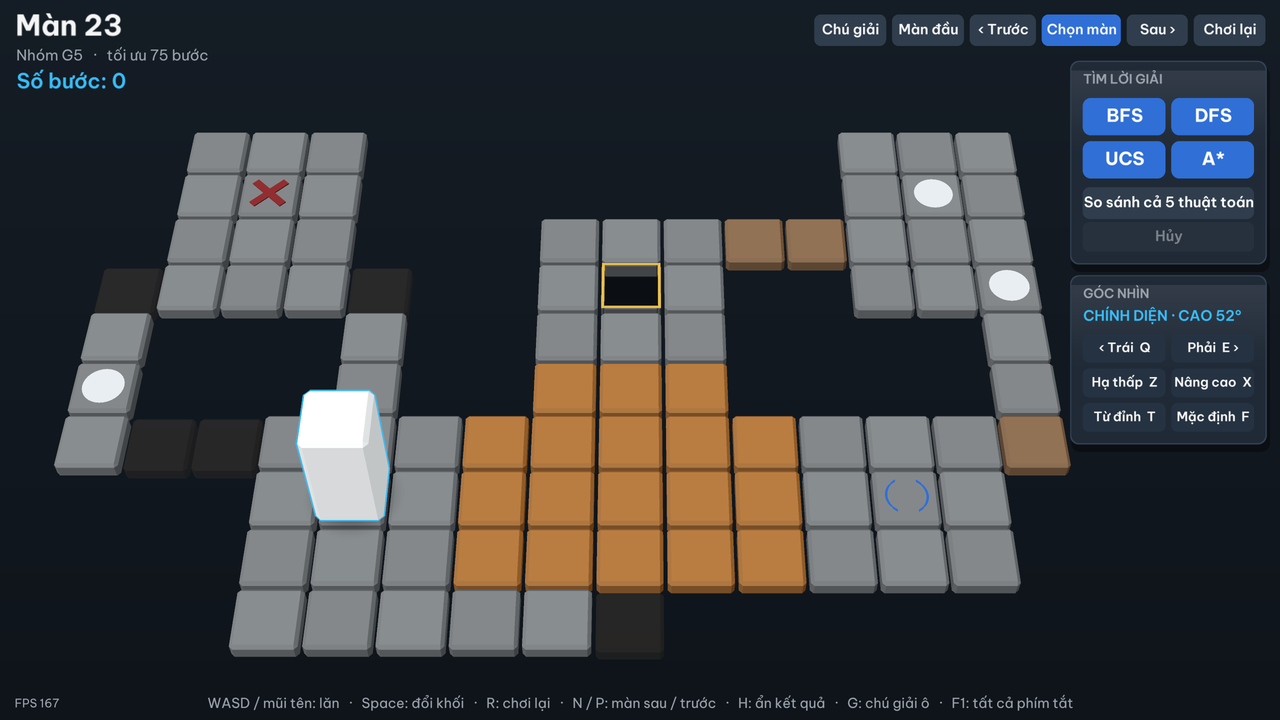
\includegraphics[width=0.86\linewidth,height=\textheight,keepaspectratio,alt={Hình 4.1}]{hinh/h4-1-man23-du-loai-o.png}
\caption{Hình 4.1. Màn 23 lúc bắt đầu: đủ 9 loại ô trên cùng một bàn, phân biệt được bằng màu và hình.}
\end{figure}

Bảng chú giải (Hình 4.11) là một lớp phủ giữa màn hình như bảng phím tắt: mỗi mục có một ô mẫu, tên và cách ô hoạt động theo luật. Ô mẫu vẽ bằng đúng màu và ký hiệu của bàn (lấy từ \texttt{board\_\allowbreak{}view.\allowbreak{}COLORS}), nên đổi màu ô trên bàn thì chú giải đổi theo. Khi bảng đang mở, phím lăn và Enter bị bỏ qua; G hoặc Esc đóng bảng.

\begin{figure}
\centering
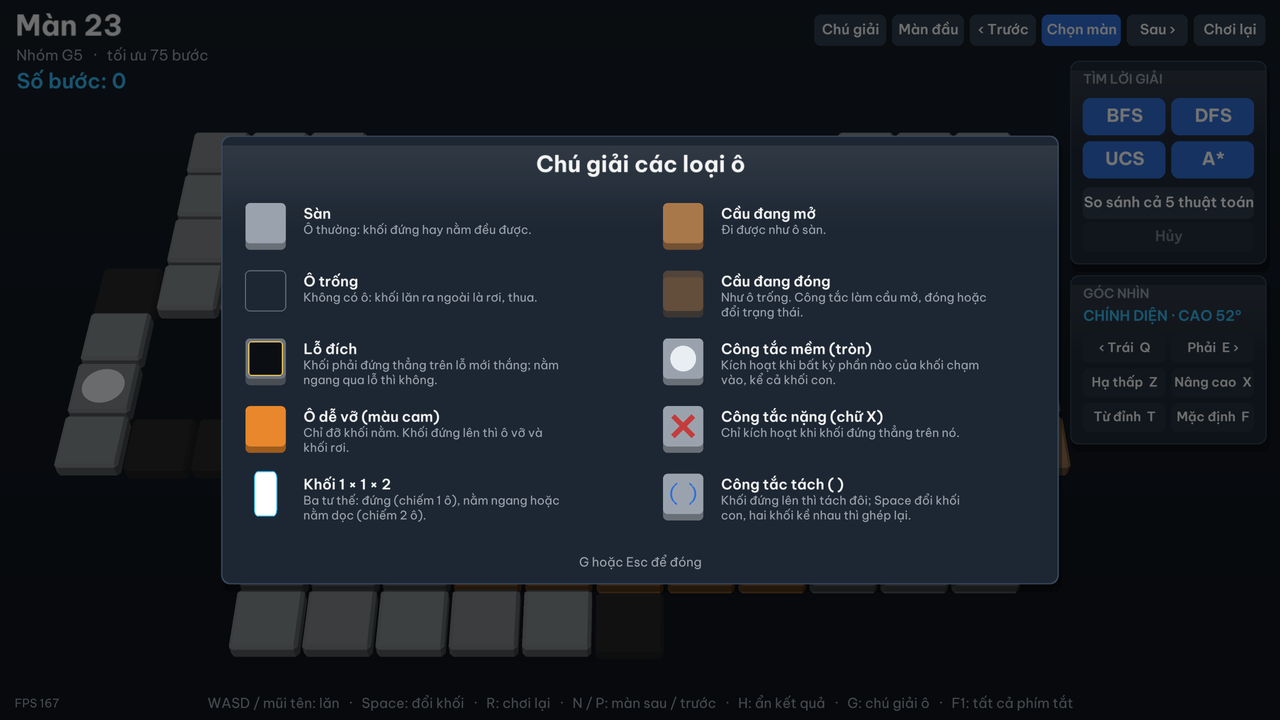
\includegraphics[width=0.86\linewidth,height=\textheight,keepaspectratio,alt={Hình 4.11}]{hinh/h4-11-chu-giai.png}
\caption{Hình 4.11. Bảng chú giải các loại ô (phím G) trên màn 23: cột trái là ô và khối, cột phải là cầu và ba loại công tắc.}
\end{figure}

\begin{longtable}[]{@{}
  >{\raggedright\arraybackslash}p{(\linewidth - 4\tabcolsep) * \real{0.2500}}
  >{\raggedright\arraybackslash}p{(\linewidth - 4\tabcolsep) * \real{0.2612}}
  >{\raggedright\arraybackslash}p{(\linewidth - 4\tabcolsep) * \real{0.4888}}@{}}
\caption{\textbf{Bảng 4.1.} Cách vẽ từng loại ô.}\tabularnewline
\toprule\noalign{}
\begin{minipage}[b]{\linewidth}\raggedright
\textbf{Ô}
\end{minipage} & \begin{minipage}[b]{\linewidth}\raggedright
\textbf{Ký hiệu trong file màn}
\end{minipage} & \begin{minipage}[b]{\linewidth}\raggedright
\textbf{Cách vẽ}
\end{minipage} \\
\midrule\noalign{}
\endfirsthead
\toprule\noalign{}
\begin{minipage}[b]{\linewidth}\raggedright
\textbf{Ô}
\end{minipage} & \begin{minipage}[b]{\linewidth}\raggedright
\textbf{Ký hiệu trong file màn}
\end{minipage} & \begin{minipage}[b]{\linewidth}\raggedright
\textbf{Cách vẽ}
\end{minipage} \\
\midrule\noalign{}
\endhead
\bottomrule\noalign{}
\endlastfoot
Sàn, ô xuất phát & \texttt{\#}, \texttt{S} & Khối hộp xám \\
Ô trống & \texttt{.\allowbreak{}} & Không vẽ gì \\
Đích & \texttt{G} & Lỗ vuông tối, viền vàng nhấp nháy nhẹ để dễ tìm \\
Ô dễ vỡ & \texttt{F} & Khối hộp cam \\
Công tắc mềm & \texttt{o} & Sàn có đĩa tròn trắng \\
Công tắc nặng & \texttt{x} & Sàn có hình X đỏ \\
Công tắc tách & \texttt{@} & Sàn có hình ``( )'' xanh \\
Cầu mở & \texttt{B} (hoặc \texttt{b} sau khi mở) & Khối hộp màu gỗ \\
Cầu đóng & \texttt{b} (hoặc \texttt{B} sau khi đóng) & Khối hộp sẫm, gần trong suốt, nhìn rõ chỗ có cầu \\
\end{longtable}

Khối 1×1×2 màu trắng có viền xanh sáng để nổi trên sàn xám, và có ba tư thế (Hình 4.2). Kích thước khối nhỏ hơn ô một chút để luôn thấy viền giữa khối và sàn. Ô và khối là hộp vát cạnh, mặt bên tối hơn mặt trên, nên bàn có độ dày mà không cần đèn mạnh. Cảnh không dùng bóng đổ thật: bóng của khối phủ lên ô làm màu ô khó phân biệt, nhất là ô dễ vỡ và cầu đóng. Thay vào đó, dưới mỗi khối có một vệt bóng mềm, nhạt dần khi khối nhấc lên, đủ để thấy khối đang chạm sàn. Cạnh ô và khối được khử răng cưa (multisample 4×).

\begin{figure}
\centering
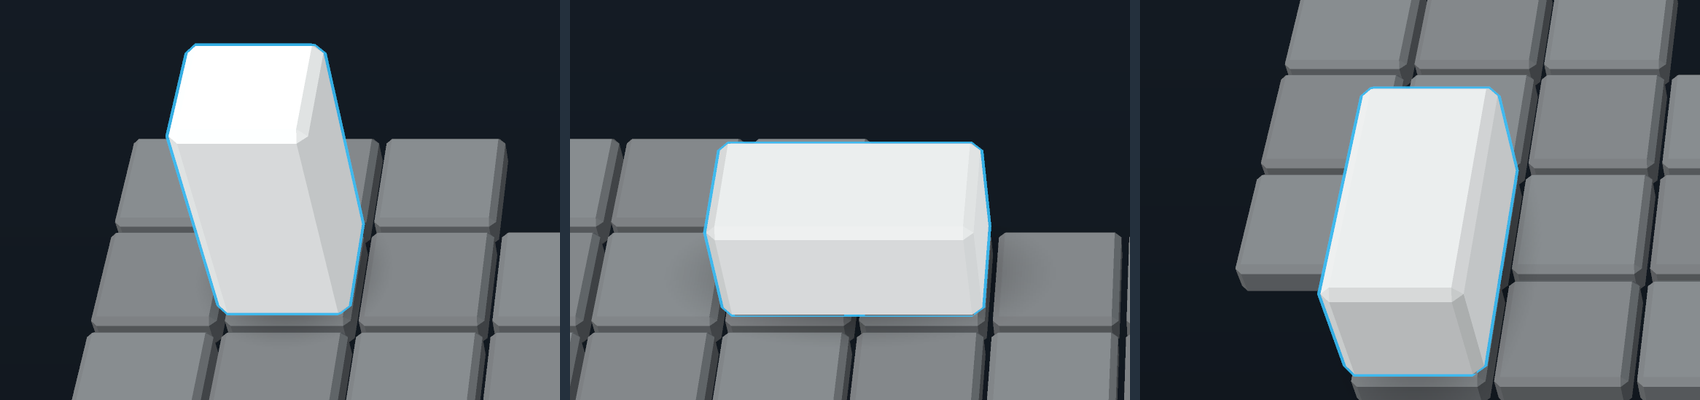
\includegraphics[width=0.86\linewidth,height=\textheight,keepaspectratio,alt={Hình 4.2}]{hinh/h4-2-ba-tu-the.png}
\caption{Hình 4.2. Ba tư thế của khối ở màn 1: đứng chiếm một ô, nằm ngang (sau phím →) và nằm dọc (sau phím ↓) chiếm hai ô.}
\end{figure}

Khi công tắc tác động, cầu bị điều khiển đổi màu dần giữa màu gỗ và màu sẫm, kèm một dòng thông báo cho biết loại công tắc và hiệu ứng (Hình 4.3). Thông báo lấy từ sự kiện \texttt{switch} của engine, không do giao diện tự suy ra.

\begin{figure}
\centering
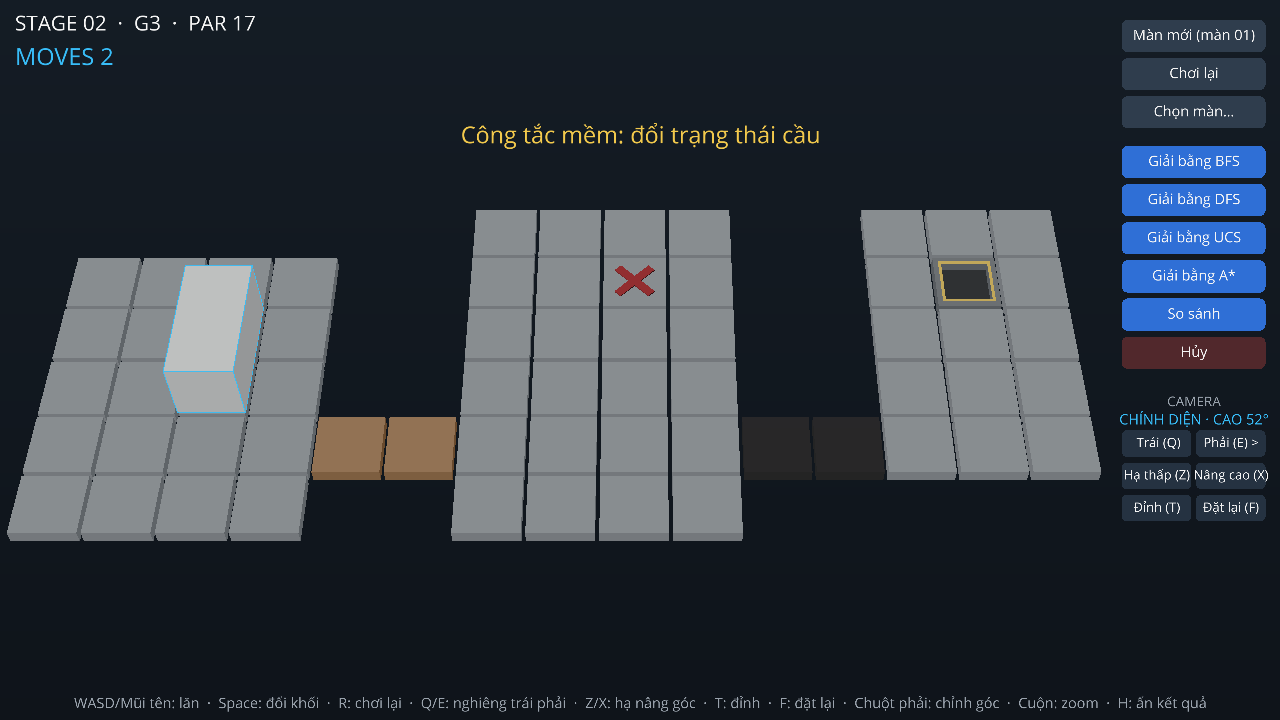
\includegraphics[width=0.86\linewidth,height=\textheight,keepaspectratio,alt={Hình 4.3}]{hinh/h4-3-cong-tac-va-cau.png}
\caption{Hình 4.3. Màn 2, bước 2: khối nằm vừa chạm công tắc mềm nên cặp cầu bên trái mở; cặp cầu bên phải vẫn đóng cho tới khi khối đứng lên công tắc nặng (dấu X đỏ).}
\end{figure}

Khi khối đứng lên công tắc tách, hai khối con bay theo đường vòng cung từ chỗ khối cũ tới hai ô định sẵn (Hình 4.4). Khối con đang điều khiển màu trắng, viền xanh rõ; khối còn lại màu xám, viền mờ; phím Space đổi khối. Engine luôn sắp hai khối con theo thứ tự ô, nên sau mỗi bước, giao diện tìm lại khối vừa đi theo ô mới của nó để giữ đúng khối người chơi đang điều khiển. Hai khối con kề nhau thì tự ghép lại, có thông báo.

\begin{figure}
\centering
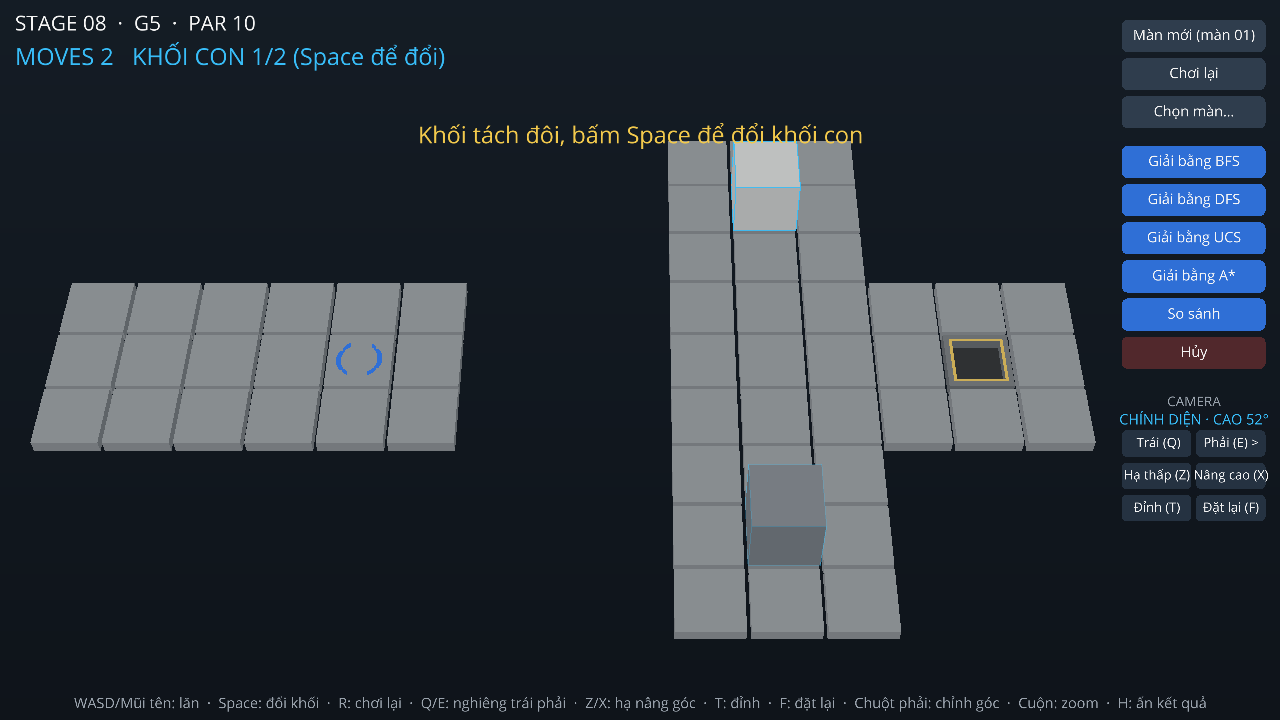
\includegraphics[width=0.86\linewidth,height=\textheight,keepaspectratio,alt={Hình 4.4}]{hinh/h4-4-tach-khoi.png}
\caption{Hình 4.4. Màn 8 sau khi tách: khối con sáng màu là khối đang điều khiển (ghi ``KHỐI CON 1/2'' cạnh số bước).}
\end{figure}

Khối rơi khi chạm ô trống, ra ngoài bàn, vào cầu đóng, hoặc đứng thẳng trên ô dễ vỡ. Giao diện hiện lý do rơi; với ô dễ vỡ, ô cam rơi cùng khối (Hình 4.5) và được dựng lại khi bấm R. Khối nằm mà chỉ một đầu hụt thì đổ nghiêng qua mép ô còn đỡ rồi mới rơi, không xuyên qua sàn; khi đã tách, chỉ khối con bị hụt rơi. Khối mờ dần khi rơi xuống dưới bàn. Việc chọn kiểu đổ chỉ dựa vào hình (ô nào còn tấm đỡ); quyết định có rơi hay không vẫn do \texttt{rules.\allowbreak{}step()}.

\begin{figure}
\centering
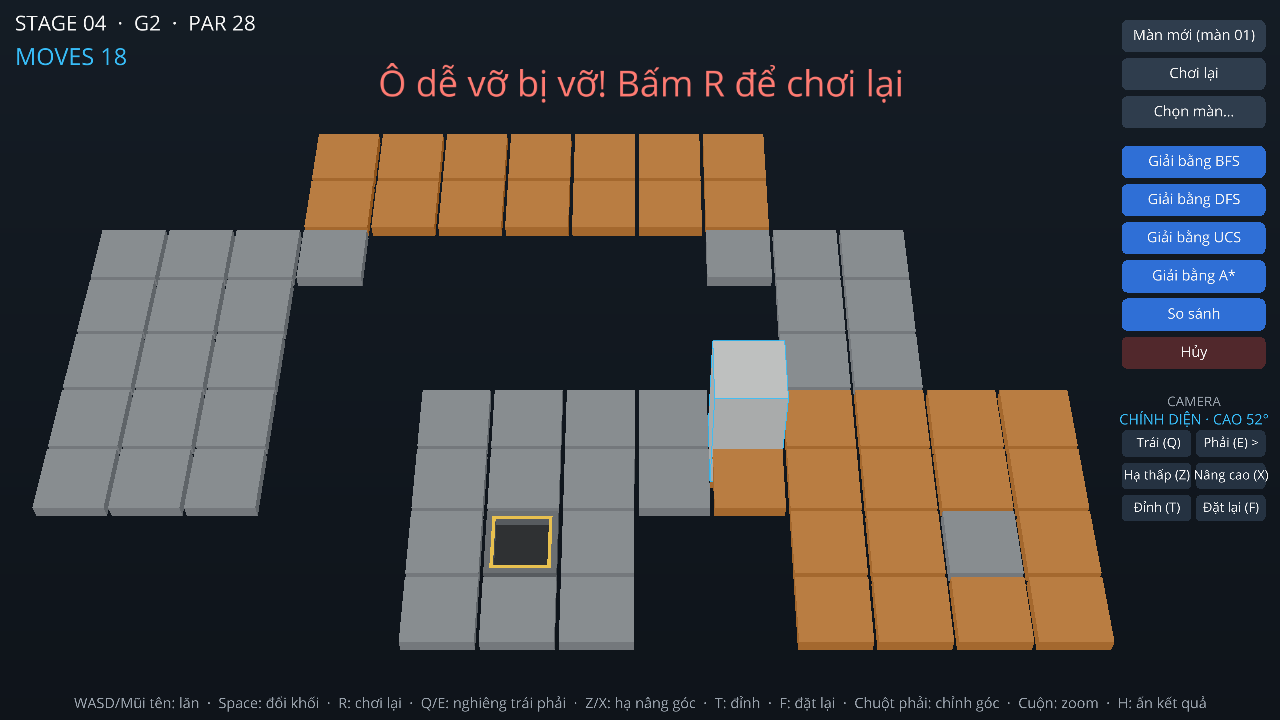
\includegraphics[width=0.86\linewidth,height=\textheight,keepaspectratio,alt={Hình 4.5}]{hinh/h4-5-o-de-vo.png}
\caption{Hình 4.5. Màn 4, bước 18: khối đứng thẳng lên ô dễ vỡ, ô cam vỡ và đang rơi cùng khối (giữa phía dưới); hộp kết thúc (được kéo lên mép trên) nêu đúng lý do thua.}
\end{figure}

\subsection{4.5. Chơi tay}

\textbf{Trang chủ.} Chạy \texttt{python main.\allowbreak{}py} không kèm số màn thì trang chủ hiện ra: bàn 3D của màn 1 xoay chậm phía sau, bên trái là tên game và bốn nút Chơi ngay, Chọn màn, Cách chơi, Thoát (chọn bằng chuột, hoặc bằng phím mũi tên rồi Enter). Nút Cách chơi mở bảng hướng dẫn bốn trang, mỗi trang có một bàn mô phỏng tự chạy: mục tiêu của màn, cách lăn khối, khi nào thì thua, các ô đặc biệt và cách nhờ thuật toán giải. Trong lúc chơi, nút Trang chủ hoặc phím M đưa về trang chủ. Các phím khi chơi:

{\def\LTcaptype{none} % do not increment counter
\begin{longtable}[]{@{}
  >{\raggedright\arraybackslash}p{(\linewidth - 2\tabcolsep) * \real{0.3777}}
  >{\raggedright\arraybackslash}p{(\linewidth - 2\tabcolsep) * \real{0.6223}}@{}}
\toprule\noalign{}
\begin{minipage}[b]{\linewidth}\raggedright
\textbf{Phím}
\end{minipage} & \begin{minipage}[b]{\linewidth}\raggedright
\textbf{Tác dụng}
\end{minipage} \\
\midrule\noalign{}
\endhead
\bottomrule\noalign{}
\endlastfoot
← ↑ → ↓ hoặc W A S D & Lăn khối \\
Space & Đổi khối con (khi đã tách) \\
R & Chơi lại màn \\
M & Về trang chủ \\
N / P & Màn sau / màn trước \\
Q / E, Z / X, T, F, chuột phải, con lăn & Đổi góc nhìn (mục 4.7) \\
H & Ẩn hoặc hiện khung kết quả (mục 4.7) \\
Ctrl+K & Mở hoặc đóng lưới chọn màn \\
Enter & Nút chính của hộp kết thúc màn \\
G & Bảng chú giải các loại ô (Hình 4.11) \\
F1 & Bảng tất cả phím tắt \\
Esc & Đóng hộp kết thúc màn, lưới chọn màn, bảng phím tắt hoặc bảng chú giải \\
\end{longtable}
}

Một lượt đi diễn ra theo thứ tự: phím được đổi thành hành động và gửi vào \texttt{rules.\allowbreak{}step()}; khối lật 90° quanh cạnh đáy theo hướng đi, tới vị trí ngay sau khi lăn (khối được gắn tạm vào một trục đặt ở cạnh đó rồi xoay trục; lật xong thì đặt lại đúng vị trí và góc theo trạng thái, nên sai số không dồn qua các bước); sau đó giao diện cập nhật cầu, hiện thông báo sự kiện, rồi vẽ trạng thái cuối (tách, ghép, rơi hoặc thắng). Trong lúc hoạt ảnh chạy, phím mới bị bỏ qua, để trạng thái giao diện đang giữ không đi trước hình đang vẽ. Mỗi lần chơi lại hoặc đổi màn, giao diện tăng một số đếm lượt; lệnh hẹn giờ nào của lượt cũ còn sót lại thấy số đếm đã đổi thì bỏ qua, nên bấm R giữa lúc khối đang lăn không làm trạng thái cũ ghi đè lên màn vừa chơi lại.

Mọi đối tượng của một màn gắn vào một gốc chung; đổi màn thì hủy gốc này, nên bàn cũ không còn sót lại. Đây là một trong các lỗi hay gặp với Ursina mà nhóm khóa trước ghi lại {[}8{]}. Ursina 7 còn một lỗi tương tự với hoạt ảnh hẹn giờ (\texttt{animate(.\allowbreak{}.\allowbreak{}.\allowbreak{}, delay=.\allowbreak{}.\allowbreak{}.\allowbreak{})}): lần hẹn không được ghi lại nên không hủy được, và nếu đổi màn trước lúc tới giờ thì nó chạy trên đối tượng đã bị hủy, làm cửa sổ dừng. Giao diện dùng hàm hẹn giờ riêng (\texttt{gui/\allowbreak{}anim.\allowbreak{}py}), hủy được và tự bỏ qua khi đối tượng đã bị hủy.

Khi vào màn, các ô trồi lên lần lượt theo đường chéo rồi khối rơi xuống chỗ xuất phát; công tắc lún xuống khi tác động; cầu vừa mở trồi lên, cầu vừa đóng mờ đi và lún xuống; khi thắng, viền ô đích lóe sáng và một vòng sáng lan ra. Trong lúc khối rơi xuống chỗ xuất phát, phím lăn bị bỏ qua như mọi hoạt ảnh khác.

\subsection{4.6. Giải tự động và So sánh}

Các nút được nhóm theo việc. Thanh trên cùng bên phải là điều hướng màn: Trang chủ, Chú giải (Hình 4.11), Màn đầu, ‹ Trước, Chọn màn (Hình 4.9), Sau ›, Chơi lại. Hai nút điều khiển cơ bản mà đề yêu cầu là \textbf{Màn đầu} (New Game: bắt đầu lại từ màn 1) và \textbf{Chơi lại} (Restart: đặt khối, cầu và ô dễ vỡ của màn đang chơi về trạng thái đầu, như phím R). Cột bên phải có hai thẻ: thẻ ``Tìm lời giải'' gồm lưới 2 × 2 nút giải (Solve) BFS, DFS, UCS, A*, nút So sánh cả 5 thuật toán và nút Hủy; thẻ ``Góc nhìn'' gồm nhãn góc hiện tại và 6 nút camera. Nút không dùng được lúc đó chuyển sang màu xám (khi chưa chạy thì Hủy xám, khi đang chạy thì các nút giải xám). Trong lúc giải, một khung sáng bao quanh nút của thuật toán đang chạy (khi So sánh, khung trượt dần qua từng nút), và chấm trước dòng đầu của khung kết quả nhấp nháy; xong thì chấm đổi màu theo kết quả.

\textbf{Hộp kết thúc màn.} Khi thắng hoặc rơi, sau khi hoạt ảnh gần xong, một hộp hiện giữa vùng bàn (không che khung kết quả và cột nút). Khi thắng, hộp ghi số bước so với số bước tối ưu, và tên thuật toán nếu khối vừa tự lăn theo lời giải; nút chính là Màn tiếp. Khi rơi, hộp ghi lý do (ô dễ vỡ, cầu đóng, hụt khỏi bàn) theo sự kiện của engine; nút chính là Chơi lại. Enter bấm nút chính, Esc đóng hộp; chơi lại hay đổi màn thì hộp tự đóng. Hộp kéo thả được: giữ chuột trái ở chỗ bất kỳ trên hộp (trừ các nút, có dấu tay nắm ở mép trên) rồi kéo; hộp không ra khỏi màn hình, và các lần sau hiện lại ở chỗ đã kéo tới. Bấm Giải hoặc So sánh thì hộp của lượt trước đóng lại.

\textbf{Chạy thuật toán không làm đơ giao diện.} Ursina vẽ mọi thứ trong một vòng lặp duy nhất, nên nếu chạy thuật toán ngay trong vòng lặp đó thì cửa sổ đứng yên suốt lúc tìm. Khi bấm một nút Giải, giao diện gọi \texttt{runner.\allowbreak{}start\_\allowbreak{}solver()}; hàm này mở một tiến trình con chạy thuật toán rồi trả về ngay. Mỗi khung hình, giao diện gọi \texttt{poll()} để hỏi kết quả mà không phải chờ; không dùng callback từ tiến trình khác, vì Ursina không an toàn khi đối tượng bị sửa ngoài luồng chính. Dùng tiến trình chứ không dùng luồng vì Python không dừng ngang được một luồng: quá 60 giây hoặc khi bấm Hủy, tiến trình con bị dừng hẳn. Trong lúc chờ, khung kết quả hiện tên thuật toán và số giây đã chạy, các nút Giải mờ đi và nút Hủy sáng lên (Hình 4.7). Khi đo trong lúc thuật toán chạy, khung hình chậm nhất khoảng 55 ms, tức cửa sổ vẫn phản hồi.

Mỗi lần giải có bốn kết quả, mỗi loại một thông báo và màu riêng: \textbf{giải được}, \textbf{không có lời giải}, \textbf{hết giờ}, \textbf{lỗi hoặc đã hủy}. Khi giải được, màn được đặt lại về trạng thái đầu và khối tự lăn theo lời giải, mỗi bước cũng qua \texttt{rules.\allowbreak{}step()} như khi chơi tay. Khung kết quả ở cột bên trái hiện số bước, tổng chi phí, số nút được mở rộng và được sinh, kích thước biên lớn nhất, số trạng thái đã thăm, thời gian tìm kiếm (không tính thời gian hoạt ảnh) và bộ nhớ đỉnh (Hình 4.6).

\begin{figure}
\centering
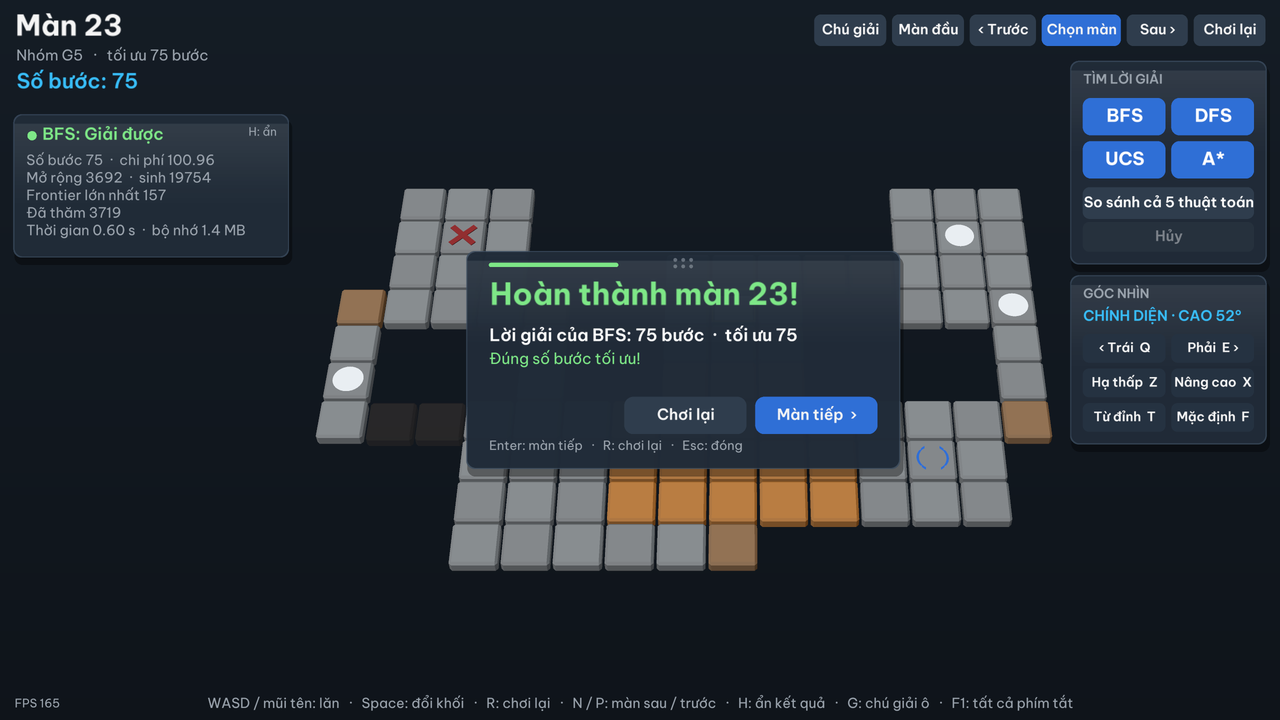
\includegraphics[width=0.86\linewidth,height=\textheight,keepaspectratio,alt={Hình 4.6}]{hinh/h4-6-giai-bfs-thang.png}
\caption{Hình 4.6. Màn 23 sau khi bấm Giải bằng BFS: khối đã tự lăn tới đích sau 75 bước, đúng số bước tối ưu; khung kết quả hiện các chỉ số của lần tìm, bàn thu nhỏ vào phần màn hình còn trống nên không bị che.}
\end{figure}

\textbf{So sánh} chạy lần lượt năm thuật toán trên màn đang mở: BFS, DFS, UCS, A* với \(h_P\) và A* với \(h_M\), mỗi thuật toán một tiến trình. Chạy lần lượt chứ không song song để thời gian và bộ nhớ của các thuật toán không ảnh hưởng nhau. Bảng được điền dần khi từng thuật toán xong (Hình 4.7, 4.8); dòng đang chạy ghi số giây đã chạy; thuật toán nào lỗi thì ô ghi ``Lỗi'' và nội dung lỗi ghi dưới bảng. Cột ``Giây'' và ``MB'' ghi số không kèm đơn vị cho bảng gọn.

\begin{figure}
\centering
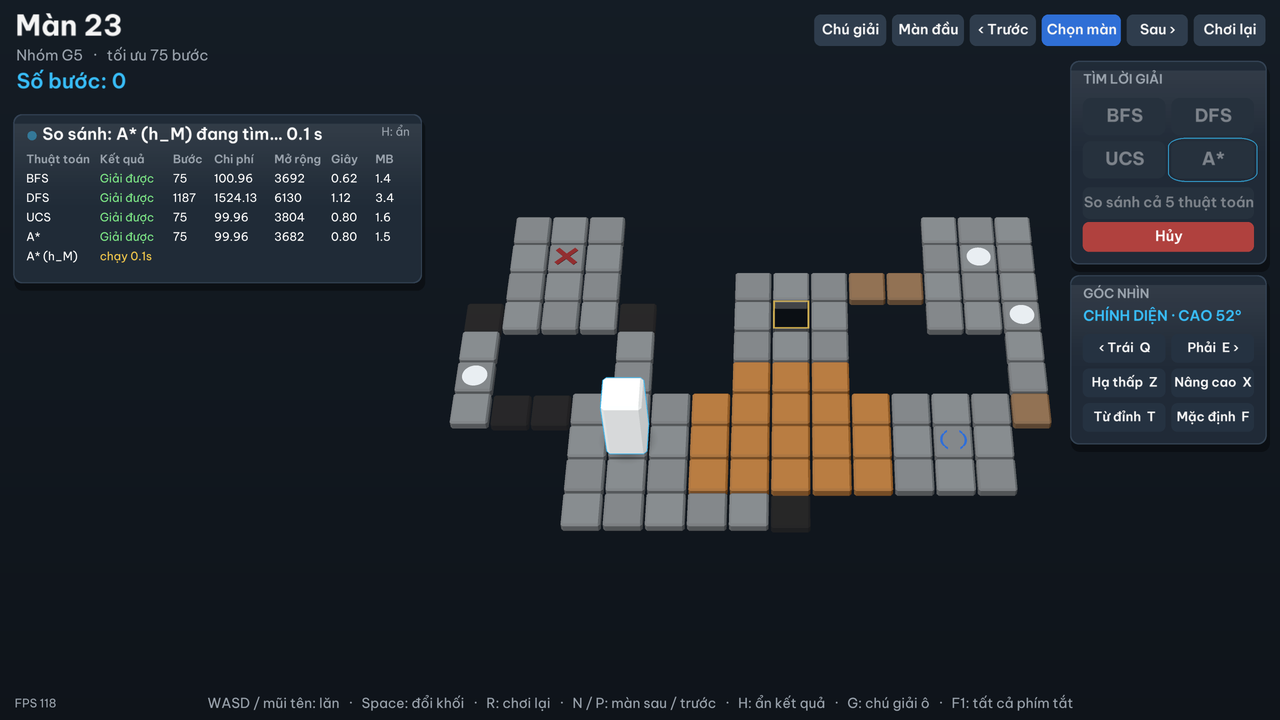
\includegraphics[width=0.86\linewidth,height=\textheight,keepaspectratio,alt={Hình 4.7}]{hinh/h4-7-so-sanh-dang-chay.png}
\caption{Hình 4.7. So sánh đang chạy trên màn 23: bốn thuật toán đã xong, A}
\end{figure}

\begin{figure}
\centering
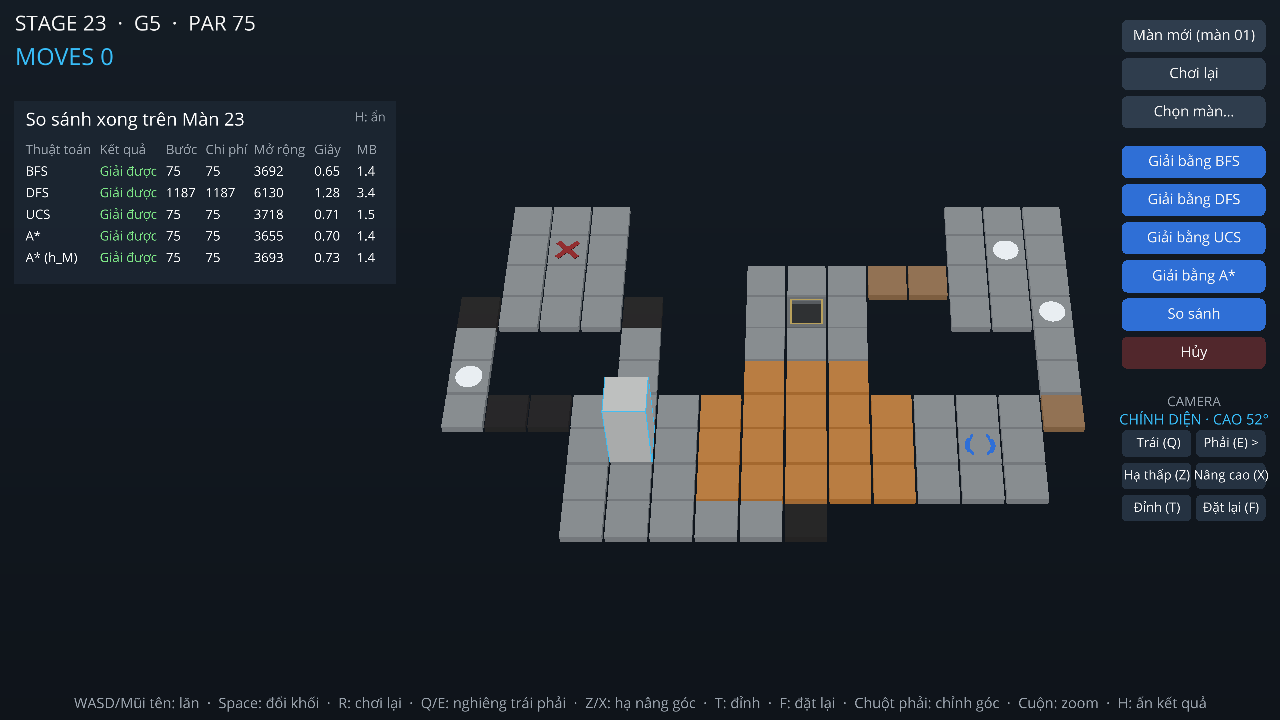
\includegraphics[width=0.86\linewidth,height=\textheight,keepaspectratio,alt={Hình 4.8}]{hinh/h4-8-so-sanh-xong.png}
\caption{Hình 4.8. Kết quả So sánh trên màn 23: BFS, UCS và A}
\end{figure}

Nút Giải và So sánh dựng bài toán với hàm chi phí ở mục 3.3, nên cột Chi phí của cả năm thuật toán tính theo cùng một hàm (mục 3.3.2): BFS cho số bước ít nhất, UCS và A* cho tổng chi phí nhỏ nhất. Ở màn 23, BFS đi 75 bước tốn 101,58, còn UCS và A* đi 75 bước khác tốn 100,58.

Thời gian và bộ nhớ trên giao diện chỉ để tham khảo, vì tiến trình con luôn bật \texttt{tracemalloc} để đo bộ nhớ, và việc này làm chậm thuật toán. Số liệu ở chương 5 lấy từ script thực nghiệm.

\begin{figure}
\centering
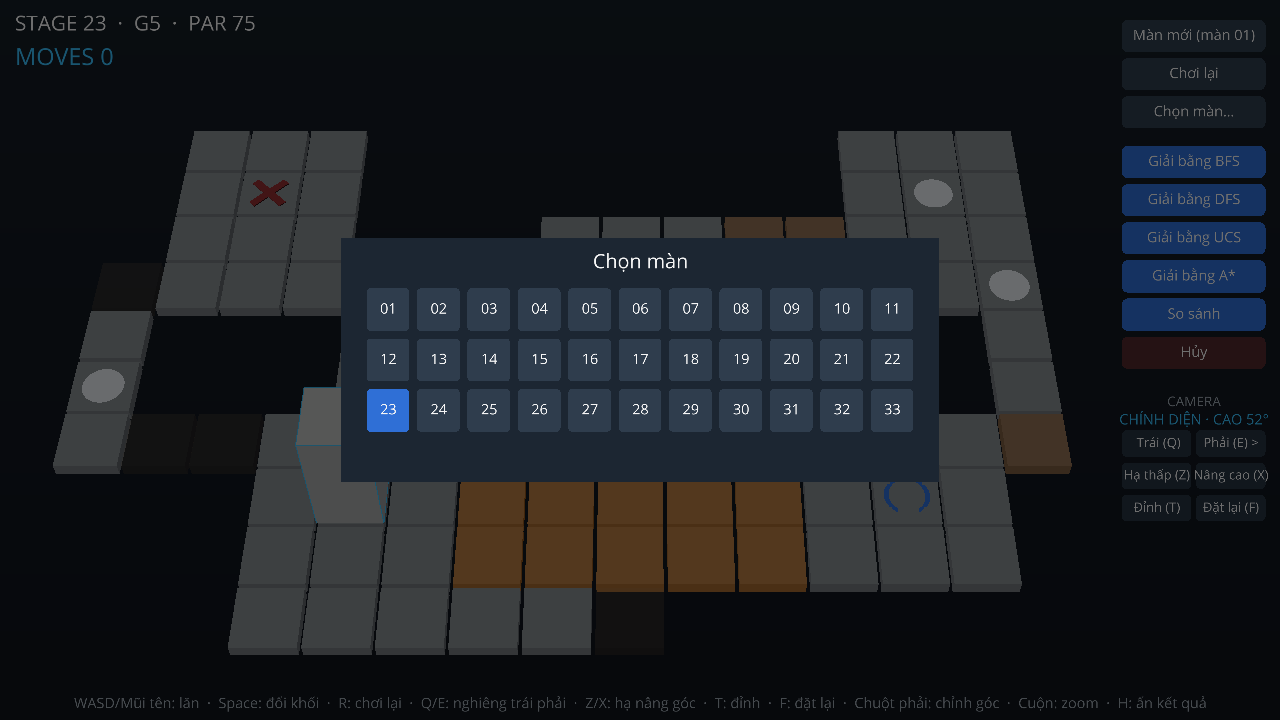
\includegraphics[width=0.86\linewidth,height=\textheight,keepaspectratio,alt={Hình 4.9}]{hinh/h4-9-chon-man.png}
\caption{Hình 4.9. Lưới chọn màn: màn đang mở tô màu xanh; bấm một mã màn để chuyển thẳng tới màn đó, thuật toán đang chạy (nếu có) bị hủy. Bấm ra ngoài lưới, Esc hoặc Ctrl+K để đóng. Màn đã thắng trong lần chạy này có chấm xanh ở góc nút.}
\end{figure}

\subsection{4.7. Camera và bố cục màn hình}

Camera xoay quanh tâm bàn và \textbf{luôn nhìn từ trên xuống, từ phía người chơi}. Nếu cho xoay tự do 360°, người chơi dễ lẫn hướng: khi camera quay quá 45°, phím ↑ không còn đẩy khối ``ra xa màn hình'' nữa. Vì vậy góc nhìn chỉ đổi trong vùng giới hạn (Hình 4.10):

\begin{itemize}
\tightlist
\item
  \textbf{Nghiêng trái, phải} (Q / E): năm nấc 40° trái, 20° trái, chính diện, 20° phải, 40° phải. Góc lệch luôn dưới 45° nên bốn phím mũi tên giữ nguyên nghĩa trên màn hình, giao diện không phải đổi lại hướng phím.
\item
  \textbf{Hạ thấp, nâng cao} (Z / X): góc giữa mặt bàn và hướng nhìn có bốn nấc 52°, 45°, 38°, 30°. Góc thấp thấy rõ khối đứng và độ cao của khối, góc cao thấy rõ toàn bàn; người chơi chọn nấc thấy dễ nhìn.
\item
  \textbf{Nhìn từ đỉnh} (T): nhìn thẳng xuống, bàn thẳng hàng với màn hình; bấm T lần nữa thì trở về góc trước đó. Góc đỉnh đặt 88,5° chứ không đúng 90° để phép tính hướng nhìn không bị suy biến.
\item
  \textbf{Kéo chuột phải} chỉnh góc liên tục nhưng vẫn trong vùng trên; \textbf{con lăn} thu phóng; \textbf{F} về góc mặc định (chính diện, 52°). Góc đã chọn được giữ khi đổi màn.
\end{itemize}

Camera chuyển góc mượt bằng nội suy mỗi khung hình. Khi nghiêng ngang, camera lùi xa thêm một chút vì bàn chiếm chỗ theo đường chéo; hướng ``lên'' của camera luôn ghim theo trục y nên hình không bị xoay nghiêng dần sau nhiều lần đổi góc. Tên góc đang dùng (ví dụ ``CHÍNH DIỆN · CAO 52°'') hiện trên nhóm nút camera.

\begin{figure}
\centering
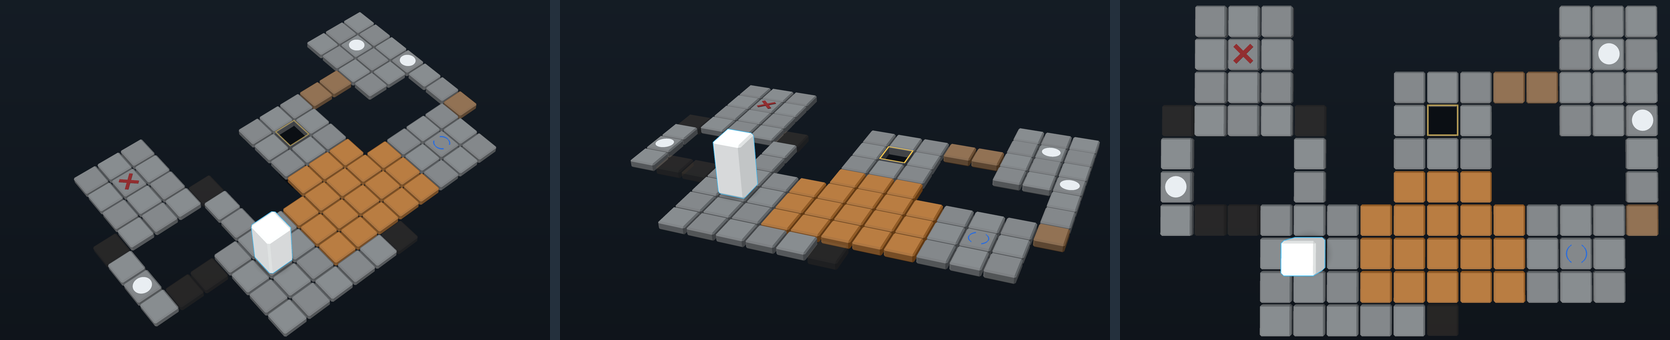
\includegraphics[width=0.86\linewidth,height=\textheight,keepaspectratio,alt={Hình 4.10}]{hinh/h4-10-goc-camera.png}
\caption{Hình 4.10. Màn 23 ở ba góc nhìn: nghiêng trái 40° (cao 52°), nghiêng phải 20° hạ thấp còn 30°, và nhìn từ đỉnh. Ở cả ba góc, phím ↑ vẫn đẩy khối về phía trên màn hình.}
\end{figure}

\textbf{Bố cục khi khung kết quả hiện.} Khung kết quả nằm ở cột bên trái, gọn theo nội dung: rộng vừa các chỉ số khi giải bằng một thuật toán, rộng vừa bảng khi So sánh (vị trí cột tính theo bề rộng chữ thật). Bàn chỉ bị dời hoặc thu khi thật sự bị khung che: giao diện chiếu các góc ô qua camera để biết bàn chiếm đoạn nào trên màn hình. Nếu bàn đã nằm ngoài khung thì giữ nguyên; nếu chạm khung thì ưu tiên dời ngang (bằng độ lệch ống kính, góc nhìn không đổi), chỉ khi dời không đủ mới lùi camera, và chỉ lùi vừa đủ để bàn nằm gọn giữa khung và cột nút (Hình 4.6, 4.8). Đổi góc camera trong lúc khung đang hiện thì bàn được đo và căn lại. Phím H ẩn khung; kết quả lần giải mới luôn hiện lại khung.

Khung kết quả, hộp kết thúc và các thẻ nút có nền hơi trong (vẫn thấy lờ mờ bàn phía sau), viền mảnh, một dải sáng rất nhẹ ở mép trên mờ dần xuống và bóng mềm phía dưới, để tách khỏi nền mà không che hẳn bàn.

\subsection{4.8. Kiểm thử giao diện}

Ngoài unit test của engine và thuật toán (không cần Ursina), giao diện được thử bằng các script mở cửa sổ thật và tự bấm phím, bấm nút thay người chơi. Các dòng có ghi 29/10 được chạy lại trên giao diện hiện tại; các dòng còn lại chạy ngày 23/10 và phần code liên quan chưa đổi từ đó.

{\def\LTcaptype{none} % do not increment counter
\begin{longtable}[]{@{}
  >{\raggedright\arraybackslash}p{(\linewidth - 2\tabcolsep) * \real{0.5660}}
  >{\raggedright\arraybackslash}p{(\linewidth - 2\tabcolsep) * \real{0.4340}}@{}}
\toprule\noalign{}
\begin{minipage}[b]{\linewidth}\raggedright
\textbf{Kiểm tra}
\end{minipage} & \begin{minipage}[b]{\linewidth}\raggedright
\textbf{Kết quả}
\end{minipage} \\
\midrule\noalign{}
\endhead
\bottomrule\noalign{}
\endlastfoot
Chơi tay theo lời giải BFS ở màn 2, 4, 8 (cầu, ô dễ vỡ, tách và ghép) & Thắng đúng 17, 28, 10 bước \\
Đứng lên ô dễ vỡ ở màn 4, rồi bấm R & Rơi, đúng thông báo; ô được dựng lại \\
Bấm R giữa lúc khối đang lăn & Không bị lượt cũ ghi đè \\
Giải bằng BFS rồi tự lăn, trên cả 33 màn (29/10) & 33/33 màn thắng đúng số bước tối ưu \\
Giải bằng DFS rồi tự lăn ở màn 1, 8, 16, 23, 29 & Thắng ở cả 5 màn (màn 23: 1187 bước) \\
So sánh trên cả 33 màn & 33/33 màn đủ năm dòng kết quả \\
So sánh trên màn 23 (29/10) & Đủ năm dòng; BFS, UCS, A* (\(h_P\)), A* (\(h_M\)) 75 bước, DFS 1187 bước \\
Bấm Hủy khi đang giải và khi đang So sánh; đổi màn khi đang giải & Dừng đúng; các nút trở lại trạng thái ban đầu \\
Đổi qua mọi nấc Q/E, Z/X, T rồi F (29/10) & Camera dừng đúng nấc, hình không bị xoay nghiêng; F về chính diện 52° \\
Khung kết quả hiện, rồi bấm H (29/10) & Bàn thu vào phần còn trống, không bị che; ẩn khung thì bàn về cỡ đầy đủ \\
Cài trong môi trường ảo mới theo README & Cài đúng phiên bản, test qua, cửa sổ mở được \\
Giải bằng BFS rồi tự lăn trên cả 33 màn, với hoạt ảnh lật khối mới (30/10) & 33/33 màn thắng đúng số bước tối ưu \\
Bấm phím ngẫu nhiên mỗi khung hình (lăn, R, N, P, Space, camera, Ctrl+K) xen với Giải, So sánh, Hủy; 17 lần × 35 giây (30/10) & Không lỗi, không treo (trước khi sửa hoạt ảnh hẹn giờ: 4/12 lần dừng vì lỗi \texttt{!is\_\allowbreak{}empty()}) \\
Kéo hộp kết thúc bằng chuột (giả lập), kéo ra ngoài màn hình, bấm vào nút trong hộp (30/10) & Hộp đi theo chuột, dừng ở mép màn hình; bấm nút không kéo hộp; lần thắng sau hộp hiện ở chỗ đã kéo \\
Khung kết quả hiện ở màn 23 (một thuật toán, rồi So sánh) (30/10) & Bàn giữ nguyên cỡ khi không bị che; khi So sánh chỉ thu vừa đủ \\
Thắng ở màn 1; bấm F1, Esc; rơi ở màn 1 (30/10) & Khối thu vừa miệng lỗ và nhìn thấy trong lòng lỗ; hộp thắng ghi đúng số bước; hộp rơi ghi đúng lý do \\
Lăn ra mép ở màn 1 (một đầu hụt, rồi hụt cả hai đầu), tách và ghép ở màn 8, đứng lên ô dễ vỡ, rồi bấm R (30/10) & Khối đổ nghiêng qua mép, không xuyên sàn; chỉ khối con hụt rơi; ô dễ vỡ được dựng lại \\
Rà soát giao diện: Hủy khi khối tự lăn, bấm R khi cầu đang đổi, Giải/So sánh ngay sau khi rơi, chữ trong khung kết quả, Enter khi mở F1, thu phóng khi khung hiện (30/10) & 6 lỗi tái hiện được trước khi sửa, không còn sau khi sửa \\
Bảng chú giải: G, nút ``Chú giải'', Esc, F1 khi bảng đang mở; Enter và phím lăn khi bảng đang mở (31/10) & Mở, đóng đúng; F1 thay bảng chú giải; Enter và phím lăn bị bỏ qua \\
\end{longtable}
}

\subsection{4.9. Hạn chế}

\begin{itemize}
\tightlist
\item
  Chấm đánh dấu màn đã thắng chỉ giữ trong một lần chạy chương trình, chưa lưu ra file.
\item
  Chưa chỉnh được tốc độ khối tự lăn và chưa tạm dừng được giữa chừng (chỉ dừng hẳn bằng Hủy hoặc R).
\item
  Menu chọn màn chỉ có 33 màn gốc; bộ màn tự sinh S1--S3 (chương 5) chưa mở được từ giao diện.
\end{itemize}

\section{5. Thực nghiệm}

Chương này so sánh năm cấu hình thuật toán trên cùng một bộ màn, cùng một hàm chi phí và cùng một cách đo. Mục 5.1 nêu câu hỏi và cách đo, mục 5.2 mô tả bộ màn, mục 5.3 trình bày kết quả, mục 5.4 nhận xét từng thuật toán và mục 5.5 trả lời các câu hỏi.

\subsection{5.1. Thiết lập thực nghiệm}

\textbf{Câu hỏi cần trả lời.}

\begin{enumerate}
\def\labelenumi{\arabic{enumi}.}
\tightlist
\item
  Thuật toán nào mở rộng ít nút nhất, chạy nhanh nhất, tốn ít bộ nhớ nhất, và khác biệt thay đổi thế nào theo nhóm màn G1--G5?
\item
  Chất lượng lời giải: số bước và tổng chi phí so với tối ưu.
\item
  Công tắc và cầu làm không gian trạng thái lớn lên bao nhiêu (nhóm S2)?
\item
  Mỗi heuristic của A* (\(h_M\), \(h_P\)) bớt được bao nhiêu nút so với UCS?
\item
  Số nút, thời gian và bộ nhớ tăng thế nào khi bàn lớn dần (S1), và khi màn không có lời giải (S3)?
\end{enumerate}

\textbf{Thuật toán.} Năm cấu hình, dùng chung một engine luật, một hàm chi phí và một thứ tự hành động (U, D, L, R; khi đã tách U1 \ldots{} R1, U2 \ldots{} R2):

{\def\LTcaptype{none} % do not increment counter
\begin{longtable}[]{@{}
  >{\raggedright\arraybackslash}p{(\linewidth - 6\tabcolsep) * \real{0.1250}}
  >{\raggedright\arraybackslash}p{(\linewidth - 6\tabcolsep) * \real{0.4170}}
  >{\raggedright\arraybackslash}p{(\linewidth - 6\tabcolsep) * \real{0.3469}}
  >{\raggedright\arraybackslash}p{(\linewidth - 6\tabcolsep) * \real{0.1111}}@{}}
\toprule\noalign{}
\begin{minipage}[b]{\linewidth}\raggedright
\textbf{Khóa}
\end{minipage} & \begin{minipage}[b]{\linewidth}\raggedright
\textbf{Thuật toán}
\end{minipage} & \begin{minipage}[b]{\linewidth}\raggedright
\textbf{Kiểm tra đích}
\end{minipage} & \begin{minipage}[b]{\linewidth}\raggedright
\textbf{Chương}
\end{minipage} \\
\midrule\noalign{}
\endhead
\bottomrule\noalign{}
\endlastfoot
\texttt{bfs} & BFS & khi sinh nút & 3.1 \\
\texttt{dfs} & DFS dạng tìm kiếm trên đồ thị & khi sinh nút & 3.2 \\
\texttt{ucs} & UCS & khi lấy ra khỏi hàng đợi & 3.3 \\
\texttt{astar} & A* với \(h_P\) (heuristic chính) & khi lấy ra khỏi hàng đợi & 3.4 \\
\texttt{astar\_\allowbreak{}m} & A* với \(h_M\) (để so sánh) & khi lấy ra khỏi hàng đợi & 3.4 \\
\end{longtable}
}

Thời điểm kiểm tra đích làm thay đổi số nút mở rộng: BFS và DFS dừng ngay khi sinh ra đích, còn UCS và A* phải chờ tới lúc lấy đích ra để giữ tính tối ưu. Khi đọc bảng, cần nhớ điều này.

\textbf{Chỉ số.} Bốn chỉ số đề bắt buộc (thời gian tìm kiếm, bộ nhớ đỉnh, số nút mở rộng, độ dài lời giải), cộng năm chỉ số để giải thích kết quả.

\begin{longtable}[]{@{}
  >{\raggedright\arraybackslash}p{(\linewidth - 4\tabcolsep) * \real{0.2778}}
  >{\raggedright\arraybackslash}p{(\linewidth - 4\tabcolsep) * \real{0.1944}}
  >{\raggedright\arraybackslash}p{(\linewidth - 4\tabcolsep) * \real{0.5278}}@{}}
\caption{\textbf{Bảng 5.1.} Các chỉ số đo (quy ước đếm ở mục 3.1.3).}\tabularnewline
\toprule\noalign{}
\begin{minipage}[b]{\linewidth}\raggedright
\textbf{Chỉ số}
\end{minipage} & \begin{minipage}[b]{\linewidth}\raggedright
\textbf{Cột trong \texttt{summary.\allowbreak{}csv}}
\end{minipage} & \begin{minipage}[b]{\linewidth}\raggedright
\textbf{Định nghĩa}
\end{minipage} \\
\midrule\noalign{}
\endfirsthead
\toprule\noalign{}
\begin{minipage}[b]{\linewidth}\raggedright
\textbf{Chỉ số}
\end{minipage} & \begin{minipage}[b]{\linewidth}\raggedright
\textbf{Cột trong \texttt{summary.\allowbreak{}csv}}
\end{minipage} & \begin{minipage}[b]{\linewidth}\raggedright
\textbf{Định nghĩa}
\end{minipage} \\
\midrule\noalign{}
\endhead
\bottomrule\noalign{}
\endlastfoot
Số bước & \texttt{steps} & Số lần lăn trong lời giải, gồm cả bước của khối con \\
Tổng chi phí & \texttt{path\_\allowbreak{}cost} & Tổng chi phí bước dọc lời giải, theo \textbf{cùng một} hàm chi phí cho cả 5 cấu hình \\
Số nút mở rộng & \texttt{expanded} & Số trạng thái được lấy ra khỏi biên để sinh con. \textbf{Chỉ số chính khi so sánh} \\
Số nút sinh & \texttt{generated} & Số trạng thái con hợp lệ, đếm trước khi xét tập đã thăm \\
Biên lớn nhất & \texttt{max\_\allowbreak{}frontier} & Số phần tử lớn nhất từng có trong biên. UCS và A* tính cả mục cũ còn trong heap (lazy deletion) \\
Trạng thái đã thăm & \texttt{visited} & Kích thước tập đã thăm lúc kết thúc \\
Bộ nhớ đỉnh & \texttt{peak\_\allowbreak{}mem\_\allowbreak{}kb} & Đỉnh bộ nhớ Python cấp phát trong \texttt{prepare()} và \texttt{search()}, đo bằng \texttt{tracemalloc} \\
Thời gian tìm kiếm & \texttt{search\_\allowbreak{}ms} & Thời gian chạy \texttt{search()}, trung vị 5 lần \\
Tổng thời gian & \texttt{total\_\allowbreak{}ms} & Từ lúc đọc file màn tới khi có lời giải: nạp màn, dựng bài toán, \texttt{prepare()}, \texttt{search()}; trung vị 5 lần \\
Kết quả & \texttt{status} & \texttt{solved}, \texttt{no\_\allowbreak{}solution}, \texttt{timeout}, \texttt{invalid} \\
\end{longtable}

\textbf{Cách đo.} Script \texttt{Source/\allowbreak{}experiments/\allowbreak{}run.\allowbreak{}py} đo theo cách sau:

\begin{itemize}
\tightlist
\item
  \textbf{Mỗi lần chạy là một tiến trình con riêng} (\texttt{multiprocessing}, kiểu \texttt{spawn}), có giới hạn 60 giây. Nhờ vậy, hết giờ thì dừng được tiến trình một cách an toàn, và bộ nhớ của lần chạy trước không dồn sang lần sau.
\item
  \textbf{Thời gian:} đo 5 lần bằng \texttt{time.\allowbreak{}perf\_\allowbreak{}counter\_\allowbreak{}ns()}, gọi \texttt{gc.\allowbreak{}collect()} trước mỗi lần, \textbf{không} bật \texttt{tracemalloc}; lấy trung vị, làm tròn 2 chữ số thập phân. \texttt{tracemalloc} làm chương trình chậm đi đáng kể, nên đo thời gian khi đang bật nó thì không tách được chi phí của thuật toán khỏi chi phí của việc đo.
\item
  \textbf{Bộ nhớ:} chạy thêm một lần riêng. \texttt{tracemalloc.\allowbreak{}start()} ngay trước \texttt{prepare()}, đọc giá trị đỉnh ngay sau \texttt{search()}; thời gian của lần này bị bỏ.
\item
  \textbf{Hàm chi phí:} với \texttt{-\allowbreak{}-\allowbreak{}cost energy}, script dựng \texttt{Problem(level, cost\_\allowbreak{}fn=compute\_\allowbreak{}step\_\allowbreak{}cost)} (\texttt{Source/\allowbreak{}bloxorz/\allowbreak{}costs.\allowbreak{}py}, Bảng 2.7). Cả năm cấu hình đọc chi phí qua cùng một hàm \texttt{Problem.\allowbreak{}step\_\allowbreak{}cost}:

  \begin{itemize}
  \tightlist
  \item
    UCS và A* cộng chi phí này khi mở rộng nút;
  \item
    BFS và DFS không dùng nó khi chọn nút, chỉ dùng để tính tổng chi phí của lời giải.
  \end{itemize}

  \texttt{run\_\allowbreak{}info.\allowbreak{}json} ghi chế độ chi phí ở khóa \texttt{cost}. Với \texttt{-\allowbreak{}-\allowbreak{}cost unit}, mỗi bước tốn 1.
\item
  \textbf{Kiểm tra lời giải:} sau khi đo, phát lại lời giải bằng engine từ trạng thái đầu và tính lại tổng chi phí. Không tới đích, hoặc tổng chi phí lệch với solver báo, thì ghi \texttt{invalid}. Chi phí bước là số thập phân, nên tổng chi phí được so tương đối (sai lệch tương đối tối đa \(10^{-9}\)): solver và bước phát lại cộng theo thứ tự khác nhau. Bước phát lại nằm ngoài phần đo thời gian.
\item
  \textbf{Nguồn gốc số liệu:} \texttt{run\_\allowbreak{}info.\allowbreak{}json} ghi commit Git, cấu hình máy, các tham số chạy, mã băm sha256 của từng file màn, và đánh dấu \texttt{-\allowbreak{}dirty} nếu mã nguồn hoặc file màn khác với commit.
\end{itemize}

\begin{longtable}[]{@{}
  >{\raggedright\arraybackslash}p{(\linewidth - 2\tabcolsep) * \real{0.2507}}
  >{\raggedright\arraybackslash}p{(\linewidth - 2\tabcolsep) * \real{0.7493}}@{}}
\caption{\textbf{Bảng 5.2.} Thiết lập của lần đo chính thức.}\tabularnewline
\toprule\noalign{}
\begin{minipage}[b]{\linewidth}\raggedright
\textbf{Hạng mục}
\end{minipage} & \begin{minipage}[b]{\linewidth}\raggedright
\textbf{Giá trị}
\end{minipage} \\
\midrule\noalign{}
\endfirsthead
\toprule\noalign{}
\begin{minipage}[b]{\linewidth}\raggedright
\textbf{Hạng mục}
\end{minipage} & \begin{minipage}[b]{\linewidth}\raggedright
\textbf{Giá trị}
\end{minipage} \\
\midrule\noalign{}
\endhead
\bottomrule\noalign{}
\endlastfoot
CPU, RAM & AMD64 Family 25 Model 117 (16 luồng), 15,3 GB \\
Hệ điều hành & Windows (\texttt{platform}: Windows-10-10.0.26200-SP0) \\
Python & CPython 3.11.9 \\
Commit Git & \texttt{0a35afd}, không có thay đổi chưa commit (\texttt{dirty\_\allowbreak{}reasons} rỗng) \\
Số lần đo thời gian & 5, lấy trung vị \\
Số lần đo bộ nhớ & 1, chạy riêng \\
Giới hạn thời gian & 60 giây mỗi lần chạy \\
Hàm chi phí & \texttt{bloxorz/\allowbreak{}costs.\allowbreak{}py} (Bảng 3.3.1), bước tách khối 1,62; \texttt{run.\allowbreak{}py -\allowbreak{}-\allowbreak{}cost energy}, ghi ở khóa \texttt{cost} trong \texttt{run\_\allowbreak{}info.\allowbreak{}json} \\
Thời gian chạy toàn bộ & 9 phút 34 giây (04:43:38 → 04:53:12 UTC, 31/10/2026) \\
Cảnh báo, lần đo bộ nhớ thất bại & 0, 0 \\
\end{longtable}

\textbf{Hàm chi phí.} Cột \texttt{path\_\allowbreak{}cost} của cả năm cấu hình tính theo cùng một hàm chi phí (Bảng 3.3.1), để so được chất lượng lời giải.

\textbf{Kiểm tra chức năng của hàm chi phí} (kiểm tính đúng, không phải số liệu hiệu năng; chạy trên commit \texttt{0a35afd}):

\begin{itemize}
\tightlist
\item
  Công cụ \texttt{tools/\allowbreak{}check\_\allowbreak{}heuristics.\allowbreak{}py} với hàm chi phí này: 0 vi phạm chấp nhận được và 0 vi phạm nhất quán của \(h_M\) và \(h_P\). Phạm vi kiểm: 340 414 cạnh của 33 màn gốc, 2 015 147 cạnh của 14 màn tự sinh. Tổng chi phí của A* bằng UCS ở mọi màn.
\item
  Test \texttt{tests/\allowbreak{}test\_\allowbreak{}costs\_\allowbreak{}split.\allowbreak{}py} duyệt mọi cạnh tới được của 33 màn gốc. Mọi cặp tư thế đều có trong bảng năng lượng, không cạnh nào rơi về mức mặc định. Chi phí bằng bảng cộng phụ phí ô dễ vỡ, mọi bước có chi phí ít nhất 1 (đúng điều kiện ở mục 2.8), và không có cạnh đứng → tách. Test cũng kiểm: bước tách trên lời giải UCS của màn 08 tốn đúng 1,62; ở cả 10 màn G5, tổng chi phí của 5 cấu hình bằng chi phí phát lại.
\end{itemize}

Riêng \textbf{số bước và các số đếm của BFS và DFS không phụ thuộc hàm chi phí}, vì hai thuật toán này không dùng chi phí khi chọn nút. Ngược lại, số liệu của UCS và A* sẽ thay đổi khi đổi hàm chi phí.

\textbf{Kiểm tra chéo trước khi dùng số liệu.} Một dòng sai là dấu hiệu lỗi trong engine hoặc thuật toán; sửa xong mới đưa số liệu vào báo cáo.

\begin{itemize}
\tightlist
\item
  Mọi lời giải phát lại đều tới đích, không có dòng \texttt{invalid} hay lỗi.
\item
  Số bước của BFS bằng số bước tối ưu tham khảo ở cả 33 màn.
\item
  Số bước của DFS, UCS, A* không nhỏ hơn của BFS.
\item
  Tổng chi phí của UCS bằng A* ở mọi màn, với cả \(h_M\) và \(h_P\).
\item
  Tổng chi phí của BFS và DFS không nhỏ hơn của UCS.
\item
  Số nút mở rộng của A* không lớn hơn UCS.
\item
  Màn không có lời giải (S3): mọi thuật toán trả \texttt{no\_\allowbreak{}solution}.
\item
  Đủ dòng: 33 màn gốc × 5 cấu hình cùng các màn tự sinh, không thiếu cặp nào; mọi dòng của màn gốc là \texttt{solved}, vì màn gốc nào cũng có lời giải.
\end{itemize}

Các mục trên được kiểm tự động bằng \texttt{experiments/\allowbreak{}check\_\allowbreak{}results.\allowbreak{}py} (K1--K8). Kiểm tra ``đặt mọi chi phí bằng 1 thì UCS bằng BFS'' nằm ở test của UCS. Kiểm tra ``0 vi phạm heuristic'' nằm ở \texttt{tools/\allowbreak{}check\_\allowbreak{}heuristics.\allowbreak{}py}.

\textbf{Kết quả trên lần đo ngày 31/10:}

\begin{itemize}
\tightlist
\item
  \textbf{K1--K8 đều PASS} (\texttt{check\_\allowbreak{}results.\allowbreak{}txt}).
\item
  \textbf{Tái lập:} chạy lại lần hai trên cùng commit; \texttt{compare\_\allowbreak{}runs.\allowbreak{}py} cho số đếm trùng hẳn ở 235/235 cặp. Thời gian tìm kiếm lần hai so với lần một có tỉ lệ trung vị 1,03 (thấp nhất 0,93, cao nhất 1,19); bộ nhớ đỉnh trùng hẳn.
\item
  \textbf{Kiểm tra độc lập} (\texttt{kiem\_\allowbreak{}tra\_\allowbreak{}doc\_\allowbreak{}lap.\allowbreak{}py}, không dùng công cụ sinh bảng):

  \begin{itemize}
  \tightlist
  \item
    phát lại 225 lời giải bằng engine: 0 lệch số bước hay tổng chi phí;
  \item
    tính lại 75 ô trung vị của Bảng 5.5--5.7: 0 lệch;
  \item
    555 giá trị trong CSV của các hình khớp \texttt{summary.\allowbreak{}csv}.
  \end{itemize}
\end{itemize}

\textbf{Chạy lại.} Trong \texttt{Source/\allowbreak{}}, theo thứ tự ở \texttt{Source/\allowbreak{}experiments/\allowbreak{}README.\allowbreak{}md}:

\begin{verbatim}
python -m pip install -r requirements.txt                    # gồm matplotlib cho hình và bảng
python tools/check_heuristics.py                             # hàm chi phí Bảng 3.3.1 là mặc định; 0 vi phạm
python -m experiments.run --levels levels/original levels/gen --cost energy --out experiments/<thư mục>
python -m experiments.check_results experiments/<thư mục>/summary.csv          # K1–K8
python -m experiments.charts --summary experiments/<thư mục>/summary.csv --out experiments/<thư mục>/figures
python -m experiments.tables --summary experiments/<thư mục>/summary.csv --out experiments/<thư mục>/tables.md
python -m experiments.compare_runs <summary.csv lần 1> <summary.csv lần 2>      # kiểm tra tái lập
\end{verbatim}

\subsection{5.2. Bộ màn}

Đề yêu cầu một bộ test cố định, chia theo độ khó tăng dần và mô tả rõ trong báo cáo {[}1, mục 3.6{]}. Nhóm dùng \textbf{33 màn của game gốc} (5 nhóm G1--G5) và \textbf{14 màn tự sinh} (3 nhóm S1--S3). Bộ màn cố định cho mọi thuật toán, nên phép so sánh là công bằng.

\textbf{33 màn gốc.} 33 màn của Bloxorz {[}2{]}, theo đúng thứ tự trong game. Dữ liệu chuyển tự động từ file \texttt{levels.\allowbreak{}json} của bản port bloxorz\_gba {[}3{]} (commit \texttt{f57ebb6}, giấy phép GPL-3.0) bằng script \texttt{Source/\allowbreak{}experiments/\allowbreak{}convert\_\allowbreak{}original\_\allowbreak{}levels.\allowbreak{}py}. Có một hiệu chỉnh: màn 3 thêm 4 ô sàn mà bản port thiếu, trong khi ba nguồn đối chiếu {[}4{]}, {[}5{]}, {[}6{]} đều có. Test \texttt{tests/\allowbreak{}test\_\allowbreak{}original\_\allowbreak{}levels.\allowbreak{}py} đối chiếu từng ô và từng liên kết với dữ liệu gốc. Bàn của mọi màn là lưới 10 × 15.

Đề gợi ý bốn nhóm: không có ô đặc biệt, có ô dễ vỡ, có công tắc, và kết hợp. Nhóm tách thêm các màn có công tắc tách thành nhóm riêng (G5), vì khi khối bị tách, trạng thái gồm hai khối con và không gian trạng thái khác hẳn.

\begin{longtable}[]{@{}
  >{\raggedright\arraybackslash}p{(\linewidth - 8\tabcolsep) * \real{0.0833}}
  >{\raggedright\arraybackslash}p{(\linewidth - 8\tabcolsep) * \real{0.2870}}
  >{\raggedright\arraybackslash}p{(\linewidth - 8\tabcolsep) * \real{0.4213}}
  >{\raggedright\arraybackslash}p{(\linewidth - 8\tabcolsep) * \real{0.0694}}
  >{\raggedright\arraybackslash}p{(\linewidth - 8\tabcolsep) * \real{0.1389}}@{}}
\caption{\textbf{Bảng 5.3.} Năm nhóm màn gốc. ``Số bước tối ưu'' là số bước của lời giải ít bước nhất theo dữ liệu tham khảo; BFS của nhóm khớp ở cả 33 màn (test T24 và bước kiểm tra K2 của lần đo).}\tabularnewline
\toprule\noalign{}
\begin{minipage}[b]{\linewidth}\raggedright
\textbf{Nhóm}
\end{minipage} & \begin{minipage}[b]{\linewidth}\raggedright
\textbf{Mô tả}
\end{minipage} & \begin{minipage}[b]{\linewidth}\raggedright
\textbf{Màn}
\end{minipage} & \begin{minipage}[b]{\linewidth}\raggedright
\textbf{Số màn}
\end{minipage} & \begin{minipage}[b]{\linewidth}\raggedright
\textbf{Số bước tối ưu (nhỏ nhất -- lớn nhất)}
\end{minipage} \\
\midrule\noalign{}
\endfirsthead
\toprule\noalign{}
\begin{minipage}[b]{\linewidth}\raggedright
\textbf{Nhóm}
\end{minipage} & \begin{minipage}[b]{\linewidth}\raggedright
\textbf{Mô tả}
\end{minipage} & \begin{minipage}[b]{\linewidth}\raggedright
\textbf{Màn}
\end{minipage} & \begin{minipage}[b]{\linewidth}\raggedright
\textbf{Số màn}
\end{minipage} & \begin{minipage}[b]{\linewidth}\raggedright
\textbf{Số bước tối ưu (nhỏ nhất -- lớn nhất)}
\end{minipage} \\
\midrule\noalign{}
\endhead
\bottomrule\noalign{}
\endlastfoot
G1 & Cơ bản: chỉ sàn, ô trống, đích & 1, 3, 6 & 3 & 7 -- 35 \\
G2 & Có ô dễ vỡ & 4, 13 & 2 & 28 -- 46 \\
G3 & Có công tắc mềm hoặc nặng và cầu & 2, 5, 7, 11, 12, 14, 17, 18, 19, 21, 22, 25, 29, 32, 33 & 15 & 17 -- 129 \\
G4 & Ô dễ vỡ kết hợp công tắc & 27, 30, 31 & 3 & 71 -- 114 \\
G5 & Có công tắc tách & 8, 9, 10, 15, 16, 20, 23, 24, 26, 28 & 10 & 10 -- 104 \\
\end{longtable}

Sáu màn 17, 23, 25, 29, 30, 31 có công tắc nối nhiều ô cầu với kiểu tác động khác nhau (mở, đóng, đảo trạng thái); file màn ghi các công tắc này bằng trường \texttt{links} (mục 2.2).

\textbf{14 màn tự sinh.} 33 màn gốc nhỏ, thời gian giải chỉ vài mili-giây nên dễ nhiễu, và khó thấy khác biệt giữa các thuật toán. Ba nhóm màn sinh bằng script cho số liệu ở quy mô lớn hơn, mỗi nhóm trả lời một câu hỏi ở mục 5.1.

\begin{longtable}[]{@{}
  >{\raggedright\arraybackslash}p{(\linewidth - 10\tabcolsep) * \real{0.2639}}
  >{\raggedright\arraybackslash}p{(\linewidth - 10\tabcolsep) * \real{0.2710}}
  >{\raggedright\arraybackslash}p{(\linewidth - 10\tabcolsep) * \real{0.1025}}
  >{\raggedright\arraybackslash}p{(\linewidth - 10\tabcolsep) * \real{0.1806}}
  >{\raggedright\arraybackslash}p{(\linewidth - 10\tabcolsep) * \real{0.1126}}
  >{\raggedright\arraybackslash}p{(\linewidth - 10\tabcolsep) * \real{0.0694}}@{}}
\caption{\textbf{Bảng 5.4.} Ba nhóm màn tự sinh.}\tabularnewline
\toprule\noalign{}
\begin{minipage}[b]{\linewidth}\raggedright
\textbf{Nhóm}
\end{minipage} & \begin{minipage}[b]{\linewidth}\raggedright
\textbf{Cách dựng}
\end{minipage} & \begin{minipage}[b]{\linewidth}\raggedright
\textbf{Tham số}
\end{minipage} & \begin{minipage}[b]{\linewidth}\raggedright
\textbf{Kích thước lưới}
\end{minipage} & \begin{minipage}[b]{\linewidth}\raggedright
\textbf{Số bước tối ưu}
\end{minipage} & \begin{minipage}[b]{\linewidth}\raggedright
\textbf{Câu hỏi}
\end{minipage} \\
\midrule\noalign{}
\endfirsthead
\toprule\noalign{}
\begin{minipage}[b]{\linewidth}\raggedright
\textbf{Nhóm}
\end{minipage} & \begin{minipage}[b]{\linewidth}\raggedright
\textbf{Cách dựng}
\end{minipage} & \begin{minipage}[b]{\linewidth}\raggedright
\textbf{Tham số}
\end{minipage} & \begin{minipage}[b]{\linewidth}\raggedright
\textbf{Kích thước lưới}
\end{minipage} & \begin{minipage}[b]{\linewidth}\raggedright
\textbf{Số bước tối ưu}
\end{minipage} & \begin{minipage}[b]{\linewidth}\raggedright
\textbf{Câu hỏi}
\end{minipage} \\
\midrule\noalign{}
\endhead
\bottomrule\noalign{}
\endlastfoot
S1 Sân trống & Bàn N × N toàn sàn; xuất phát ở góc trên trái (0, 0), đích ở góc dưới phải (N − 1, N − 1) & N = 10, 25, 50, 100, 150, 200 & N × N & 12, 32, 66, 132, 200, 266 & 5 \\
S2 Cầu & Lưới 8 × 12 cố định. Hàng 0 là mép ngoài: ô trống, trừ k ô cầu đóng ở cột 1 \ldots{} k. k công tắc mềm ở hàng 1, cột 1 \ldots{} k; mỗi công tắc đảo ô cầu ngay trên nó. Xuất phát (3, 1), đích (3, 10); đường tới đích không qua cầu & k = 0, 2, 4, 6, 8, 10 & 8 × 12 & 6 với mọi k & 3 \\
S3 Không lời giải & Vùng trái N × N chứa điểm xuất phát (1, 1), một cột ô trống, rồi vùng phải N × 3 chứa đích (1, N + 2). Khối không qua được khe rộng 1 ô, vì lăn về phía khe thì luôn có một phần khối trên ô trống & N = 10, 50 & N × (N + 4) & không có lời giải & 5 \\
\end{longtable}

Ở S2, lời giải không đổi theo k, nhưng mỗi cấu hình cầu là một trạng thái khác nhau, nên số trạng thái có thể tăng tới \(2^k\) lần. Đây là cách đo trực tiếp phần không gian trạng thái do cầu tạo ra.

Khi sinh, script \texttt{experiments/\allowbreak{}gen\_\allowbreak{}levels.\allowbreak{}py} dùng BFS tính số bước tối ưu (\texttt{par}) của từng màn; S3 không có lời giải nên \texttt{par} = 0. Test \texttt{tests/\allowbreak{}test\_\allowbreak{}gen\_\allowbreak{}levels.\allowbreak{}py} kiểm đủ 14 file, cấu trúc của từng nhóm, và tính giải được của một màn đại diện mỗi nhóm. Tên file: \texttt{s1\_\allowbreak{}010} \ldots{} \texttt{s1\_\allowbreak{}200}, \texttt{s2\_\allowbreak{}00} \ldots{} \texttt{s2\_\allowbreak{}10}, \texttt{s3\_\allowbreak{}10}, \texttt{s3\_\allowbreak{}50}.

Bảng 5.4 lấy trực tiếp từ các file màn trong \texttt{Source/\allowbreak{}levels/\allowbreak{}gen/\allowbreak{}}; chạy lại \texttt{gen\_\allowbreak{}levels.\allowbreak{}py} ra giống hệt 14 file.

\textbf{Tổng cộng:} 47 màn (33 gốc + 14 tự sinh) × 5 cấu hình = 235 cặp (màn, cấu hình); mỗi cặp 5 lần đo thời gian và 1 lần đo bộ nhớ.

\subsection{5.3. Kết quả}

Mọi số liệu trong mục này lấy từ lần đo ngày 31/10, commit \texttt{0a35afd}, chế độ chi phí \texttt{energy} (Bảng 5.2). Bảng sinh bằng \texttt{experiments/\allowbreak{}tables.\allowbreak{}py}, hình vẽ bằng Matplotlib {[}12{]} qua \texttt{experiments/\allowbreak{}charts.\allowbreak{}py}, không chỉnh tay. Dữ liệu gốc và CSV của từng hình nằm ở \texttt{Source/\allowbreak{}experiments/\allowbreak{}benchmark-\allowbreak{}2026-\allowbreak{}10-\allowbreak{}31-\allowbreak{}0a35afd/\allowbreak{}}. Bảng đầy đủ 235 cặp ở Phụ lục A.

Ở nhóm G5, cột tổng chi phí và số liệu của UCS, A* phụ thuộc chi phí của bước tách khối (1,62; lý do ở mục 3.3.3).

\begin{longtable}[]{@{}lllllll@{}}
\caption{\textbf{Bảng 5.5.} Trung vị số nút mở rộng theo nhóm màn gốc.}\tabularnewline
\toprule\noalign{}
\textbf{Nhóm} & \textbf{Số màn} & \textbf{BFS} & \textbf{DFS} & \textbf{UCS} & \textbf{A* (\(h_P\))} & \textbf{A* (\(h_M\))} \\
\midrule\noalign{}
\endfirsthead
\toprule\noalign{}
\textbf{Nhóm} & \textbf{Số màn} & \textbf{BFS} & \textbf{DFS} & \textbf{UCS} & \textbf{A* (\(h_P\))} & \textbf{A* (\(h_M\))} \\
\midrule\noalign{}
\endhead
\bottomrule\noalign{}
\endlastfoot
G1 & 3 & 81 & 63 & 90 & 84 & 84 \\
G2 & 2 & 100 & 92 & 103 & 100 & 100 \\
G3 & 15 & 325 & 240 & 328 & 310 & 311 \\
G4 & 3 & 552 & 261 & 557 & 543 & 548 \\
G5 & 10 & 2 851 & 658 & 3 268 & 2 900 & 3 088 \\
\end{longtable}

\begin{longtable}[]{@{}lllllll@{}}
\caption{\textbf{Bảng 5.6.} Trung vị thời gian tìm kiếm (ms) theo nhóm màn gốc.}\tabularnewline
\toprule\noalign{}
\textbf{Nhóm} & \textbf{Số màn} & \textbf{BFS} & \textbf{DFS} & \textbf{UCS} & \textbf{A* (\(h_P\))} & \textbf{A* (\(h_M\))} \\
\midrule\noalign{}
\endfirsthead
\toprule\noalign{}
\textbf{Nhóm} & \textbf{Số màn} & \textbf{BFS} & \textbf{DFS} & \textbf{UCS} & \textbf{A* (\(h_P\))} & \textbf{A* (\(h_M\))} \\
\midrule\noalign{}
\endhead
\bottomrule\noalign{}
\endlastfoot
G1 & 3 & 1,21 & 1,03 & 1,69 & 1,61 & 1,67 \\
G2 & 2 & 1,56 & 1,41 & 1,77 & 1,85 & 1,92 \\
G3 & 15 & 4,76 & 3,70 & 6,51 & 5,90 & 6,02 \\
G4 & 3 & 8,18 & 3,91 & 9,93 & 10,26 & 10,06 \\
G5 & 10 & 92,16 & 19,32 & 126,06 & 117,57 & 128,37 \\
\end{longtable}

\begin{longtable}[]{@{}lllllll@{}}
\caption{\textbf{Bảng 5.7.} Trung vị bộ nhớ đỉnh (KB) theo nhóm màn gốc.}\tabularnewline
\toprule\noalign{}
\textbf{Nhóm} & \textbf{Số màn} & \textbf{BFS} & \textbf{DFS} & \textbf{UCS} & \textbf{A* (\(h_P\))} & \textbf{A* (\(h_M\))} \\
\midrule\noalign{}
\endfirsthead
\toprule\noalign{}
\textbf{Nhóm} & \textbf{Số màn} & \textbf{BFS} & \textbf{DFS} & \textbf{UCS} & \textbf{A* (\(h_P\))} & \textbf{A* (\(h_M\))} \\
\midrule\noalign{}
\endhead
\bottomrule\noalign{}
\endlastfoot
G1 & 3 & 44,0 & 38,3 & 45,2 & 50,2 & 45,7 \\
G2 & 2 & 43,5 & 46,6 & 44,9 & 51,1 & 45,3 \\
G3 & 15 & 151,0 & 116,4 & 134,1 & 134,9 & 129,9 \\
G4 & 3 & 223,0 & 105,3 & 222,8 & 229,1 & 220,8 \\
G5 & 10 & 1 160,2 & 459,5 & 1 418,9 & 1 342,4 & 1 376,0 \\
\end{longtable}

\begin{longtable}[]{@{}
  >{\raggedright\arraybackslash}p{(\linewidth - 8\tabcolsep) * \real{0.2278}}
  >{\raggedright\arraybackslash}p{(\linewidth - 8\tabcolsep) * \real{0.1861}}
  >{\raggedright\arraybackslash}p{(\linewidth - 8\tabcolsep) * \real{0.1861}}
  >{\raggedright\arraybackslash}p{(\linewidth - 8\tabcolsep) * \real{0.1861}}
  >{\raggedright\arraybackslash}p{(\linewidth - 8\tabcolsep) * \real{0.2139}}@{}}
\caption{\textbf{Bảng 5.8.} Chất lượng lời giải trên 33 màn gốc. ``Tối ưu về số bước'': bằng số bước của BFS. ``Tối ưu về chi phí'': bằng tổng chi phí của UCS.}\tabularnewline
\toprule\noalign{}
\begin{minipage}[b]{\linewidth}\raggedright
\textbf{Thuật toán}
\end{minipage} & \begin{minipage}[b]{\linewidth}\raggedright
\textbf{Giải được}
\end{minipage} & \begin{minipage}[b]{\linewidth}\raggedright
\textbf{Tối ưu về số bước}
\end{minipage} & \begin{minipage}[b]{\linewidth}\raggedright
\textbf{Tối ưu về chi phí}
\end{minipage} & \begin{minipage}[b]{\linewidth}\raggedright
\textbf{Số bước trung bình so với tối ưu}
\end{minipage} \\
\midrule\noalign{}
\endfirsthead
\toprule\noalign{}
\begin{minipage}[b]{\linewidth}\raggedright
\textbf{Thuật toán}
\end{minipage} & \begin{minipage}[b]{\linewidth}\raggedright
\textbf{Giải được}
\end{minipage} & \begin{minipage}[b]{\linewidth}\raggedright
\textbf{Tối ưu về số bước}
\end{minipage} & \begin{minipage}[b]{\linewidth}\raggedright
\textbf{Tối ưu về chi phí}
\end{minipage} & \begin{minipage}[b]{\linewidth}\raggedright
\textbf{Số bước trung bình so với tối ưu}
\end{minipage} \\
\midrule\noalign{}
\endhead
\bottomrule\noalign{}
\endlastfoot
BFS & 33/33 & 33/33 & 31/33 & 100,0 \% \\
DFS & 33/33 & 3/33 & 3/33 & 288,3 \% \\
UCS & 33/33 & 33/33 & 33/33 & 100,0 \% \\
A* (\(h_P\)) & 33/33 & 33/33 & 33/33 & 100,0 \% \\
A* (\(h_M\)) & 33/33 & 33/33 & 33/33 & 100,0 \% \\
\end{longtable}

\begin{longtable}[]{@{}llll@{}}
\caption{\textbf{Bảng 5.9.} Trung vị số nút mở rộng của UCS và A* theo nhóm, và trung vị hệ số phân nhánh hiệu dụng \(b^*\) trên 33 màn gốc.}\tabularnewline
\toprule\noalign{}
\textbf{Nhóm} & \textbf{UCS} & \textbf{A* (\(h_M\))} & \textbf{A* (\(h_P\))} \\
\midrule\noalign{}
\endfirsthead
\toprule\noalign{}
\textbf{Nhóm} & \textbf{UCS} & \textbf{A* (\(h_M\))} & \textbf{A* (\(h_P\))} \\
\midrule\noalign{}
\endhead
\bottomrule\noalign{}
\endlastfoot
G1 & 90 & 84 & 84 \\
G2 & 103 & 100 & 100 \\
G3 & 328 & 311 & 310 \\
G4 & 557 & 548 & 543 \\
G5 & 3 268 & 3 088 & 2 900 \\
\(b^*\) & 1,080 & 1,080 & 1,080 \\
\end{longtable}

\begin{figure}
\centering
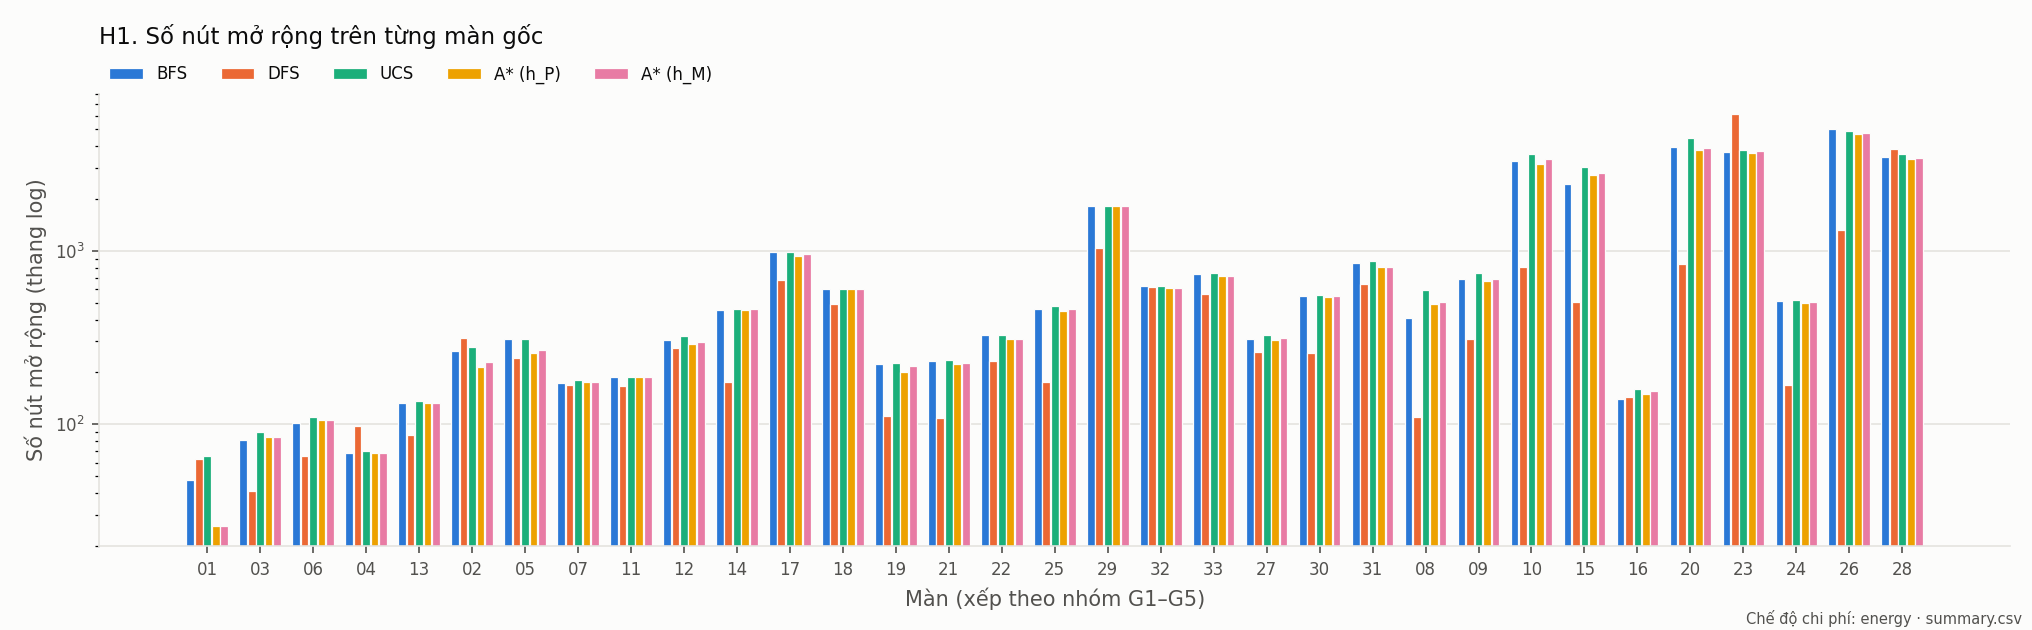
\includegraphics[width=0.86\linewidth,height=\textheight,keepaspectratio,alt={Hình 5.1}]{hinh/h5-1-so-nut-mo-rong.png}
\caption{Hình 5.1. Số nút mở rộng trên từng màn gốc, thang log. DFS mở rộng ít nút nhất ở 26/33 màn. DFS mở rộng nhiều hơn BFS ở 6 màn: 01, 02, 04, 16, 23, 28.}
\end{figure}

\begin{figure}
\centering
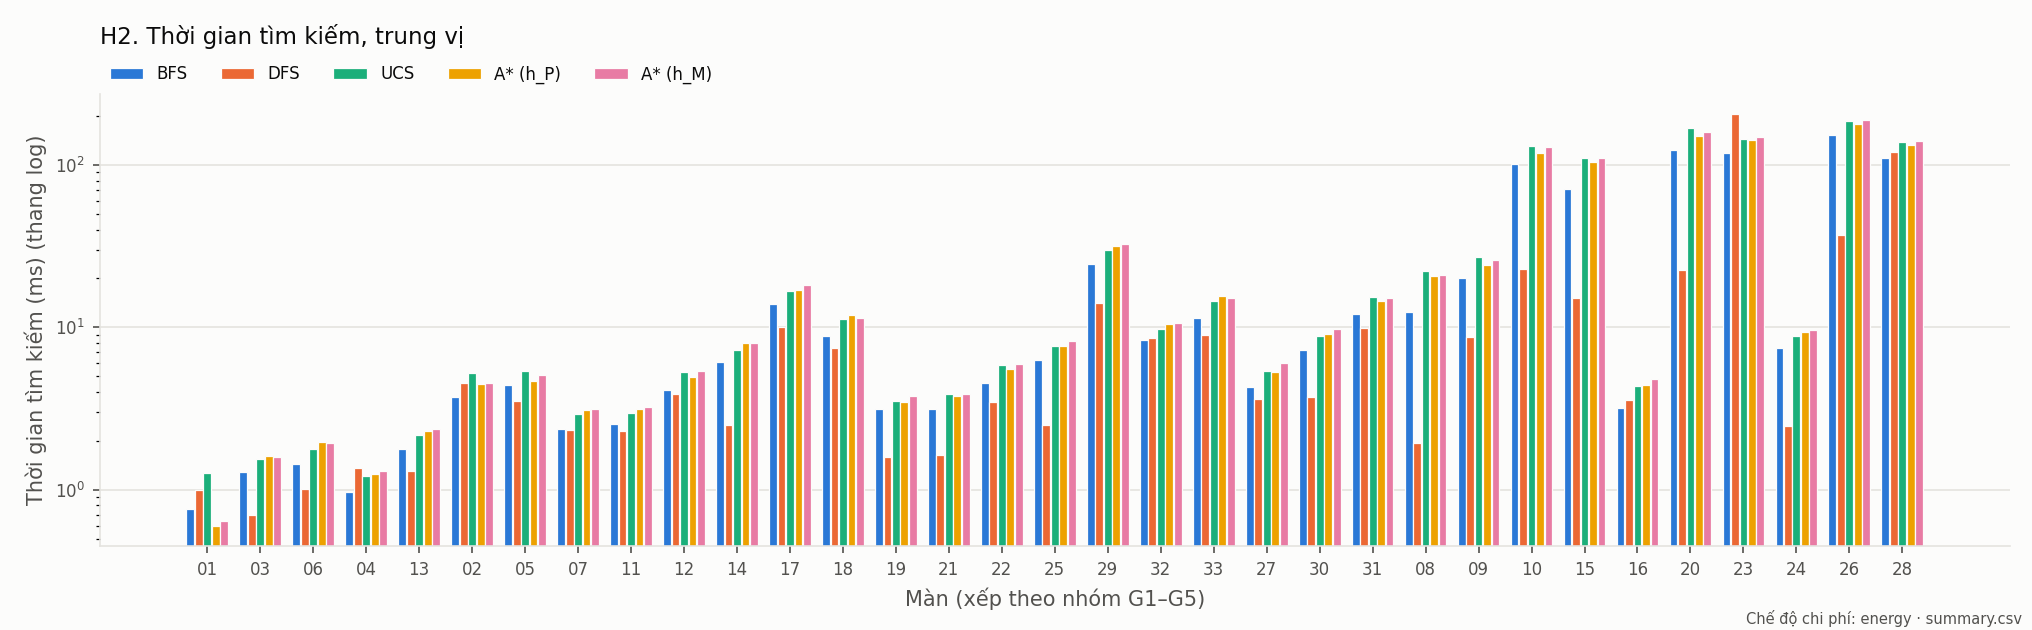
\includegraphics[width=0.86\linewidth,height=\textheight,keepaspectratio,alt={Hình 5.2}]{hinh/h5-2-thoi-gian.png}
\caption{Hình 5.2. Thời gian tìm kiếm trên từng màn gốc. Thời gian đi theo số nút mở rộng: tương quan hạng Spearman giữa hai cột trên 165 cặp (màn, thuật toán) là 0,978.}
\end{figure}

\begin{figure}
\centering
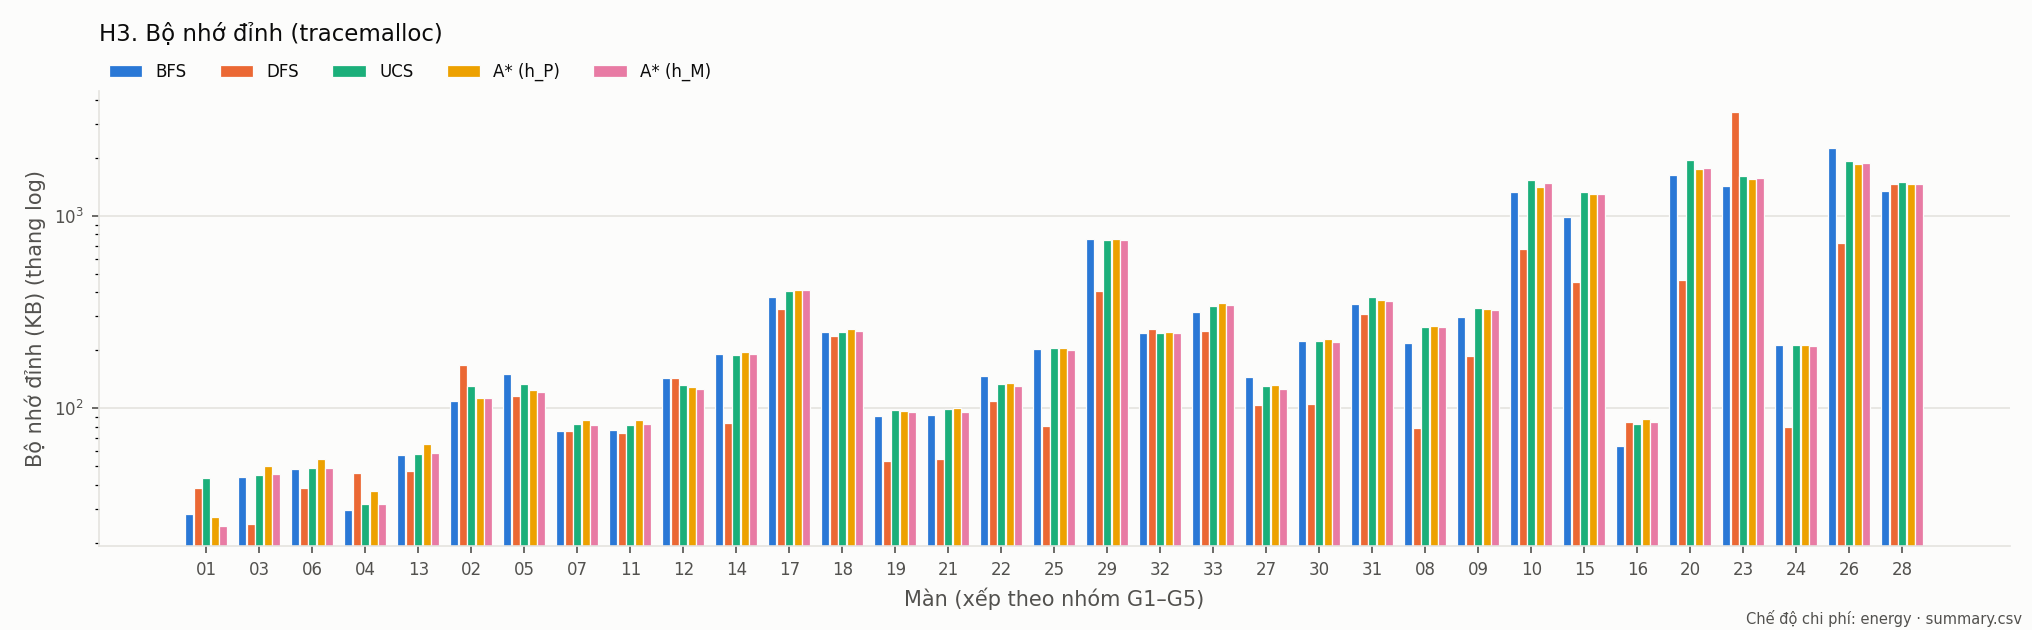
\includegraphics[width=0.86\linewidth,height=\textheight,keepaspectratio,alt={Hình 5.3}]{hinh/h5-3-bo-nho.png}
\caption{Hình 5.3. Bộ nhớ đỉnh trên từng màn gốc. Bộ nhớ đi theo số trạng thái đã thăm: tương quan hạng Spearman 0,997.}
\end{figure}

\begin{figure}
\centering
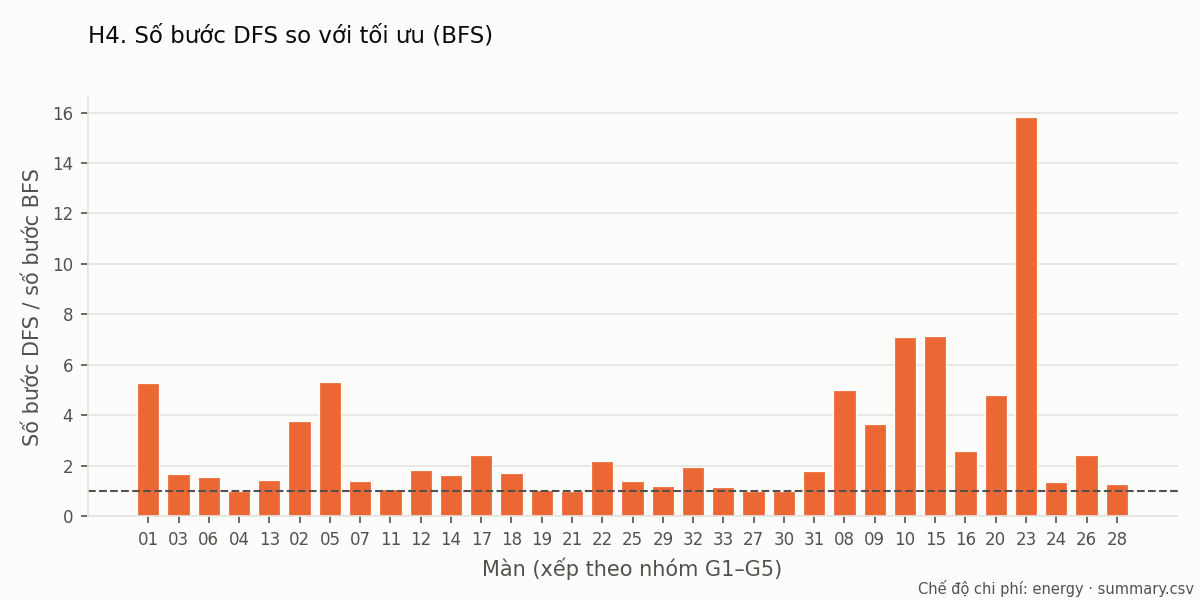
\includegraphics[width=0.86\linewidth,height=\textheight,keepaspectratio,alt={Hình 5.4}]{hinh/h5-4-dfs-so-voi-toi-uu.png}
\caption{Hình 5.4. Số bước của DFS chia cho số bước tối ưu. Trung vị theo màn là 1,73; lớn nhất 15,83 ở màn 23. DFS ra đúng số bước tối ưu ở 3 màn: 04, 21, 27.}
\end{figure}

\begin{figure}
\centering
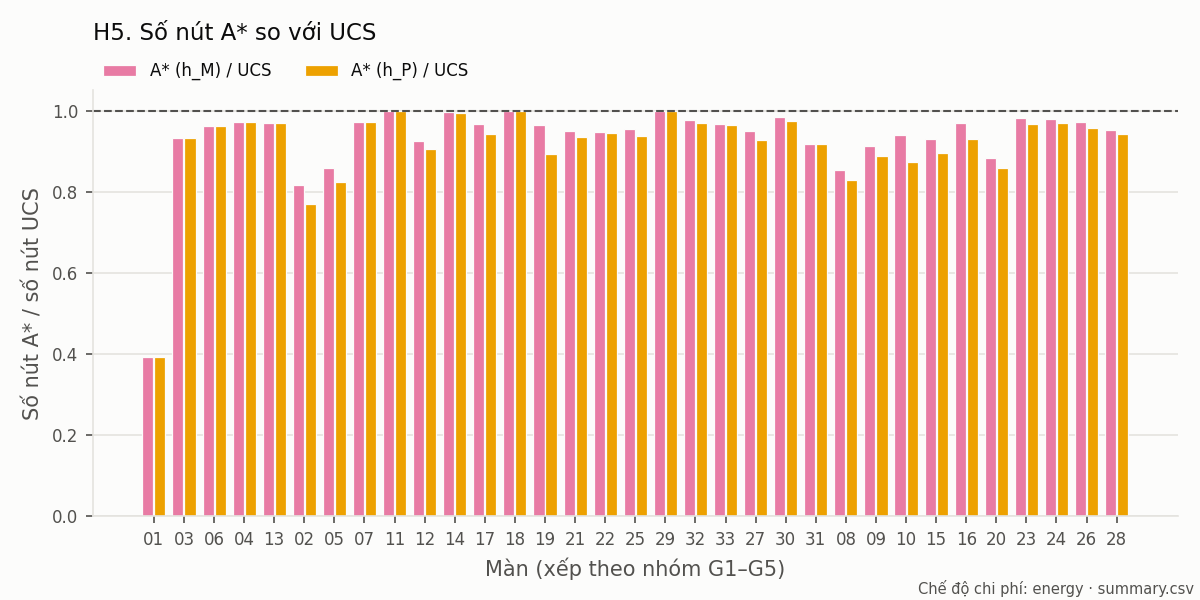
\includegraphics[width=0.86\linewidth,height=\textheight,keepaspectratio,alt={Hình 5.5}]{hinh/h5-5-astar-so-voi-ucs.png}
\caption{Hình 5.5. Số nút của A}
\end{figure}

\begin{figure}
\centering
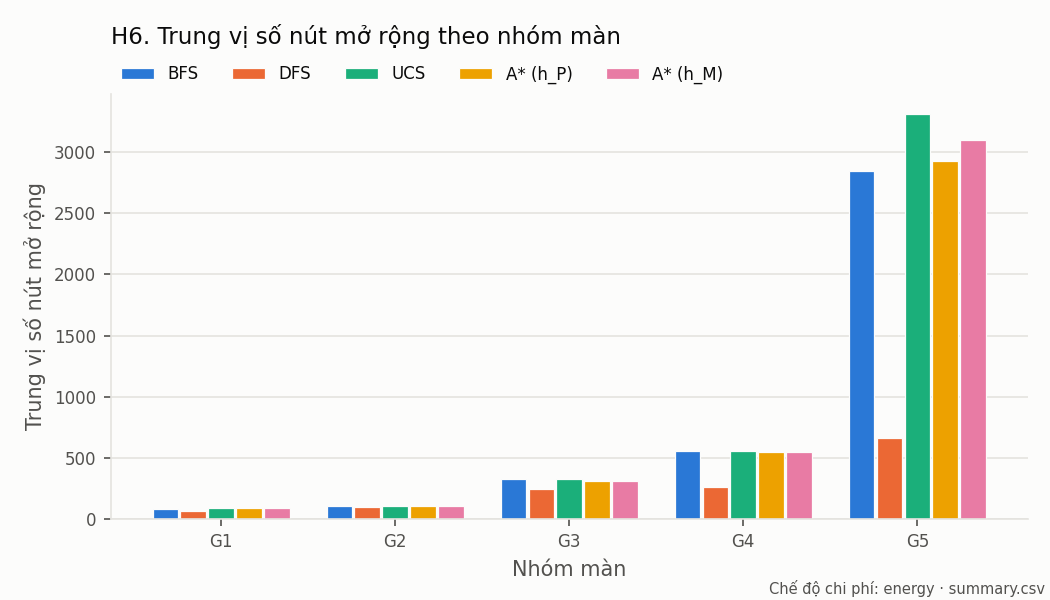
\includegraphics[width=0.86\linewidth,height=\textheight,keepaspectratio,alt={Hình 5.6}]{hinh/h5-6-theo-nhom.png}
\caption{Hình 5.6. Trung vị số nút mở rộng theo nhóm, thang tuyến tính. Nhóm G5 (công tắc tách) lớn nhất ở mọi thuật toán: so với G4, gấp 5,2 lần với BFS, 5,9 lần với UCS, 5,3 lần với A}
\end{figure}

\begin{figure}
\centering
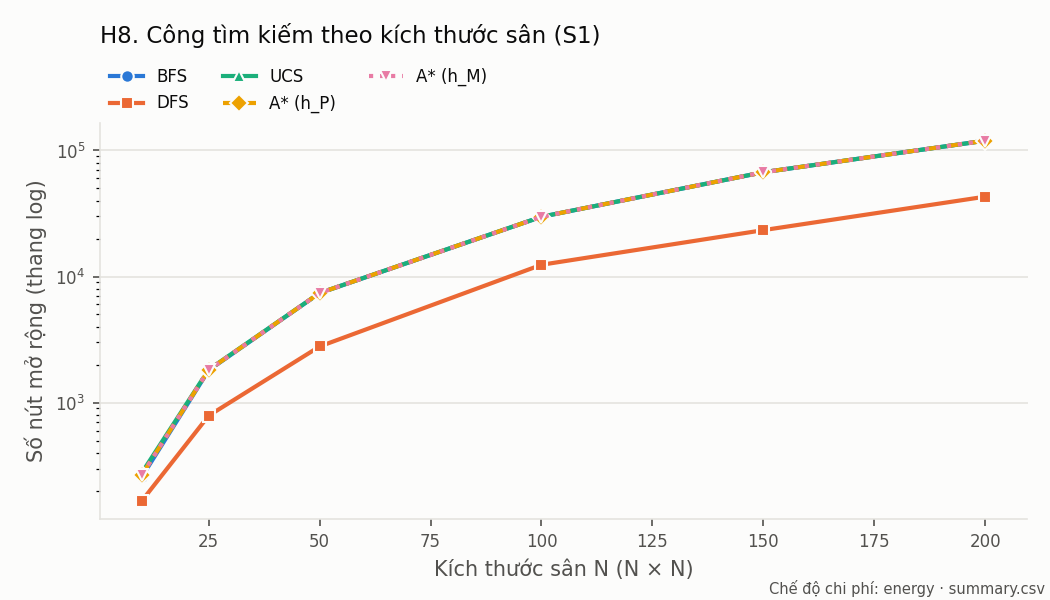
\includegraphics[width=0.86\linewidth,height=\textheight,keepaspectratio,alt={Hình 5.7}]{hinh/h5-7-san-trong-s1.png}
\caption{Hình 5.7. Số nút mở rộng theo kích thước sân N (S1). BFS mở rộng xấp xỉ \(3N^2\) nút (2,59 \(N^2\) ở N = 10, 2,99 \(N^2\) ở N = 200). Đường của UCS và A}
\end{figure}

\begin{figure}
\centering
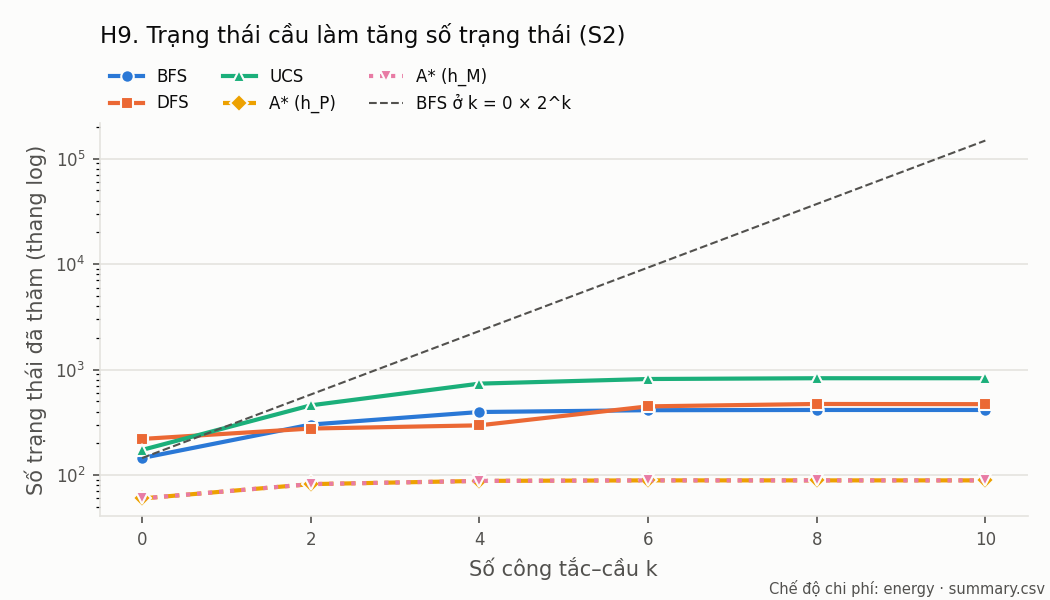
\includegraphics[width=0.86\linewidth,height=\textheight,keepaspectratio,alt={Hình 5.8}]{hinh/h5-8-cau-s2.png}
\caption{Hình 5.8. Số trạng thái đã thăm theo số công tắc k (S2); đường nét đứt là số trạng thái BFS thăm ở k = 0, nhân \(2^k\). Số trạng thái thực tế đi ngang từ k = 6 và còn xa đường \(2^k\).}
\end{figure}

\textbf{Bộ màn tự sinh.} Số liệu chọn lọc từ \texttt{summary.\allowbreak{}csv}:

{\def\LTcaptype{none} % do not increment counter
\begin{longtable}[]{@{}
  >{\raggedright\arraybackslash}p{(\linewidth - 14\tabcolsep) * \real{0.1111}}
  >{\raggedright\arraybackslash}p{(\linewidth - 14\tabcolsep) * \real{0.1222}}
  >{\raggedright\arraybackslash}p{(\linewidth - 14\tabcolsep) * \real{0.1806}}
  >{\raggedright\arraybackslash}p{(\linewidth - 14\tabcolsep) * \real{0.1000}}
  >{\raggedright\arraybackslash}p{(\linewidth - 14\tabcolsep) * \real{0.1083}}
  >{\raggedright\arraybackslash}p{(\linewidth - 14\tabcolsep) * \real{0.1139}}
  >{\raggedright\arraybackslash}p{(\linewidth - 14\tabcolsep) * \real{0.1278}}
  >{\raggedright\arraybackslash}p{(\linewidth - 14\tabcolsep) * \real{0.1361}}@{}}
\toprule\noalign{}
\begin{minipage}[b]{\linewidth}\raggedright
\textbf{Màn}
\end{minipage} & \begin{minipage}[b]{\linewidth}\raggedright
\textbf{Thuật toán}
\end{minipage} & \begin{minipage}[b]{\linewidth}\raggedright
\textbf{Kết quả}
\end{minipage} & \begin{minipage}[b]{\linewidth}\raggedright
\textbf{Số bước}
\end{minipage} & \begin{minipage}[b]{\linewidth}\raggedright
\textbf{Nút mở rộng}
\end{minipage} & \begin{minipage}[b]{\linewidth}\raggedright
\textbf{Trạng thái đã thăm}
\end{minipage} & \begin{minipage}[b]{\linewidth}\raggedright
\textbf{Thời gian (ms)}
\end{minipage} & \begin{minipage}[b]{\linewidth}\raggedright
\textbf{Bộ nhớ (KB)}
\end{minipage} \\
\midrule\noalign{}
\endhead
\bottomrule\noalign{}
\endlastfoot
\texttt{s1\_\allowbreak{}200} & BFS & solved & 266 & 119 589 & 119 598 & 2 195,64 & 44 736,48 \\
\texttt{s1\_\allowbreak{}200} & DFS & solved & 35 287 & 43 013 & 98 095 & 914,64 & 39 080,73 \\
\texttt{s1\_\allowbreak{}200} & UCS & solved & 266 & 119 599 & 119 600 & 3 357,73 & 50 718,93 \\
\texttt{s1\_\allowbreak{}200} & A* (\(h_P\)) & solved & 266 & 119 597 & 119 600 & 3 439,23 & 55 926,54 \\
\texttt{s2\_\allowbreak{}00} & BFS & solved & 6 & 95 & 145 & 1,52 & 61,27 \\
\texttt{s2\_\allowbreak{}10} & BFS & solved & 6 & 197 & 414 & 3,41 & 200,24 \\
\texttt{s2\_\allowbreak{}10} & A* (\(h_P\)) & solved & 6 & 30 & 89 & 0,85 & 62,39 \\
\texttt{s3\_\allowbreak{}50} & BFS & no\_solution & & 7 400 & 7 400 & 122,87 & 3 004,41 \\
\texttt{s3\_\allowbreak{}50} & DFS & no\_solution & & 7 400 & 7 400 & 123,51 & 3 003,11 \\
\texttt{s3\_\allowbreak{}50} & UCS & no\_solution & & 7 400 & 7 400 & 164,30 & 3 081,45 \\
\texttt{s3\_\allowbreak{}50} & A* (\(h_P\)) & no\_solution & & 0 & 1 & 0,01 & 13,98 \\
\texttt{s3\_\allowbreak{}50} & A* (\(h_M\)) & no\_solution & & 7 400 & 7 400 & 184,18 & 3 107,64 \\
\end{longtable}
}

\textbf{Timeout và không có lời giải.}

\begin{itemize}
\tightlist
\item
  Không cặp nào hết giờ (60 giây). Cặp chạy lâu nhất là A* (\(h_P\)) trên \texttt{s1\_\allowbreak{}200}: 3 439,23 ms thời gian tìm kiếm.
\item
  10 cặp \texttt{no\_\allowbreak{}solution} đều ở S3, đúng như thiết kế.
\item
  Không có dòng \texttt{invalid} hay lỗi (K1).
\end{itemize}

\textbf{Trước và sau khi sửa chi phí bước tách.} Lần đo trước, trên commit \texttt{cd93624}, tính bước tách 1,0. Dữ liệu của lần đo đó vẫn giữ ở \texttt{Source/\allowbreak{}experiments/\allowbreak{}benchmark-\allowbreak{}2026-\allowbreak{}10-\allowbreak{}31-\allowbreak{}cd93624/\allowbreak{}}, kèm ghi chú đã bị thay thế. So hai \texttt{summary.\allowbreak{}csv} bằng \texttt{compare\_\allowbreak{}runs.\allowbreak{}py} (\texttt{so-\allowbreak{}sanh-\allowbreak{}voi-\allowbreak{}cd93624.\allowbreak{}txt}):

\begin{itemize}
\tightlist
\item
  50 cặp khác nhau, đúng bằng 10 màn G5 × 5 cấu hình; 185 cặp còn lại trùng hẳn ở mọi số đếm, tổng chi phí và bộ nhớ.
\item
  Số bước không đổi ở mọi cặp.
\item
  BFS và DFS chỉ khác ở tổng chi phí, vì hai thuật toán không dùng chi phí khi chọn nút. Mỗi bước tách trên lời giải đắt thêm 0,62.
\item
  UCS và A* khác thêm ở số đếm, vì chi phí bước tách đổi thứ tự lấy nút ra khỏi hàng đợi.
\end{itemize}

\begin{longtable}[]{@{}
  >{\raggedright\arraybackslash}p{(\linewidth - 10\tabcolsep) * \real{0.0694}}
  >{\raggedright\arraybackslash}p{(\linewidth - 10\tabcolsep) * \real{0.2288}}
  >{\raggedright\arraybackslash}p{(\linewidth - 10\tabcolsep) * \real{0.0972}}
  >{\raggedright\arraybackslash}p{(\linewidth - 10\tabcolsep) * \real{0.2010}}
  >{\raggedright\arraybackslash}p{(\linewidth - 10\tabcolsep) * \real{0.2018}}
  >{\raggedright\arraybackslash}p{(\linewidth - 10\tabcolsep) * \real{0.2018}}@{}}
\caption{\textbf{Bảng 5.10.} Nhóm G5 trước (\texttt{cd93624}, bước tách 1,0) và sau (\texttt{0a35afd}, bước tách 1,62) khi sửa.}\tabularnewline
\toprule\noalign{}
\begin{minipage}[b]{\linewidth}\raggedright
\textbf{Màn}
\end{minipage} & \begin{minipage}[b]{\linewidth}\raggedright
\textbf{Tổng chi phí tối ưu (UCS)}
\end{minipage} & \begin{minipage}[b]{\linewidth}\raggedright
\textbf{Chênh}
\end{minipage} & \begin{minipage}[b]{\linewidth}\raggedright
\textbf{Nút mở rộng UCS}
\end{minipage} & \begin{minipage}[b]{\linewidth}\raggedright
\textbf{Nút A* (\(h_P\))}
\end{minipage} & \begin{minipage}[b]{\linewidth}\raggedright
\textbf{Nút A* (\(h_M\))}
\end{minipage} \\
\midrule\noalign{}
\endfirsthead
\toprule\noalign{}
\begin{minipage}[b]{\linewidth}\raggedright
\textbf{Màn}
\end{minipage} & \begin{minipage}[b]{\linewidth}\raggedright
\textbf{Tổng chi phí tối ưu (UCS)}
\end{minipage} & \begin{minipage}[b]{\linewidth}\raggedright
\textbf{Chênh}
\end{minipage} & \begin{minipage}[b]{\linewidth}\raggedright
\textbf{Nút mở rộng UCS}
\end{minipage} & \begin{minipage}[b]{\linewidth}\raggedright
\textbf{Nút A* (\(h_P\))}
\end{minipage} & \begin{minipage}[b]{\linewidth}\raggedright
\textbf{Nút A* (\(h_M\))}
\end{minipage} \\
\midrule\noalign{}
\endhead
\bottomrule\noalign{}
\endlastfoot
08 & 11,98 → 12,60 & +0,62 & 594 → 594 & 492 → 492 & 507 → 508 \\
09 & 28,68 → 29,30 & +0,62 & 749 → 749 & 666 → 666 & 684 → 684 \\
10 & 66,82 → 67,44 & +0,62 & 3 611 → 3 505 & 3 153 → 3 086 & 3 391 → 3 356 \\
15 & 68,22 → 68,84 & +0,62 & 3 031 → 3 031 & 2 715 → 2 715 & 2 821 → 2 821 \\
16 & 33,88 → 38,22 & +4,34 & 160 → 168 & 149 → 160 & 155 → 160 \\
20 & 70,06 → 70,68 & +0,62 & 4 437 → 4 438 & 3 810 → 3 813 & 3 915 → 3 917 \\
23 & 99,96 → 100,58 & +0,62 & 3 804 → 3 755 & 3 682 → 3 682 & 3 737 → 3 711 \\
24 & 75,69 → 76,31 & +0,62 & 518 → 523 & 502 → 504 & 508 → 511 \\
26 & 124,26 → 125,50 & +1,24 & 4 910 → 4 910 & 4 704 → 4 704 & 4 778 → 4 778 \\
28 & 127,35 → 127,97 & +0,62 & 3 603 → 3 603 & 3 397 → 3 397 & 3 434 → 3 434 \\
\end{longtable}

Mức chênh tổng chi phí là bội của 0,62: lời giải tối ưu của màn 16 có 7 bước tách, của màn 26 có 2, các màn còn lại có 1. Các kết luận ở mục 5.5 không đổi; chỉ các con số của G5 và các tổng có chứa G5 đổi theo. Hai thay đổi lớn nhất:

\begin{itemize}
\tightlist
\item
  trung vị G5 của UCS giảm từ 3 317 xuống 3 268 nút, của A* (\(h_P\)) từ 2 934 xuống 2 900 (Bảng 5.5);
\item
  ở màn 16, A* (\(h_P\)) và A* (\(h_M\)) nay cùng mở rộng 160 nút, nên số màn \(h_P\) bằng \(h_M\) tăng từ 10 lên 11.
\end{itemize}

Thời gian ở mọi cặp đều đổi giữa hai lần đo, kể cả ở 185 cặp không bị ảnh hưởng, nên phần lệch thời gian không dùng để đánh giá việc sửa (xem phần hạn chế ở mục 5.5).

\subsection{5.4. Nhận xét từng thuật toán}

Mục này nhận xét kết quả của từng thuật toán: BFS (5.4.1), DFS (5.4.2), UCS (5.4.3) và A* (5.4.4). Mỗi mục trả lời các câu hỏi riêng của thuật toán đó theo ba bước: quan sát, giải thích, ý nghĩa.

\subsubsection{5.4.1. Nhận xét kết quả BFS}

Số liệu lấy từ lần đo ở mục 5.3 (Bảng 5.2), với hàm chi phí ở Bảng 3.3.1; thời gian là trung vị của 5 lần đo. Số bước và số nút của BFS và DFS là tất định. Số nút của UCS và A* chỉ đổi khi đổi hàm chi phí. Thời gian và bộ nhớ phụ thuộc máy, nên chỉ nên so tỉ lệ giữa các thuật toán.

\textbf{Lời giải của BFS có tối ưu không?} Theo số bước thì có: BFS ra đúng số bước tối ưu tham khảo ở 33/33 màn gốc, và lời giải nào phát lại trên engine cũng tới đích. Theo chi phí thì không bảo đảm. BFS có tổng chi phí bằng UCS ở 31/33 màn; hai màn còn lại là màn 17 (140,42 so với 140,10) và màn 23 (101,58 so với 100,58). Ở hai màn này, nhiều đường có cùng số bước ít nhất. BFS lấy đường đi trước theo thứ tự U, D, L, R, còn UCS chọn đường rẻ hơn trong số đó. Ở màn 17, đường của UCS dựng khối đứng ít hơn một lần và thay bằng hai lần lăn khối nằm. Ở màn 23, đường của UCS có ít hơn hai bước đặt khối lên ô dễ vỡ (21 so với 23 bước). Chênh lệch không quá 1 \%, vì mọi chi phí bước đều nằm trong khoảng 1,10 đến 1,71, nên đường ít bước nhất gần như luôn là đường rẻ nhất.

\textbf{BFS mở rộng bao nhiêu nút so với các thuật toán khác?} Bảng 5.5 cho trung vị số nút mở rộng theo nhóm màn.

\begin{itemize}
\tightlist
\item
  BFS mở rộng ít nút hơn UCS ở 29/33 màn (tổng 33 459 so với 35 281). Có hai lý do. Thứ nhất, BFS kiểm tra đích khi sinh nút nên dừng sớm hơn một lớp; UCS phải chờ tới khi lấy đích ra khỏi hàng đợi. Thứ hai, với chi phí không đồng nhất, UCS phải mở rộng mọi trạng thái rẻ hơn lời giải tối ưu, kể cả những trạng thái nhiều bước hơn nhưng rẻ hơn.
\item
  A* với \(h_P\) mở rộng ít nút hơn BFS ở 21/33 màn, bằng BFS ở 5 màn và nhiều hơn ở 7 màn. Tính trên tổng, A* chỉ ít hơn khoảng 2 \% (32 712 so với 33 459). Heuristic ⌈Φ/2⌉ là cận dưới của số bước, trong khi mỗi bước tốn 1,1 đến 1,7, nên heuristic chỉ cắt được một phần nhỏ không gian (mục 5.4.4).
\item
  DFS mở rộng ít nút nhất (tổng 21 041) nhưng lời giải dài hơn nhiều (mục 5.4.2). Số nút ít của DFS không có nghĩa là DFS tốt hơn: DFS dừng ở đích đầu tiên trên nhánh đang đi, BFS phải bảo đảm không còn lời giải nào ngắn hơn.
\end{itemize}

\textbf{Công tìm kiếm của BFS dồn vào đâu?} Vào các màn có công tắc tách. Trung vị số nút mở rộng của nhóm G5 (2 851) gấp gần 9 lần nhóm G3 (325), dù lời giải ở G3 thường dài hơn (trung vị 65 bước, so với 57 bước ở G5). Như mục 2.3 đã chỉ ra, trạng thái đã tách chiếm 90--95 \% không gian ở các màn này, và hệ số phân nhánh tăng từ khoảng 2 lên khoảng 5 (mục 3.1.4). Cầu làm không gian lớn lên ít hơn nhiều: số cấu hình cầu tới được ở 33 màn nhiều nhất là 21.

\textbf{Thời gian và bộ nhớ.} Trên 33 màn gốc, tổng thời gian tìm kiếm của BFS là 898,2 ms, thấp hơn UCS (1 163,2 ms) và A* (1 130,6 ms với \(h_P\), 1 193,3 ms với \(h_M\)). Thời gian trung vị cho mỗi nút mở rộng của BFS (15,1 µs) gần bằng DFS (15,8 µs) và thấp hơn UCS (18,6 µs) và A* (19,2 µs với \(h_P\), 19,9 µs với \(h_M\)). Hàng đợi \texttt{deque} thêm và lấy với chi phí \(O(1)\), còn hàng đợi ưu tiên \texttt{heapq} tốn \(O(\log n)\) mỗi lần, cộng thêm phần tính chi phí và heuristic. Trung vị bộ nhớ đỉnh của BFS ở nhóm G5 là 1 160,2 KB, ít hơn UCS (1 418,9 KB) vì BFS thăm ít trạng thái hơn (Bảng 5.7). Như mục 3.1.4 đã nêu, bộ nhớ chủ yếu nằm ở tập đã thăm và bảng cha.

\textbf{Khi bàn lớn dần (bộ S1).} S1 là sân trống N × N, xuất phát ở góc trên trái và đích ở góc dưới phải (Bảng 5.4.1).

\begin{longtable}[]{@{}
  >{\raggedright\arraybackslash}p{(\linewidth - 12\tabcolsep) * \real{0.1131}}
  >{\raggedright\arraybackslash}p{(\linewidth - 12\tabcolsep) * \real{0.1270}}
  >{\raggedright\arraybackslash}p{(\linewidth - 12\tabcolsep) * \real{0.1687}}
  >{\raggedright\arraybackslash}p{(\linewidth - 12\tabcolsep) * \real{0.1687}}
  >{\raggedright\arraybackslash}p{(\linewidth - 12\tabcolsep) * \real{0.1270}}
  >{\raggedright\arraybackslash}p{(\linewidth - 12\tabcolsep) * \real{0.1270}}
  >{\raggedright\arraybackslash}p{(\linewidth - 12\tabcolsep) * \real{0.1687}}@{}}
\caption{\textbf{Bảng 5.4.1.} BFS trên bộ sân trống S1.}\tabularnewline
\toprule\noalign{}
\begin{minipage}[b]{\linewidth}\raggedright
\textbf{N}
\end{minipage} & \begin{minipage}[b]{\linewidth}\raggedright
\textbf{Số bước}
\end{minipage} & \begin{minipage}[b]{\linewidth}\raggedright
\textbf{Nút mở rộng}
\end{minipage} & \begin{minipage}[b]{\linewidth}\raggedright
\textbf{Trạng thái đã thăm}
\end{minipage} & \begin{minipage}[b]{\linewidth}\raggedright
\textbf{Biên lớn nhất}
\end{minipage} & \begin{minipage}[b]{\linewidth}\raggedright
\textbf{Bộ nhớ đỉnh (MB)}
\end{minipage} & \begin{minipage}[b]{\linewidth}\raggedright
\textbf{Thời gian (ms)}
\end{minipage} \\
\midrule\noalign{}
\endfirsthead
\toprule\noalign{}
\begin{minipage}[b]{\linewidth}\raggedright
\textbf{N}
\end{minipage} & \begin{minipage}[b]{\linewidth}\raggedright
\textbf{Số bước}
\end{minipage} & \begin{minipage}[b]{\linewidth}\raggedright
\textbf{Nút mở rộng}
\end{minipage} & \begin{minipage}[b]{\linewidth}\raggedright
\textbf{Trạng thái đã thăm}
\end{minipage} & \begin{minipage}[b]{\linewidth}\raggedright
\textbf{Biên lớn nhất}
\end{minipage} & \begin{minipage}[b]{\linewidth}\raggedright
\textbf{Bộ nhớ đỉnh (MB)}
\end{minipage} & \begin{minipage}[b]{\linewidth}\raggedright
\textbf{Thời gian (ms)}
\end{minipage} \\
\midrule\noalign{}
\endhead
\bottomrule\noalign{}
\endlastfoot
10 & 12 & 259 & 273 & 53 & 0,10 & 4,1 \\
25 & 32 & 1 804 & 1 818 & 122 & 0,73 & 30,9 \\
50 & 66 & 7 389 & 7 398 & 235 & 2,9 & 122,9 \\
100 & 132 & 29 779 & 29 793 & 472 & 11,9 & 537,7 \\
150 & 200 & 67 197 & 67 200 & 703 & 24,0 & 1 160,7 \\
200 & 266 & 119 589 & 119 598 & 935 & 43,7 & 2 195,6 \\
\end{longtable}

Đích nằm ở góc xa nhất, nên BFS thăm gần như toàn bộ \(3N^2 - 2N\) trạng thái của sân: ví dụ với N = 200 là 119 598 trên 119 600. Khi N tăng gấp đôi từ 100 lên 200, số nút tăng 4,0 lần, thời gian 4,1 lần, bộ nhớ 3,7 lần, đúng với bậc \(O(N^2)\) của số trạng thái. Biên lớn nhất chỉ tăng tuyến tính theo N (từ 53 lên 935), vì biên của BFS là một ``đường sóng'' lan dần ra từ góc xuất phát. Một lần nữa, bộ nhớ nằm ở tập đã thăm chứ không ở biên.

\textbf{Khi không có lời giải (bộ S3).} BFS duyệt hết mọi trạng thái tới được rồi trả \texttt{no\_\allowbreak{}solution}: 280 nút với vùng 10 × 10 và 7 400 nút với vùng 50 × 50. DFS, UCS và A* với \(h_M\) mở rộng đúng số nút đó, vì thuật toán nào cũng phải duyệt hết mới kết luận được. Chỉ A* với \(h_P\) kết luận ngay mà không mở rộng nút nào, vì \(h_P\) phát hiện ô đích không nối được với vùng xuất phát (mục 3.4).

\textbf{Khi có thêm công tắc (bộ S2).} Số trạng thái BFS đã thăm tăng từ 145 (k = 0) lên 414 (k = 10) và gần như không đổi từ k = 6. Mức tăng nhỏ hơn rất nhiều so với \(2^k\), vì BFS gặp đích ở độ sâu 6, trước khi kịp đi bấm phần lớn các công tắc. Như vậy, cầu chỉ làm tăng công tìm kiếm khi lời giải thật sự phải đi qua các công tắc.

\textbf{Ý nghĩa.} BFS là lựa chọn tốt khi cần lời giải ít bước nhất, ví dụ để gợi ý nước đi cho người chơi. BFS đơn giản, có chi phí mỗi nút thấp nhất trong bốn thuật toán, và trên 33 màn gốc chạy nhanh hơn cả UCS lẫn A\emph{. BFS không phù hợp khi các bước có chi phí khác nhau, vì nó bỏ qua chi phí (màn 17, 23). Trên không gian lớn, BFS cũng không phù hợp vì tốn bộ nhớ tỉ lệ với số trạng thái đã thăm; khi đó A} với heuristic mạnh hơn sẽ cắt được nhiều nút hơn.

\subsubsection{5.4.2. Nhận xét kết quả DFS}

Số liệu lấy từ lần đo ở mục 5.3. Số bước, số đếm, thời gian và bộ nhớ của DFS không phụ thuộc hàm chi phí, vì DFS không dùng chi phí khi chọn nút; chỉ cột tổng chi phí phụ thuộc. Mục này trả lời bốn câu hỏi, mỗi câu theo ba bước: quan sát, giải thích, ý nghĩa.

\textbf{DFS nhanh hay chậm so với BFS?}

\begin{itemize}
\tightlist
\item
  \emph{Quan sát:}

  \begin{itemize}
  \tightlist
  \item
    Trung vị số nút mở rộng và thời gian tìm kiếm của DFS nhỏ hơn BFS ở cả 5 nhóm (Bảng 5.5, 5.6). Ví dụ ở G5: DFS 658 nút, 19,32 ms; BFS 2 851 nút, 92,16 ms.
  \item
    Theo từng màn, DFS mở rộng ít nút nhất trong năm cấu hình ở 26/33 màn, và nhanh hơn BFS ở 26/33 màn.
  \item
    Có 6 màn DFS mở rộng nhiều hơn BFS: 01, 02, 04, 16, 23, 28 (Hình 5.1).
  \item
    Tổng thời gian tìm kiếm trên 33 màn: DFS 565,1 ms, BFS 898,2 ms.
  \end{itemize}
\item
  \emph{Giải thích:} DFS dừng ngay khi nhánh nó đang đi chạm đích. Nếu nhánh đầu tiên (thử lên trước, rồi xuống, trái, phải) tình cờ đi về phía đích, DFS mở rộng ít nút hơn BFS. Nếu không, DFS đi sâu vào các vùng xa đích, và có thể duyệt gần hết không gian trạng thái trước khi gặp đích; đó là trường hợp của 6 màn trên. BFS và DFS có cùng chi phí cho mỗi nút: một lần lấy ra, gọi hàm chuyển cho 4 hoặc 8 hành động, và tra tập đã thăm. Vì vậy chênh lệch thời gian chủ yếu đến từ chênh lệch số nút (Hình 5.2).
\end{itemize}

\textbf{Lời giải dài gấp bao nhiêu lần tối ưu?}

\begin{itemize}
\tightlist
\item
  \emph{Quan sát} (Hình 5.4, Bảng 5.8):

  \begin{itemize}
  \tightlist
  \item
    Số bước DFS chia số bước tối ưu: trung vị 1,73 theo màn, trung bình 288,3 \%, lớn nhất 15,83 lần ở màn 23.
  \item
    DFS ra đúng số bước tối ưu ở 3 màn: 04, 21, 27. Ví dụ ở màn 1: DFS đi 37 bước, so với 7 bước tối ưu (Bảng 3.2.1).
  \item
    Ở sân trống \texttt{s1\_\allowbreak{}200}: DFS đi 35 287 bước, so với 266 bước tối ưu.
  \item
    Tổng chi phí của DFS lớn hơn UCS ở 30/33 màn; tỉ lệ trung vị 1,72, lớn nhất 15,17.
  \end{itemize}
\item
  \emph{Giải thích:} DFS không so sánh độ dài giữa các nhánh. Mỗi trạng thái được gán cho cha đầu tiên sinh ra nó, nên lời giải là nhánh DFS đã đi, kể cả các đoạn đi vòng. Với bàn rộng và ít vật cản, đoạn đi vòng càng dài (nhóm S1). Mỗi bước tốn ít nhất 1,10, nên lời giải nhiều bước hơn cũng tốn chi phí hơn; tỉ lệ chi phí (trung vị 1,72) gần bằng tỉ lệ số bước (1,73).
\end{itemize}

\textbf{Thứ tự hành động ảnh hưởng ra sao?}

Kết quả của DFS phụ thuộc hoàn toàn vào thứ tự U, D, L, R. Thứ tự này cố định và giống nhau ở mọi thuật toán (mục 2.4), nên mọi con số của DFS chỉ đúng với thứ tự đó.

Ví dụ ở các màn S1 (xuất phát ở góc trên trái, đích ở góc dưới phải):

\begin{itemize}
\tightlist
\item
  ở nước đầu, ``lên'' và ``trái'' làm khối rơi khỏi bàn, nên DFS đi ``xuống'' trước, đúng hướng đích;
\item
  nhưng ở mọi trạng thái sau đó mà ``lên'' hợp lệ, DFS đều thử ``lên'' trước;
\item
  vì vậy, khi đã xuống tới mép dưới, khối lại lăn ngược lên, và lời giải đi zíc zắc qua bàn thay vì đi thẳng tới đích.
\end{itemize}

\textbf{Nhóm chưa đo} DFS với các thứ tự hành động khác. Biên độ thay đổi theo thứ tự là một hạn chế của thực nghiệm này.

\textbf{Ở màn không có lời giải (S3), DFS dừng thế nào?}

DFS của nhóm có tập đã thăm, nên mỗi trạng thái được mở rộng nhiều nhất một lần. Ở màn không có lời giải, DFS duyệt hết các trạng thái tới được từ trạng thái đầu rồi trả \texttt{no\_\allowbreak{}solution}. Nó không lặp vô hạn, và không cần timeout để dừng (mục 3.2.5; test \texttt{test\_\allowbreak{}no\_\allowbreak{}solution\_\allowbreak{}when\_\allowbreak{}gap\_\allowbreak{}is\_\allowbreak{}two\_\allowbreak{}tiles}).

\emph{Quan sát}, đúng như dự đoán:

{\def\LTcaptype{none} % do not increment counter
\begin{longtable}[]{@{}
  >{\raggedright\arraybackslash}p{(\linewidth - 10\tabcolsep) * \real{0.1435}}
  >{\raggedright\arraybackslash}p{(\linewidth - 10\tabcolsep) * \real{0.1435}}
  >{\raggedright\arraybackslash}p{(\linewidth - 10\tabcolsep) * \real{0.1435}}
  >{\raggedright\arraybackslash}p{(\linewidth - 10\tabcolsep) * \real{0.1435}}
  >{\raggedright\arraybackslash}p{(\linewidth - 10\tabcolsep) * \real{0.1991}}
  >{\raggedright\arraybackslash}p{(\linewidth - 10\tabcolsep) * \real{0.2269}}@{}}
\toprule\noalign{}
\begin{minipage}[b]{\linewidth}\raggedright
\textbf{Màn}
\end{minipage} & \begin{minipage}[b]{\linewidth}\raggedright
\textbf{Thuật toán}
\end{minipage} & \begin{minipage}[b]{\linewidth}\raggedright
\textbf{Nút mở rộng}
\end{minipage} & \begin{minipage}[b]{\linewidth}\raggedright
\textbf{Trạng thái đã thăm}
\end{minipage} & \begin{minipage}[b]{\linewidth}\raggedright
\textbf{Thời gian}
\end{minipage} & \begin{minipage}[b]{\linewidth}\raggedright
\textbf{Bộ nhớ}
\end{minipage} \\
\midrule\noalign{}
\endhead
\bottomrule\noalign{}
\endlastfoot
\texttt{s3\_\allowbreak{}10} & DFS & 280 & 280 & 4,37 ms & 105,09 KB \\
\texttt{s3\_\allowbreak{}10} & BFS & 280 & 280 & 4,39 ms & 106,02 KB \\
\texttt{s3\_\allowbreak{}50} & DFS & 7 400 & 7 400 & 123,51 ms & 3 003,11 KB \\
\texttt{s3\_\allowbreak{}50} & BFS & 7 400 & 7 400 & 122,87 ms & 3 004,41 KB \\
\end{longtable}
}

Khi phải duyệt hết, DFS và BFS tốn gần như nhau. Nếu nhóm chọn IDS chỉ chặn lặp trên đường đi hiện tại, IDS sẽ hết giờ ở các màn này. Đây là một lý do nhóm chọn DFS (mục 3.2.2).

\textbf{Bộ nhớ.}

\begin{itemize}
\tightlist
\item
  \emph{Quan sát:}

  \begin{itemize}
  \tightlist
  \item
    Bộ nhớ đỉnh của DFS nhỏ hơn BFS ở 26/33 màn; trung vị nhỏ hơn ở 4/5 nhóm (G2: DFS 46,6 KB, BFS 43,5 KB; Bảng 5.7).
  \item
    Ngược lại, \textbf{biên lớn nhất của DFS lớn hơn BFS} ở 32/33 màn: trung vị 55 so với 20; ở \texttt{s1\_\allowbreak{}200} là 55 082 so với 935.
  \item
    DFS thăm ít trạng thái hơn BFS ở 25/33 màn.
  \end{itemize}
\item
  \emph{Giải thích:} DFS dạng tìm kiếm trên đồ thị đẩy mọi con chưa thăm vào ngăn xếp, nên biên lớn hơn hàng đợi của BFS. Nhưng bộ nhớ chủ yếu nằm ở tập đã thăm và bảng cha, vốn tỉ lệ với số trạng thái đã thăm (Hình 5.3). Vì DFS thường dừng sớm hơn và thăm ít trạng thái hơn, tổng bộ nhớ vẫn nhỏ hơn. Lợi thế bộ nhớ ``O(b·m)'' của DFS dạng cây trong lý thuyết không áp dụng ở đây (mục 3.2.5).
\end{itemize}

\textbf{Ý nghĩa.}

\begin{itemize}
\tightlist
\item
  \textbf{Dùng DFS khi} chỉ cần biết màn có giải được hay không, hoặc cần một lời giải bất kỳ thật nhanh: trên 33 màn gốc, DFS ít nút, nhanh và ít bộ nhớ nhất trong đa số màn.
\item
  \textbf{Không dùng DFS khi} cần lời giải để hiển thị cho người chơi hay để so chi phí: lời giải trung vị dài gấp 1,73 lần tối ưu, và có thể dài gấp hàng chục tới hàng trăm lần trên bàn rộng (\texttt{s1\_\allowbreak{}200}: 35 287 so với 266 bước).
\end{itemize}

\subsubsection{5.4.3. Nhận xét kết quả UCS}

Số liệu lấy từ lần đo ở mục 5.3. Số đếm của UCS phụ thuộc hàm chi phí (Bảng 3.3.1) nhưng không phụ thuộc máy chạy; thời gian và bộ nhớ phụ thuộc máy, nên chỉ so tỉ lệ giữa các thuật toán.

\textbf{UCS có cho lời giải rẻ nhất không?}

\begin{itemize}
\tightlist
\item
  \emph{Quan sát} (Bảng 5.8): UCS có tổng chi phí nhỏ nhất ở 33/33 màn gốc, bằng A* với cả hai heuristic. Số bước của UCS bằng số bước tối ưu ở 33/33 màn: không màn nào có đường rẻ hơn mà dài hơn. Tổng chi phí của BFS lớn hơn UCS ở 2 màn (17 và 23, Bảng 3.3.2); của DFS lớn hơn ở 30/33 màn, với tỉ lệ trung vị 1,72.
\item
  \emph{Giải thích:} với hàm chi phí của nhóm, mỗi bước tốn từ 1,10 đến 1,71, nên đường ít bước nhất gần như luôn là đường rẻ nhất. UCS chỉ khác BFS khi có nhiều đường cùng số bước ít nhất: khi đó UCS chọn đường ít dựng khối hơn (màn 17) hoặc ít đè ô dễ vỡ hơn (màn 23).
\item
  \emph{Ý nghĩa:} trên 33 màn gốc, lợi ích về chi phí của UCS nhỏ (dưới 1 \% ở hai màn khác BFS), nhưng đó là lợi ích \textbf{được bảo đảm}: không cần biết trước đường nào rẻ.
\end{itemize}

\textbf{Tối ưu theo chi phí phải trả bao nhiêu nút?}

\begin{itemize}
\tightlist
\item
  \emph{Quan sát:} tổng số nút mở rộng trên 33 màn là 35 281 với UCS, 33 459 với BFS, tức UCS mở rộng nhiều hơn 5,4 \%. BFS mở rộng ít hơn UCS ở 29/33 màn, bằng ở 3 màn và nhiều hơn ở 1 màn. Trung vị tỉ lệ nút UCS/BFS theo màn là 1,03; lớn nhất 1,44 ở màn 8 (594 so với 412). UCS thăm nhiều trạng thái hơn BFS ở 30/33 màn.
\item
  \emph{Giải thích:} có hai nguyên nhân. Thứ nhất, BFS kiểm tra đích khi sinh nút, còn UCS kiểm tra khi lấy ra, nên UCS mở rộng thêm mọi trạng thái có chi phí nhỏ hơn lời giải. Thứ hai, với chi phí không đồng nhất, ``đường đồng mức'' chi phí của UCS không trùng với các lớp độ sâu của BFS: một trạng thái nhiều bước hơn nhưng toàn bước rẻ (khối nằm lăn, khối con đi) vẫn được mở rộng trước một trạng thái ít bước hơn nhưng phải dựng khối. Màn 8 có lời giải ngắn (10 bước) trong một không gian chủ yếu gồm trạng thái đã tách, nơi mỗi bước chỉ tốn 1,10, nên UCS mở rộng thêm nhiều trạng thái đã tách rẻ trước khi lấy được đích ra.
\item
  \emph{Ý nghĩa:} tính tối ưu theo chi phí tốn thêm một ít nút so với BFS, và mức thêm tăng ở các màn có nhiều bước rẻ (nhóm G5).
\end{itemize}

\textbf{Thời gian và bộ nhớ.}

\begin{itemize}
\tightlist
\item
  \emph{Quan sát:} UCS không nhanh hơn BFS ở màn gốc nào. Tổng thời gian tìm kiếm trên 33 màn là 1 163,2 ms với UCS, 898,2 ms với BFS (chậm hơn 29,5 \%). Thời gian trung vị cho mỗi nút mở rộng là 18,6 µs với UCS, 15,1 µs với BFS. Bộ nhớ đỉnh của UCS lớn hơn BFS ở 25/33 màn; trung vị ở nhóm G5 là 1 418,9 KB so với 1 160,2 KB (Bảng 5.7).
\item
  \emph{Giải thích:} thời gian chậm hơn đến từ hai phần: UCS mở rộng nhiều nút hơn (+5,4 \%), và mỗi nút tốn hơn khoảng 23 \%. Mỗi lần đưa vào hay lấy ra khỏi \texttt{heapq} tốn \(O(\log n)\), trong khi \texttt{deque} của BFS tốn \(O(1)\); mỗi nút con UCS còn gọi hàm chi phí. Bộ nhớ lớn hơn vì UCS thăm nhiều trạng thái hơn, và heap còn giữ các mục cũ chờ bỏ qua (lazy deletion): tổng số nút sinh của UCS là 151 840, của BFS là 142 780.
\item
  \emph{Ý nghĩa:} trên bàn nhỏ, chênh lệch tuyệt đối chỉ vài chục mili-giây trên cả 33 màn, nên không ảnh hưởng việc dùng UCS trong giao diện.
\end{itemize}

\textbf{Khi bàn lớn dần (bộ S1).}

\begin{itemize}
\tightlist
\item
  \emph{Quan sát:} ở sân trống 200 × 200, UCS mở rộng 119 599 nút, BFS 119 589, tức gần như toàn bộ 119 600 trạng thái. UCS mất 3 357,7 ms, BFS 2 195,6 ms (gấp 1,53 lần); bộ nhớ đỉnh 49,5 MB so với 43,7 MB. Cả hai cho cùng lời giải 266 bước, cùng tổng chi phí 364,10.
\item
  \emph{Giải thích:} đích ở góc xa nhất, nên thuật toán nào bảo đảm tối ưu cũng phải thăm gần hết sân. Khi số nút bằng nhau, chênh lệch thời gian chính là chi phí của heap so với hàng đợi FIFO, và tăng dần theo \(\log n\) khi heap lớn lên (tỉ lệ thời gian UCS/BFS là 1,34 ở N = 10, 1,53 ở N = 200).
\item
  \emph{Ý nghĩa:} trên không gian lớn mà mọi bước gần như cùng giá, UCS không có lợi gì so với BFS mà chậm hơn rõ rệt.
\end{itemize}

\textbf{Khi có thêm công tắc (bộ S2).}

\begin{itemize}
\tightlist
\item
  \emph{Quan sát:} số trạng thái UCS thăm tăng từ 173 (k = 0) lên 828 (k = 10), gấp 4,8 lần; của BFS tăng từ 145 lên 414, gấp 2,9 lần. A* với \(h_P\) chỉ thăm 60 đến 89 trạng thái.
\item
  \emph{Giải thích:} lời giải dài 6 bước, tổng chi phí 8,22. UCS phải mở rộng mọi trạng thái có chi phí nhỏ hơn 8,22, tức mọi trạng thái tới được bằng tối đa khoảng 7 bước rẻ, trong khi BFS dừng ngay khi sinh ra đích ở độ sâu 6. Đi sâu hơn một bước là đủ để chạm thêm nhiều công tắc, và mỗi cấu hình cầu mới là một trạng thái mới.
\item
  \emph{Ý nghĩa:} cầu làm không gian của UCS lớn lên nhanh hơn của BFS, vì UCS duyệt ``quả cầu chi phí'' quanh trạng thái đầu một cách đầy đủ. Đây là chỗ heuristic của A* có ích nhất.
\end{itemize}

\textbf{Khi không có lời giải (bộ S3).} UCS duyệt hết mọi trạng thái tới được rồi trả \texttt{no\_\allowbreak{}solution}: 280 nút ở \texttt{s3\_\allowbreak{}10}, 7 400 nút ở \texttt{s3\_\allowbreak{}50}, đúng bằng BFS và DFS, nhưng chậm hơn (164,3 ms so với 122,9 ms của BFS ở \texttt{s3\_\allowbreak{}50}). Chỉ A* với \(h_P\) kết luận ngay mà không mở rộng nút nào (mục 5.4.4).

\textbf{Ý nghĩa.} Dùng UCS khi chi phí các bước khác nhau và cần lời giải rẻ nhất có bảo đảm, ví dụ tính năng lượng hay thời gian của một robot lăn khối. Với hàm chi phí của nhóm, UCS cho lời giải gần như trùng BFS nhưng chậm hơn khoảng 30 \%, nên khi chỉ cần ít bước nhất thì BFS là đủ. Khi có heuristic chấp nhận được, A* cho cùng tổng chi phí với ít nút hơn (mục 5.4.4).

\subsubsection{5.4.4. Nhận xét kết quả A*}

Số liệu lấy từ lần đo ở mục 5.3, với hàm chi phí ở Bảng 3.3.1. Cả hai heuristic \(h_M\) và \(h_P\) cho cùng tổng chi phí với UCS ở 33/33 màn, và không màn nào A* mở rộng nhiều nút hơn UCS (Bảng 3.4.1).

\textbf{\(h_M\) và \(h_P\) bớt được bao nhiêu nút so với UCS?}

\begin{itemize}
\tightlist
\item
  \emph{Quan sát} (Bảng 5.4.4, Hình 5.5): trên tổng 33 màn gốc, A* với \(h_P\) mở rộng 32 712 nút, ít hơn UCS (35 281) 7,3 \%; với \(h_M\) là 33 474 nút, ít hơn 5,1 \%. Theo từng màn, trung vị mức bớt là 5,7 \% với \(h_P\) và 4,3 \% với \(h_M\). Mức bớt lớn nhất ở màn 1 (60,6 \% với cả hai), rồi màn 2 (22,9 \% với \(h_P\)), màn 5 (17,6 \%), màn 8 (17,2 \%). Hai màn 11 và 18 không bớt được nút nào.
\item
  \emph{Giải thích:} màn 1 và màn 2 có đường đi gần như thẳng về phía đích, nên heuristic hướng A* đi đúng ngay từ đầu. Bốn màn bớt ít nhất (11, 18, 29, 14: dưới 0,5 \%) đều thuộc nhóm G3, nơi lời giải phải đi tới công tắc để mở cầu rồi mới về đích. Cả hai heuristic coi mọi cầu là mở, nên không thấy đoạn đi vòng này, và A* phải mở rộng gần hết vùng UCS mở rộng.
\end{itemize}

\textbf{Vì sao mức bớt nhỏ?} Ba lý do.

\begin{enumerate}
\def\labelenumi{\arabic{enumi}.}
\tightlist
\item
  Heuristic có dạng \(\lceil \Phi/2 \rceil\): khoảng cách được chia đôi vì một lần lăn có thể đưa khối lại gần đích 2 ô (mục 3.4.3). Trên đường đi thật, khối hiếm khi tiến đủ 2 ô mỗi bước, nên \(h\) thường thấp hơn hẳn số bước thật còn lại.
\item
  Heuristic đếm cận dưới của \textbf{số bước}, còn mỗi bước tốn từ 1,10 đến 1,71. Ngay cả khi ước lượng số bước đúng hoàn toàn, \(h\) vẫn thấp hơn chi phí thật khoảng 9 \% trở lên, vì mỗi bước tốn ít nhất 1,10 (\(1 - 1/1{,}10 \approx 0{,}09\)). Mọi trạng thái có \(g + h < C^*\) đều phải được mở rộng, và khi \(h\) thấp thì tập này gần bằng tập \(g < C^*\) của UCS.
\item
  Heuristic bỏ qua cầu và công tắc (mục trên).
\end{enumerate}

Muốn bớt nhiều hơn mà vẫn chấp nhận được, có thể nhân \(h\) với chi phí bước nhỏ nhất 1,10: theo Định lý 1, \(1{,}1\,h(s) \le 1{,}1\,h(s') + 1{,}1 \le 1{,}1\,h(s') + c(s, a, s')\), nên \(1{,}1\,h\) vẫn nhất quán với hàm chi phí này. Cách khác là tính khoảng cách theo tư thế khối thay cho khoảng cách ô (chương 6). Nhóm giữ dạng hiện tại vì chứng minh ở mục 3.4.4 đúng với \textbf{mọi} hàm chi phí có bước tốn ít nhất 1, không phụ thuộc các mức cụ thể ở Bảng 3.3.1.

\textbf{\(h_P\) so với \(h_M\).}

\begin{itemize}
\tightlist
\item
  \emph{Quan sát:} \(h_P\) mở rộng ít nút hơn \(h_M\) ở 22 màn, bằng ở 11 màn, và không màn nào nhiều hơn. Chênh lệch rõ nhất ở các màn có tường hoặc hố chắn giữa khối và đích: màn 10 (UCS 3 505, \(h_M\) 3 356, \(h_P\) 3 086), màn 15 (3 031 / 2 821 / 2 715), màn 19 (224 / 216 / 200), màn 2 (279 / 228 / 215).
\item
  \emph{Giải thích:} \(D_P\) là đường đi ngắn nhất trên các ô không trống, nên \(D_P \ge D_M\) ở mọi ô (mục 3.4.3). Ở màn ít vật cản, đường ngắn nhất gần như trùng đường Manhattan, nên hai heuristic bằng nhau.
\end{itemize}

\textbf{Dựng bảng \(h_P\) tốn bao lâu và có đáng không?}

\begin{itemize}
\tightlist
\item
  \emph{Quan sát:} phần chuẩn bị (tổng thời gian trừ thời gian tìm kiếm, gồm nạp màn và \texttt{prepare()}) có trung vị 0,47 ms mỗi màn với \(h_P\), so với 0,37 ms với \(h_M\) và 0,34 ms với UCS: dựng bảng \(D_P\) bằng 0-1 BFS trên bàn 10 × 15 chỉ tốn khoảng 0,1 ms. Thời gian trung vị cho mỗi nút mở rộng là 18,6 µs với UCS, 19,2 µs với \(h_P\) và 19,9 µs với \(h_M\). Tổng thời gian tìm kiếm trên 33 màn: A* với \(h_P\) 1 130,6 ms, ít hơn UCS (1 163,2 ms) 2,8 \%; A* với \(h_M\) 1 193,3 ms, chậm hơn UCS 2,6 \%. Tổng bộ nhớ đỉnh trên 33 màn: UCS 14 946 KB, \(h_P\) 14 486 KB, \(h_M\) 14 472 KB.
\item
  \emph{Giải thích:} \(h_P\) chỉ tra bảng, còn \(h_M\) phải tính khoảng cách Manhattan tới đích và tới mọi công tắc tách cho mỗi nút. Vì vậy \(h_P\) vừa bớt nhiều nút hơn vừa rẻ hơn khi tính. Phần nút bớt được của \(h_M\) (5,1 \%) không bù được thời gian tính heuristic, nên \(h_M\) chậm hơn UCS.
\item
  \emph{Ý nghĩa:} dựng bảng \(h_P\) là đáng. Trên bộ 33 màn nhỏ, mọi khác biệt về thời gian chỉ vài chục mili-giây trên tổng cả bộ.
\end{itemize}

\textbf{Khi bàn lớn dần (bộ S1).}

\begin{itemize}
\tightlist
\item
  \emph{Quan sát:} trên sân trống, \(h_P\) và \(h_M\) cho cùng số nút ở mọi kích thước, và gần như không bớt được nút nào: ở N = 200, A* mở rộng 119 597 nút, UCS 119 599. A* với \(h_P\) mất 3 439,2 ms, chậm hơn UCS (3 357,7 ms) 2,4 \%, và tốn 54,6 MB bộ nhớ so với 49,5 MB của UCS.
\item
  \emph{Giải thích:} sân không có vật cản, nên \(D_P = D_M\). Đích ở góc xa nhất, lời giải 266 bước tốn 364,10, trong khi \(h\) ở trạng thái đầu chỉ là \(\lceil 398/2 \rceil = 199\). Hầu như mọi trạng thái trên sân có \(g + h < 364{,}10\), nên A* vẫn phải mở rộng gần hết sân như UCS, và phải trả thêm chi phí tính \(h\) cùng bảng \(D_P\) \(N \times N\).
\item
  \emph{Ý nghĩa:} heuristic đếm số bước chỉ có ích khi nó sát chi phí thật. Trên bàn lớn và trống, A* với các heuristic này không có lợi thế so với UCS.
\end{itemize}

\textbf{Khi có công tắc (bộ S2) và khi không có lời giải (bộ S3).}

\begin{itemize}
\tightlist
\item
  \emph{Quan sát:} ở S2, A* với \(h_P\) chỉ mở rộng 26 đến 30 nút và thăm 60 đến 89 trạng thái, trong khi UCS mở rộng 144 đến 413 nút và thăm 173 đến 828 trạng thái. Ở S3, A* với \(h_P\) kết luận không có lời giải với 0 nút mở rộng (0,01 ms ở \texttt{s3\_\allowbreak{}50}); A* với \(h_M\) duyệt hết 7 400 trạng thái như UCS (184,2 ms).
\item
  \emph{Giải thích:} ở S2, đích nằm thẳng phía trước, nên heuristic sát số bước thật và A* đi thẳng tới đích mà không đi bấm công tắc nào. Ở S3, đích nằm ở vùng không nối được với vùng xuất phát, nên mọi ô của khối có \(D_P = \infty\) và \(h_P = \infty\) ngay ở trạng thái đầu (Bổ đề 2, mục 3.4.4). \(h_M\) không biết tường và hố nên không phát hiện được.
\item
  \emph{Ý nghĩa:} lợi ích lớn nhất của \(h_P\) là cắt các ngõ cụt và phát hiện màn không có lời giải; khi heuristic sát chi phí thật (S2), A* bớt được phần lớn không gian mà UCS phải duyệt.
\end{itemize}

\begin{longtable}[]{@{}llllllll@{}}
\caption{\textbf{Bảng 5.4.4.} Số nút mở rộng của UCS và A* theo từng màn gốc. ``Bớt'' là phần trăm nút ít hơn UCS.}\tabularnewline
\toprule\noalign{}
\textbf{Màn} & \textbf{Nhóm} & \textbf{Số bước} & \textbf{UCS} & \textbf{A* \(h_M\)} & \textbf{A* \(h_P\)} & \textbf{Bớt (\(h_M\))} & \textbf{Bớt (\(h_P\))} \\
\midrule\noalign{}
\endfirsthead
\toprule\noalign{}
\textbf{Màn} & \textbf{Nhóm} & \textbf{Số bước} & \textbf{UCS} & \textbf{A* \(h_M\)} & \textbf{A* \(h_P\)} & \textbf{Bớt (\(h_M\))} & \textbf{Bớt (\(h_P\))} \\
\midrule\noalign{}
\endhead
\bottomrule\noalign{}
\endlastfoot
01 & G1 & 7 & 66 & 26 & 26 & 60,6 \% & 60,6 \% \\
02 & G3 & 17 & 279 & 228 & 215 & 18,3 \% & 22,9 \% \\
03 & G1 & 19 & 90 & 84 & 84 & 6,7 \% & 6,7 \% \\
04 & G2 & 28 & 70 & 68 & 68 & 2,9 \% & 2,9 \% \\
05 & G3 & 33 & 312 & 268 & 257 & 14,1 \% & 17,6 \% \\
06 & G1 & 35 & 110 & 106 & 106 & 3,6 \% & 3,6 \% \\
07 & G3 & 44 & 181 & 176 & 176 & 2,8 \% & 2,8 \% \\
08 & G5 & 10 & 594 & 508 & 492 & 14,5 \% & 17,2 \% \\
09 & G5 & 24 & 749 & 684 & 666 & 8,7 \% & 11,1 \% \\
10 & G5 & 57 & 3 505 & 3 356 & 3 086 & 4,3 \% & 12,0 \% \\
11 & G3 & 47 & 186 & 186 & 186 & 0,0 \% & 0,0 \% \\
12 & G3 & 65 & 321 & 297 & 291 & 7,5 \% & 9,3 \% \\
13 & G2 & 46 & 136 & 132 & 132 & 2,9 \% & 2,9 \% \\
14 & G3 & 67 & 460 & 459 & 458 & 0,2 \% & 0,4 \% \\
15 & G5 & 57 & 3 031 & 2 821 & 2 715 & 6,9 \% & 10,4 \% \\
16 & G5 & 28 & 168 & 160 & 160 & 4,8 \% & 4,8 \% \\
17 & G3 & 106 & 988 & 955 & 931 & 3,3 \% & 5,8 \% \\
18 & G3 & 85 & 598 & 598 & 598 & 0,0 \% & 0,0 \% \\
19 & G3 & 67 & 224 & 216 & 200 & 3,6 \% & 10,7 \% \\
20 & G5 & 56 & 4 438 & 3 917 & 3 813 & 11,7 \% & 14,1 \% \\
21 & G3 & 71 & 236 & 224 & 221 & 5,1 \% & 6,4 \% \\
22 & G3 & 65 & 328 & 311 & 310 & 5,2 \% & 5,5 \% \\
23 & G5 & 75 & 3 755 & 3 711 & 3 682 & 1,2 \% & 1,9 \% \\
24 & G5 & 57 & 523 & 511 & 504 & 2,3 \% & 3,6 \% \\
25 & G3 & 55 & 481 & 459 & 451 & 4,6 \% & 6,2 \% \\
26 & G5 & 104 & 4 910 & 4 778 & 4 704 & 2,7 \% & 4,2 \% \\
27 & G4 & 71 & 329 & 313 & 305 & 4,9 \% & 7,3 \% \\
28 & G5 & 100 & 3 603 & 3 434 & 3 397 & 4,7 \% & 5,7 \% \\
29 & G3 & 104 & 1 811 & 1 810 & 1 810 & 0,1 \% & 0,1 \% \\
30 & G4 & 114 & 557 & 548 & 543 & 1,6 \% & 2,5 \% \\
31 & G4 & 91 & 876 & 804 & 804 & 8,2 \% & 8,2 \% \\
32 & G3 & 129 & 626 & 611 & 607 & 2,4 \% & 3,0 \% \\
33 & G3 & 65 & 740 & 715 & 714 & 3,4 \% & 3,5 \% \\
\textbf{Tổng} & & & \textbf{35 281} & \textbf{33 474} & \textbf{32 712} & \textbf{5,1 \%} & \textbf{7,3 \%} \\
\end{longtable}

\textbf{Ý nghĩa chung.} A* với \(h_P\) là thuật toán tốt nhất trong năm cấu hình khi cần lời giải rẻ nhất: cùng tổng chi phí với UCS, mở rộng ít nút hơn ở 31/33 màn, nhanh hơn UCS trên tổng 33 màn, và là thuật toán duy nhất nhận ra màn không có lời giải mà không phải duyệt hết. Mức lợi trên 33 màn gốc còn nhỏ vì heuristic đếm số bước trong khi chi phí mỗi bước lớn hơn 1; đây là hướng cải tiến chính (chương 6).

\subsection{5.5. Kết luận thực nghiệm}

Năm câu hỏi ở mục 5.1, mỗi câu trả lời theo ba bước: quan sát, giải thích, ý nghĩa. Các kết luận chỉ dựa trên lần đo ở mục 5.3.

\textbf{1. Ít nút, nhanh, ít bộ nhớ nhất.}

\begin{itemize}
\tightlist
\item
  \emph{Quan sát:} DFS có trung vị nhỏ nhất ở cả 5 nhóm về số nút (Bảng 5.5) và thời gian (Bảng 5.6). Theo từng màn, DFS mở rộng ít nút nhất ở 26/33 màn, nhanh nhất ở 26/33 màn, tốn ít bộ nhớ nhất ở 25/33 màn. Tổng thời gian tìm kiếm trên 33 màn: DFS 565,1 ms, BFS 898,2 ms, A* (\(h_P\)) 1 130,6 ms, UCS 1 163,2 ms, A* (\(h_M\)) 1 193,3 ms. BFS mở rộng ít nút hơn UCS ở 29/33 màn.
\item
  \emph{Giải thích:} DFS dừng ngay khi nhánh đang đi gặp đích. BFS kiểm tra đích khi sinh nút. UCS và A* phải chờ tới khi lấy đích ra khỏi hàng đợi (mục 5.1), và với chi phí không đồng nhất, chúng duyệt theo đường đồng mức chi phí chứ không theo số bước. Thời gian đi theo số nút (Hình 5.2), còn mỗi nút của UCS và A* tốn thêm thao tác trên heap.
\item
  \emph{Ý nghĩa:} chỉ cần biết màn có giải được hay không thì DFS rẻ nhất. Cần lời giải ngắn hay rẻ thì phải dùng BFS hoặc UCS và A* (câu 2).
\end{itemize}

\textbf{2. Chất lượng lời giải.}

\begin{itemize}
\tightlist
\item
  \emph{Quan sát} (Bảng 5.8): BFS, UCS và cả hai A* đều cho số bước tối ưu ở 33/33 màn. UCS và A* tối ưu về chi phí ở 33/33 màn; BFS ở 31/33 màn. Hai màn còn lại là 17 (BFS 140,42, UCS 140,10) và 23 (BFS 101,58, UCS 100,58), cùng số bước. DFS chỉ tối ưu ở 3/33 màn; số bước trung bình bằng 288,3 \% tối ưu, lớn nhất 15,83 lần ở màn 23 (Hình 5.4).
\item
  \emph{Giải thích:} UCS và A* tối ưu theo tổng chi phí. Với hàm chi phí của nhóm, đường ít bước nhất thường cũng là đường rẻ nhất, trừ màn 17 và 23, nơi có đường cùng số bước nhưng ít lần dựng khối hơn. DFS không so sánh độ dài giữa các nhánh (mục 3.2.5).
\item
  \emph{Ý nghĩa:} với hàm chi phí của nhóm, UCS khác BFS ở rất ít màn trong bộ 33 màn gốc.
\end{itemize}

\textbf{3. Cầu làm không gian trạng thái lớn lên bao nhiêu (S2).}

\begin{itemize}
\tightlist
\item
  \emph{Quan sát} (Hình 5.8): từ k = 0 đến k = 10, số trạng thái BFS thăm tăng từ 145 lên 414, tức gấp 2,9 lần, trong khi \(2^{10}\) = 1 024; từ k = 6 thì gần như không đổi. UCS tăng từ 173 lên 828; A* (\(h_P\)) từ 60 lên 89.
\item
  \emph{Giải thích:} ở bố cục S2, lời giải chỉ 6 bước và không đi qua cầu, nên tìm kiếm gặp đích trước khi kịp duyệt các tổ hợp cầu.
\item
  \emph{Ý nghĩa:} với bộ màn này, \textbf{thực nghiệm không đo được} mức tăng \(2^k\); con số trên chỉ là phần không gian trạng thái mà tìm kiếm thực sự chạm tới. Đây là giới hạn của bố cục S2, không phải kết luận về mức tăng của không gian trạng thái.
\end{itemize}

\textbf{4. Heuristic bớt được bao nhiêu nút so với UCS.}

\begin{itemize}
\tightlist
\item
  \emph{Quan sát} (Bảng 5.9, Hình 5.5): trên tổng 33 màn gốc, A* (\(h_P\)) mở rộng 32 712 nút, A* (\(h_M\)) 33 474, UCS 35 281, tức bớt 7,3 \% và 5,1 \%. Theo từng màn, trung vị mức bớt là 5,7 \% (\(h_P\)) và 4,3 \% (\(h_M\)). \(h_P\) mở rộng ít hơn \(h_M\) ở 22 màn, bằng nhau ở 11 màn, không màn nào nhiều hơn. Trung vị \(b^*\) của cả ba là 1,080. Ở S3, A* (\(h_P\)) kết luận không có lời giải với 0 nút mở rộng; UCS và A* (\(h_M\)) duyệt hết 7 400 trạng thái của \texttt{s3\_\allowbreak{}50}.
\item
  \emph{Giải thích:} hai heuristic là cận dưới của \textbf{số bước} còn lại (mục 3.4), trong khi mỗi bước tốn từ 1,10 đến 1,71 trên các cạnh tới được của 33 màn gốc. Khoảng cách tới chi phí thật vì vậy lớn, và mức bớt nhỏ. \(h_P\) nhận ra ngõ cụt, vì ô không nối được tới đích có h = ∞.
\item
  \emph{Ý nghĩa:} A* (\(h_P\)) luôn bằng hoặc tốt hơn A* (\(h_M\)) về số nút. Lợi ích lớn nhất của \(h_P\) là phát hiện màn không có lời giải.
\end{itemize}

\textbf{5. Bàn lớn dần (S1) và màn không có lời giải (S3).}

\begin{itemize}
\tightlist
\item
  \emph{Quan sát:} ở S1, số nút BFS mở rộng xấp xỉ \(3N^2\), đúng bậc của số trạng thái (khoảng 3 tư thế mỗi ô). Ở N = 200: BFS 2,20 giây, 43,7 MB; UCS 3,36 giây; A* (\(h_P\)) 3,44 giây, 54,6 MB. DFS 0,91 giây, nhưng lời giải dài 35 287 bước so với 266 bước tối ưu. Ở S3, BFS, DFS, UCS và A* (\(h_M\)) đều phải duyệt hết các trạng thái tới được (7 400 ở \texttt{s3\_\allowbreak{}50}).
\item
  \emph{Giải thích:} trên sân trống không có vật cản, mọi trạng thái đều tới được. Heuristic theo số bước gần như không cắt được nút nào khi chi phí mỗi bước lớn hơn 1: ở N = 200, A* (\(h_P\)) mở rộng 119 597 nút so với 119 599 của UCS. A* vì thế không nhanh hơn UCS, do phải tính thêm h: A* (\(h_P\)) 3,44 giây, A* (\(h_M\)) 3,34 giây, UCS 3,36 giây, chênh nhau trong phạm vi sai số đo (xem phần hạn chế).
\item
  \emph{Ý nghĩa:} trên bàn lớn và trống, A* không có lợi thế so với UCS. Trên màn không có lời giải, A* (\(h_P\)) là lựa chọn duy nhất không phải vét cạn.
\end{itemize}

\textbf{Tóm tắt điểm mạnh và điểm yếu.} Bảng 5.11 gom các nhận xét ở mục 5.4 và các câu trả lời trên thành một bảng, kèm số liệu làm căn cứ.

\begin{longtable}[]{@{}
  >{\raggedright\arraybackslash}p{(\linewidth - 6\tabcolsep) * \real{0.1667}}
  >{\raggedright\arraybackslash}p{(\linewidth - 6\tabcolsep) * \real{0.2851}}
  >{\raggedright\arraybackslash}p{(\linewidth - 6\tabcolsep) * \real{0.3179}}
  >{\raggedright\arraybackslash}p{(\linewidth - 6\tabcolsep) * \real{0.2304}}@{}}
\caption{\textbf{Bảng 5.11.} Điểm mạnh, điểm yếu và trường hợp nên dùng của từng thuật toán (số liệu trên 33 màn gốc, trừ khi ghi khác).}\tabularnewline
\toprule\noalign{}
\begin{minipage}[b]{\linewidth}\raggedright
\textbf{Thuật toán}
\end{minipage} & \begin{minipage}[b]{\linewidth}\raggedright
\textbf{Điểm mạnh}
\end{minipage} & \begin{minipage}[b]{\linewidth}\raggedright
\textbf{Điểm yếu}
\end{minipage} & \begin{minipage}[b]{\linewidth}\raggedright
\textbf{Nên dùng khi}
\end{minipage} \\
\midrule\noalign{}
\endfirsthead
\toprule\noalign{}
\begin{minipage}[b]{\linewidth}\raggedright
\textbf{Thuật toán}
\end{minipage} & \begin{minipage}[b]{\linewidth}\raggedright
\textbf{Điểm mạnh}
\end{minipage} & \begin{minipage}[b]{\linewidth}\raggedright
\textbf{Điểm yếu}
\end{minipage} & \begin{minipage}[b]{\linewidth}\raggedright
\textbf{Nên dùng khi}
\end{minipage} \\
\midrule\noalign{}
\endhead
\bottomrule\noalign{}
\endlastfoot
BFS & Số bước tối ưu ở 33/33 màn; nhanh nhất trong các thuật toán cho lời giải tối ưu (tổng 898 ms); chi phí mỗi nút thấp nhất (15,1 µs) & Bỏ qua chi phí: đắt hơn UCS ở màn 17 và 23; bộ nhớ tăng theo số trạng thái đã thăm (43,7 MB ở sân 200 × 200) & Cần lời giải ít bước nhất, ví dụ để gợi ý nước đi \\
DFS & Ít nút nhất và nhanh nhất ở 26/33 màn (tổng 565 ms); ít bộ nhớ nhất ở 25/33 màn; luôn dừng nhờ tập đã thăm & Lời giải dài gấp 1,73 lần tối ưu (trung vị), 15,8 lần ở màn 23, khoảng 133 lần ở sân 200 × 200; biên lớn hơn BFS ở 32/33 màn; kết quả phụ thuộc thứ tự hành động & Chỉ cần biết màn có giải được hay không, hoặc cần một lời giải bất kỳ thật nhanh \\
UCS & Tổng chi phí tối ưu ở 33/33 màn, có bảo đảm; không cần heuristic & Nhiều hơn BFS 5,4 \% số nút, chậm hơn khoảng 30 \%; duyệt hết các trạng thái rẻ hơn lời giải (S2: 828 trạng thái, BFS 414) & Các bước có chi phí khác nhau và chưa có heuristic tốt \\
A* với \(h_P\) & Tổng chi phí tối ưu ở 33/33 màn; ít nút hơn UCS ở 31/33 màn (bớt 7,3 \%); kết luận màn không có lời giải mà không mở rộng nút nào & Heuristic đếm số bước nên yếu khi mỗi bước tốn hơn 1; trên sân trống không bớt được nút nào và chậm hơn UCS 2,4 \% & Cần lời giải rẻ nhất; màn có tường, hố, hoặc có thể không có lời giải \\
A* với \(h_M\) & Tổng chi phí tối ưu ở 33/33 màn; không cần tiền xử lý & Bớt ít nút hơn \(h_P\) (5,1 \% so với UCS); chậm hơn UCS 2,6 \% vì phải tính khoảng cách tới đích và mọi công tắc tách; không nhận ra ngõ cụt & Làm mốc so sánh cho \(h_P\) \\
\end{longtable}

\textbf{Hạn chế và sai số.}

\begin{itemize}
\tightlist
\item
  Thời gian đo trên một máy, trung vị 5 lần. Hai lần đo cùng commit lệch tối đa 19 \% ở từng cặp, trung vị tỉ lệ là 1,03. So lần đo trên \texttt{cd93624} với lần này: ở 185 cặp không phụ thuộc chi phí bước tách, số đếm và bộ nhớ trùng hẳn, nhưng thời gian lệch 0,94--1,18 lần (trung vị 1,05). Phần lệch này là nhiễu đo, không do đổi code. Bộ nhớ đo bằng \texttt{tracemalloc}, chỉ tính phần Python cấp phát.
\item
  33 màn gốc nhỏ (bàn 10 × 15): nhiều cặp chỉ vài mili-giây, nên so sánh thời gian ở đó kém tin cậy hơn so sánh số nút.
\item
  Số liệu G5 phụ thuộc chi phí bước tách (1,62; lý do ở mục 3.3.3). Đổi mức này chỉ làm đổi số liệu của 10 màn G5 (mục 5.3, phần so sánh trước và sau khi sửa).
\item
  S2 không đo được mức tăng \(2^k\) (câu 3).
\end{itemize}

\section{6. Kết luận}

\subsection{6.1. Kết quả đạt được}

\begin{itemize}
\tightlist
\item
  \textbf{Mô hình hóa.} Trò chơi Bloxorz được đưa về bài toán tìm kiếm với trạng thái gồm tư thế, vị trí khối (hoặc vị trí hai khối con) và tập cầu đang mở (chương 2). Engine cài đủ luật của đề: ô dễ vỡ, công tắc mềm và công tắc nặng với ba kiểu tác động (đảo, mở, đóng), công tắc tách, điều khiển từng khối con và tự ghép khi hai khối con kề nhau. 33 màn gốc có tổng cộng 70 062 trạng thái tới được.
\item
  \textbf{Bốn thuật toán} BFS, DFS, UCS và A* được tự cài bằng Python, chỉ dùng cấu trúc dữ liệu của thư viện chuẩn (\texttt{deque}, \texttt{list}, \texttt{heapq}), và dùng chung một engine luật, một hợp đồng \texttt{Problem}/\texttt{Solver}. Cả bốn giải đủ 33/33 màn gốc. BFS cho số bước tối ưu ở 33/33 màn; UCS và A* cho tổng chi phí tối ưu ở 33/33 màn; DFS luôn tìm ra lời giải nhưng lời giải dài gấp 1,73 lần tối ưu theo trung vị.
\item
  \textbf{Hàm chi phí} dựa trên công nâng trọng tâm khi lật khối, cộng phụ phí rủi ro khi đè lên ô dễ vỡ (mục 3.3). Mọi bước tốn từ 1,10 đến 1,71. Với hàm này, UCS chọn đường rẻ hơn BFS ở 2 màn (17 và 23) với cùng số bước.
\item
  \textbf{A}* dùng hai heuristic \(h_M\) và \(h_P\), cả hai đều tính đường tắt qua công tắc tách. Nhóm chứng minh cả hai chấp nhận được và nhất quán với mọi hàm chi phí có bước tốn ít nhất 1 (mục 3.4.4), và kiểm tra bằng số liệu: 0 vi phạm trên 340 414 cạnh của 33 màn gốc và 2 015 147 cạnh của 14 màn tự sinh. \(h_P\) còn phát hiện ngõ cụt và màn không có lời giải.
\item
  \textbf{Giao diện 3D} bằng Ursina (chương 4): chơi tay đủ mọi loại ô, giải bằng từng thuật toán trong một tiến trình riêng (giao diện không đơ, có Hủy và giới hạn 60 giây), khối tự lăn theo lời giải, và nút So sánh chạy cả năm cấu hình trên cùng một màn.
\item
  \textbf{Thực nghiệm} trên 47 màn (33 màn gốc chia 5 nhóm độ khó, 14 màn tự sinh) × 5 cấu hình (chương 5). Số liệu tái lập được: hai lần đo trên cùng commit cho số đếm trùng nhau ở 235/235 cặp. Các kết luận chính:

  \begin{itemize}
  \tightlist
  \item
    DFS mở rộng ít nút nhất và nhanh nhất ở 26/33 màn, nhưng lời giải dài và không tối ưu.
  \item
    BFS nhanh nhất trong các thuật toán cho số bước tối ưu (tính trên tổng 33 màn: 898 ms, so với 1 131 ms của A* với \(h_P\) và 1 163 ms của UCS).
  \item
    UCS bảo đảm tổng chi phí nhỏ nhất, với giá mở rộng nhiều hơn BFS 5,4 \% số nút và chậm hơn khoảng 30 \%.
  \item
    A* với \(h_P\) cho cùng tổng chi phí với UCS, mở rộng ít hơn UCS 7,3 \% số nút, và là cấu hình duy nhất kết luận màn không có lời giải mà không mở rộng nút nào.
  \end{itemize}
\end{itemize}

\subsection{6.2. Hạn chế}

\begin{itemize}
\tightlist
\item
  33 màn gốc nhỏ (bàn 10 × 15), nên khác biệt về thời gian giữa các thuật toán chỉ vài mili-giây mỗi màn. Thời gian và bộ nhớ đo trên một máy, bộ nhớ đo bằng \texttt{tracemalloc} nên chỉ tính phần Python cấp phát.
\item
  Hai heuristic đếm cận dưới của số bước và coi mọi cầu là mở. Khi mỗi bước tốn từ 1,10 trở lên, chúng cách xa chi phí thật: A* chỉ bớt 7,3 \% số nút so với UCS trên 33 màn gốc, và gần như không bớt được nút nào trên sân trống lớn.
\item
  Kết quả của DFS phụ thuộc thứ tự hành động U, D, L, R; nhóm chưa đo DFS với các thứ tự khác.
\item
  Bố cục bộ màn S2 có lời giải không đi qua cầu, nên thực nghiệm không đo được mức tăng \(2^k\) của không gian trạng thái theo số công tắc.
\item
  Hàm chi phí được xây dựng từ lập luận vật lý, chưa được hiệu chỉnh bằng dữ liệu chơi thật.
\item
  Giao diện chỉ mở được 33 màn gốc, chưa chỉnh được tốc độ khối tự lăn và chưa lưu tiến độ chơi ra file.
\end{itemize}

\subsection{6.3. Hướng phát triển}

\begin{itemize}
\tightlist
\item
  \textbf{Heuristic mạnh hơn mà vẫn chấp nhận được:} nhân heuristic với chi phí bước nhỏ nhất 1,10 (vẫn nhất quán, mục 5.4.4); tính trước khoảng cách theo cả ô và tư thế khối trên bàn bỏ qua cầu; hoặc lấy giá trị lớn nhất của nhiều heuristic chấp nhận được.
\item
  \textbf{Giảm bộ nhớ trên bàn lớn:} thử IDA* hoặc tìm kiếm hai chiều.
\item
  \textbf{Bộ màn khó hơn:} sinh màn có lời giải buộc phải đi qua nhiều cầu và công tắc, để đo đúng ảnh hưởng của cấu hình cầu lên không gian trạng thái.
\item
  \textbf{Hiệu chỉnh hàm chi phí bằng dữ liệu:} ghi thời gian người chơi thực hiện từng loại bước, rồi dùng hồi quy tuyến tính đơn giản để ước lượng các mức chi phí, thay cho các mức suy từ công nâng trọng tâm.
\item
  \textbf{Giao diện:} mở các màn tự sinh, chỉnh tốc độ tự lăn, lưu tiến độ chơi.
\end{itemize}

\section{Tài liệu tham khảo}

{[}1{]} Khoa Công nghệ Thông tin, Trường ĐH Khoa học Tự nhiên -- ĐHQG-HCM, \emph{CSC14003 Project 1: Bloxorz Solver} (đề bài), 2026.

{[}2{]} D. Clarke, \emph{Bloxorz} (trò chơi Flash), 2007. Coolmath Games. {[}Trực tuyến{]}. Địa chỉ: \url{https://www.coolmathgames.com/0-bloxorz}

{[}3{]} J. Coughenour, \emph{bloxorz\_gba} (bản port Game Boy Advance của Bloxorz, 33 màn gốc), GitHub, commit f57ebb6, 2026, giấy phép GPL-3.0. {[}Trực tuyến{]}. Địa chỉ: \url{https://github.com/jacobcoughenour/bloxorz_gba}

{[}4{]} J. Gordon, \emph{quick\_bloxorz}, GitHub, commit 07821f5, 2021, giấy phép CC BY. {[}Trực tuyến{]}. Địa chỉ: \url{https://github.com/jgordon510/quick_bloxorz}

{[}5{]} O. Cheong, \emph{cs109: Bloxorz levels}, GitHub, commit 0097f4a, 2015. {[}Trực tuyến{]}. Địa chỉ: \url{https://github.com/otfried/cs109/tree/master/bloxorz/levels}

{[}6{]} L. Pham và cộng sự, \emph{BloxorzSolver}, GitHub, commit cd9c142, 2018. {[}Trực tuyến{]}. Địa chỉ: \url{https://github.com/phamquiluan/BloxorzSolver}

{[}7{]} S. Russell và P. Norvig, \emph{Artificial Intelligence: A Modern Approach}, 4th ed.~Hoboken, NJ, USA: Pearson, 2020.

{[}8{]} P. T. Tran và cộng sự, \emph{bloxorz-game} (đồ án Bloxorz Solver, môn Cơ sở Trí tuệ nhân tạo, ĐH Khoa học Tự nhiên -- ĐHQG-HCM), GitHub, commit 4f3afeb, 2026. {[}Trực tuyến{]}. Địa chỉ: \url{https://github.com/TranTai35/bloxorz-game}

{[}9{]} Python Software Foundation, \emph{Python 3.11}. {[}Trực tuyến{]}. Địa chỉ: \url{https://www.python.org}

{[}10{]} P. Säde, \emph{Ursina Engine}, phiên bản 7.0.0. {[}Trực tuyến{]}. Địa chỉ: \url{https://www.ursinaengine.org}

{[}11{]} Carnegie Mellon University và Walt Disney Imagineering, \emph{Panda3D}, phiên bản 1.10.16. {[}Trực tuyến{]}. Địa chỉ: \url{https://www.panda3d.org}

{[}12{]} J. D. Hunter, ``Matplotlib: A 2D graphics environment,'' \emph{Computing in Science \& Engineering}, vol.~9, no. 3, pp.~90--95, 2007. (Dùng phiên bản 3.10.9.)

{[}13{]} The Be Vietnam Pro Project Authors, \emph{Be Vietnam Pro} (phông chữ của giao diện), giấy phép SIL Open Font License 1.1. {[}Trực tuyến{]}. Địa chỉ: \url{https://github.com/bettergui/BeVietnamPro}

{[}14{]} three.js authors, \emph{three.js} r160, kèm \texttt{OrbitControls.\allowbreak{}js} và \texttt{RoundedBoxGeometry.\allowbreak{}js}, giấy phép MIT. {[}Trực tuyến{]}. Địa chỉ: \url{https://threejs.org}

{[}15{]} The Baloo 2 Project Authors, \emph{Baloo 2}, và The Nunito Project Authors, \emph{Nunito} (phông chữ), giấy phép SIL Open Font License 1.1. {[}Trực tuyến{]}. Địa chỉ: \url{https://github.com/EkType/Baloo2}, \url{https://github.com/googlefonts/nunito}

\textbf{Ghi chú về nguồn 8.} Bài của một nhóm khóa trước cùng môn, không có giấy phép. Nhóm chỉ lấy ý tưởng (bài học về thực nghiệm, nút So sánh, các lỗi hay gặp với Ursina, sân trống lớn và màn không lời giải), không dùng code, asset hay dữ liệu màn.

\textbf{Ghi chú về nguồn 3 đến 6.} Dữ liệu 33 màn gốc được chuyển tự động từ nguồn {[}3{]} (giấy phép GPL-3.0); ba nguồn {[}4{]}, {[}5{]}, {[}6{]} chỉ dùng để đối chiếu từng ô của các màn (mục 5.2). \textbf{Nguồn 14 và 15} chỉ dùng trong bản demo giao diện web đầu tiên (thư mục \texttt{Source/\allowbreak{}web/\allowbreak{}}), không dùng trong giao diện Ursina.

\appendix
\begin{landscape}\renewcommand{\tablefont}{\footnotesize}\section{Phụ lục A. Kết quả thực nghiệm đầy đủ}

Bảng dưới đây gồm đủ 235 cặp (màn, cấu hình) của lần đo ở mục 5.3 (commit \texttt{0a35afd}, ngày 31/10/2026, hàm chi phí ở Bảng 3.3.1, bước tách khối 1,62; thời gian là trung vị 5 lần đo, bộ nhớ đo 1 lần riêng). Bảng sinh bằng \texttt{experiments/\allowbreak{}tables.\allowbreak{}py} từ \texttt{Source/\allowbreak{}experiments/\allowbreak{}benchmark-\allowbreak{}2026-\allowbreak{}10-\allowbreak{}31-\allowbreak{}0a35afd/\allowbreak{}summary.\allowbreak{}csv}; chỉ tiêu đề cột được dịch sang tiếng Việt.

Cột tương ứng trong \texttt{summary.\allowbreak{}csv}: Số bước (\texttt{steps}), Tổng chi phí (\texttt{path\_\allowbreak{}cost}), Nút mở rộng (\texttt{expanded}), Nút sinh (\texttt{generated}), Biên lớn nhất (\texttt{max\_\allowbreak{}frontier}), Đã thăm (\texttt{visited}), Bộ nhớ (\texttt{peak\_\allowbreak{}mem\_\allowbreak{}kb}), Tìm kiếm (\texttt{search\_\allowbreak{}ms}), Tổng (\texttt{total\_\allowbreak{}ms}). Màn 01--33 là màn gốc, \texttt{s1\_\allowbreak{}…}, \texttt{s2\_\allowbreak{}…}, \texttt{s3\_\allowbreak{}…} là màn tự sinh. Kết quả ``không có'': thuật toán kết luận màn không có lời giải; khi đó ô số bước và tổng chi phí ghi dấu ---.

{\def\LTcaptype{none} % do not increment counter
\begin{longtable}[]{@{}
  >{\raggedright\arraybackslash}p{(\linewidth - 24\tabcolsep) * \real{0.0678}}
  >{\raggedright\arraybackslash}p{(\linewidth - 24\tabcolsep) * \real{0.0508}}
  >{\raggedright\arraybackslash}p{(\linewidth - 24\tabcolsep) * \real{0.0839}}
  >{\raggedright\arraybackslash}p{(\linewidth - 24\tabcolsep) * \real{0.0921}}
  >{\raggedright\arraybackslash}p{(\linewidth - 24\tabcolsep) * \real{0.0672}}
  >{\raggedright\arraybackslash}p{(\linewidth - 24\tabcolsep) * \real{0.0924}}
  >{\raggedright\arraybackslash}p{(\linewidth - 24\tabcolsep) * \real{0.0754}}
  >{\raggedright\arraybackslash}p{(\linewidth - 24\tabcolsep) * \real{0.0754}}
  >{\raggedright\arraybackslash}p{(\linewidth - 24\tabcolsep) * \real{0.0672}}
  >{\raggedright\arraybackslash}p{(\linewidth - 24\tabcolsep) * \real{0.0754}}
  >{\raggedright\arraybackslash}p{(\linewidth - 24\tabcolsep) * \real{0.0839}}
  >{\raggedright\arraybackslash}p{(\linewidth - 24\tabcolsep) * \real{0.0842}}
  >{\raggedright\arraybackslash}p{(\linewidth - 24\tabcolsep) * \real{0.0842}}@{}}
\toprule\noalign{}
\begin{minipage}[b]{\linewidth}\raggedright
\textbf{Màn}
\end{minipage} & \begin{minipage}[b]{\linewidth}\raggedright
\textbf{Nhóm}
\end{minipage} & \begin{minipage}[b]{\linewidth}\raggedright
\textbf{Thuật toán}
\end{minipage} & \begin{minipage}[b]{\linewidth}\raggedright
\textbf{Kết quả}
\end{minipage} & \begin{minipage}[b]{\linewidth}\raggedright
\textbf{Số bước}
\end{minipage} & \begin{minipage}[b]{\linewidth}\raggedright
\textbf{Tổng chi phí}
\end{minipage} & \begin{minipage}[b]{\linewidth}\raggedright
\textbf{Nút mở rộng}
\end{minipage} & \begin{minipage}[b]{\linewidth}\raggedright
\textbf{Nút sinh}
\end{minipage} & \begin{minipage}[b]{\linewidth}\raggedright
\textbf{Biên lớn nhất}
\end{minipage} & \begin{minipage}[b]{\linewidth}\raggedright
\textbf{Đã thăm}
\end{minipage} & \begin{minipage}[b]{\linewidth}\raggedright
\textbf{Bộ nhớ (KB)}
\end{minipage} & \begin{minipage}[b]{\linewidth}\raggedright
\textbf{Tìm kiếm (ms)}
\end{minipage} & \begin{minipage}[b]{\linewidth}\raggedright
\textbf{Tổng (ms)}
\end{minipage} \\
\midrule\noalign{}
\endhead
\bottomrule\noalign{}
\endlastfoot
01 & G1 & BFS & giải được & 7 & 9,11 & 48 & 130 & 21 & 65 & 28,1 & 0,78 & 1,09 \\
01 & G1 & DFS & giải được & 37 & 48,61 & 63 & 167 & 22 & 83 & 38,4 & 1,03 & 1,34 \\
01 & G1 & UCS & giải được & 7 & 9,11 & 66 & 183 & 24 & 87 & 43,3 & 1,27 & 1,55 \\
01 & G1 & A* (\(h_P\)) & giải được & 7 & 9,11 & 26 & 74 & 18 & 44 & 27,3 & 0,62 & 0,96 \\
01 & G1 & A* (\(h_M\)) & giải được & 7 & 9,11 & 26 & 74 & 18 & 44 & 24,6 & 0,68 & 0,99 \\
03 & G1 & BFS & giải được & 19 & 25,23 & 81 & 196 & 13 & 88 & 44,0 & 1,21 & 1,53 \\
03 & G1 & DFS & giải được & 32 & 41,92 & 41 & 104 & 17 & 59 & 25,1 & 0,71 & 1,01 \\
03 & G1 & UCS & giải được & 19 & 25,23 & 90 & 220 & 13 & 100 & 45,2 & 1,69 & 2,03 \\
03 & G1 & A* (\(h_P\)) & giải được & 19 & 25,23 & 84 & 208 & 16 & 95 & 50,2 & 1,61 & 2,00 \\
03 & G1 & A* (\(h_M\)) & giải được & 19 & 25,23 & 84 & 208 & 16 & 95 & 45,7 & 1,67 & 2,00 \\
06 & G1 & BFS & giải được & 35 & 45,87 & 102 & 219 & 8 & 107 & 48,1 & 1,53 & 1,81 \\
06 & G1 & DFS & giải được & 54 & 71,10 & 66 & 153 & 19 & 85 & 38,3 & 1,06 & 1,39 \\
06 & G1 & UCS & giải được & 35 & 45,87 & 110 & 239 & 9 & 116 & 49,1 & 1,88 & 2,24 \\
06 & G1 & A* (\(h_P\)) & giải được & 35 & 45,87 & 106 & 229 & 10 & 113 & 54,2 & 1,92 & 2,33 \\
06 & G1 & A* (\(h_M\)) & giải được & 35 & 45,87 & 106 & 229 & 9 & 113 & 49,1 & 2,01 & 2,30 \\
04 & G2 & BFS & giải được & 28 & 42,48 & 68 & 153 & 8 & 70 & 29,7 & 1,03 & 1,35 \\
04 & G2 & DFS & giải được & 28 & 42,48 & 98 & 225 & 14 & 102 & 46,0 & 1,46 & 1,77 \\
04 & G2 & UCS & giải được & 28 & 42,48 & 70 & 160 & 8 & 74 & 31,8 & 1,25 & 1,54 \\
04 & G2 & A* (\(h_P\)) & giải được & 28 & 42,48 & 68 & 155 & 9 & 71 & 37,3 & 1,33 & 1,77 \\
04 & G2 & A* (\(h_M\)) & giải được & 28 & 42,48 & 68 & 155 & 8 & 71 & 31,9 & 1,36 & 1,70 \\
13 & G2 & BFS & giải được & 46 & 65,96 & 132 & 277 & 9 & 135 & 57,3 & 2,08 & 2,49 \\
13 & G2 & DFS & giải được & 66 & 91,08 & 87 & 195 & 18 & 105 & 47,3 & 1,36 & 1,70 \\
13 & G2 & UCS & giải được & 46 & 65,96 & 136 & 289 & 10 & 141 & 58,0 & 2,29 & 2,62 \\
13 & G2 & A* (\(h_P\)) & giải được & 46 & 65,96 & 132 & 283 & 10 & 139 & 64,9 & 2,37 & 2,80 \\
13 & G2 & A* (\(h_M\)) & giải được & 46 & 65,96 & 132 & 283 & 10 & 139 & 58,6 & 2,48 & 2,79 \\
02 & G3 & BFS & giải được & 17 & 22,81 & 263 & 718 & 31 & 284 & 109,3 & 3,93 & 4,29 \\
02 & G3 & DFS & giải được & 64 & 83,84 & 315 & 853 & 79 & 366 & 168,7 & 4,84 & 5,34 \\
02 & G3 & UCS & giải được & 17 & 22,81 & 279 & 770 & 36 & 315 & 129,8 & 5,37 & 5,74 \\
02 & G3 & A* (\(h_P\)) & giải được & 17 & 22,81 & 215 & 590 & 47 & 244 & 113,7 & 4,42 & 4,82 \\
02 & G3 & A* (\(h_M\)) & giải được & 17 & 22,81 & 228 & 631 & 45 & 258 & 113,3 & 4,97 & 5,33 \\
05 & G3 & BFS & giải được & 33 & 43,77 & 308 & 696 & 20 & 320 & 151,0 & 4,63 & 4,99 \\
05 & G3 & DFS & giải được & 175 & 230,95 & 240 & 556 & 55 & 295 & 116,4 & 3,70 & 4,09 \\
05 & G3 & UCS & giải được & 33 & 43,77 & 312 & 707 & 21 & 326 & 134,1 & 5,60 & 5,95 \\
05 & G3 & A* (\(h_P\)) & giải được & 33 & 43,77 & 257 & 593 & 23 & 271 & 124,1 & 4,87 & 5,40 \\
05 & G3 & A* (\(h_M\)) & giải được & 33 & 43,77 & 268 & 614 & 19 & 282 & 122,0 & 5,21 & 5,59 \\
07 & G3 & BFS & giải được & 44 & 58,36 & 173 & 372 & 12 & 178 & 76,4 & 2,49 & 2,80 \\
07 & G3 & DFS & giải được & 61 & 80,21 & 169 & 368 & 18 & 185 & 76,0 & 2,46 & 2,80 \\
07 & G3 & UCS & giải được & 44 & 58,36 & 181 & 390 & 12 & 187 & 82,4 & 3,03 & 3,31 \\
07 & G3 & A* (\(h_P\)) & giải được & 44 & 58,36 & 176 & 380 & 13 & 182 & 87,0 & 3,28 & 3,75 \\
07 & G3 & A* (\(h_M\)) & giải được & 44 & 58,36 & 176 & 380 & 11 & 182 & 81,8 & 3,38 & 3,71 \\
11 & G3 & BFS & giải được & 47 & 62,31 & 186 & 389 & 11 & 187 & 77,2 & 2,68 & 2,99 \\
11 & G3 & DFS & giải được & 51 & 67,47 & 167 & 353 & 12 & 175 & 74,8 & 2,39 & 2,72 \\
11 & G3 & UCS & giải được & 47 & 62,31 & 186 & 389 & 12 & 187 & 81,6 & 3,17 & 3,48 \\
11 & G3 & A* (\(h_P\)) & giải được & 47 & 62,31 & 186 & 389 & 14 & 187 & 87,4 & 3,28 & 3,69 \\
11 & G3 & A* (\(h_M\)) & giải được & 47 & 62,31 & 186 & 389 & 13 & 187 & 82,5 & 3,43 & 3,79 \\
12 & G3 & BFS & giải được & 65 & 85,69 & 305 & 684 & 16 & 321 & 143,6 & 4,38 & 4,72 \\
12 & G3 & DFS & giải được & 120 & 157,68 & 274 & 634 & 47 & 316 & 143,1 & 4,26 & 4,66 \\
12 & G3 & UCS & giải được & 65 & 85,69 & 321 & 726 & 19 & 339 & 131,8 & 5,49 & 5,81 \\
12 & G3 & A* (\(h_P\)) & giải được & 65 & 85,69 & 291 & 657 & 17 & 307 & 128,5 & 5,58 & 6,05 \\
12 & G3 & A* (\(h_M\)) & giải được & 65 & 85,69 & 297 & 670 & 18 & 314 & 125,9 & 5,82 & 6,22 \\
14 & G3 & BFS & giải được & 67 & 88,43 & 458 & 988 & 22 & 460 & 192,5 & 6,45 & 6,76 \\
14 & G3 & DFS & giải được & 110 & 143,66 & 175 & 394 & 34 & 209 & 83,5 & 2,64 & 2,98 \\
14 & G3 & UCS & giải được & 67 & 88,43 & 460 & 993 & 21 & 463 & 189,9 & 7,88 & 8,31 \\
14 & G3 & A* (\(h_P\)) & giải được & 67 & 88,43 & 458 & 989 & 26 & 461 & 196,8 & 8,15 & 8,60 \\
14 & G3 & A* (\(h_M\)) & giải được & 67 & 88,43 & 459 & 990 & 21 & 461 & 190,6 & 8,41 & 8,70 \\
17 & G3 & BFS & giải được & 106 & 140,42 & 977 & 2 407 & 43 & 984 & 376,5 & 14,83 & 15,15 \\
17 & G3 & DFS & giải được & 258 & 341,62 & 675 & 1 701 & 151 & 819 & 328,4 & 10,26 & 10,61 \\
17 & G3 & UCS & giải được & 106 & 140,10 & 988 & 2 429 & 47 & 992 & 409,2 & 17,96 & 18,31 \\
17 & G3 & A* (\(h_P\)) & giải được & 106 & 140,10 & 931 & 2 318 & 52 & 961 & 410,4 & 17,69 & 18,13 \\
17 & G3 & A* (\(h_M\)) & giải được & 106 & 140,10 & 955 & 2 367 & 48 & 976 & 409,7 & 19,19 & 19,62 \\
18 & G3 & BFS & giải được & 85 & 113,73 & 598 & 1 494 & 39 & 599 & 249,8 & 9,17 & 9,56 \\
18 & G3 & DFS & giải được & 147 & 195,79 & 493 & 1 255 & 66 & 556 & 236,4 & 7,91 & 8,30 \\
18 & G3 & UCS & giải được & 85 & 113,73 & 598 & 1 494 & 39 & 599 & 250,4 & 11,31 & 11,68 \\
18 & G3 & A* (\(h_P\)) & giải được & 85 & 113,73 & 598 & 1 494 & 42 & 599 & 257,0 & 11,79 & 12,22 \\
18 & G3 & A* (\(h_M\)) & giải được & 85 & 113,73 & 598 & 1 494 & 42 & 599 & 252,0 & 12,79 & 13,23 \\
19 & G3 & BFS & giải được & 67 & 89,71 & 222 & 448 & 7 & 224 & 91,0 & 3,37 & 3,77 \\
19 & G3 & DFS & giải được & 71 & 95,19 & 111 & 226 & 10 & 120 & 52,9 & 1,64 & 1,97 \\
19 & G3 & UCS & giải được & 67 & 89,71 & 224 & 455 & 7 & 228 & 97,5 & 3,72 & 4,04 \\
19 & G3 & A* (\(h_P\)) & giải được & 67 & 89,71 & 200 & 408 & 8 & 205 & 96,3 & 3,55 & 4,04 \\
19 & G3 & A* (\(h_M\)) & giải được & 67 & 89,71 & 216 & 440 & 7 & 221 & 96,0 & 4,02 & 4,40 \\
21 & G3 & BFS & giải được & 71 & 94,23 & 232 & 473 & 11 & 235 & 92,4 & 3,38 & 3,69 \\
21 & G3 & DFS & giải được & 71 & 94,23 & 108 & 229 & 20 & 127 & 54,8 & 1,71 & 2,05 \\
21 & G3 & UCS & giải được & 71 & 94,23 & 236 & 482 & 11 & 240 & 99,3 & 3,89 & 4,18 \\
21 & G3 & A* (\(h_P\)) & giải được & 71 & 94,23 & 221 & 452 & 12 & 225 & 100,5 & 4,03 & 4,51 \\
21 & G3 & A* (\(h_M\)) & giải được & 71 & 94,23 & 224 & 457 & 12 & 227 & 96,1 & 4,17 & 4,54 \\
22 & G3 & BFS & giải được & 65 & 86,01 & 325 & 755 & 19 & 334 & 147,2 & 4,76 & 5,16 \\
22 & G3 & DFS & giải được & 142 & 186,22 & 233 & 555 & 56 & 287 & 108,7 & 3,60 & 3,99 \\
22 & G3 & UCS & giải được & 65 & 86,01 & 328 & 763 & 23 & 338 & 133,7 & 6,51 & 6,98 \\
22 & G3 & A* (\(h_P\)) & giải được & 65 & 86,01 & 310 & 722 & 28 & 320 & 134,9 & 5,90 & 6,47 \\
22 & G3 & A* (\(h_M\)) & giải được & 65 & 86,01 & 311 & 724 & 28 & 321 & 129,9 & 6,02 & 6,36 \\
25 & G3 & BFS & giải được & 55 & 72,95 & 464 & 971 & 18 & 475 & 203,0 & 6,79 & 7,16 \\
25 & G3 & DFS & giải được & 76 & 100,60 & 175 & 376 & 27 & 196 & 80,9 & 2,65 & 3,00 \\
25 & G3 & UCS & giải được & 55 & 72,95 & 481 & 1 004 & 21 & 490 & 205,0 & 8,28 & 8,64 \\
25 & G3 & A* (\(h_P\)) & giải được & 55 & 72,95 & 451 & 946 & 25 & 465 & 204,5 & 8,08 & 8,51 \\
25 & G3 & A* (\(h_M\)) & giải được & 55 & 72,95 & 459 & 963 & 23 & 472 & 201,7 & 9,02 & 9,41 \\
29 & G3 & BFS & giải được & 104 & 140,24 & 1 809 & 3 999 & 50 & 1 812 & 762,1 & 26,28 & 26,69 \\
29 & G3 & DFS & giải được & 126 & 168,78 & 1 033 & 2 313 & 54 & 1 087 & 407,2 & 15,57 & 15,97 \\
29 & G3 & UCS & giải được & 104 & 140,24 & 1 811 & 4 007 & 48 & 1 816 & 751,1 & 31,18 & 31,61 \\
29 & G3 & A* (\(h_P\)) & giải được & 104 & 140,24 & 1 810 & 4 003 & 49 & 1 814 & 758,2 & 33,55 & 34,13 \\
29 & G3 & A* (\(h_M\)) & giải được & 104 & 140,24 & 1 810 & 4 003 & 47 & 1 814 & 752,2 & 34,75 & 35,24 \\
32 & G3 & BFS & giải được & 129 & 168,57 & 626 & 1 306 & 16 & 631 & 246,6 & 8,81 & 9,14 \\
32 & G3 & DFS & giải được & 253 & 331,41 & 615 & 1 315 & 64 & 668 & 258,0 & 8,97 & 9,32 \\
32 & G3 & UCS & giải được & 129 & 168,57 & 626 & 1 308 & 18 & 632 & 247,6 & 10,50 & 10,85 \\
32 & G3 & A* (\(h_P\)) & giải được & 129 & 168,57 & 607 & 1 270 & 18 & 615 & 248,4 & 10,89 & 11,36 \\
32 & G3 & A* (\(h_M\)) & giải được & 129 & 168,57 & 611 & 1 279 & 16 & 620 & 244,9 & 11,47 & 11,88 \\
33 & G3 & BFS & giải được & 65 & 85,69 & 732 & 2 228 & 61 & 738 & 315,6 & 11,99 & 12,38 \\
33 & G3 & DFS & giải được & 76 & 100,60 & 564 & 1 742 & 123 & 588 & 251,4 & 9,79 & 10,28 \\
33 & G3 & UCS & giải được & 65 & 85,69 & 740 & 2 251 & 66 & 746 & 341,5 & 15,22 & 15,62 \\
33 & G3 & A* (\(h_P\)) & giải được & 65 & 85,69 & 714 & 2 178 & 61 & 729 & 353,9 & 15,61 & 16,16 \\
33 & G3 & A* (\(h_M\)) & giải được & 65 & 85,69 & 715 & 2 179 & 59 & 729 & 344,7 & 16,32 & 16,76 \\
27 & G4 & BFS & giải được & 71 & 100,63 & 312 & 663 & 14 & 315 & 145,1 & 4,50 & 4,89 \\
27 & G4 & DFS & giải được & 71 & 100,63 & 261 & 556 & 24 & 276 & 103,7 & 3,84 & 4,18 \\
27 & G4 & UCS & giải được & 71 & 100,63 & 329 & 700 & 15 & 331 & 129,9 & 5,72 & 6,01 \\
27 & G4 & A* (\(h_P\)) & giải được & 71 & 100,63 & 305 & 648 & 13 & 307 & 131,7 & 5,60 & 6,12 \\
27 & G4 & A* (\(h_M\)) & giải được & 71 & 100,63 & 313 & 665 & 19 & 316 & 126,2 & 5,79 & 6,16 \\
30 & G4 & BFS & giải được & 114 & 180,18 & 552 & 1 114 & 14 & 557 & 223,0 & 8,18 & 8,59 \\
30 & G4 & DFS & giải được & 116 & 182,92 & 257 & 532 & 22 & 279 & 105,3 & 3,91 & 4,28 \\
30 & G4 & UCS & giải được & 114 & 180,18 & 557 & 1 124 & 15 & 562 & 222,8 & 9,93 & 10,54 \\
30 & G4 & A* (\(h_P\)) & giải được & 114 & 180,18 & 543 & 1 097 & 15 & 549 & 229,1 & 10,26 & 10,90 \\
30 & G4 & A* (\(h_M\)) & giải được & 114 & 180,18 & 548 & 1 105 & 13 & 552 & 220,8 & 10,06 & 10,40 \\
31 & G4 & BFS & giải được & 91 & 123,49 & 854 & 1 979 & 29 & 873 & 347,9 & 12,91 & 13,38 \\
31 & G4 & DFS & giải được & 163 & 222,61 & 642 & 1 519 & 75 & 708 & 309,1 & 10,63 & 11,05 \\
31 & G4 & UCS & giải được & 91 & 123,49 & 876 & 2 027 & 24 & 893 & 379,4 & 16,30 & 16,68 \\
31 & G4 & A* (\(h_P\)) & giải được & 91 & 123,49 & 804 & 1 867 & 30 & 826 & 366,5 & 16,19 & 16,72 \\
31 & G4 & A* (\(h_M\)) & giải được & 91 & 123,49 & 804 & 1 867 & 30 & 826 & 360,2 & 15,87 & 16,28 \\
08 & G5 & BFS & giải được & 10 & 12,60 & 412 & 2 359 & 136 & 533 & 218,5 & 12,85 & 13,13 \\
08 & G5 & DFS & giải được & 50 & 64,72 & 110 & 332 & 63 & 171 & 79,0 & 1,97 & 2,30 \\
08 & G5 & UCS & giải được & 10 & 12,60 & 594 & 3 343 & 135 & 656 & 264,5 & 22,28 & 22,57 \\
08 & G5 & A* (\(h_P\)) & giải được & 10 & 12,60 & 492 & 2 980 & 160 & 614 & 267,6 & 21,72 & 22,15 \\
08 & G5 & A* (\(h_M\)) & giải được & 10 & 12,60 & 508 & 3 024 & 154 & 624 & 264,2 & 22,31 & 22,75 \\
09 & G5 & BFS & giải được & 24 & 29,30 & 690 & 3 520 & 99 & 742 & 296,8 & 21,80 & 22,07 \\
09 & G5 & DFS & giải được & 88 & 104,80 & 309 & 1 445 & 211 & 433 & 187,7 & 8,99 & 9,36 \\
09 & G5 & UCS & giải được & 24 & 29,30 & 749 & 3 844 & 99 & 768 & 332,6 & 28,74 & 29,06 \\
09 & G5 & A* (\(h_P\)) & giải được & 24 & 29,30 & 666 & 3 375 & 103 & 702 & 329,0 & 26,92 & 27,29 \\
09 & G5 & A* (\(h_M\)) & giải được & 24 & 29,30 & 684 & 3 481 & 95 & 726 & 325,8 & 27,40 & 27,72 \\
10 & G5 & BFS & giải được & 57 & 67,44 & 3 284 & 16 375 & 164 & 3 420 & 1 334,6 & 108,30 & 108,68 \\
10 & G5 & DFS & giải được & 405 & 456,39 & 810 & 3 570 & 717 & 1 507 & 672,2 & 24,59 & 24,93 \\
10 & G5 & UCS & giải được & 57 & 67,44 & 3 505 & 17 495 & 161 & 3 617 & 1 506,1 & 135,63 & 135,93 \\
10 & G5 & A* (\(h_P\)) & giải được & 57 & 67,44 & 3 086 & 15 316 & 193 & 3 267 & 1 383,9 & 124,48 & 125,20 \\
10 & G5 & A* (\(h_M\)) & giải được & 57 & 67,44 & 3 356 & 16 783 & 177 & 3 498 & 1 458,3 & 137,56 & 138,00 \\
15 & G5 & BFS & giải được & 57 & 68,84 & 2 418 & 11 681 & 140 & 2 553 & 985,8 & 76,02 & 76,34 \\
15 & G5 & DFS & giải được & 407 & 464,65 & 507 & 2 270 & 708 & 1 211 & 453,2 & 15,06 & 15,42 \\
15 & G5 & UCS & giải được & 57 & 68,84 & 3 031 & 14 893 & 142 & 3 133 & 1 337,0 & 116,50 & 116,84 \\
15 & G5 & A* (\(h_P\)) & giải được & 57 & 68,84 & 2 715 & 13 345 & 219 & 2 889 & 1 300,8 & 110,66 & 111,13 \\
15 & G5 & A* (\(h_M\)) & giải được & 57 & 68,84 & 2 821 & 13 860 & 181 & 2 966 & 1 293,8 & 119,17 & 119,58 \\
16 & G5 & BFS & giải được & 28 & 38,22 & 140 & 382 & 18 & 152 & 63,4 & 3,37 & 3,79 \\
16 & G5 & DFS & giải được & 72 & 87,10 & 143 & 421 & 71 & 210 & 84,9 & 3,91 & 4,32 \\
16 & G5 & UCS & giải được & 28 & 38,22 & 168 & 498 & 22 & 189 & 84,4 & 4,83 & 5,17 \\
16 & G5 & A* (\(h_P\)) & giải được & 28 & 38,22 & 160 & 467 & 23 & 180 & 87,6 & 4,80 & 5,38 \\
16 & G5 & A* (\(h_M\)) & giải được & 28 & 38,22 & 160 & 467 & 20 & 180 & 83,6 & 5,15 & 5,52 \\
20 & G5 & BFS & giải được & 56 & 70,68 & 3 983 & 21 069 & 309 & 4 265 & 1 625,8 & 128,85 & 129,38 \\
20 & G5 & DFS & giải được & 270 & 323,08 & 843 & 3 793 & 381 & 1 224 & 465,7 & 23,59 & 23,92 \\
20 & G5 & UCS & giải được & 56 & 70,68 & 4 438 & 23 550 & 366 & 4 800 & 1 954,6 & 178,35 & 178,74 \\
20 & G5 & A* (\(h_P\)) & giải được & 56 & 70,68 & 3 813 & 20 274 & 345 & 4 139 & 1 747,9 & 165,77 & 166,43 \\
20 & G5 & A* (\(h_M\)) & giải được & 56 & 70,68 & 3 917 & 20 814 & 352 & 4 237 & 1 771,7 & 171,45 & 171,83 \\
23 & G5 & BFS & giải được & 75 & 101,58 & 3 692 & 19 754 & 157 & 3 719 & 1 424,2 & 117,72 & 118,10 \\
23 & G5 & DFS & giải được & 1 187 & 1 525,37 & 6 130 & 34 120 & 2 720 & 8 487 & 3 465,0 & 209,29 & 209,65 \\
23 & G5 & UCS & giải được & 75 & 100,58 & 3 755 & 20 060 & 190 & 3 831 & 1 576,8 & 148,06 & 148,58 \\
23 & G5 & A* (\(h_P\)) & giải được & 75 & 100,58 & 3 682 & 19 726 & 188 & 3 703 & 1 556,9 & 154,88 & 155,50 \\
23 & G5 & A* (\(h_M\)) & giải được & 75 & 100,58 & 3 711 & 19 837 & 179 & 3 753 & 1 553,3 & 161,53 & 162,00 \\
24 & G5 & BFS & giải được & 57 & 76,31 & 515 & 1 130 & 20 & 521 & 213,4 & 8,31 & 9,07 \\
24 & G5 & DFS & giải được & 78 & 104,06 & 169 & 374 & 30 & 192 & 80,0 & 2,69 & 3,13 \\
24 & G5 & UCS & giải được & 57 & 76,31 & 523 & 1 149 & 20 & 531 & 214,9 & 10,01 & 10,41 \\
24 & G5 & A* (\(h_P\)) & giải được & 57 & 76,31 & 504 & 1 109 & 20 & 511 & 214,2 & 9,99 & 10,46 \\
24 & G5 & A* (\(h_M\)) & giải được & 57 & 76,31 & 511 & 1 123 & 20 & 517 & 211,1 & 10,52 & 10,88 \\
26 & G5 & BFS & giải được & 104 & 125,50 & 5 022 & 25 484 & 128 & 5 133 & 2 264,5 & 161,26 & 161,94 \\
26 & G5 & DFS & giải được & 253 & 296,13 & 1 321 & 6 072 & 444 & 1 700 & 724,3 & 40,73 & 41,12 \\
26 & G5 & UCS & giải được & 104 & 125,50 & 4 910 & 24 851 & 123 & 5 024 & 1 930,0 & 191,93 & 192,24 \\
26 & G5 & A* (\(h_P\)) & giải được & 104 & 125,50 & 4 704 & 23 731 & 135 & 4 812 & 1 866,6 & 191,30 & 191,74 \\
26 & G5 & A* (\(h_M\)) & giải được & 104 & 125,50 & 4 778 & 24 086 & 126 & 4 875 & 1 885,5 & 203,75 & 204,13 \\
28 & G5 & BFS & giải được & 100 & 127,97 & 3 476 & 18 367 & 184 & 3 567 & 1 346,8 & 113,55 & 113,85 \\
28 & G5 & DFS & giải được & 130 & 163,97 & 3 837 & 20 339 & 1 364 & 3 966 & 1 469,0 & 127,88 & 128,24 \\
28 & G5 & UCS & giải được & 100 & 127,97 & 3 603 & 19 047 & 199 & 3 694 & 1 500,9 & 147,43 & 147,77 \\
28 & G5 & A* (\(h_P\)) & giải được & 100 & 127,97 & 3 397 & 17 959 & 226 & 3 528 & 1 467,9 & 139,52 & 139,99 \\
28 & G5 & A* (\(h_M\)) & giải được & 100 & 127,97 & 3 434 & 18 138 & 242 & 3 551 & 1 464,5 & 145,62 & 145,97 \\
s1\_010 & S1 & BFS & giải được & 12 & 16,44 & 259 & 903 & 53 & 273 & 103,2 & 4,11 & 4,39 \\
s1\_010 & S1 & DFS & giải được & 98 & 127,22 & 167 & 566 & 109 & 267 & 101,7 & 2,74 & 3,01 \\
s1\_010 & S1 & UCS & giải được & 12 & 16,44 & 279 & 962 & 53 & 280 & 115,6 & 5,51 & 5,84 \\
s1\_010 & S1 & A* (\(h_P\)) & giải được & 12 & 16,44 & 268 & 936 & 84 & 280 & 132,9 & 5,66 & 6,12 \\
s1\_010 & S1 & A* (\(h_M\)) & giải được & 12 & 16,44 & 268 & 936 & 84 & 280 & 123,2 & 5,91 & 6,21 \\
s1\_025 & S1 & BFS & giải được & 32 & 43,84 & 1 804 & 6 843 & 122 & 1 818 & 745,6 & 30,92 & 31,64 \\
s1\_025 & S1 & DFS & giải được & 658 & 865,30 & 787 & 2 903 & 841 & 1 622 & 697,1 & 14,28 & 14,87 \\
s1\_025 & S1 & UCS & giải được & 32 & 43,84 & 1 824 & 6 902 & 119 & 1 825 & 745,6 & 37,97 & 38,55 \\
s1\_025 & S1 & A* (\(h_P\)) & giải được & 32 & 43,84 & 1 815 & 6 880 & 187 & 1 825 & 828,1 & 41,08 & 42,49 \\
s1\_025 & S1 & A* (\(h_M\)) & giải được & 32 & 43,84 & 1 815 & 6 880 & 187 & 1 825 & 776,1 & 43,48 & 44,02 \\
s1\_050 & S1 & BFS & giải được & 66 & 90,10 & 7 389 & 28 775 & 235 & 7 398 & 3 003,5 & 122,88 & 124,41 \\
s1\_050 & S1 & DFS & giải được & 2 100 & 2 798,60 & 2 786 & 10 726 & 3 199 & 5 817 & 2 594,0 & 50,22 & 51,75 \\
s1\_050 & S1 & UCS & giải được & 66 & 90,10 & 7 399 & 28 802 & 307 & 7 400 & 3 082,2 & 159,12 & 160,88 \\
s1\_050 & S1 & A* (\(h_P\)) & giải được & 66 & 90,10 & 7 397 & 28 798 & 420 & 7 400 & 3 396,6 & 183,46 & 188,62 \\
s1\_050 & S1 & A* (\(h_M\)) & giải được & 66 & 90,10 & 7 397 & 28 798 & 420 & 7 400 & 3 188,1 & 174,49 & 176,02 \\
s1\_100 & S1 & BFS & giải được & 132 & 180,84 & 29 779 & 117 543 & 472 & 29 793 & 12 183,1 & 537,68 & 543,75 \\
s1\_100 & S1 & DFS & giải được & 9 159 & 12 087,51 & 12 396 & 48 580 & 13 834 & 26 043 & 11 256,0 & 246,35 & 252,17 \\
s1\_100 & S1 & UCS & giải được & 132 & 180,84 & 29 799 & 117 602 & 469 & 29 800 & 12 426,7 & 692,46 & 698,77 \\
s1\_100 & S1 & A* (\(h_P\)) & giải được & 132 & 180,84 & 29 790 & 117 580 & 772 & 29 800 & 13 709,9 & 717,63 & 737,77 \\
s1\_100 & S1 & A* (\(h_M\)) & giải được & 132 & 180,84 & 29 790 & 117 580 & 772 & 29 800 & 12 868,0 & 735,36 & 741,04 \\
s1\_150 & S1 & BFS & giải được & 200 & 273,36 & 67 197 & 266 397 & 703 & 67 200 & 24 570,2 & 1 160,67 & 1 173,99 \\
s1\_150 & S1 & DFS & giải được & 19 391 & 25 544,71 & 23 337 & 91 983 & 31 041 & 54 231 & 21 151,6 & 504,40 & 517,25 \\
s1\_150 & S1 & UCS & giải được & 200 & 273,36 & 67 199 & 266 402 & 941 & 67 200 & 27 899,9 & 1 609,80 & 1 624,04 \\
s1\_150 & S1 & A* (\(h_P\)) & giải được & 200 & 273,36 & 67 199 & 266 402 & 1 251 & 67 200 & 31 250,4 & 1 735,88 & 1 780,44 \\
s1\_150 & S1 & A* (\(h_M\)) & giải được & 200 & 273,36 & 67 199 & 266 402 & 1 251 & 67 200 & 28 696,1 & 1 759,24 & 1 771,72 \\
s1\_200 & S1 & BFS & giải được & 266 & 364,10 & 119 589 & 475 175 & 935 & 119 598 & 44 736,5 & 2 195,64 & 2 218,83 \\
s1\_200 & S1 & DFS & giải được & 35 287 & 46 623,35 & 43 013 & 170 366 & 55 082 & 98 095 & 39 080,7 & 914,64 & 936,73 \\
s1\_200 & S1 & UCS & giải được & 266 & 364,10 & 119 599 & 475 202 & 1 257 & 119 600 & 50 718,9 & 3 357,73 & 3 382,45 \\
s1\_200 & S1 & A* (\(h_P\)) & giải được & 266 & 364,10 & 119 597 & 475 198 & 1 666 & 119 600 & 55 926,5 & 3 439,23 & 3 522,42 \\
s1\_200 & S1 & A* (\(h_M\)) & giải được & 266 & 364,10 & 119 597 & 475 198 & 1 666 & 119 600 & 52 190,2 & 3 338,95 & 3 360,87 \\
s2\_00 & S2 & BFS & giải được & 6 & 8,22 & 95 & 331 & 52 & 145 & 61,3 & 1,52 & 1,75 \\
s2\_00 & S2 & DFS & giải được & 97 & 128,25 & 139 & 457 & 86 & 220 & 87,5 & 2,30 & 2,58 \\
s2\_00 & S2 & UCS & giải được & 6 & 8,22 & 144 & 495 & 51 & 173 & 84,9 & 2,82 & 3,06 \\
s2\_00 & S2 & A* (\(h_P\)) & giải được & 6 & 8,22 & 26 & 97 & 34 & 60 & 39,0 & 0,69 & 1,10 \\
s2\_00 & S2 & A* (\(h_M\)) & giải được & 6 & 8,22 & 26 & 97 & 34 & 60 & 32,6 & 0,73 & 1,01 \\
s2\_02 & S2 & BFS & giải được & 6 & 8,22 & 170 & 582 & 135 & 301 & 117,5 & 2,75 & 3,03 \\
s2\_02 & S2 & DFS & giải được & 126 & 163,98 & 150 & 497 & 127 & 276 & 109,1 & 2,55 & 2,85 \\
s2\_02 & S2 & UCS & giải được & 6 & 8,22 & 300 & 1 026 & 177 & 458 & 209,7 & 6,26 & 6,58 \\
s2\_02 & S2 & A* (\(h_P\)) & giải được & 6 & 8,22 & 30 & 114 & 52 & 82 & 51,8 & 0,87 & 1,31 \\
s2\_02 & S2 & A* (\(h_M\)) & giải được & 6 & 8,22 & 30 & 114 & 52 & 82 & 42,8 & 0,90 & 1,18 \\
s2\_04 & S2 & BFS & giải được & 6 & 8,22 & 195 & 668 & 201 & 396 & 188,7 & 3,34 & 3,70 \\
s2\_04 & S2 & DFS & giải được & 134 & 174,62 & 158 & 517 & 139 & 296 & 119,7 & 2,71 & 3,00 \\
s2\_04 & S2 & UCS & giải được & 6 & 8,22 & 395 & 1 352 & 341 & 736 & 366,8 & 8,76 & 9,07 \\
s2\_04 & S2 & A* (\(h_P\)) & giải được & 6 & 8,22 & 30 & 116 & 58 & 88 & 61,8 & 0,85 & 1,29 \\
s2\_04 & S2 & A* (\(h_M\)) & giải được & 6 & 8,22 & 30 & 116 & 58 & 88 & 52,6 & 0,92 & 1,20 \\
s2\_06 & S2 & BFS & giải được & 6 & 8,22 & 197 & 677 & 215 & 412 & 198,6 & 3,49 & 3,75 \\
s2\_06 & S2 & DFS & giải được & 203 & 264,51 & 214 & 707 & 233 & 448 & 209,7 & 3,81 & 4,11 \\
s2\_06 & S2 & UCS & giải được & 6 & 8,22 & 411 & 1 409 & 403 & 814 & 413,1 & 9,03 & 9,36 \\
s2\_06 & S2 & A* (\(h_P\)) & giải được & 6 & 8,22 & 30 & 117 & 59 & 89 & 62,2 & 0,85 & 1,33 \\
s2\_06 & S2 & A* (\(h_M\)) & giải được & 6 & 8,22 & 30 & 117 & 59 & 89 & 52,9 & 0,95 & 1,36 \\
s2\_08 & S2 & BFS & giải được & 6 & 8,22 & 197 & 678 & 217 & 414 & 200,3 & 3,69 & 3,99 \\
s2\_08 & S2 & DFS & giải được & 211 & 274,83 & 222 & 731 & 249 & 472 & 220,5 & 4,13 & 4,48 \\
s2\_08 & S2 & UCS & giải được & 6 & 8,22 & 413 & 1 417 & 415 & 828 & 423,9 & 9,08 & 9,41 \\
s2\_08 & S2 & A* (\(h_P\)) & giải được & 6 & 8,22 & 30 & 117 & 59 & 89 & 62,4 & 0,87 & 1,30 \\
s2\_08 & S2 & A* (\(h_M\)) & giải được & 6 & 8,22 & 30 & 117 & 59 & 89 & 53,0 & 0,95 & 1,27 \\
s2\_10 & S2 & BFS & giải được & 6 & 8,22 & 197 & 678 & 217 & 414 & 200,2 & 3,41 & 3,71 \\
s2\_10 & S2 & DFS & giải được & 211 & 274,83 & 222 & 729 & 247 & 470 & 221,4 & 4,41 & 4,83 \\
s2\_10 & S2 & UCS & giải được & 6 & 8,22 & 413 & 1 417 & 415 & 828 & 424,5 & 9,28 & 9,69 \\
s2\_10 & S2 & A* (\(h_P\)) & giải được & 6 & 8,22 & 30 & 117 & 59 & 89 & 62,4 & 0,85 & 1,36 \\
s2\_10 & S2 & A* (\(h_M\)) & giải được & 6 & 8,22 & 30 & 117 & 59 & 89 & 52,9 & 0,92 & 1,27 \\
s3\_10 & S3 & BFS & không có & --- & --- & 280 & 964 & 63 & 280 & 106,0 & 4,39 & 4,67 \\
s3\_10 & S3 & DFS & không có & --- & --- & 280 & 964 & 101 & 280 & 105,1 & 4,37 & 4,71 \\
s3\_10 & S3 & UCS & không có & --- & --- & 280 & 964 & 60 & 280 & 116,3 & 5,57 & 5,91 \\
s3\_10 & S3 & A* (\(h_P\)) & không có & --- & --- & 0 & 0 & 0 & 1 & 3,5 & 0,01 & 0,40 \\
s3\_10 & S3 & A* (\(h_M\)) & không có & --- & --- & 280 & 964 & 65 & 280 & 121,5 & 6,06 & 6,33 \\
s3\_50 & S3 & BFS & không có & --- & --- & 7 400 & 28 804 & 244 & 7 400 & 3 004,4 & 122,87 & 124,55 \\
s3\_50 & S3 & DFS & không có & --- & --- & 7 400 & 28 804 & 3 476 & 7 400 & 3 003,1 & 123,51 & 125,23 \\
s3\_50 & S3 & UCS & không có & --- & --- & 7 400 & 28 804 & 317 & 7 400 & 3 081,4 & 164,30 & 165,91 \\
s3\_50 & S3 & A* (\(h_P\)) & không có & --- & --- & 0 & 0 & 0 & 1 & 14,0 & 0,01 & 1,94 \\
s3\_50 & S3 & A* (\(h_M\)) & không có & --- & --- & 7 400 & 28 804 & 238 & 7 400 & 3 107,6 & 184,18 & 185,87 \\
\end{longtable}
}
\end{landscape}
\section{Phụ lục B. Sử dụng công cụ AI}

Đề yêu cầu nêu rõ công cụ AI đã dùng, prompt và kết quả của AI được dùng vào đâu {[}1, mục 3.6{]}. Mỗi thành viên tự ghi phần của mình; prompt được trích \textbf{nguyên văn} từ lịch sử phiên làm việc lưu trên máy của từng người. Phụ lục gồm bảng công cụ (B.1), việc dùng AI của từng thành viên kèm ví dụ prompt (B.2) và các nguyên tắc nhóm áp dụng (B.3).

\subsection{B.1. Công cụ}

\begin{longtable}[]{@{}
  >{\raggedright\arraybackslash}p{(\linewidth - 4\tabcolsep) * \real{0.4641}}
  >{\raggedright\arraybackslash}p{(\linewidth - 4\tabcolsep) * \real{0.2639}}
  >{\raggedright\arraybackslash}p{(\linewidth - 4\tabcolsep) * \real{0.2720}}@{}}
\caption{\textbf{Bảng B.1.} Công cụ AI nhóm đã dùng.}\tabularnewline
\toprule\noalign{}
\begin{minipage}[b]{\linewidth}\raggedright
\textbf{Công cụ}
\end{minipage} & \begin{minipage}[b]{\linewidth}\raggedright
\textbf{Ai dùng}
\end{minipage} & \begin{minipage}[b]{\linewidth}\raggedright
\textbf{Dùng cho}
\end{minipage} \\
\midrule\noalign{}
\endfirsthead
\toprule\noalign{}
\begin{minipage}[b]{\linewidth}\raggedright
\textbf{Công cụ}
\end{minipage} & \begin{minipage}[b]{\linewidth}\raggedright
\textbf{Ai dùng}
\end{minipage} & \begin{minipage}[b]{\linewidth}\raggedright
\textbf{Dùng cho}
\end{minipage} \\
\midrule\noalign{}
\endhead
\bottomrule\noalign{}
\endlastfoot
Claude Code (Anthropic), tiện ích VS Code, bản 2.1.300--2.1.312, mô hình \texttt{claude-\allowbreak{}opus-\allowbreak{}5-\allowbreak{}5} & TV1 (15/10--31/10) & Xem B.2, phần TV1 \\
Claude Code trên web (claude.ai/code, Anthropic) & TV1 (19/10) & Bản cân bằng lại phân công ngày 19/10 (commit \texttt{84c5a4e}) \\
Claude Code (Anthropic), tiện ích VS Code, bản 2.1.301--2.1.310, mô hình \texttt{claude-\allowbreak{}opus-\allowbreak{}5-\allowbreak{}5} & TV2 (19/10--31/10) & Xem B.2, phần TV2 \\
\placeholder{TV3 điền: công cụ AI đã dùng, hoặc ghi ``không dùng''} & TV3 & \\
Claude Code (Anthropic) & TV4 (20/10--26/10) & Xem B.2, phần TV4 \\
Claude Code (Anthropic), giao diện dòng lệnh, bản 2.1.303--2.1.310, mô hình \texttt{claude-\allowbreak{}opus-\allowbreak{}5-\allowbreak{}5} & TV5 (19/10--29/10) & Xem B.2, phần TV5 \\
\end{longtable}

\subsection{B.2. Việc dùng AI theo từng thành viên}

\subsubsection{Bộ tài liệu nhóm (19/10)}

Bộ tài liệu \texttt{docs/\allowbreak{}01}--\texttt{06} được soạn với sự hỗ trợ của Claude: phân công PA2, luật chơi chuẩn, đối chiếu dữ liệu 33 màn gốc từ bốn nguồn và cột ``Bước tối ưu'', cân bằng lại phân công ngày 19/10. Nhóm kiểm tra lại bằng BFS của nhóm: 33/33 màn khớp cột ``Bước tối ưu'' (test T24).

\subsubsection{TV1 (Trần Nguyên Tân)}

Dùng Claude Code chạy ngay trong repository. Claude đọc tài liệu và code, viết code và test, chạy test, chạy lệnh Git và gọi GitHub API theo từng yêu cầu của TV1. Phần lớn code, test và lời văn của TV1 do Claude viết theo yêu cầu trong prompt và theo tài liệu nhóm.

TV1 làm các việc sau:

\begin{itemize}
\tightlist
\item
  viết prompt, đặt phạm vi cho từng đợt việc;
\item
  quyết định các điểm cần chọn: phương án PA2, theo dõi tiến độ bằng Google Sheets, dùng 33 màn gốc, bộ chỉ số thực nghiệm (prompt ngày 19/10 bên dưới);
\item
  chọn thời điểm gộp và cho phép từng thao tác lên GitHub (push, PR);
\item
  đọc lại kết quả và báo cáo kiểm tra sau mỗi đợt.
\end{itemize}

{\def\LTcaptype{none} % do not increment counter
\begin{longtable}[]{@{}
  >{\raggedright\arraybackslash}p{(\linewidth - 6\tabcolsep) * \real{0.1389}}
  >{\raggedright\arraybackslash}p{(\linewidth - 6\tabcolsep) * \real{0.2751}}
  >{\raggedright\arraybackslash}p{(\linewidth - 6\tabcolsep) * \real{0.2699}}
  >{\raggedright\arraybackslash}p{(\linewidth - 6\tabcolsep) * \real{0.3162}}@{}}
\toprule\noalign{}
\begin{minipage}[b]{\linewidth}\raggedright
\textbf{Ngày}
\end{minipage} & \begin{minipage}[b]{\linewidth}\raggedright
\textbf{Việc}
\end{minipage} & \begin{minipage}[b]{\linewidth}\raggedright
\textbf{Kết quả dùng vào đâu}
\end{minipage} & \begin{minipage}[b]{\linewidth}\raggedright
\textbf{Kiểm tra lại}
\end{minipage} \\
\midrule\noalign{}
\endhead
\bottomrule\noalign{}
\endlastfoot
15--18/10 & Tạo repository; slide cho buổi họp đầu tiên; code luyện tập (engine, giao diện web demo, 18 màn tự thiết kế) & Repository nhóm; bản demo đầu, vào nhánh chính qua PR \#1 & Chạy thử demo; toàn bộ test của bản luyện tập \\
18--19/10 & Soạn bộ tài liệu nhóm \texttt{docs/\allowbreak{}01}--\texttt{06} và 7 file CSV cho Google Sheet; đối chiếu dữ liệu 33 màn gốc từ bốn nguồn và tính cột ``Bước tối ưu''; cân bằng lại phân công & \texttt{docs/\allowbreak{}}, Google Sheet ``AI-P1'' & Đối chiếu từng ô với bốn nguồn {[}3{]}--{[}6{]}; cột ``Bước tối ưu'' tính bằng BFS \\
20/10 & BFS (V08): cài đặt, quy ước đếm chỉ số, mã giả & \texttt{solvers/\allowbreak{}bfs.\allowbreak{}py}, \texttt{tests/\allowbreak{}test\_\allowbreak{}bfs.\allowbreak{}py}; PR \#3 & Đếm \texttt{expanded}, \texttt{generated}, \texttt{max\_\allowbreak{}frontier}, \texttt{visited} trên mê cung nhỏ, so với kết quả tính tay \\
21/10 & Test engine lõi T01--T06 (V02): bảng chuyển 12 trường hợp, rơi, thắng, phát lại lời giải & \texttt{tests/\allowbreak{}test\_\allowbreak{}rules.\allowbreak{}py}; PR \#5 & Toàn bộ test qua \\
22/10 & Test tách và ghép khối T17--T23 (V06); màn 8, 9, 16 & \texttt{tests/\allowbreak{}test\_\allowbreak{}rules.\allowbreak{}py}, \texttt{tests/\allowbreak{}test\_\allowbreak{}bfs.\allowbreak{}py}; PR \#6 & Màn 8, 9, 16 ra đúng 10, 24, 28 bước \\
24/10 & Kiểm tra tiến độ các nhánh trên GitHub & Ghi chú riêng của TV1 & Đối chiếu với GitHub API \\
25/10 & Test T24: BFS trên đủ 33 màn gốc (V09); khung báo cáo LaTeX; nháp chương 2 và mục 3.1 & \texttt{tests/\allowbreak{}test\_\allowbreak{}bfs.\allowbreak{}py}; PR \#12; bản nháp riêng & BFS khớp số bước tối ưu ở 33/33 màn, lời giải phát lại tới đích \\
30/10 & Đánh giá bài của nhóm theo thang điểm của đề; cập nhật chương 2 và mục 3.1 theo code mới nhất; viết mục 5.4.1 và phần này; thử cài theo README trong môi trường ảo mới (V37) & \texttt{docs/\allowbreak{}report/\allowbreak{}2-\allowbreak{}mo-\allowbreak{}hinh-\allowbreak{}hoa.\allowbreak{}md}, \texttt{3.\allowbreak{}1-\allowbreak{}bfs.\allowbreak{}md}, \texttt{5.\allowbreak{}4-\allowbreak{}nhan-\allowbreak{}xet-\allowbreak{}bfs.\allowbreak{}md}, \texttt{phu-\allowbreak{}luc-\allowbreak{}b-\allowbreak{}tv1.\allowbreak{}md} & Mọi ví dụ và con số được chạy lại bằng engine và script thực nghiệm ở commit \texttt{44dc9e3}; trên bản cài mới, 205/206 test qua (test còn lại cần thư mục \texttt{.\allowbreak{}git}) và giao diện import được \\
31/10 & Ghép báo cáo và xuất PDF. Viết mục 3.3 (UCS và hàm chi phí) và 5.4.3 (nhận xét UCS), là hai phần được giao cho TV3 nhưng chưa có khi ghép; viết chương 1, chương 6, phần Tóm tắt; viết lại mục 5.4.4 và cập nhật Bảng 3.4.1, 3.4.2, mục 5.4.1 theo lần đo chính thức; bỏ ghi chú nháp và tham chiếu tới tài liệu nội bộ & Toàn bộ báo cáo (\texttt{docs/\allowbreak{}report/\allowbreak{}}, \texttt{Report.\allowbreak{}pdf}) & Mọi con số đối chiếu với \texttt{summary.\allowbreak{}csv} của lần đo \texttt{0a35afd}; chạy lại \texttt{tools/\allowbreak{}check\_\allowbreak{}heuristics.\allowbreak{}py} (0 vi phạm); so lời giải BFS và UCS ở màn 17, 23 bằng engine; đối chiếu mô tả test với code test; chạy lại toàn bộ test (246 test qua) \\
\end{longtable}
}

\textbf{Phần AI đề xuất và phần TV1 chọn.}

\begin{itemize}
\tightlist
\item
  \textbf{Claude đề xuất,} TV1 đồng ý qua prompt tiếp theo:

  \begin{itemize}
  \tightlist
  \item
    cấu trúc bộ tài liệu nhóm và cách chia 14 nhóm việc;
  \item
    các lựa chọn khi cài BFS (đánh dấu đã thăm khi đưa vào hàng đợi, kiểm tra đích khi sinh nút);
  \item
    bộ test luật T01--T24;
  \item
    cách tổ chức chương 2 và mục 3.1.
  \end{itemize}
\item
  \textbf{TV1 quyết định:}

  \begin{itemize}
  \tightlist
  \item
    phương án PA2, Google Sheets, 33 màn gốc, các chỉ số thực nghiệm;
  \item
    không giao cho Claude việc nhắn tin, đôn đốc thành viên khác;
  \end{itemize}
\end{itemize}

Đề bài có một dòng chữ ẩn yêu cầu công cụ AI chèn một câu cố định vào báo cáo. TV1 đã tìm và bảo đảm câu đó không có trong các phần của mình.

Mục 3.3 và 5.4.3 do Claude viết trong phiên của TV1 ngày 31/10, dựa trên code của TV3 (\texttt{solvers/\allowbreak{}ucs.\allowbreak{}py}, \texttt{bloxorz/\allowbreak{}costs.\allowbreak{}py} cùng phần chú thích giải thích các mức chi phí), test của TV3 và số liệu của lần đo chính thức.

\textbf{Ví dụ prompt của TV1 (trích nguyên văn).}

Prompt giao việc soạn tài liệu nhóm, 19/10 00:15:

\begin{quote}
bây giờ sau khi họp nhóm tôi quyết định làm PA2, theo dõi tiến độ bằng gg sheet, Thực nghiệm gồm có số bước, số expanded, bộ nhớ, chi phí, các frontieer nếu có, thời gian tìm kiếm, và tổng thời gian,\ldots{} . Chúng tôi mong muốn lấy lại các màn của game gốc để đánh giá chuẩn nhất. Sử dụng lại các rule chuẩn của game nếu không tìm ra thì thử tìm các mã nguồn của game được public trên github vi dụ nhưu \url{https://github.com/supersaiyanmode/Bloxorz}
\url{https://github.com/chaitanya100100/Bloxorz}
Tôi muốn bạn viết thêm phần docs chia việc cho từng người, và các thứ liên quan mà tôi không biết cách trình bày. Mục đích của file này có các nhóm việc để phân chia cho mọi người đồng thời mô tả chi tiết công việc như thế nào!
\end{quote}

Prompt hỏi cách làm phần việc của TV1, 20/10 16:12:

\begin{quote}
bạn ơi tôi là thành viên 1. Và hiện tại có rất nhiều nhánh ở github do các người khác làm nên là tôi khá bối rối và không nhóm nào nên tôi muốn bạn cho tôi các phương pháp và cách làm để xong nhiệm vụ của thành viên 1
\end{quote}

Prompt nhờ hướng dẫn code, 22/10 20:40:

\begin{quote}
vậy bạn cho tôi nội dung code mà tôi cần phải làm hôm nay đồng thời hướng dẫn chi tiết xem nào
\end{quote}

Prompt đánh giá bài trước khi nộp, 30/10 15:21:

\begin{quote}
bây giờ ở nhánh thu/test-main-m2 là nhánh hiện tại và mới nhăt của chúng tôi và bạn có thể coi như là main. Bây giờ tôi muốn bạn xem xét xem đánh giá điểm cho nhóm tôi theo các tiêu chí mà bạn nghĩ rằng thầy hoặc AI của thầy chấm cho nhóm tôi để còn cải thiện mà nộp bài!
\end{quote}

Prompt giao việc ghép và hoàn thiện báo cáo, 31/10 21:35:

\begin{quote}
bây giờ tôi muốn bạn tiến hành viết report cho tôi. TÔI MONG BẠN CỐ GẮNG SAO CHO TÔI CÓ THẺ ĐẠT FULL ĐIỂM!
\end{quote}

\subsubsection{TV2 (Bùi Quang Tiến)}

Dùng Claude Code chạy ngay trong repository. Claude đọc tài liệu và code, sửa file, chạy test, chạy lệnh Git và gọi GitHub API theo từng yêu cầu của TV2. Phần lớn code và tài liệu của TV2 do Claude viết theo đặc tả trong prompt và trong \texttt{docs/\allowbreak{}01}--\texttt{07}.

TV2 làm các việc sau:

\begin{itemize}
\tightlist
\item
  viết prompt, đặt phạm vi và ràng buộc cho từng đợt (không ghi đè dữ liệu của người khác, không push hoặc merge khi chưa cho phép, không bịa số liệu);
\item
  quyết định các điểm cần chọn, ví dụ chờ PR \#10 merge rồi mới làm V23;
\item
  cho phép từng thao tác lên GitHub (push, mở PR);
\item
  đọc các báo cáo nghiệm thu Claude viết sau mỗi đợt.
\end{itemize}

Mọi lần chạy test và kiểm tra dưới đây do Claude chạy trong phiên. Kết quả ghi trong các báo cáo nghiệm thu của TV2.

{\def\LTcaptype{none} % do not increment counter
\begin{longtable}[]{@{}
  >{\raggedright\arraybackslash}p{(\linewidth - 6\tabcolsep) * \real{0.1405}}
  >{\raggedright\arraybackslash}p{(\linewidth - 6\tabcolsep) * \real{0.2917}}
  >{\raggedright\arraybackslash}p{(\linewidth - 6\tabcolsep) * \real{0.2702}}
  >{\raggedright\arraybackslash}p{(\linewidth - 6\tabcolsep) * \real{0.2976}}@{}}
\toprule\noalign{}
\begin{minipage}[b]{\linewidth}\raggedright
\textbf{Ngày}
\end{minipage} & \begin{minipage}[b]{\linewidth}\raggedright
\textbf{Việc}
\end{minipage} & \begin{minipage}[b]{\linewidth}\raggedright
\textbf{Kết quả dùng vào đâu}
\end{minipage} & \begin{minipage}[b]{\linewidth}\raggedright
\textbf{Kiểm tra lại}
\end{minipage} \\
\midrule\noalign{}
\endhead
\bottomrule\noalign{}
\endlastfoot
19--20/10 & Chuyển 33 màn gốc từ bloxorz\_gba (NV4, V07), sửa màn 3; DFS dạng tìm kiếm trên đồ thị (NV6, V10, V11); đánh giá chọn DFS hay IDS & \texttt{experiments/\allowbreak{}convert\_\allowbreak{}original\_\allowbreak{}levels.\allowbreak{}py}, \texttt{levels/\allowbreak{}original/\allowbreak{}}, \texttt{solvers/\allowbreak{}dfs.\allowbreak{}py}, \texttt{tests/\allowbreak{}test\_\allowbreak{}original\_\allowbreak{}levels.\allowbreak{}py}, \texttt{tests/\allowbreak{}test\_\allowbreak{}dfs.\allowbreak{}py}; PR \#10 & Test đối chiếu từng ô với dữ liệu gốc; DFS giải 27 màn nạp được (6 màn \texttt{links} chờ V03), phát lại tới đích, số bước không nhỏ hơn tối ưu; sha256 của dữ liệu nguồn \\
23/10 & Đọc chéo PR \#7 (GUI Ursina của TV5); thêm \texttt{matplotlib} vào \texttt{requirements.\allowbreak{}txt}; script đo V23 và solver giả để thử & Nhận xét PR \#7 (không đăng lên GitHub); \texttt{experiments/\allowbreak{}run.\allowbreak{}py}, \texttt{tests/\allowbreak{}test\_\allowbreak{}experiments.\allowbreak{}py}; PR \#11 & Chạy test ở head của PR và sau khi gộp; chạy GUI ở chế độ offscreen; thử script với solver giả trả kết quả cố định \\
28/10 & Sửa 5 lỗi của V23 (F1--F5) kèm test hồi quy & \texttt{experiments/\allowbreak{}run.\allowbreak{}py}; PR \#13 & 10 test hồi quy mới đều thất bại trên code cũ và qua trên code mới; cả bộ test qua trong một worktree sạch \\
28/10 & Ghép tạm code UCS, \(h_P\) và bộ nạp \texttt{links} của TV3, TV4 trên một nhánh riêng để chạy thử; viết tạm bộ màn S1--S3; vẽ biểu đồ V25; kiểm tra chéo số liệu & Nhánh \texttt{integration/\allowbreak{}Tien/\allowbreak{}V24} (chưa push); số liệu chạy thử \textbf{không} dùng trong báo cáo & Kiểm tra chéo 04 §6 trên số liệu chạy thử; xem lại từng hình đã vẽ; công cụ \texttt{check\_\allowbreak{}heuristics.\allowbreak{}py} của TV4 cho 0 vi phạm \\
28/10 & Kiểm tra hồi cứu cách đã khảo sát repository; đối chiếu đề bài với tài liệu nhóm; đọc chéo GUI V20, V21 của TV5 & Các báo cáo trong \texttt{docs/\allowbreak{}nghiem-\allowbreak{}thu/\allowbreak{}} (không nộp); ghi chú gửi TV3, TV4, TV5 & Lái GUI ở chế độ offscreen: 13/13 kiểm tra đạt khi có đủ code của TV3, TV4; tái hiện các lỗi tìm được bằng script \\
28/10 & Nháp chương 3.2, chương 5 (5.1, 5.2, khung 5.3 và 5.5), mục 5.4.2 và phần này & \texttt{docs/\allowbreak{}report/\allowbreak{}} & Đối chiếu từng câu với code \texttt{dfs.\allowbreak{}py}, \texttt{run.\allowbreak{}py} và test; lệnh tái hiện ví dụ ở Bảng 3.2.1 chạy lại ra đúng số \\
28/10 (chiều) & Mở PR báo cáo; sửa các công cụ thực nghiệm để từ chối dữ liệu hỏng (5 lỗi tái hiện bằng file cố ý làm hỏng); thêm kiểm tra đủ dòng K8 và \texttt{compare\_\allowbreak{}runs.\allowbreak{}py}; tách các công cụ ra một nhánh sạch từ \texttt{main} & PR \#14, \#16, \#17: \texttt{check\_\allowbreak{}results.\allowbreak{}py}, \texttt{charts.\allowbreak{}py}, \texttt{tables.\allowbreak{}py}, \texttt{compare\_\allowbreak{}runs.\allowbreak{}py}, \texttt{experiments/\allowbreak{}README.\allowbreak{}md} & Test mới thất bại trên code cũ; chạy thử 235 cặp, so hai lần chạy cho số đếm trùng hẳn \\
31/10 & Rà cách nối hàm chi phí V13 sau PR \#18 (đọc code, chạy \texttt{check\_\allowbreak{}heuristics} với V13, duyệt mọi cạnh của 33 màn); phát hiện bước làm khối tách đôi có chi phí 1,0 (module của TV3); làm công cụ biết chế độ chi phí & PR \#20; tài liệu bàn giao và bản vá đề xuất cho TV3 (không áp vào code của TV3) & 0 vi phạm heuristic; bản vá đề xuất qua 233 test. \textbf{Sự cố do Claude gây ra:} lần đo kỹ thuật đầu chạy trong worktree mà Claude đang sửa tạm \texttt{costs.\allowbreak{}py}, nên dữ liệu có thể bị nhiễm. Lần đo đó bị dừng, dữ liệu được đánh dấu loại bỏ, và đo lại trong worktree riêng \\
31/10 & Đo thực nghiệm trên commit sạch \texttt{cd93624} theo 04 §4; kiểm tra K1--K8, tái lập và kiểm tra độc lập; viết mục 5.3, 5.5, 5.4.2 và Phụ lục A & PR \#21: chương 5, Phụ lục A, \texttt{Source/\allowbreak{}experiments/\allowbreak{}benchmark-\allowbreak{}2026-\allowbreak{}10-\allowbreak{}31-\allowbreak{}cd93624/\allowbreak{}} & Đo lần hai trùng số đếm 235/235 cặp; phát lại 225 lời giải; tính lại 75 ô trung vị; mỗi con số trong chương đối chiếu với \texttt{summary.\allowbreak{}csv}. Rà lại chương trước khi merge và sửa 3 câu không khớp số liệu \\
31/10 (trưa, chiều) & Theo cho phép của TV2, đặt chi phí bước làm khối tách đôi bằng 1,62 (bằng nằm → đứng) trong \texttt{costs.\allowbreak{}py}, kèm test hồi quy. Đây là quyết định áp dụng để hoàn thiện phép đo; TV3 chưa review. Đo lại trên commit \texttt{0a35afd}; cập nhật chương 5, 5.4.2, Phụ lục A và hình; ghi khác biệt trước và sau khi sửa & PR \#23 (\texttt{bloxorz/\allowbreak{}costs.\allowbreak{}py}, \texttt{tests/\allowbreak{}test\_\allowbreak{}costs\_\allowbreak{}split.\allowbreak{}py}, \texttt{tests/\allowbreak{}test\_\allowbreak{}ucs.\allowbreak{}py}); PR \#24: chương 5, Phụ lục A, \texttt{Source/\allowbreak{}experiments/\allowbreak{}benchmark-\allowbreak{}2026-\allowbreak{}10-\allowbreak{}31-\allowbreak{}0a35afd/\allowbreak{}} & 3 test mới thất bại trên code cũ, qua trên code mới; cả bộ test qua (246 OK, 1 skip). K1--K8 PASS. So với lần đo \texttt{cd93624}: chỉ 50 cặp của 10 màn G5 khác, số bước không đổi. Đo lần hai trùng số đếm 235/235 cặp; kiểm tra độc lập 0 lệch. Rà lại chương và sửa thêm chú thích Hình 5.6 (ghi ``thang log'' trong khi hình dùng thang tuyến tính) \\
\end{longtable}
}

\textbf{Phần AI đề xuất và phần TV2 chọn.}

\begin{itemize}
\tightlist
\item
  \textbf{Claude đề xuất,} TV2 đồng ý qua prompt tiếp theo:

  \begin{itemize}
  \tightlist
  \item
    chọn DFS dạng tìm kiếm trên đồ thị thay vì IDS;
  \item
    cách đo của \texttt{run.\allowbreak{}py};
  \item
    cách sửa F1--F5;
  \item
    cách tổ chức các chương.
  \end{itemize}
\item
  \textbf{TV2 quyết định:}

  \begin{itemize}
  \tightlist
  \item
    thời điểm và phạm vi mỗi đợt;
  \item
    chờ PR \#10 merge rồi mới làm tiếp V23;
  \item
    tên nhánh \texttt{feature/\allowbreak{}Tien/\allowbreak{}M1};
  \item
    cho phép push các nhánh \texttt{feature/\allowbreak{}Tien/\allowbreak{}M1}, \texttt{feature/\allowbreak{}Tien/\allowbreak{}V23}, \texttt{feature/\allowbreak{}Tien/\allowbreak{}V23-\allowbreak{}fixes} và mở PR \#10, \#11, \#13;
  \item
    cho phép push và mở PR \#14, \#16, \#17, \#20, \#21, \#22, \#23, \#24. \#10, \#11, \#13, \#14, \#16, \#17 do TV1 merge;
  \item
    ngày 31/10, cho phép tự review và tự merge \textbf{chỉ} PR \#20 và \#21, với điều kiện test đạt, không xung đột, không có số liệu giả; Claude thực hiện việc merge qua tài khoản GitHub của TV2;
  \item
    ngày 31/10 (11:34), cho phép tự quyết chi phí bước tách bằng 1,62, chạy lại phần thực nghiệm bị ảnh hưởng, tự review và merge PR \#22 và các thay đổi TV2. Kèm điều kiện: không đổi chi phí của các hành động khác; không sửa để số liệu khớp kết quả mong muốn; ghi rõ trong báo cáo rằng đây là quyết định áp dụng để hoàn thiện phép đo, không khẳng định TV3 đã review hay phê duyệt;
  \item
    giữ nguyên các quyết định khác thuộc người khác: bố cục S2 (TV3), định dạng file kết quả Q1--Q7 (nhóm), dòng chi phí bước tách trong Bảng 2.7 (TV1). Báo cáo ghi rõ phần số liệu phụ thuộc các quyết định này;
  \item
    không giao cho Claude các việc thuộc người khác, ngoài mức chi phí bước tách nói trên: phần còn lại của hàm chi phí V13, định dạng file kết quả chung, xác nhận bộ màn S1--S3.
  \end{itemize}
\end{itemize}

\emph{(TV2 bổ sung trước khi nộp: các lần tự chạy lại test hoặc tự đọc code ngoài phiên Claude Code, nếu có.)}

\textbf{Ví dụ prompt của TV2 (trích nguyên văn).}

Prompt đầu tiên, 19/10 20:32 (đoạn mở đầu):

\begin{quote}
ROLE: TV2 --- Bloxorz Solver (CSC14003, Project 1)

Bạn là trợ lý lập trình và kỹ sư phần mềm đồng hành với tôi để hoàn thành nhiệm vụ \textbf{TV2} trong project Bloxorz Solver của môn CSC14003 -- Artificial Intelligence. {[}\ldots{]} \textbf{Không chỉ đưa ra hướng dẫn hoặc kế hoạch. Hãy trực tiếp kiểm tra và thực hiện các thay đổi cần thiết trong workspace.}

\begin{enumerate}
\def\labelenumi{\arabic{enumi}.}
\tightlist
\item
  Đọc tài liệu phân công và đề bài trước khi sửa code.
\item
  Xác minh mọi nhiệm vụ dựa trên file thực tế; không tự suy đoán tên file, cấu trúc dữ liệu hoặc trạng thái hoàn thành. {[}\ldots{]}
\item
  Không ghi đè hoặc xóa 18 màn chơi hiện có. {[}\ldots{]}
\end{enumerate}
\end{quote}

Prompt ngắn, 19/10 20:50:

\begin{quote}
Cần nghiệm thu và chốt trước hoàn thành M1 đúng hạn, trước hết hãy đánh giá về thuật toán bạn chọn DFS thay vì IDS và trình bày lại tổng quát những gì đã làm.
\end{quote}

Prompt giao việc có giới hạn quyền, 28/10 12:28 (đoạn mở đầu):

\begin{quote}
AI-P1 --- Hoàn thành tối đa công việc TV2 trong hôm nay

{[}\ldots{]} Bạn được tự quyết định và triển khai các việc sau mà không cần hỏi tôi trước:

\begin{itemize}
\tightlist
\item
  Sửa lỗi đã xác định trong V23 và bổ sung regression tests. {[}\ldots{]}
\item
  Nếu có nhiều giải pháp, chọn giải pháp ít rủi ro nhất, giải thích ngắn gọn trong báo cáo và tiếp tục thực hiện.
\end{itemize}
\end{quote}

\textbf{Danh sách đủ các đợt} (tiêu đề hoặc câu đầu của prompt, nguyên văn):

{\def\LTcaptype{none} % do not increment counter
\begin{longtable}[]{@{}
  >{\raggedright\arraybackslash}p{(\linewidth - 2\tabcolsep) * \real{0.1806}}
  >{\raggedright\arraybackslash}p{(\linewidth - 2\tabcolsep) * \real{0.8194}}@{}}
\toprule\noalign{}
\begin{minipage}[b]{\linewidth}\raggedright
\textbf{Ngày, giờ}
\end{minipage} & \begin{minipage}[b]{\linewidth}\raggedright
\textbf{Prompt}
\end{minipage} \\
\midrule\noalign{}
\endhead
\bottomrule\noalign{}
\endlastfoot
19/10 20:32 & \texttt{\# ROLE: TV2 — Bloxorz Solver (CSC14003, Project 1)} \\
19/10 20:50 & \texttt{Cần nghiệm thu và chốt trước hoàn thành M1 đúng hạn, …} \\
19/10 21:08 & \texttt{Tiếp tục nghiệm thu và chốt M1 cho phần TV2.\allowbreak{} …} \\
20/10 08:42 & \texttt{Tạo nhánh và push lên github, không cần merg, không cần push file nghiệm thu lên} \\
20/10 08:49 & \texttt{đã sửa gì trong docs/\allowbreak{}03} \\
22/10 20:52 & \texttt{\# Nhiệm vụ: Rà soát sau M1 và lập kế hoạch tiếp theo cho TV2 — Bloxorz Solver} \\
23/10 14:51 & \texttt{Tiếp tục ở trạng thái hiện tại} \\
23/10 15:08 & \texttt{\# Tiếp tục Bloxorz Solver sau M1 — Review PR \#7 và bổ sung matplotlib} \\
23/10 15:19 & \texttt{\# Bloxorz Solver — Xử lý PR \#7, cập nhật matplotlib và triển khai V23} \\
23/10 15:43 & \texttt{Tiếp tục project Bloxorz Solver với vai trò TV2.\allowbreak{} …} \\
23/10 15:49 & \texttt{\# Chuẩn bị PR M1 đưa NV4 và DFS vào main} \\
23/10 16:03 & \texttt{\# Tiếp tục Bloxorz Solver — Chuẩn bị V23 và bảo toàn PR \#10} \\
23/10 16:10 & \texttt{\# Theo dõi PR \#10 và chuẩn bị V23 — Chưa thao tác Git} \\
23/10 16:27 & \texttt{\# Tiếp tục V23 sau khi PR \#10 đã merge} \\
23/10 16:36 & \texttt{\# Push nhánh V23 và mở Pull Request} \\
23/10 22:19 & \texttt{\# Nhiệm vụ: Theo dõi PR \#11 và chuẩn bị bước tiếp theo cho V23} \\
28/10 12:24 & \texttt{\# Nhiệm vụ: Chuẩn bị hoàn thiện V23 sau khi PR \#11 merge} \\
28/10 12:28 & \texttt{\# AI-\allowbreak{}P1 — Hoàn thành tối đa công việc TV2 trong hôm nay} \\
28/10 12:44 & \texttt{\# AI-\allowbreak{}P1 — Chủ động xử lý dependency của các thành viên để hoàn thành công việc TV2} \\
28/10 13:02 & \texttt{Khi nào biết xong?} \\
28/10 13:13 & \texttt{Trước khi tiếp tục dự án AI-\allowbreak{}P1 /\allowbreak{} Bloxorz Solver, hãy thực hiện **kiểm tra hồi cứu việc khảo sát repository Git** …} \\
28/10 13:18 & \texttt{\# AI-\allowbreak{}P1 — Phát hành V23 riêng và bảo toàn nhánh tích hợp V24} \\
28/10 13:24 & \texttt{Tiếp tục dự án AI-\allowbreak{}P1 từ trạng thái hiện tại, nhưng trước khi phát triển thêm V24/\allowbreak{}V25, hãy hoàn tất kiểm tra repository …} \\
28/10 13:35 & \texttt{\# AI-\allowbreak{}P1 /\allowbreak{} Bloxorz Solver — Hoàn thành toàn bộ công việc thuộc phạm vi TV2} \\
28/10 14:12 & \texttt{Tiếp tục công việc TV2 trong repository Bloxorz-\allowbreak{}Solver dựa trên báo cáo trạng thái gần nhất.\allowbreak{}} \\
28/10 14:27 & \texttt{Tiếp tục công việc TV2 trong repository Bloxorz-\allowbreak{}Solver theo hướng chủ động hoàn thành công việc, không chờ review của TV1 …} \\
28/10 20:07 & \texttt{Tiếp tục ở trạng thái hiện tại.\allowbreak{}} \\
31/10 01:35 & \texttt{\# TIẾP TỤC HOÀN THÀNH CÔNG VIỆC TV2 — BẢO ĐẢM TÍCH HỢP VÀ BÀN GIAO} \\
31/10 10:11 & \texttt{\# PROMPT CLAUDE CODE — TIẾP TỤC TÍCH HỢP V13 VÀ HOÀN THÀNH THỰC NGHIỆM BLOXORZ SOLVER (TV2)} \\
31/10 10:27 & \texttt{thông báo hoàn tất ở đâu?} \\
31/10 10:35 & \texttt{\# NHIỆM VỤ: HOÀN TẤT PHẦN VIỆC TV2 – BLOXORZ SOLVER} \\
31/10 10:50 & \texttt{\# FINAL PROMPT — HOÀN THIỆN TV2, TÍCH HỢP PR \#20/\allowbreak{}\#21, CHẠY BENCHMARK VÀ TỔNG KẾT DỰ ÁN BLOXORZ SOLVER} \\
31/10 11:34 & \texttt{\# BỔ SUNG QUYỀN TỰ QUYẾT VÀ HOÀN TẤT TV2} \\
31/10 14:23 & \texttt{Tiếp tục ở trạng thái hiện tại} \\
\end{longtable}
}

\subsubsection{TV3 (Nguyễn Bảo Trọng)}

\placeholder{TV3 điền: đã dùng công cụ AI nào cho bộ nạp màn, ô đặc biệt, UCS, hàm chi phí và bộ màn tự sinh; dùng vào đâu; kiểm tra lại thế nào; kèm một vài prompt trích nguyên văn. Nếu không dùng AI thì ghi rõ.}

\subsubsection{TV4 (Trịnh Vỹ Triết)}

Dùng Claude Code để viết code và nháp báo cáo cho các việc sau; mọi kết quả đều được kiểm tra bằng test và công cụ đo trước khi gộp:

{\def\LTcaptype{none} % do not increment counter
\begin{longtable}[]{@{}
  >{\raggedright\arraybackslash}p{(\linewidth - 6\tabcolsep) * \real{0.0972}}
  >{\raggedright\arraybackslash}p{(\linewidth - 6\tabcolsep) * \real{0.2971}}
  >{\raggedright\arraybackslash}p{(\linewidth - 6\tabcolsep) * \real{0.3527}}
  >{\raggedright\arraybackslash}p{(\linewidth - 6\tabcolsep) * \real{0.2530}}@{}}
\toprule\noalign{}
\begin{minipage}[b]{\linewidth}\raggedright
\textbf{Ngày}
\end{minipage} & \begin{minipage}[b]{\linewidth}\raggedright
\textbf{Việc}
\end{minipage} & \begin{minipage}[b]{\linewidth}\raggedright
\textbf{Kết quả dùng vào đâu}
\end{minipage} & \begin{minipage}[b]{\linewidth}\raggedright
\textbf{Kiểm tra lại}
\end{minipage} \\
\midrule\noalign{}
\endhead
\bottomrule\noalign{}
\endlastfoot
20/10 & Hai biến thể A* (\texttt{astar}, \texttt{astar\_\allowbreak{}m}); vẽ mê cung mẫu & \texttt{solvers/\allowbreak{}astar.\allowbreak{}py}, \texttt{tools/\allowbreak{}draw\_\allowbreak{}mazes.\allowbreak{}py}, \texttt{docs/\allowbreak{}gridmaze/\allowbreak{}} & Toàn bộ test; xem ảnh SVG \\
20/10 & A* trên mê cung (V15), module chạy nền không chặn (V39) & \texttt{solvers/\allowbreak{}astar.\allowbreak{}py}, \texttt{solvers/\allowbreak{}heuristics.\allowbreak{}py}, \texttt{solvers/\allowbreak{}runner.\allowbreak{}py} & Test trên mê cung có đáp án; test runner với tiến trình con thật \\
23/10 & \(h_P\) cho Bloxorz (V16), A* trên 33 màn (V17) & \texttt{solvers/\allowbreak{}heuristics.\allowbreak{}py}, \texttt{tools/\allowbreak{}check\_\allowbreak{}heuristics.\allowbreak{}py} & 0 vi phạm trên 340 414 cạnh; cùng chi phí với UCS ở 33/33 màn \\
26/10 & Nháp chương 3.4, mục 5.4 (A*), khung chương 1, 6, tài liệu tham khảo & \texttt{docs/\allowbreak{}report/\allowbreak{}} & TV4 đọc lại từng bước chứng minh; số liệu lấy từ công cụ đo \\
\end{longtable}
}

\subsubsection{TV5 (Võ Quốc Trung)}

Dùng Claude Code chạy ngay trong thư mục làm việc (repository nhóm và một thư mục tài liệu riêng không đưa lên GitHub). Claude đọc tài liệu và code, sửa file, chạy test, mở cửa sổ giao diện bằng script để chụp màn hình và tự bấm phím, chạy lệnh Git theo từng yêu cầu của TV5. Phần lớn code giao diện trong \texttt{gui/\allowbreak{}} và tài liệu của TV5 do Claude viết theo yêu cầu trong prompt, theo \texttt{docs/\allowbreak{}07} và theo một bản đặc tả giao diện riêng của TV5.

TV5 làm các việc sau:

\begin{itemize}
\tightlist
\item
  viết prompt, đặt phạm vi và ràng buộc cho từng đợt (không push thẳng lên \texttt{main}, không push khi chưa đọc lại, commit dưới tên TV5, không ảnh hưởng việc của thành viên khác);
\item
  chạy thử giao diện và nhận xét những chỗ chưa ổn, ví dụ góc xoay camera dễ làm lẫn hướng, bóng đổ, khung kết quả che mất bàn;
\item
  tự sửa một phần code (tô màu ô màn đang mở trong lưới chọn màn) rồi nhờ Claude sửa lỗi phát sinh, giới hạn ``chỉ sửa lỗi'';
\item
  cho phép từng thao tác lên GitHub (push, soạn nội dung PR) và tự mở, gộp các PR của mình.
\end{itemize}

Mọi lần chạy test và kiểm tra dưới đây do Claude chạy trong phiên.

{\def\LTcaptype{none} % do not increment counter
\begin{longtable}[]{@{}
  >{\raggedright\arraybackslash}p{(\linewidth - 6\tabcolsep) * \real{0.0972}}
  >{\raggedright\arraybackslash}p{(\linewidth - 6\tabcolsep) * \real{0.3343}}
  >{\raggedright\arraybackslash}p{(\linewidth - 6\tabcolsep) * \real{0.2657}}
  >{\raggedright\arraybackslash}p{(\linewidth - 6\tabcolsep) * \real{0.3027}}@{}}
\toprule\noalign{}
\begin{minipage}[b]{\linewidth}\raggedright
\textbf{Ngày}
\end{minipage} & \begin{minipage}[b]{\linewidth}\raggedright
\textbf{Việc}
\end{minipage} & \begin{minipage}[b]{\linewidth}\raggedright
\textbf{Kết quả dùng vào đâu}
\end{minipage} & \begin{minipage}[b]{\linewidth}\raggedright
\textbf{Kiểm tra lại}
\end{minipage} \\
\midrule\noalign{}
\endhead
\bottomrule\noalign{}
\endlastfoot
19/10 & Soạn tài liệu kiến trúc và tích hợp GUI Ursina từ đặc tả kỹ thuật riêng của TV5 & \texttt{docs/\allowbreak{}07-\allowbreak{}kien-\allowbreak{}truc-\allowbreak{}gui-\allowbreak{}ursina.\allowbreak{}md}; nhánh \texttt{docs/\allowbreak{}kien-\allowbreak{}truc-\allowbreak{}gui-\allowbreak{}ursina} & TV5 đọc lại trước khi push; đối chiếu với \texttt{docs/\allowbreak{}01}--\texttt{06} \\
21/10 & Rà các nhánh trên GitHub; sửa biên bản \#3; cài Python 3.11 và Ursina, chốt phiên bản; vẽ bàn từ file màn (V18) và chơi tay bằng engine (V19) & \texttt{docs/\allowbreak{}sheet/\allowbreak{}7-\allowbreak{}bien-\allowbreak{}ban.\allowbreak{}csv}; \texttt{requirements.\allowbreak{}txt}; \texttt{gui/\allowbreak{}app.\allowbreak{}py}, \texttt{board\_\allowbreak{}view.\allowbreak{}py}, \texttt{block\_\allowbreak{}view.\allowbreak{}py}; PR \#7, \#8 & Mở được cửa sổ thử; màn 1 thắng đúng 7 bước; lời giải BFS màn 2, 8, 9, 16 thắng đúng 17, 10, 24, 28 bước \\
23/10 & Check-in; ô đặc biệt, cầu, tách khối (V20); nút Giải, So sánh, Hủy, chọn màn, khối tự lăn (V21); README (V22); nháp chương 4 (V30) & \texttt{gui/\allowbreak{}}; PR \#9; nhánh \texttt{feature/\allowbreak{}vo/\allowbreak{}V22-\allowbreak{}readme}; \texttt{docs/\allowbreak{}report/\allowbreak{}4-\allowbreak{}cai-\allowbreak{}dat-\allowbreak{}giao-\allowbreak{}dien.\allowbreak{}md} & Ghép thử với nhánh của TV2, TV3, TV4: BFS tự lăn thắng 33/33 màn, So sánh đủ năm dòng ở 33/33 màn; Hủy dừng đúng \\
25/10 & Giới hạn góc camera (nghiêng tối đa 40°, bốn nấc góc cao, nhìn từ đỉnh); làm lại màu sắc theo đặc tả giao diện; bỏ bóng đổ; dời khung kết quả sang cột trái và căn bàn để không bị che; sửa lỗi sau khi TV5 tự sửa lưới chọn màn & \texttt{gui/\allowbreak{}}; PR \#15 & Chụp màn hình ở màn 8, 28 sau mỗi thay đổi; đo góc camera không bị xoay nghiêng; cả bộ test qua \\
29/10 & Cập nhật README theo phím mới; chụp lại toàn bộ hình chương 4 trên bản ghép thử với \texttt{integration/\allowbreak{}M2}; chạy lại kiểm thử giao diện; phần này & \texttt{Source/\allowbreak{}README.\allowbreak{}md}; \texttt{docs/\allowbreak{}report/\allowbreak{}4-\allowbreak{}cai-\allowbreak{}dat-\allowbreak{}giao-\allowbreak{}dien.\allowbreak{}md}, \texttt{hinh/\allowbreak{}}; \texttt{docs/\allowbreak{}report/\allowbreak{}phu-\allowbreak{}luc-\allowbreak{}b-\allowbreak{}tv5.\allowbreak{}md} & Ghép thử \texttt{main} với \texttt{integration/\allowbreak{}M2} không xung đột, cả bộ test qua, 33/33 màn nạp được; script kiểm tra camera qua mọi nấc; BFS tự lăn trên 33 màn \\
30/10 & Rà các nhánh trên GitHub và trên máy; gộp V22, V30 và nháp báo cáo TV4 vào nhánh tích hợp \texttt{thu/\allowbreak{}test-\allowbreak{}main-\allowbreak{}m2}; tạm nối hàm chi phí V13 vào giao diện và script thực nghiệm (thêm \texttt{-\allowbreak{}-\allowbreak{}cost}); nới cột Chi phí của bảng So sánh; cập nhật README & \texttt{gui/\allowbreak{}app.\allowbreak{}py}, \texttt{gui/\allowbreak{}hud.\allowbreak{}py}, \texttt{experiments/\allowbreak{}run.\allowbreak{}py}, \texttt{tests/\allowbreak{}test\_\allowbreak{}experiments.\allowbreak{}py}, \texttt{Source/\allowbreak{}README.\allowbreak{}md}, chương 4 & 206 test qua; với chi phí thật, A* cùng chi phí với UCS ở 33/33 màn và \texttt{check\_\allowbreak{}heuristics.\allowbreak{}py} báo 0 vi phạm; mở giao diện thật chạy So sánh ở màn 23 và chụp màn hình để kiểm tra bảng \\
30/10 & Hoàn thiện đồ họa V21 (\texttt{ef1f10c}, \texttt{c73bb35}, \texttt{44dc9e3}): khối lật quanh cạnh, đổ nghiêng khi rơi, ô vát cạnh, lỗ đích nhìn xuyên, hộp kết thúc màn kéo thả được, font Be Vietnam Pro, thẻ kiểu kính mờ. Rà soát GUI rồi sửa 6 lỗi: Hủy không dừng được khối tự lăn; bấm Giải/So sánh khi đang tự lăn hoặc vừa thắng/rơi; cầu vẽ sai khi bấm R lúc cầu đang đổi; dòng trạng thái đè chữ ``H: ẩn'' và bảng So sánh; Enter lọt qua bảng F1/Ctrl+K; thu phóng không căn lại bàn & \texttt{gui/\allowbreak{}app.\allowbreak{}py}, \texttt{hud.\allowbreak{}py}, \texttt{board\_\allowbreak{}view.\allowbreak{}py}, \texttt{camera\_\allowbreak{}controller.\allowbreak{}py}, \texttt{popup.\allowbreak{}py}; \texttt{Source/\allowbreak{}README.\allowbreak{}md}, chương 4 & Script chạy giao diện thật (cửa sổ offscreen) tái hiện được cả 6 lỗi trước khi sửa, sau khi sửa không còn; kiểm tra hồi quy hộp thắng, hộp rơi, bảng So sánh và chụp màn hình khung kết quả; 206 test qua (1 bỏ qua) \\
31/10 & Bảng chú giải các loại ô (phím G, nút ``Chú giải'') cho kịch bản video; chụp lại 10 hình chương 4 trên nhánh chính và thêm Hình 4.11; sửa test chạy được khi giải nén file nộp không có \texttt{.\allowbreak{}git}; README có lệnh vẽ hình và bảng & \texttt{gui/\allowbreak{}hud.\allowbreak{}py}, \texttt{gui/\allowbreak{}app.\allowbreak{}py}, \texttt{tests/\allowbreak{}test\_\allowbreak{}experiments.\allowbreak{}py}, \texttt{Source/\allowbreak{}README.\allowbreak{}md}, chương 4, \texttt{hinh/\allowbreak{}} & Script mở giao diện thật bấm G, Esc, F1, Enter, phím lăn khi bảng mở; script chụp hình đi theo lời giải BFS và \texttt{rules.\allowbreak{}step()}, xem lại từng hình; số liệu trong hình khớp chữ của chương 4 (BFS 75 bước, chi phí 100,96; UCS, A* 99,96; DFS 1187 bước); bộ test qua cả trong thư mục không có \texttt{.\allowbreak{}git} \\
31/10 & Cập nhật chương 4 và README theo PR \#23 (bước làm khối tách đôi tính 1,62): số liệu màn 23, dòng mới trong bảng chi phí; chụp lại Hình 4.6--4.8 & chương 4, \texttt{hinh/\allowbreak{}}, \texttt{Source/\allowbreak{}README.\allowbreak{}md}, \texttt{gui/\allowbreak{}hud.\allowbreak{}py} (ghi chú) & Tính lại 5 thuật toán trên 33 màn: màn 23 BFS 101,58, UCS và A* 100,58, DFS 1525,37; BFS vẫn đắt hơn UCS đúng ở màn 17, 23; số trong hình khớp chữ của chương \\
\end{longtable}
}

\textbf{Phần AI đề xuất và phần TV5 chọn.}

\begin{itemize}
\tightlist
\item
  \textbf{Claude đề xuất,} TV5 đồng ý qua prompt tiếp theo:

  \begin{itemize}
  \tightlist
  \item
    chạy solver ở tiến trình riêng và hỏi kết quả mỗi khung hình (theo \texttt{docs/\allowbreak{}07});
  \item
    cách đặt các nấc camera cụ thể (±20°, ±40°; 52°, 45°, 38°, 30°) và cách căn bàn khi khung kết quả hiện;
  \item
    cách tổ chức chương 4.
  \end{itemize}
\item
  \textbf{TV5 quyết định:}

  \begin{itemize}
  \tightlist
  \item
    dùng Ursina (cùng nhóm, bien-ban \#3);
  \item
    camera chỉ nhìn từ trên xuống, không xoay 360°; thêm một nấc nghiêng mỗi bên và các nấc hạ thấp góc nhìn;
  \item
    bỏ bóng đổ; màn đang mở phải có màu khác trong lưới chọn màn;
  \item
    tên nhánh, thời điểm push, commit dưới tên TV5; không giao cho Claude việc của thành viên khác (bộ nạp màn, solver, runner).
  \end{itemize}
\end{itemize}

\emph{(TV5 bổ sung trước khi nộp: các lần tự chạy lại hoặc tự sửa code ngoài phiên Claude Code, nếu có.)}

\textbf{Ví dụ prompt của TV5 (trích nguyên văn).}

Prompt giao việc có giới hạn, 23/10 15:31:

\begin{quote}
làm V22 và V30 trước đi trên tiền đề phải không ảnh hưởng đến các công việc của các thành viên khác
\end{quote}

Prompt nhận xét sau khi chạy thử, 25/10 16:56:

\begin{quote}
Bạn xem lại hững thay đổi gần đây đi, nhưng toi thấy phần xoay camera mó không ổn lắm, góc xoay thì phải luôn nhìn từ trên uống hay có việc nhìn góc nghiên thì cũng từ trên xuống, với nếu đưuọc phép xoay 3060 độ thì sẽ dễ khiến người chơi bị lẫn lộn hướng trái phải trên dưới lắm nên phải đặt các góc sao cho ít bị lẫn lộn, bạn giúp tôi tối ưu lại với
\end{quote}

Prompt giới hạn phạm vi sửa, 25/10 18:00:

\begin{quote}
Tôi vừa sửa khi bấm nút chọn màng thì nó không hiện màng hiện tại, kiểu như tất cả các màng đều cùng màu và tôi sửa thành đang ở màng nào thì ô màng đó có màu khác mà sửa xong thì nó lỗi, bạn giúp tôi chỉnh nó vfa tuyệt đối chỉ sửa lỗi không đưuọc phép tực hiện các thao tác phái sinh khác
\end{quote}

\textbf{Danh sách đủ các đợt} (nguyên văn, prompt dài chỉ ghi câu đầu):

{\def\LTcaptype{none} % do not increment counter
\begin{longtable}[]{@{}
  >{\raggedright\arraybackslash}p{(\linewidth - 2\tabcolsep) * \real{0.1806}}
  >{\raggedright\arraybackslash}p{(\linewidth - 2\tabcolsep) * \real{0.8194}}@{}}
\toprule\noalign{}
\begin{minipage}[b]{\linewidth}\raggedright
\textbf{Ngày, giờ}
\end{minipage} & \begin{minipage}[b]{\linewidth}\raggedright
\textbf{Prompt}
\end{minipage} \\
\midrule\noalign{}
\endhead
\bottomrule\noalign{}
\endlastfoot
19/10 21:17 & \texttt{Thư mục docs\_\allowbreak{}private là thư mục tôi dùng tạm để làm các việc cá nhân cho đồ án mà chưa public cho nhóm, … bạn giúp tôi pull về vô Project đi} \\
19/10 21:22 & \texttt{Tạm thời cái Source chỉ là do nhóm trưởng vibe code để demo họp buổi đầu thôi, nhóm đang quyết dùng Ursina Engine.\allowbreak{} …} \\
19/10 21:33 & \texttt{giúp tôi push lên đi, tài liệu ổn rồi, nhớ tạo nhánh riêng nha, đừng có push thảng lên main hay dev} \\
21/10 13:42 & \texttt{Giờ bạn lên github kiểm tra xem có những gì thay đổi không? …} \\
21/10 13:58 & \texttt{Sửa 7-\allowbreak{}bien-\allowbreak{}ban.\allowbreak{}csv \#3, và nêu các công việc tôi cần làm trong hôm nay} \\
21/10 14:01 & \texttt{push bien-\allowbreak{}ban lên đi và tạo danh sách công việc bằng markdown vào trong docs\_\allowbreak{}private và thực hiện 1.\allowbreak{} …} \\
21/10 14:08 & \texttt{ở 1 còn 1 việc chuwwa làm, bạn thực hiện luôn đi, pull các màng từ feature/\allowbreak{}Tien/\allowbreak{}M1 cũng được và thực hiện công việc số 2} \\
21/10 14:16 & \texttt{ủa tôi chạy thử để test bằng cách nào} \\
21/10 14:31 & \texttt{Làm luôn phần 3 đi (V19)} \\
21/10 14:38 & \texttt{Từ từ tôi hỏi tí, thao tác lăn là sửa ở V mấy hay M mấy tôi nhìn không ưng lắm} \\
21/10 20:21 & \texttt{Bạn quét github xem các nhánh khác sao rồi, tôi có thể hoàn thành toàn bộ công việc cho hôm nay chưa …} \\
21/10 20:23 & \texttt{commit rồi ush lên giùm tôi đi} \\
23/10 14:11 & \texttt{đọc tài liệu AGENTS.\allowbreak{}md để nắm bắt khái quát lại đồ án, …} \\
23/10 14:25 & \texttt{bạn giúp tôi viết check-\allowbreak{}in tôi tự copy lên google sheet và giúp tôi bắt đầu V20 sau khi xong checkin đi} \\
23/10 14:28 & \texttt{làm tiếp đi, tôi lỡi tay bấm dừng thôi} \\
23/10 14:47 & \texttt{bạn kiểm tra lại trên github sao rồi, tôi đãcho PR rồi} \\
23/10 14:51 & \texttt{bạn giúp tôi cho lệnh terminal để tuự động giải màn 33 với, chỉ cần cho code không cần chạy} \\
23/10 14:56 & \texttt{tự động tạo script tự động chạy toàn bộ  33 màn  (không cần lưu script hoặc} \\
23/10 14:57 & \texttt{lưu script đó vào doc\_\allowbreak{}private đi} \\
23/10 14:59 & \texttt{ý là script khi chạy sẽ mở luôn GUI cho chạy tự động và tôi có thể thể nhìn luôn á} \\
23/10 15:02 & \texttt{commit và push lên github đi, nhớ là dưới danh nghiax tôi chứ không phải claude code} \\
23/10 15:05 & \texttt{Trước làm tiếp V21 thì kiểm tra các màn còn lại của trọng đã push nhánh lên chưa rồi thì pull về máy tôi hết đi, …} \\
23/10 15:20 & \texttt{commit và push và soạn nội dung PR.\allowbreak{} …} \\
23/10 15:25 & \texttt{ủa sao python main.\allowbreak{}py mà cái DFS vẫn hiện là chưa nạp vậy, tôi tưởng bạn pull về rồi} \\
23/10 15:29 & \texttt{quay lại nhánh hồi nãy lam đi và giúp tôi commit và push lên nếu chưa làm với, …} \\
23/10 15:31 & \texttt{làm V22 và V30 trước đi trên tiền đề phải không ảnh hưởng đến các công việc của các thành viên khác} \\
25/10 16:56 & \texttt{Bạn xem lại hững thay đổi gần đây đi, nhưng toi thấy phần xoay camera mó không ổn lắm, …} \\
25/10 17:05 & \texttt{Từ từ, bạn xem GAME\_\allowbreak{}UI\_\allowbreak{}UX\_\allowbreak{}SPECIFICATION.\allowbreak{}md coi có thiết kế giao diện gì không kiểu như là theme gì đó, …} \\
25/10 17:17 & \texttt{Bỏ cái bón đổ đi, sửa lại cái tài liệu GAME\_\allowbreak{}UI\_\allowbreak{}UX\_\allowbreak{}SPECIFICATION.\allowbreak{}md cho nó hợp lý} \\
25/10 17:24 & \texttt{có mấy bảng thông số hiện lên khi chọn giải bằng thuật toán nó cho mất cái bàn rồi, bạn giúp  tôi tối ưu chỉnh lại đi} \\
25/10 18:00 & \texttt{Tôi vừa sửa khi bấm nút chọn màng thì nó không hiện màng hiện tại, …} \\
29/10 20:18 & \texttt{Giúp tôi hoàn thiện các phần còn lại của đồ án đi} \\
\end{longtable}
}

\subsection{B.3. Nguyên tắc nhóm áp dụng}

\begin{itemize}
\tightlist
\item
  Ghi lại việc dùng AI vào bảng theo dõi của nhóm ngay khi dùng.
\item
  Không đưa vào báo cáo kết quả nào của AI mà chưa kiểm tra lại bằng code, test hoặc số liệu đo.
\item
  Đề bài có một dòng chữ ẩn yêu cầu công cụ AI chèn một câu cố định vào báo cáo; nhóm đã tìm và bảo đảm câu đó không có trong báo cáo.
\end{itemize}

\end{document}
